
%\documentclass[10pt]{usetex-v1-tight}
\documentclass[10pt,twocolumn]{article}
\usepackage{xcolor}
\usepackage{times}
\usepackage{enumerate}
\usepackage{enumitem}
\usepackage{amssymb}
\usepackage{graphicx}
\usepackage{subfigure}
\usepackage{url}
\usepackage{xspace}
%\usepackage{todonotes}
\usepackage[hyperfootnotes=false,breaklinks]{hyperref}
\hypersetup{
	colorlinks,
	citecolor=red,
	linkcolor=blue,
	urlcolor=blue
}

% do not change these values
\baselineskip 12pt
\textheight 9in
\textwidth 6.5in
\oddsidemargin 0in
\topmargin 0in
\headheight 0in
\headsep 0in

\usepackage[linesnumbered,ruled,vlined]{algorithm2e} 
\SetVlineSkip{0pt} 
\SetKwRepeat{Do}{do}{while}
%\usepackage{algorithmic}

\usepackage{cleveref}
\crefname{section}{\S}{\S\S}
\Crefname{section}{\S}{\S\S}

\newlength{\gapspace}
\newcommand{\gap}[1][0cm]{\setlength{\gapspace}{#1}\vspace{.5\gapspace}\textbf{\color{red}[...]}\vspace{.5\gapspace}\xspace}

\newcommand{\NZ}[1]{\noindent\textcolor{blue}{\bf $\blacksquare$ Nannan: #1}}
\newcommand{\VT}[1]{\noindent\textcolor{orange}{\bf $\blacksquare$ Vasily: #1}}
\newcommand{\HA}[1]{\noindent\textcolor{red}{\bf $\blacksquare$ Hadeel: #1}}
\newcommand{\LR}[1]{\noindent\textcolor{cyan}{\bf $\blacksquare$ Lukas: #1}}
\newcommand{\DIM}[1]{\noindent\textcolor{olive}{\bf $\blacksquare$ Dimitris: #1}}
\newcommand{\Ali}[1]{\noindent\textcolor{green}{\bf $\blacksquare$ Ali: #1}}
\newcommand{\todo}[1]{\noindent\textcolor{red}{\bf $\blacksquare$ TODO: #1}}

\newcommand{\abc}[1]{\noindent\textcolor{red}{\bf $\blacksquare$ AB: #1}}

\newcommand{\arb}[1]{\todo[inline,color=red]{\textcolor{white}{ARB: #1}}}

\newcommand{\ie}{i.e.\ }
\newcommand{\eg}{e.g.,\ }
\newcommand{\etal}{et al.~}
\newcommand{\vs}{vs.\ }
\newcommand{\cf}{cf.~}

\newcommand{\sysname}{Sift\xspace}
\newcommand{\dedupname}{LRPA deduplication\xspace}
\newcommand{\filecachename}{LRA file cache\xspace}
\newcommand{\preconstructcachename}{UBLP cache\xspace}

 % lukas: a more compact itemize/enumerate environment to save space and better looks
\newenvironment{compactitemize}{%
\begin{itemize}[leftmargin=1em, itemsep=0em, parsep=0em, topsep=.1em, partopsep=.1em]}
{\end{itemize}}
\newenvironment{compactenumerate}{%
\begin{enumerate}[leftmargin=1em, itemsep=0em, parsep=0em, topsep=.1em,partopsep=.1em]}
{\end{enumerate}}

\begin{document}


%make title bold and 14 pt font (Latex default is non-bold, 16 pt)
\title{
\sysname: Fast and Lightweight Docker Registries
%\\
%Applying Deduplication to Docker Registry\\
%Why and How to Apply Deduplication to Docker Registry
}


%\author{
%	{\rm Nannan Zhao$^{1}$,
%		%Vasily Tarasov$^{2}$,
%		Hadeel Albahar$^{1}$,
%		Subil Abraham$^{1}$,
%		Ali Anwar$^{2}$},
%	    %Lukas Rupprecht$^{2}$, 
%	    %Dimitrios Skourtis$^{2}$,}\\
%	%{\rm Amit S. Warke$^{2}$,
%	%	Mohamed Mohamed$^{2}$, 
%	%	Dean Hildebrand$^{2}$\thanks{Now at Google.}
%	and Ali R. Butt$^{1}$\\
%	\small {\em $^1$Virginia Tech \quad $^{2}$IBM Research---Almaden} \\ [2mm]
%}

%don't want date printed
\date{}
\maketitle

% Use the following at camera-ready time to suppress page numbers.
% Comment it out when you first submit the paper for review.
%\thispagestyle{empty}

\begin{abstract}

\vspace{-6pt}
%
The rapidly growing number of container images and the associated storage
performance and capacity requirements are the key obstacles to efficiently
scaling Docker registries.
%
Though the real-world images contain a tremendous amount of duplicate data,
modern registries cannot effectively eliminate the duplicates due to the
compressed format of the images.
%
In this paper, we propose a new Docker registry architecture, \emph{\sysname},
that integrates deduplication into the Docker registry.
%
\sysname supports several configurable deduplication modes that provide
different levels of storage efficiency, durability, and performance, as desired
by different use cases.
%
Further, to mitigate the negative impact of deduplication on the image download
and upload times, \sysname introduces a two-tier cache with a novel
user-access-history-based prefetch algorithm. 
%
Under real workloads, \sysname saves up to XXX\% of storage space while keeping
the latencies within the XXX\% of the original registry.

%The approach enables it to achieve a $96$\% hit ratio and save $56$\% more
%cache space.

%Based on our 

%sustaining and scaling container systems in the face of exponential growth is challenging. 
%%
%For example, Docker Hub~\cite{docker-hub}---a popular public container registry---stores more than~2 million public repositories. These repositories have grown at the rate of about $1$ million annually---requiring provisioning an additional 2.5~TB of storage per week on average---and the rate is expected to increase.
%%
%This puts intense pressure on Docker registry storage infrastructure, but the problem has so far remained largely unexplored.
%

\end{abstract}

%we predict  
%Overall,  
%to model the deduplication for estimating the deduplication effect on performance and storage savings, especially in terms of deduplication rate and deduplication overhead. We propose to use Markov decision process to find optimal solution that can maximize the storage saving and minimizing the cost in terms of performance degradation. Our solution will largely reduce the amount of redundant data in container storage systems and outperform the state-of-art deduplication techniques without any performance overhead.

%and evaluate
%the potential of file-level deduplication in the registry.
%
%Our analysis reveals that 
%
%We then present the design of \sysname---a Docker registry with file deduplication
%support---and conduct a simulation-based analysis of its performance implications.

\section{Introduction}
 
Containers have become a prominent solution for deploying modern applications because to their tight isolation, low overhead, and efficient packaging of the execution environment~\cite{docker}.
Containers are the running instances of \emph{images} which contain the complete runtime environment for an application.
An image comprises a set of shareable and content addressable \emph{layers}.
% and is stored in Docker \emph{registry}. 
Each layer is a set of files that are compressed in a single archive. 
Docker images/layers are stored in an online store called Docker registry~\cite{docker-hub} and accessed by clients as needed.
%As layers are the building blocks of images, they can be shared among multiple images. 
Since layers are uniquely identified by a collision-resistant hash of its content, 
no duplicate layers are stored in the registry.
Many container registries use remote cloud storage like S3~\cite{s3}, 
Microsoft Azure~\cite{azure}, and OpenStack Swift~\cite{swift} as their backend storage systems~(Figure~\ref{fig:without-dedup}).
%For example, Google container Registry~\cite{GoogleContainerRegistry} stores images on Google cloud storage while
%IBM container registry uses IBM cloud to manage image storage.

The amount of images stored in Docker registries is increasing dramatically.
%Docker registries store a large amount of images and with the increasing popularity of Docker, registries continue to grow. 
For example, Docker Hub~\cite{docker-hub}---a popular public registry---stores more than~2 million public repositories that host one or more images. 
We observed that the number of public repositories grows by around~1 million annually. 
We estimate that~1 million annual growth in the number of repositories 
amounts to about~130\,TB storage space required per year.
%Moreover, 
%just storing~130\,TB worth of Docker images on Google cloud will cost around~\$14,000 per month~\cite{GoogleCloudStoragePricing}.
This massive amount of image dataset presents great challenges for Docker registry storage infrastructure and so far has remained largely unexplored.
%Then, the 1 million annual growth in the number of repositories amounts to about 130\,TB, costing around~\$15,000 a month.

\paragraph{Deduplication}
Our analysis of around~47\,TB (167\,TB uncompressed) of Docker images downloaded from Docker Hub,
which in total contain over~5 billion files, reveals that
that only~3\% of the files are unique while others are redundant copies. 
%Since many Docker images share many underlying layers, 
This suggests that current layer sharing mechanism cannot efficiently remove data duplicates.
%current
% considerable file-level redundancy across different images is not mitigated by Docker's existing layer sharing mechanism.
Many cloud storage systems already implemented deduplication to effectively eliminate redundant data.
%\NZ{let use redundant data instead of redundancy}
For example,
Google cloud and AWS, 
perform in-line data deduplication transparently.\NZ{use a new example}
However, existing deduplication techniques cannot be directly applied to the image storage system 
because of unique dataset in the Docker registry: compressed layers. 
In contrast to uncompressed files, compressed files have a lower deduplication ratio. 
So layers should be decompressed before performing deduplication.

As shown in Figure~\ref{fig:with-dedup}, 
after decompression and simple file-level deduplication, the unique files may get scattered on
multiple servers. 
To restore a layer,
the layer's containing files should be first fetched from multiple servers, then compressed as a layer
and sent back to the client.
The extra network, I/O, and computation latency will slow down the response time for pulling an image.

%Without deduplication (Figure~\ref{fig:without-dedup}),
%the average latency for requesting a layer is around~2\,s for layers with size less than~50\,MB.
%The latency increases to~12\,s when deduplication is implemented in the backend storage system.
%Furthermore, Docker registry performance drops down dramatically for bigger layers.

%We observe that the average latency for requesting layers larger than~50\,MB and smaller than~1\,GB
%is around~128\,s. The latency worsens when dedupliation is implemented, with an average around~800\,s.
%incurs a considerable additional overhead on layer pull time and thus affecting the overall container startup time. 
%A solution would be to decompress the layers before applying deduplication on Docker registries.
 
%Therefore, in this paper, we propose a new Docker registry architecture,~\sysname,
%that integrates caching and deduplication with Docker registries to address the aforementioned obstacles.
%low restore latency %adaptive%
% deduplication framework for Docker registries. 

\paragraph{Caching}
Large container registry service providers like Google and IBM use regional private registries across the world to facilitate a fast and high-availability service~\cite{GoogleContainerRegistry,ibmregistry}.  
This geographical distribution allows users to store images near their compute instances and experience a fast response time. 
Deploying these registries as a cache, temporarily storing popular layers,
to improve pull latency may be intuitive.
%Although cache has been studied as web cache or proxy cache, 
However, there are unique challenges in integrating a cache with deduplication in Docker registry.
%%%%
%we can use registry as a web/proxy cache because registry already has been deployed regionally close to clients to speedup performance. although there are so many works on web/proxy cache but you cannot just use it with docker registry because of the following challenges. 
%%%%
First, we observe that layer sizes vary from a few MB to several GB and that majority of layers are around several MB.
A small main memory cache cannot accommodate many popular layers.
Second, 
Although layer pull requests are heavily skewed, we observed that the duration between two subsequent requests is too long. 
Meaning, if we cache a layer, we might need to wait hours to get a hit on that layer.

\paragraph{~\sysname}
In this paper, we propose a new Docker registry architecture,~\sysname,
that integrates caching and deduplication with Docker registries to address the aforementioned obstacles.
%To address these issues,
~\sysname~embodies a two-tier heterogeneous cache architecture 
comprising a layer buffer and a file cache to hold even more popular layers:
The layer buffer stores popular layers in main memory while the file cache stores 
the \emph{deduped} unique files for the victim layers that are evicted from the layer buffer on a 
flash-based storage system to improve cache space utilization.
Moreover, we proposed a user-based cache algorithm to improve the cache hit ratio 
because we observed that user active time is more predictable.

%Moreover, to improve layer pull performance, we design a user behavior based cache. 
%The cache adaptively stores a certain amount of active users' layers, in a layer buffer, to speed up active users' pull time. 
%The cache also selectively stores a few popular \textit{shared} and \textit{deduplicated} files, in a file cache, to accelerate the layer restoring process. 
%The rationale behind the user behavior based cache is that, instead of only focusing on layer-level access pattern, 
%we consider the user behavior for cache replacement because users' behavior is more predictable than layer access pattern. 
%Moreover, users are the ones who issue the layer/manifest pulls and pushes.  
%For this reason, our cache replacement policy is an adaptive heuristic, top-down decision making process driven by users' behavior.
%During cache eviction, we evict the least recently accessed layer from a set of candidate layers exclusively referenced by the least recently active users to make room for new users' layers. 
%After an inactive user's layer is evicted from the layer buffer, based on our algorithm, it can either be discarded or hosted in the file cache. For the latter, the layer will undergo offline decompression and file-level deduplication.
%For the incoming new users, we prefetch a number of their repositories along with their containing layers based on their access probabilities.

We evaluate our proposed design, \sysname. 
\sysname~acheives a hit ratio~20\% higher than that of traditional LRU. 
%by conducting a preliminary simulation-based study. Our study aims to explore the feasibility/benefits of deduplication and quantify the overhead it introduces.
\HA{plz add preliminary results}.  

\begin{figure}[t]
	\centering
		\begin{minipage}{0.225\textwidth}
			\centering
			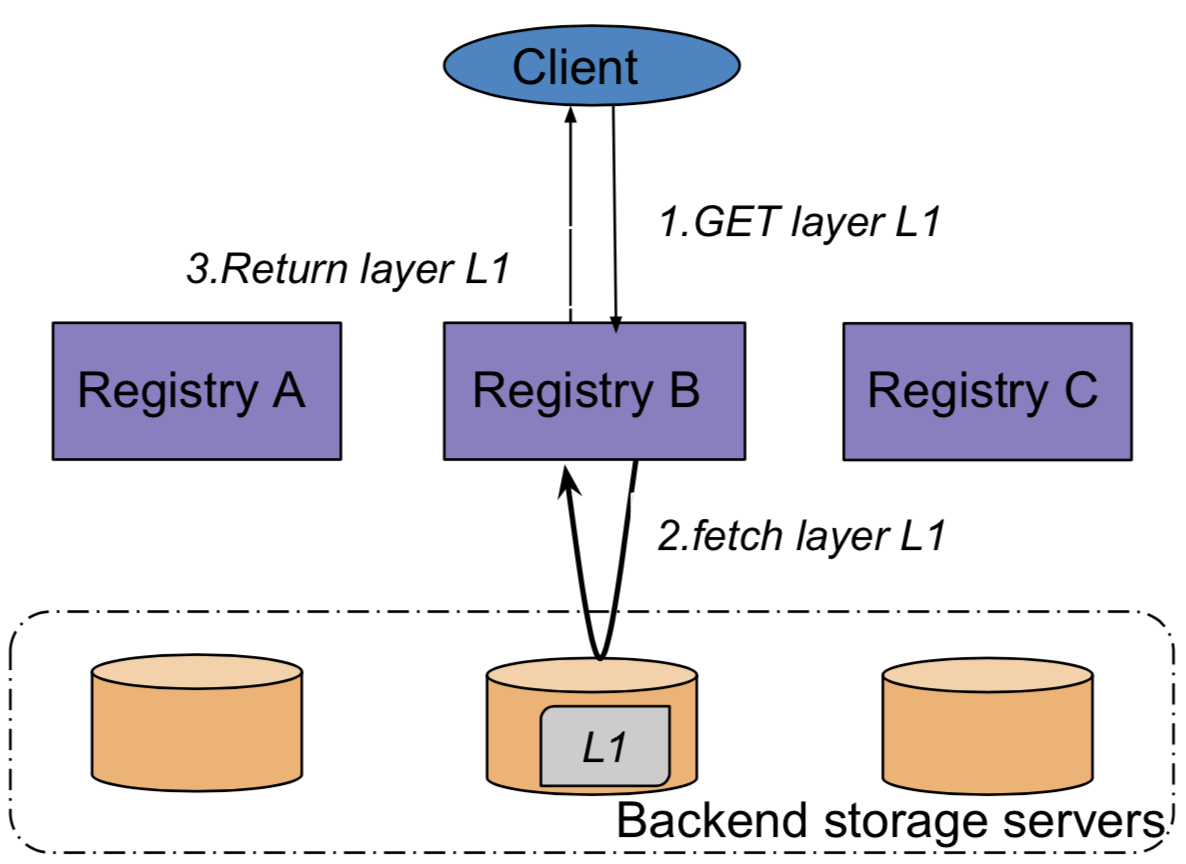
\includegraphics[width=1\textwidth]{graphs/nodedup.png}
			\caption{CDF of layer reference count.}
			\label{fig:ref_count}
		\end{minipage}
	\begin{minipage}{0.225\textwidth}
		\centering
		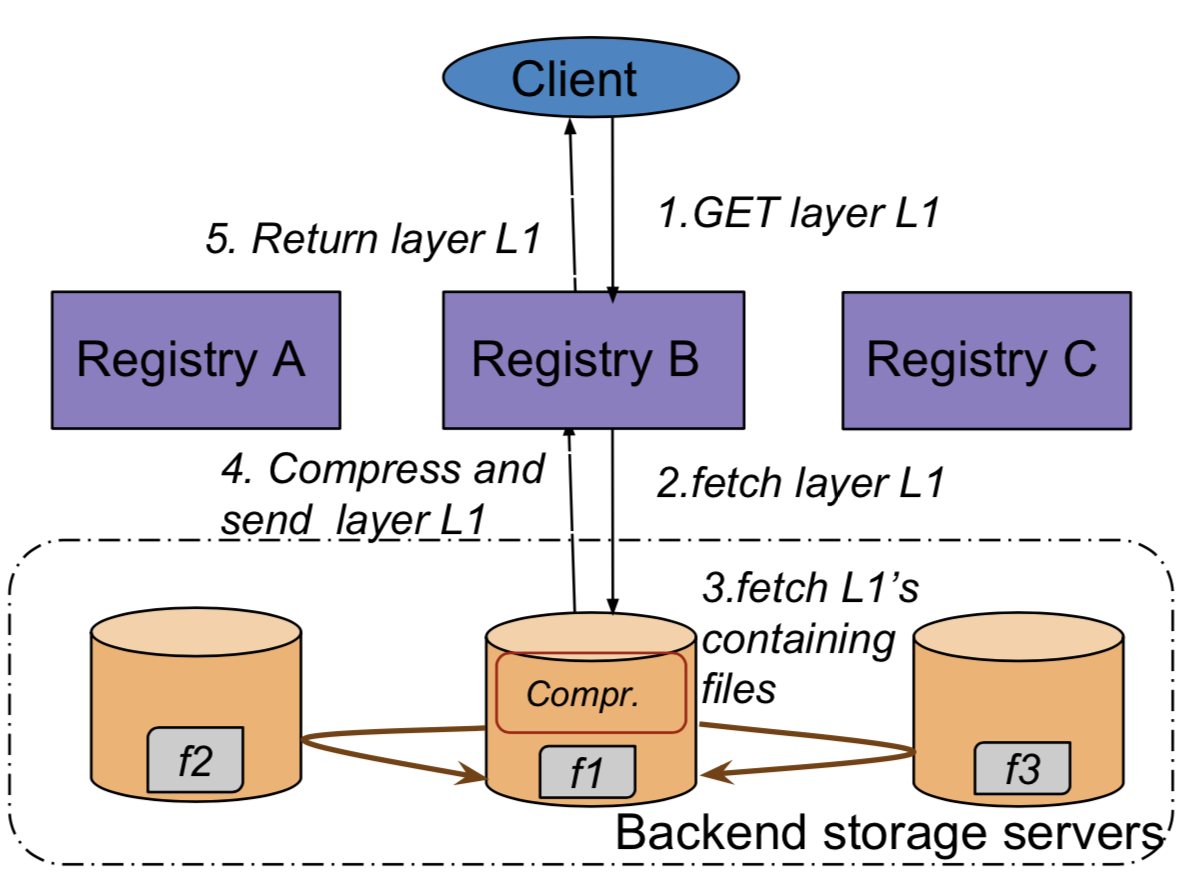
\includegraphics[width=1\textwidth]{graphs/dedup.png}
		\caption{CDF of compress. and uncompress. layer size.}
		\vspace{-3pt}
		\label{fig:nodedup-vs-dedup}
	\end{minipage}
\end{figure}

%\HA{need to mention Figure~\ref{fig:without-dedup} and Figure~\ref{fig:with-dedup}}

The organization of this paper as follows: 
We explain relevant Docker details along with observations and current deduplication practices in production registries in~\cref{sec:background}.
We present~\sysname~in~\cref{sec:\sysname} and ~\sysname's preliminary evaluation in~\cref{sec:Evaluation}. 
We discuss related work in~\cref{sec:related}.
Lastly, we conclude and discuss in~\cref{sec:conclusion} and~\cref{sec:discussion}.

%%%%%%%%%%%%%%%%%%%%%%%%%%%%%%%%%%%%%%%%%%%%%%%%%%%%%%%%%%%%%%%%%%%%%%%%%%%%%%
%                                                                            %
%                                OLD INTRO                                   %
%                                                                            %
%%%%%%%%%%%%%%%%%%%%%%%%%%%%%%%%%%%%%%%%%%%%%%%%%%%%%%%%%%%%%%%%%%%%%%%%%%%%%%

%\emph{Containers}~\cite{process-containers-linux} have recently gained
%significant traction due to their low overhead, fast deployment, and
%the rise of container management frameworks such as Docker~\cite{docker}.
%%
%Polls suggest that 87\% of enterprises are at various stages of adopting
%containers, and they are expected to constitute a \$2.7 billion
%market by 2020~\cite{container-grow-by2020}.
%
%Docker combines process containerization with efficient and effective packaging
%of complete runtime environments in so called {\em images}.
%%
%Images are composed of shareable and content addressable {\em layers}.
%%
%A layer is a set of files, which are compressed in a single archive.
%%
%Both images and layers are stored in a Docker \emph{registry} and accessed by
%clients as needed.
%%
%Since layers are uniquely identified by a collision-resistant hash of
%their content, no duplicate layers are stored in the registry.
%
%Registries are growing rapidly.
%%
%For example, Docker Hub~\cite{docker-hub}, the most widely used registry,
%stores more than 500,000 public image repositories comprising over 2 million
%layers and it keeps growing.
%%
%Over a period from June to September 2017, we observed a linear growth of the number
%of images in Docker Hub with an average creation rate of 1,241 repositories per day.
%%
%We expect this trend to continue as containers gain more popularity.
%%
%This massive image dataset presents challenges to the registry storage
%infrastructure and so far has remained largely unexplored.
%
%In this paper, we perform the first large-scale redundancy
%analysis of the images and layers stored in Docker Hub.
%%
%We downloaded 47\,TB (167\,TB uncompressed) worth of Docker Hub images,
%%
%which in total contain over 5 billion files.
%%
%Surprisingly, we found that only around 3\% of the files are unique
%while others are redundant copies. This suggests that current layer
%sharing cannot efficiently remove data duplicates.
%%
%We further analyzed the reasons for the high number of redundant files
%and found, for example, that different Docker images often
%contain the same source code from external public repositories
%(e.g., GitHub~\cite{github}).
%%
%%As there are no official images containing this source code, users manually add
%%it to their images, resulting in different layers which cannot be reused.
%
%Given our findings, we propose \sysname, a file-level content addressable storage
%model for the Docker registry.
%%
%\sysname\ unpacks layer tarballs into individual files and deduplicates them.
%%
%When a Docker client requests a layer, \sysname\ dynamically reconstructs the
%layer from its constituent files.
%%
%To assess the feasibility of our design, we conduct a simulation-based
%evaluation of \sysname. 
%%
%The simulation results show that \sysname\ improves the deduplication
%ratio from 1.8$\times$, provided by layer sharing, to 6.9$\times$.
%%provided by file-level deduplication.
%%
%While \sysname\ comes with some overhead 
%%when retrieving layers from the registry
%caused by the need to decompress and reconstruct layers, we found,
%for example, that for
%layers less than 10\,MB (around 60\% of all layers) the overhead of
%retrieving a layer is less than 1\,s.
%%
%For larger layers, we propose several optimizations to reduce overhead.
%\VT{Here we need to add 1-2 *most interesting* performance-related findings.}

%
%The simulation result show that 
%(1)~processing layers in
%parallel can largely improve throughput. For example, 80\% of file-level deduplication time is
%less than 9.09 s per layer and by processing 60 layers in parallel, our one-node
%prototype can process about 3 layers per second.
%
%\LR{That sounds like we actually ran the deduplication and not just simulated it?
%Did we perform more of an \emph{emulation}?}
%
%(2) Fast compression methods can mitigate pull overhead caused by re-compression
%because files are required to be re-compressed as a compressed layer archival file to serve
%the incoming pull requests.
%

%
%We make three major observations:
%
%\begin{compactitemize}
%
%\item Only 10\% of layers are referred to by more than one image, 
%meaning that layer-level content addressability is not enough to
%effectively reduce storage utilization in the registry.
%\DIM{Should we also provide the capacity \%?}
%
%\item A large amount of files are shared across layers and images,
%resulting in only 3\% of unique files.
%\DIM{Should we also provide the capacity \%?}
%
%\item Source code and scripts have a high deduplication ratio
%(\textbf{$31.25\times$} for source codes and \textbf{$50\times$} for scripts),
%which can result in executable and object file duplicates.
%
%\end{compactitemize}


%%%%%%%%%%%%%%%%%%%%%%%%%%%%%%%%%%%%%%%%%%%%%%%%%%%%%%%%%%%%%%%%%%%%%%%%%%%%%%
%                                                                            %
%                                OLD INTRO                                   %
%                                                                            %
%%%%%%%%%%%%%%%%%%%%%%%%%%%%%%%%%%%%%%%%%%%%%%%%%%%%%%%%%%%%%%%%%%%%%%%%%%%%%%

%Finally, we proposed and implemented Docker registry design that performs
%deduplication.
%%
%In our thorough redundant analysis and characterization of the xxxx images,
%with xxxx layers and xxxx files, we investigated the following four research
%questions (RQs):
%
%\begin{compactitemize}
%%
%\item How much redundant data stored in layers, images, and registry? Although
%layer-level address content addressable storage is adopted by Docker, we do not
%know whether  this coarse-grain layer-level content addressable storage (LLCAS)
%can efficiently reduce duplicates, and how much redundant data is stored in
%layer, image, and registry.
%%
%\item What are the redundant files and why there are so many redundant files?
%We aim to identify what are the redundant files that users mostly replicate.
%%
%Such information will provide Docker designer knowledge (user behavior) to
%better develop and optimize Docker container and Docker registry storage
%system.
%%
%\item What are the challenges faced by Docker registry and engine designer? By
%characterizing and analysis all the image metadata, we aim to identify the
%challenges' faced by registry designer and guide designers'optimization and
%users' development.
%%
%\item How to reduce the redundant files? We aim to propose a file-level content
%addressable model to reduce the redundant files by using file-level dedup while
%maintaining a good performance.
%%
%\end{compactitemize}
%
%The significance of this work are (1) our empirical evidence that large amount
%of redundant files exist in layers, images, and registry and layer-level
%content addressable storage is not efficient to remove redundant files;(2)
%findings about what are the redundant files and why there are so many redundant
%files exist;(3) first in-depth characterization on image dataset (union file
%systems)(4) a file-level content addressable model that can efficiently remove
%redundant copies while maintain a good performance.

%For years, virtual machines served as a cornerstone of computing resource
%virtualization both on premises and in the cloud~\cite{rosenblum2005virtual}.
%%
%Recently, however, \emph{container-based} virtualization started to gain
%significant traction~\cite{process-containers-linux}.
%%
%According to polls, over 87\% of enterprises are at various stages of adopting
%containers; analysts also predict that by 2020, containers will constitute a
%lucrative \$2.5 billion market~\cite{container-grow-by2020}.
%
%
%
%At its core, container is a set of processes which are isolated by the operating
%system kernel in terms of visibility and resources. This allows containers to share
%the same kernel without being aware of each other.
%%
%For example, Linux performs visibility isolation (for user identifiers, file systems,
%network, etc.) using namespaces~\cite{man-namespaces} and enforces resource
%utilization constraints with control groups~\cite{kernel-doc-cgroups}.
%%
%Compared to virtual machines, containers use less memory and storage, are much
%faster to start, and typically cause less execution
%overhead~\cite{felter2015updated, Disco, HypervisorsvsLightweight}.
%
%The rapid increase in use of container technology was largely made possible by
%container management frameworks, with Docker being one of the most popular
%solutions~\cite{docker}.
%%
%Docker combines process containerization with efficient and effective runtime
%environment packaging.
%%
%Software is packaged in container \emph{images}, each consisting of several
%read-only \emph{layers} and a manifest which describes container metadata, \eg
%what layers make up an image and which command to run at container startup.
%%
%Read-only layers can be shared between different images and encapsulate
%file-system trees for dockerized processes.
%
%%Docker is another technology whose popularity grew rapidly in the recent
%%years~\cite{docker}.
%%
%%When Docker starts a container, it combines read-only layers (and an additional
%%writable layer to store changes) into a single namespace and starts the process
%%declared in the manifest in the new namespace~\cite{docker-driver-eval}.
%
%
%
%Docker images are stored in a centralized \emph{registry} and are pushed to and
%pulled from the registry by clients as needed.
%%
%Docker Hub~\cite{docker-hub} is the most widely used Docker registry
%installation which, according to our estimates, stores more than 400,000
%\emph{public} image repositories comprising a total of 2 million layers.
%%
%This amount is steadily increasing and we observed a linear growth of the
%number of images over a period from June to September 2017.
%
%
%
%While this massive dataset presents challenges to the registry storage
%infrastructure, it also provides opportunities to better understand how
%containers are used in practice.
%%
%Currently, there is little known about the contents, use cases, and workloads
%of production containers.
%%
%In part, this is due to the privacy concerns that organizations and individuals
%have when sharing details of their computing environments.
%%
%However, this knowledge is imperative to design and evaluate novel approaches
%to improve the performance and reliability of containers.
%
%
%
%
%In particular, storage for containers has remained a largely unexplored
%area~\cite{login-container-storage-options}.
%%
%We believe one of the prime reasons is the limited understanding of what data
%is stored inside containers.
%%
%This knowledge can not only help to directly improve the registry and container
%storage infrastructure but also allows to infer container use cases and derive
%representative workloads from that.
%%
%While existing work as focused on various aspects of
%containerization~\cite{slacker, dockervulnerabile, dockerfinder, analysisdockergithub, dockerssd}, analyzing the
%contents of images and layers has not received much attention.
%
%
%
%
%%Though much research was focused on various aspects of
%%containerization~\cite{prev-work-1, prev-work-2, prev-work-3}, storage for containers
%%remains an unexplored territory~\cite{login-container-storage-options}.
%%
%%To start designing a novel storage solution for containers,
%%or to optimize and fairly evaluate existing ones,
%%it is imperative to understand containers' real-world
%%use cases and workloads in sufficient details.
%%
%%Unfortunately, little is known about how containers are used in the real world.
%%
%%In part, this is due to the privacy concerns that organizations and individuals
%%have when sharing details of their computing environments.
%
%
%%Docker images are stored at the centralized \emph{registry} and are pushed to
%%and pulled from the registry by clients as needed. 
%%
%%The most known Docker registry installation is Docker Hub which according to
%%our estimates stores at least 400,000 \emph{public} images that consist of at
%%least 2,000,000 layers.
%
%
%
%
%In this paper we perform the first, comprehensive, large-scale characterization of
%Docker registry contents.
%%
%We downloaded over 50TB of Docker images from Docker Hub and analyzed
%traditional storage properties---\eg, file sizes and types, data compression
%ratios, directory depths---as well as Docker-specific properties---e.g., the number
%of layers per image and the amount of layer sharing.
%%
%%Our insight in this study is that this massive dataset can be used to understand what
%%applications run in containers, how much data they store, and the properties of
%%the data.
%%
%We found, for example:
%\begin{compactenumerate}
%	\item 90\% of the repositories only have a very small pull count (less than 333), which suggests that Docker hub is a good fit for caching few popular repositories or images.
%	\item majority of the images and layers in Docker hub have a smaller size. 90\% of images can be compressed with less than 500 MB and 70\% of images are less than 500 MB even without compression. 90\% of layer can be compressed with less than 63 MB and 77\% of layers are less than 63 MB even without compression.
%	\item Docker images has a great potential for compression to save space.
%	\item 90\% of images have less than 18 layers. Half of images have less than 8 layers. 
%	\item 10\% of layers are referenced more than one image.
%	\item Around 90\% of layers' directory depth is less than 30. 50\% of layers' directory depth is less than ~3.
%	\item Around 30\% of files are ASCII text files. 
%	About 11\% files are gzip compressed files 
%	Interestingly, about 1\% of files are empty. 
%\end{compactenumerate}
%%
%\vcomment{Here we need to stick an example or two of interesting findings. \nancomment{addressed}}
%
%%From our findings, we infer a set of propositions to describe how Docker is
%%used in the real world:
%%\lrcomment{Can we summarize our findings in a few propositions to put here?}.
%%
%%We believe our findings will improve the understanding of containers' data and lay
%%a solid ground for future storage optimizations at clients and registries in
%%Docker and beyond.
%
%After introducing the Docker background~(\S\ref{sec:background}),
%this paper makes the following contributions:
%\begin{compactenumerate}
%  \item We describe a comprehensive methodology to retrieve the complete set of
%  	images stored in Docker Hub~(\S\ref{sec:methodology});
%  \item We perform the first in-depth analysis of container images stored in
%    Docker Hub~(\S\ref{sec:char}).
%%  \item based on our analysis, we formulate propositions on how Docker is currently
%%    used to help guide optimizations and benchmark
%%    workloads~(\S\ref{sec:propositions}).
%\end{compactenumerate}
%
%After discussing related work~(\S\ref{sec:related}),
%the paper concludes~(\S\ref{sec:conclusion}).
%
%%The rest of the paper is organized as follows. We explain
%%relevant Docker details in Section~\ref{sec:background} and our methodology in
%%Section~\ref{sec:methodology}. We present dataset characterization in
%%Section~\ref{sec:results}, describe related work in Section~\ref{sec:related},
%%and conclude in Section~\ref{sec:conclusion}.


% \section{Background}
\label{sec:background}

Docker~\cite{docker} is a popular virtualization technology
that extends traditional OS containers with higher level
functionalities.
%
It allows to efficiently package an application and its runtime dependencies
in a container image to simplify and automate application deployment~\cite{slacker}.
%
%It automates the deployment of software and allows to efficiently package an
%application with its runtime dependencies in a container image~\cite{slacker}.
%


\begin{figure}
	\centering
	% Requires \usepackage{graphicx}
	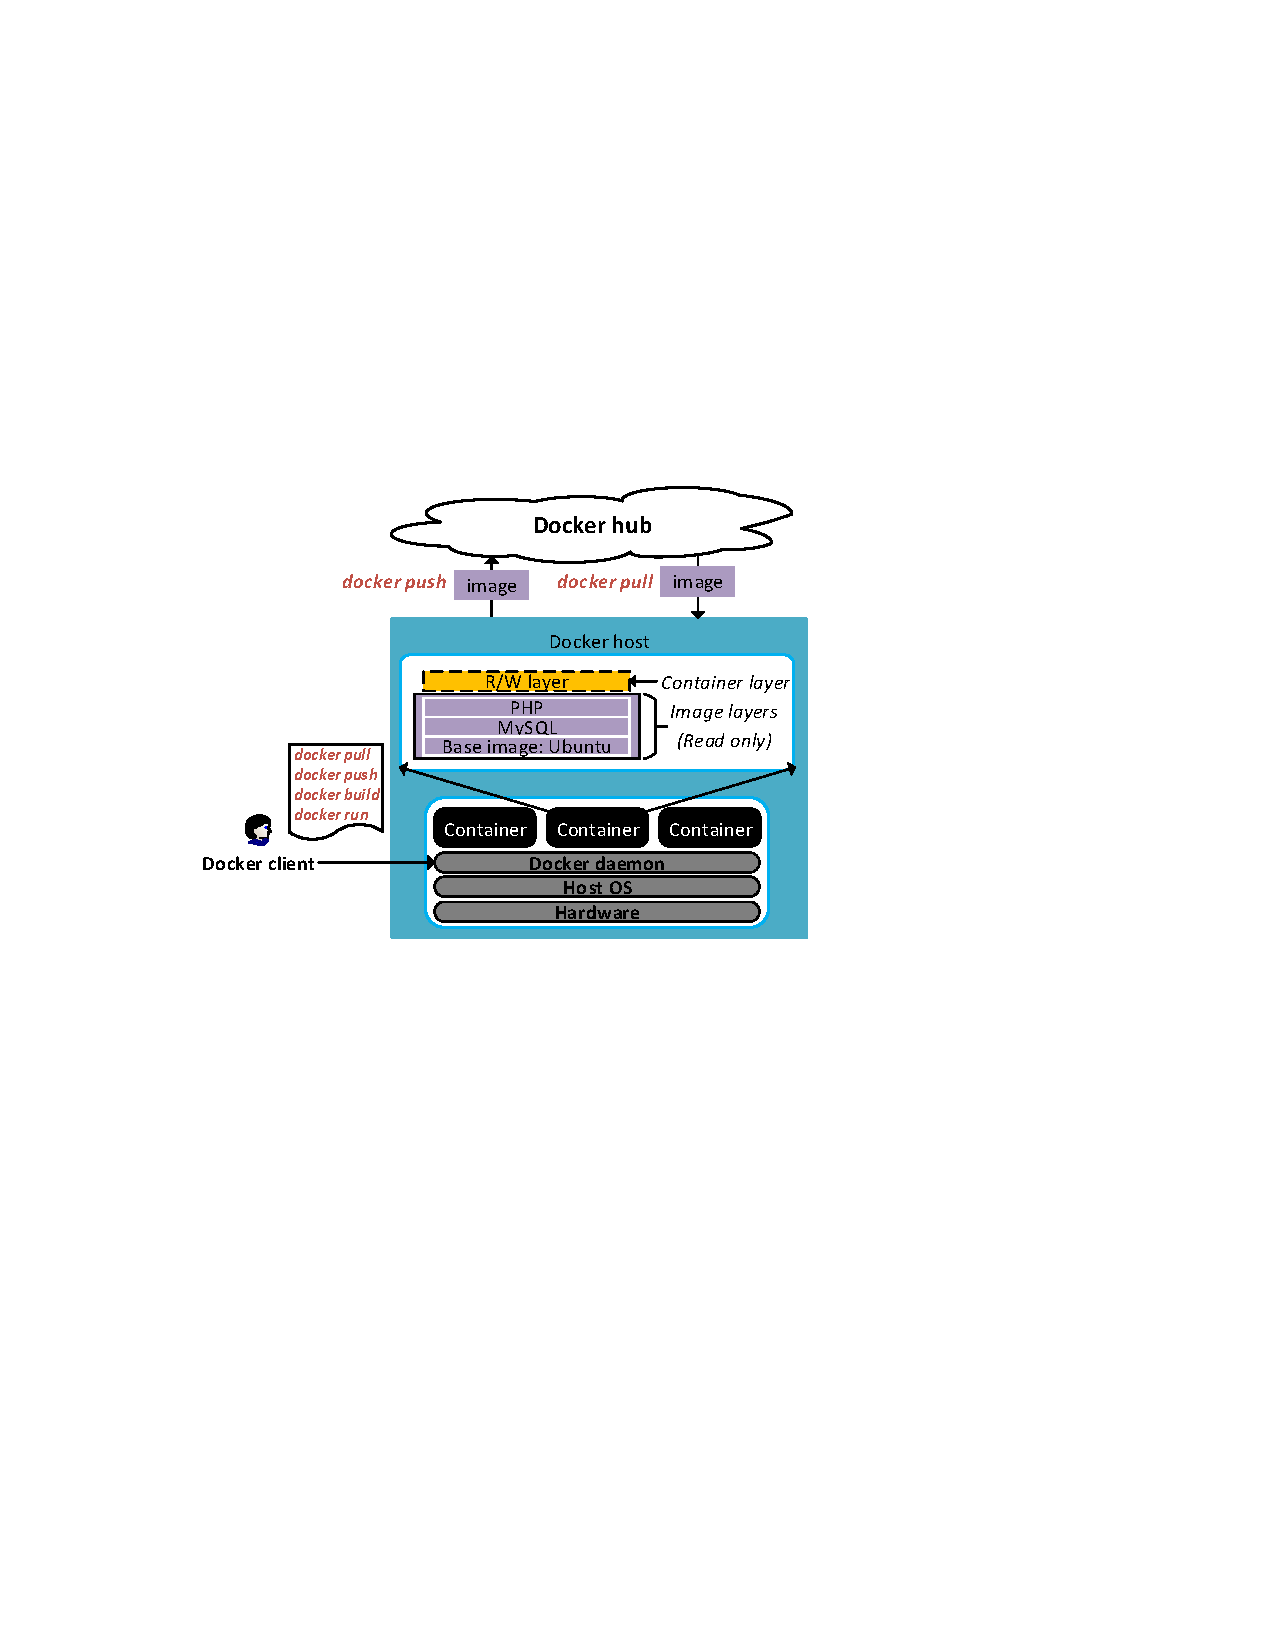
\includegraphics[width=0.5\textwidth]{graphs/fig-docker-architecture}
	\caption{Docker ecosystem
%	\lrcomment{We need to update the figure to capture
%	all the main interactions between the components and remove some unneeded
%	detail, \eg official and unofficial repositories\nancomment{addressed}}
	}
	\label{fig-docker-architecture}
\end{figure}
%
As shown in Figure~\ref{fig-docker-architecture}, a typical
Docker setup consists of three main components: 1)~\emph{client},
2)~\emph{host}, and 3)~\emph{registry}.
%
Users interact with Docker using the Docker client which, in turn,
sends commands to the Docker host.
%
Both client and host can run on the same machine.
%
Docker host runs a daemon process that implements the core logic of Docker and
is responsible for \emph{running} containers from locally available
images.
%
If a user tries to launch a container from an image that is not available
locally, the daemon \emph{pull}s the required image from the Docker registry.
%
Additionally, the daemon supports \emph{building} new images and \emph{pushing}
them to the registry.

\paragraph{Images and layers}
%
At the center of Docker is the concept of container images for packaging,
distributing, and running applications.
%
A Docker image consists of an ordered series of \emph{layers}.
%
Each Docker layer contains a subset of the files in the image and often represents a
specific component/dependency of the image, \eg a shared library.
%
Layers can be shared between two or more images if
the images depend on the same component.

Image layers are read-only.
%
When users start a container, Docker creates a new
\emph{writable layer} on top of the underlying read-only layers
(Figure~\ref{fig-docker-architecture}).
%
Any changes made to files in the image will be reflected inside the writable
layer via a copy-on-write mechanism~\cite{docker-driver-eval}.
%
This leaves layers unmodified throughout the lifetime of a container and
enables layer sharing between multiple containers spawned from the same or
different images.
%
%Docker supports multiple \emph{storage drivers} such as Aufs or Btrfs, which
%efficiently combine read-only and writable layers in a single
%namespace~\cite{docker-driver-eval}.
%
%The writable layers are deleted when the container is deleted.

%Image is represented by a \emph{manifest} which describes the various
%constituents of a Docker image, such as the target hardware platform and
%environment settings.
%%
%Moreover, the manifest contains a list of layer digests for all layers required
%by the image.


\paragraph{Registry}
%
The Docker registry is a platform for storing and sharing container images.
%
It stores images in \emph{repositories}, each containing different versions of
the same image. 
%
For each image Docker registry stores a \emph{manifest} that describes,
among other things, which layers constitute the image.
%
%The manifest is a JSON file, which contains the runtime configuration for a
%container image (\eg target platform and environment variables) and the list
%of layers which make up the image.
%
Layers are identified via a digest that is computed as a hash (SHA-256)
over the layers' uncompressed content and stored as compressed archival files.
%
%Image layers are stored as compressed archival files and image
%manifests as JSON files.
%
%\VT{What is image manifest? Need to introduce}
%
%
%Docker Hub is one of the most popular public registries, supporting both
%public and private repositories, via which users can upload, search, and
%download images~\cite{docker-hub}.
%
%In Docker Hub, the user repositories are namespaced by user name, i.e.,
%``$\langle username\rangle/\langle repository name \rangle$", while the
%official repositories, which are directly provided by Docker Inc. and partners
%are called ``$\langle repository name \rangle$".

%Modern Docker registry identifies and addresses a layer with a digest that is
%computed based on the uncompressed layer's content (e.g., SHA-256).
%
Identifying layers by their content allows the registry to store only one instance
of a layer even if it is referenced by multiple images.
%
\LR{Is that actually done across the entire registry or only within a single
user/repository? \NZ{entire registry}}
%multiple users accidentally built identical layers.
%
However, if at least one file differs in two otherwise identical layers,
the two layers are treated as different and stored separately.

\section{Background, observations, and motivation}
\label{sec:dataset-analysis}

%\subsection{Layer size distribution}
%
%\subsection{File size distribution}
%
%\subsection{Redundant file distribution}

%\section{Deduplication performance analysis} % just find the problem and benefit
\label{sec:background}

%\paragraph{Deduplication for improving storage capacity.}

On-cloud global deduplication software is widely adopted by cloud enterprises for reducing cloud storage consumption and overall storage cost. 
For example, StorReduce~\cite{storReduce}, the deduplication software used by
Google cloud and AWS, 
performs in-line transparent data deduplication. 
%StorReduce resides between the client's application and the hosting cloud storage.
%A number of deduplication methods focus on client-side data deduplication to ensure that only unique files are uploaded, 
%to save network bandwidth, by having the client send a duplicate check request~\cite{xxx}~\cite{xxx}. 
%For example, xxxx\NZ{Hadeel, can you add one example and few relatedwork citation?}. 
Intuitively, such deduplication techniques can be leveraged to eliminate redundant data from the Docker image storage system.  
Except, the Docker image dataset is not amenable to deduplication 
as the images are \emph{compressed archival files}.
%Intuitively, registries can be deployed as a proxy cache to host frequently requested layers to speedup image pulls and improve performance 
%while the backend cloud storage can leverage deduplication to save storage space.
%However, there are several unique problems concerning the integration of caching and deduplication to the unique Docker registries workload: \textbf{compressed layers}. 
%We investigate the potential for data reduction in the Docker registry by estimating the efficacy of layer sharing and file-level deduplication.
%We noticed that the number of public repositories is constantly increasing with a growth that amounts 
%to around 1 million repositories annually. 
%This corresponds to~130\,TB of annual growth in storage needs 
%\HA{but it is actually less because of shared layers, right?}, 
%costing around~\$15,000 a month if Google Cloud Storage is used~\cite{GoogleCloudStoragePricing}.
%This growth implies significant benefits to data deduplication. 


As discussed in~\cref{sec:intro}, only $3$\% of the files in a sample Docker hub image collection were found to be unique, mainly becuase 
 compressed files have a very low deduplication ratio~\cite{meister2012study}.
Thus, 
we can realize significant space savings if we can remove the 
duplicate files. This entails decompressing files before performing deduplication, and collecting components of layers from multiple servers.
%
To quantify the performance overhead of such an approach involving decompressing, deduplication, and then re-compressing,
we setup five registry instances. Each instance has a local file system as their backend storage system. We
implemented file-level deduplication with decompression and compression operations.
We replayed the IBM registry workload \texttt{dal}~\cite{dockerworkload} 
%by sending requests randomly 
randomly to our five registries and measured the latency. 
%
Figure~\ref{fig:avg_latency_dedup_nodedup} shows the average latency observed 
across five registries.
%\arb{average across what??}\NZ{addressed}.
Note that since 
%the IBM registry workload 
\texttt{dal} does not contain real layers,
we extract the layer digest from each request and match it with a layer randomly selected from our Docker Hub dataset to emulate realistic requests.

Without deduplication,
the average latency for requesting a layer is about $2$~s for layers with sizes $\textless50$~MB.
The latency increases to $12$~s when the above deduplication is implemented in the backend storage system.
Furthermore, Docker registry performance drops down dramatically for larger layers.
We observe that the average latency for requesting layers $\textgreater50$~MB and $\textless1$~GB
is about $128$~s. The latency worsens with dedupliation to on average of about $800$~s.
%\NZ{todo:graph: less than, }
%\HA{running five registries, replaying dal trace using trace replayer-cite, and since the replayer doesn't use real layers we randomly match the request to our dataset downloaded from docker hub. describe how we got these numbers. for dedup, we simply implemented a decompress/compress + file-level deduplication on backend storage systems, we use a CHT based distributed storage system. Figure~\ref{fig:avg_latency_dedup_nodedup}}
\begin{figure}[t]
	\centering
	%\scriptsize
	\begin{minipage}{0.225\textwidth}
		\centering
		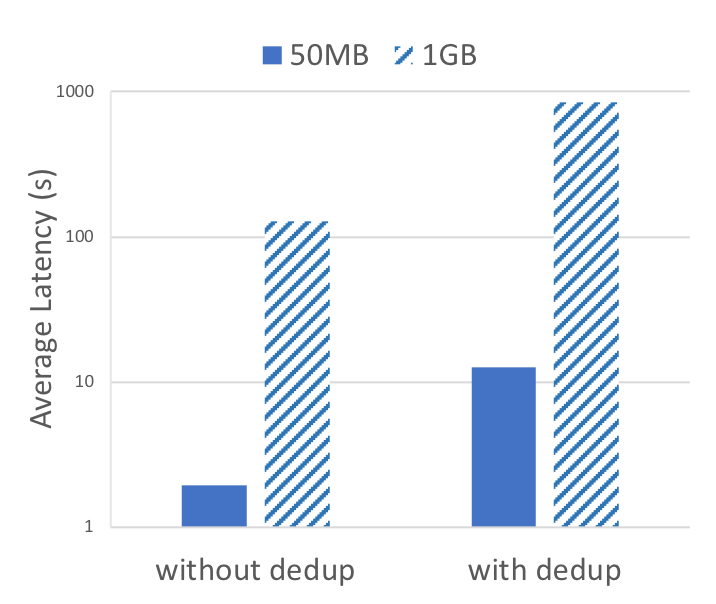
\includegraphics[width=1\textwidth]{graphs/avglatency_dedup_nodedup.png}
		\caption{Average latency.}
		\label{fig:avg_latency_dedup_nodedup}
	\end{minipage}
	\begin{minipage}{0.225\textwidth}
		\centering
		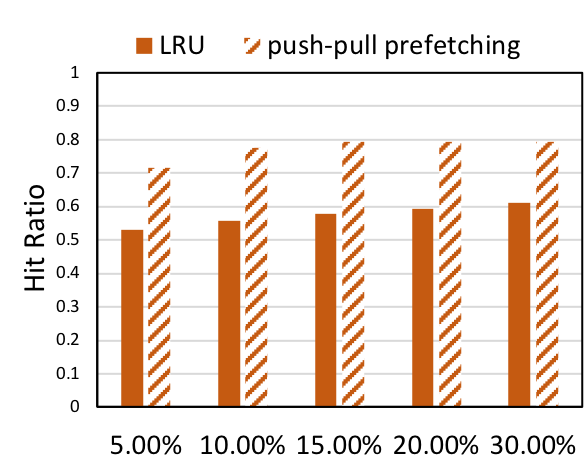
\includegraphics[width=1\textwidth]{graphs/lru_prefetch_hits.png}
		\caption{Hit ratio.}
		\vspace{-3pt}
		\label{fig:lru_prefetching_hits}
	\end{minipage}
\end{figure}
% for LRU and push-pull prefetching under different cache sizes (\% of total accessed layers).



%\begin{figure*}[t]
\centering
			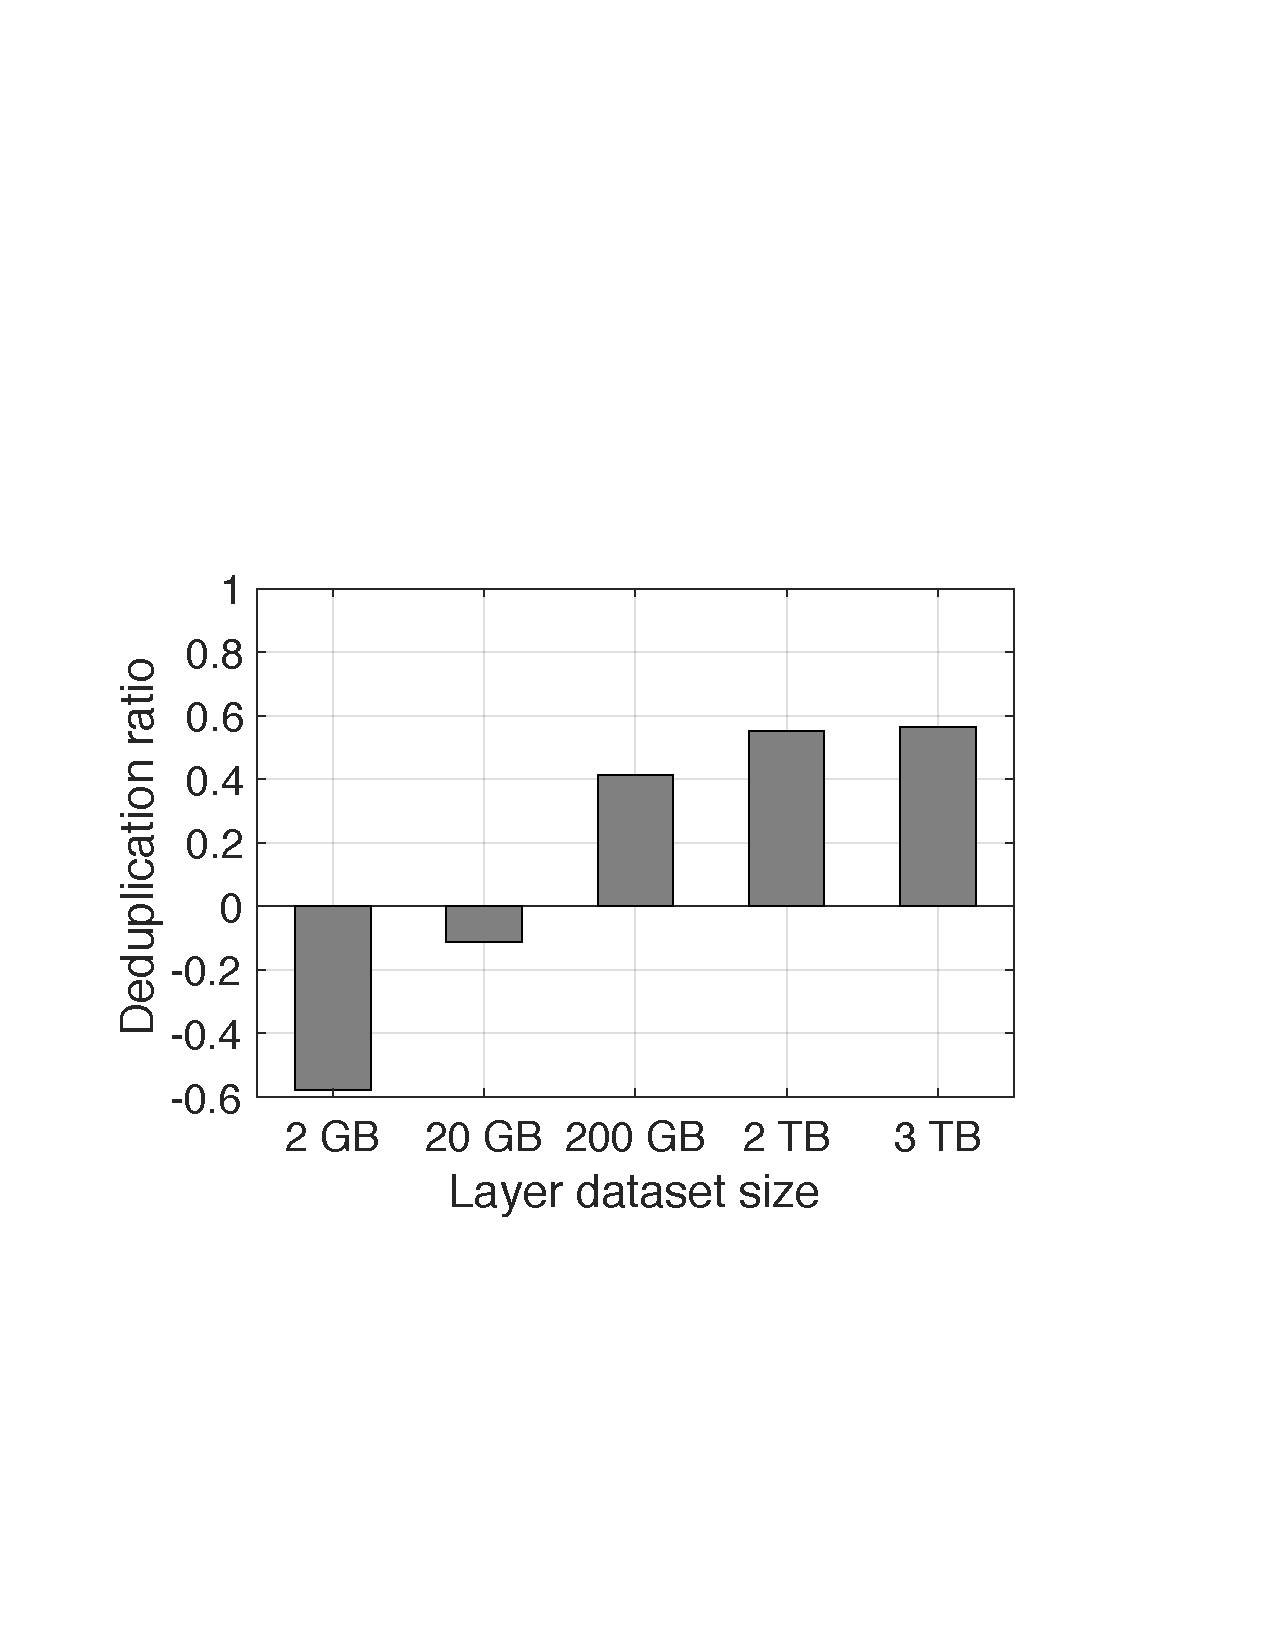
\includegraphics[width=0.2\textwidth]{graphs/dedup_vs_compression.pdf}
			\caption{Efficiency of deduplication over compression}
		%	\vspace{-3pt}
			\label{fig:cacheefficiency}

\end{figure*}

%\begin{figure}[t]
%	\centering
%	\begin{minipage}{0.26\textwidth}
%		\centering
%		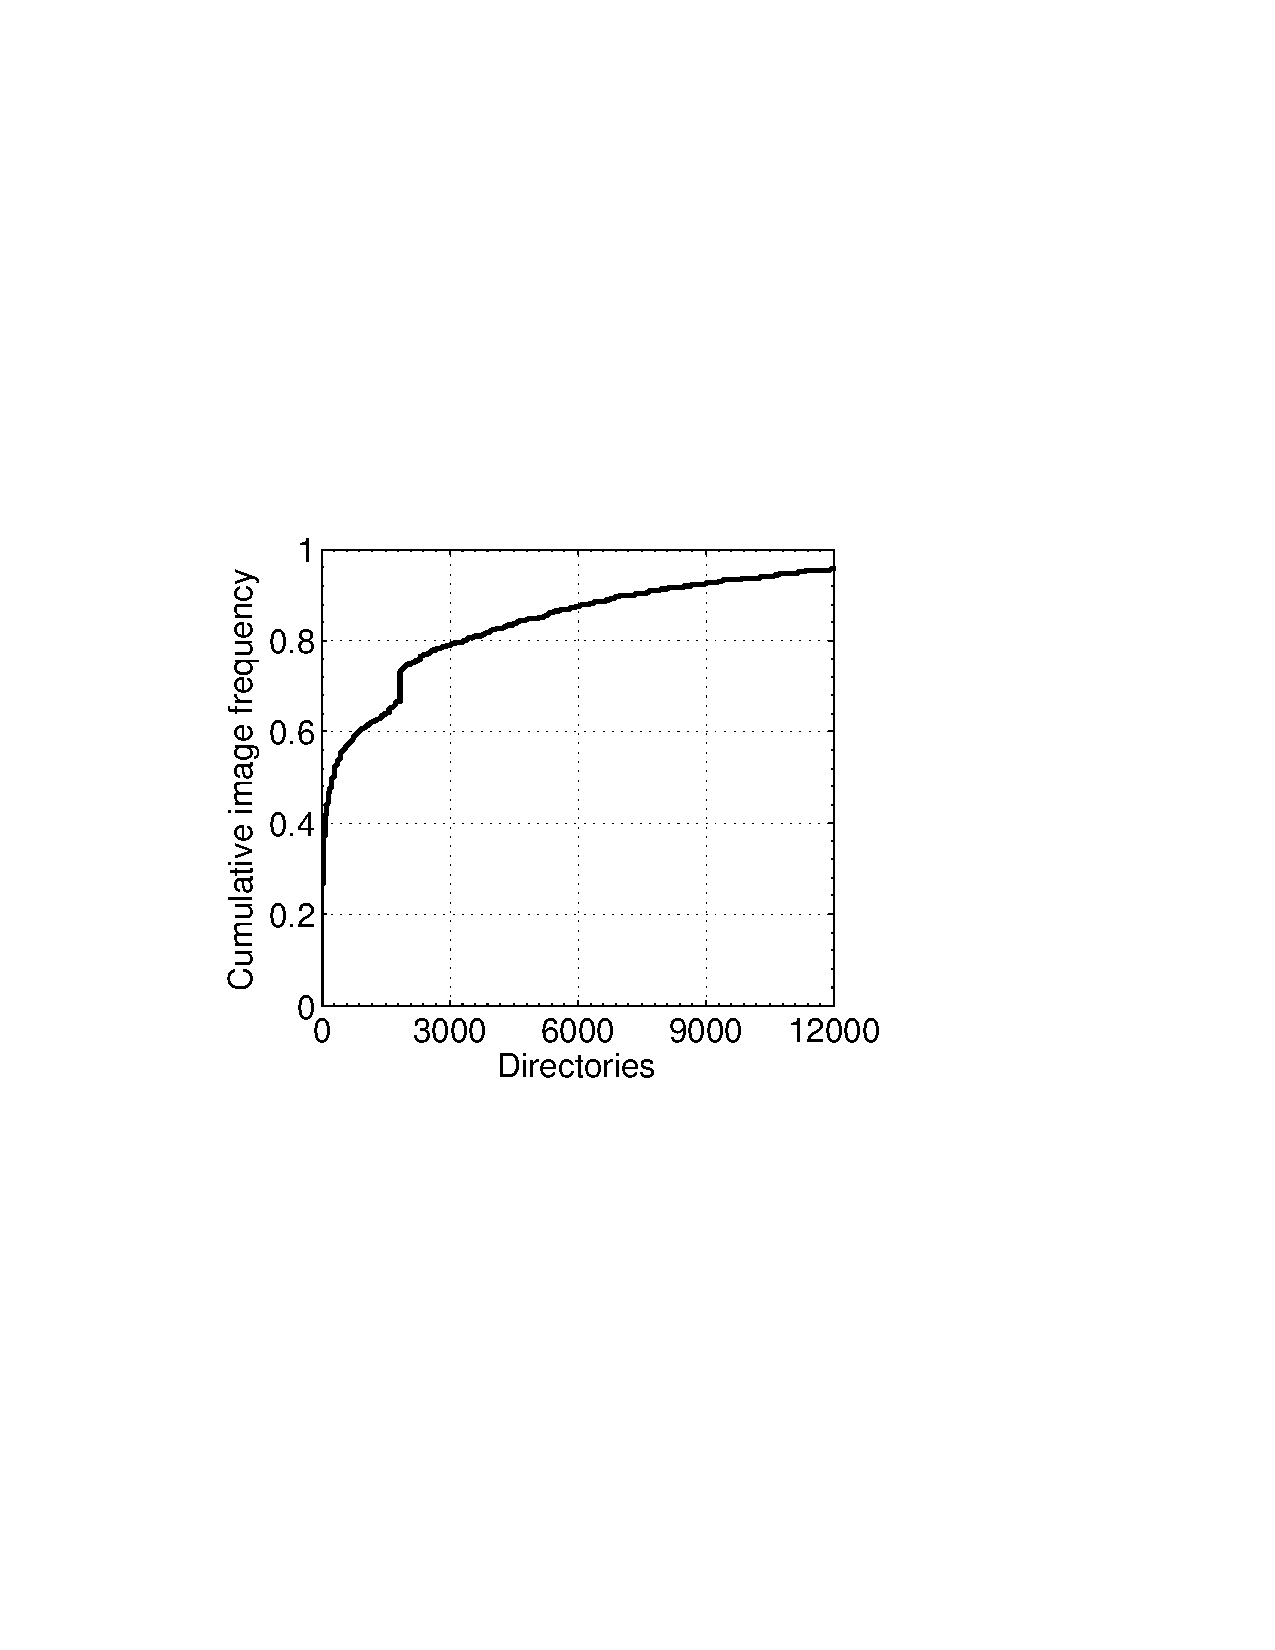
\includegraphics[width=1\textwidth]{graphs/dir.pdf}
%		\caption{CDF of images by\newline directories}
%		\label{fig-dir}
%	\end{minipage}%
%	\begin{minipage}{0.24\textwidth}
%		\centering
%		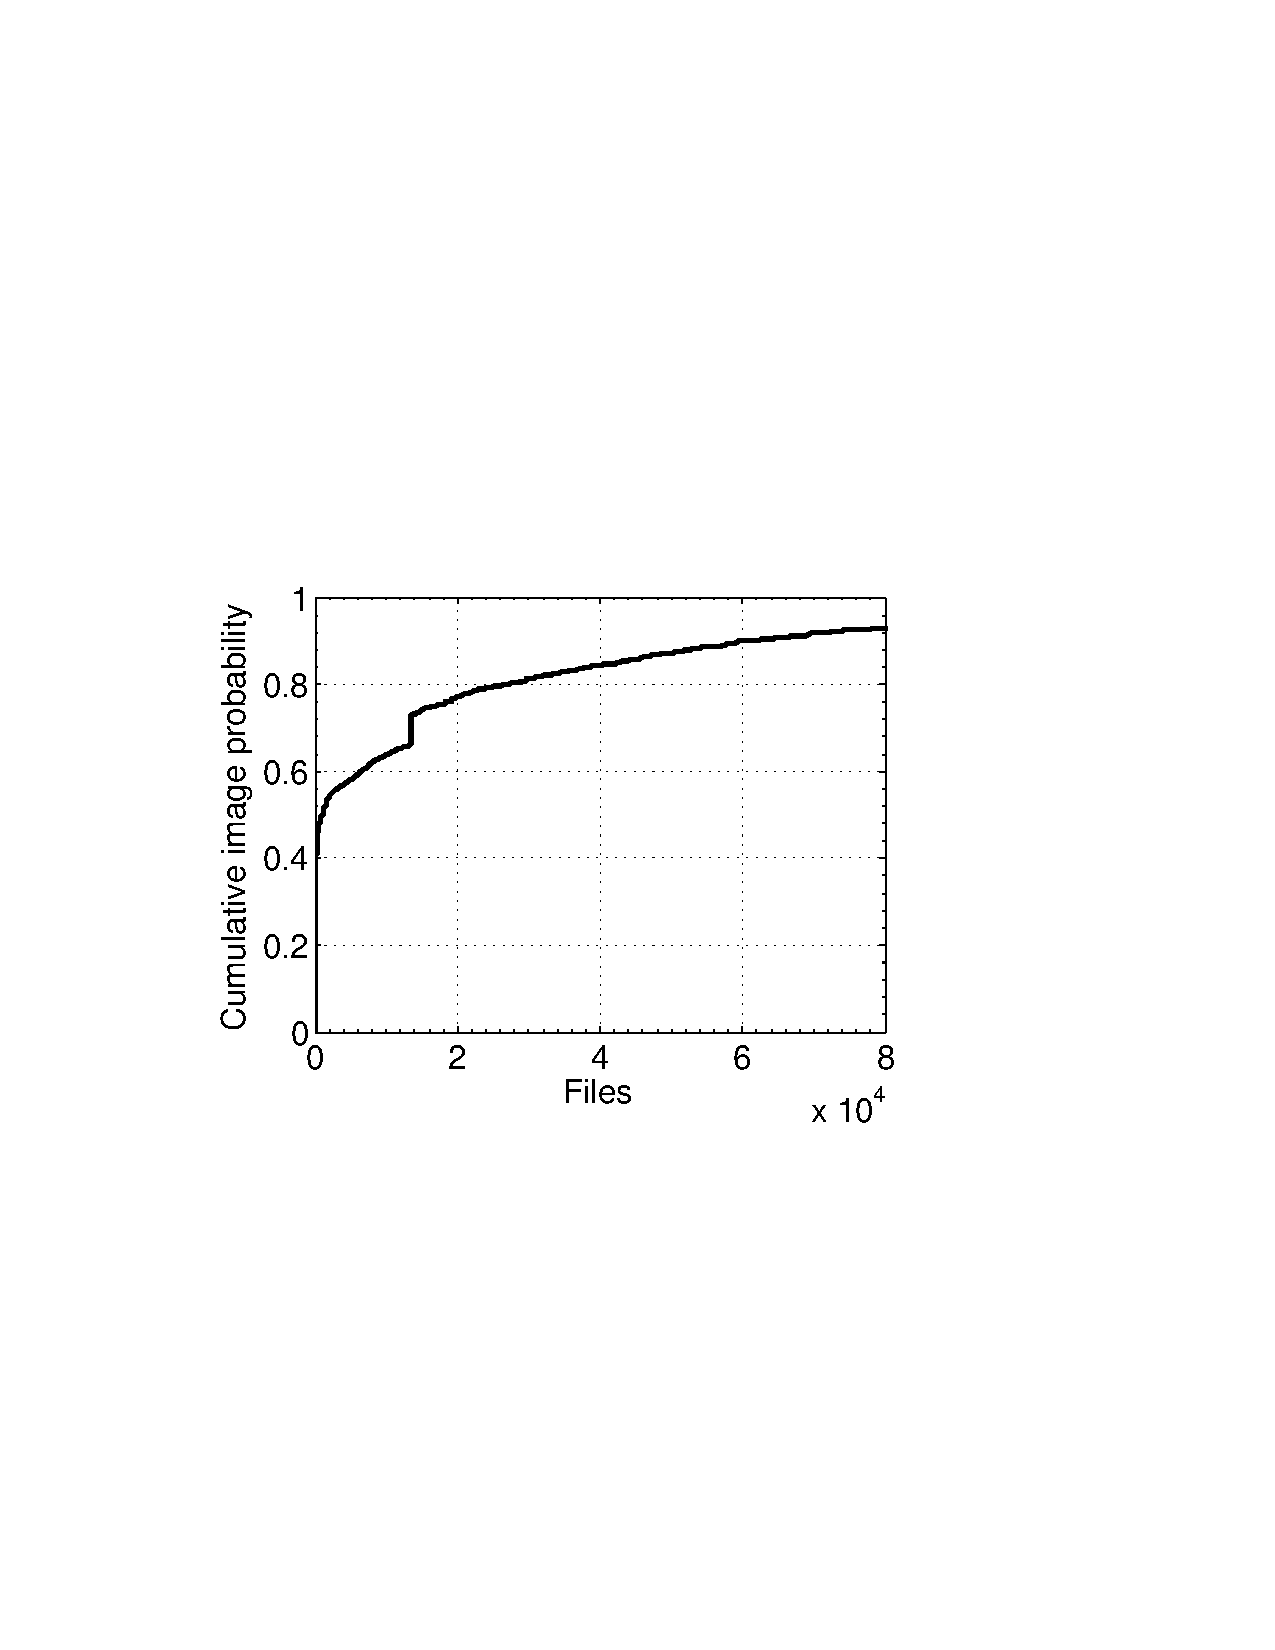
\includegraphics[width=1\textwidth]{graphs/file.pdf}
%		\caption{CDF of images by files}
%		\label{fig-file}
%	\end{minipage}
%\end{figure}

%\begin{figure}[htbp] 
%	\begin{minipage}{0.5\linewidth} 
%		\centering 
%		\includegraphics{circle} 
%		\caption{A Circle} 
%		\label{fig:circle} 
%	\end{minipage}% 
%	\begin{minipage}{0.5\linewidth} 
%		\centering 
%		\includegraphics{rectangle} 
%		\caption{A Rectangle} 
%		\label{fig:rectangle} 
%	\end{minipage} 
%\end{figure}

\subsection{Inter-layer deduplication}

\paragraph{Duplicated files shared among layers}
Although Docker uses COW file system to minimize redundant data inside each image and
 supports the sharing of layers among different images to remove redundant data in Docker registry backend storage system,
 a large amount of duplicated files are observed among layers within different images.  
According to the deduplication analysis on Docker Hub dataset~\cite{dedupanalysis},
only 3.2\% of files are unique, resulting in deduplication ratio of 2x in terms of capacity. 
These large amount of duplicated files %shared among different layers associated with different images
are mainly executables, object codes, libraries, and source codes probably
imported by different image developers using the same package installers or version control systems such as
\texttt{apt},  \texttt{pip} or \texttt{git} to install or get similar dependencies or source codes.
The file-level duplication among different layers cannot be \emph{deduplicated} 
by using layer-level content addressable storage system adopted by current registry.

\paragraph{Layer deduplication}
As containerization frameworks like Docker and Kubernetes keep gaining in popularity,
more applications are encapsulated into images, pushed into registry, and stored on Cloud.
By using \emph{R}-way replication, the amount of layers grows exponentially and will explode in future.
This is not just a requirement of more disks.
It goes beyond just hardware upgrade or even datacenter expansion,
and into large volumes of data management challenges, such as missive and slow data migration during scale-out or scale-up.
 
File-level deduplication can be implemented on registry by first decompressing the compressed layer tarballs and 
removing the duplicated files across different layers.
In this case, 
layer dataset stored on registry can be largely reduced for good data management.
However,  
\texttt{pulling}
a layer from registry requires restoring a layer,
which involves file fetching, layer archiving, and layer compression.
These extra operations incurs a considerable overhead especially for  
\texttt{pulling} layer performance which is crucial for container startups. 
Is it possible to deduplicate layers while maintaining a good layer \texttt{pulling} performance?
We analyze registry workloads and 
optimize the performance by exploring workload patterns and user access patterns.   
%Consider that deduplication incurs a performance overhead and the current Docker registry already stores layers in compressed format to save space and network transfer overhead. We first analyze the space efficiency of a registry that performs decompression and file-level deduplication and compare it to a registry that naively stores compressed layers.

%In Figure~\ref{fig:cacheefficiency}, the x-axis values correspond to the sizes of $5$ samples of registry data of varying sizes with traditional layer compression. For a traditional registry, the compressed layer tarballs will be kept as is.
%While a registry with file-level deduplication will store \emph{deduplicated} layers (i.e., unique files). 
%The y-axis shows how much space a registry with file-level deduplication can save over compressed layer tarballs.
%For the first two samples of the dataset, with size less than $20$~GB, 
%there is no benefit to \emph{deduplicate} layers because the deduplication ratio is very low.
%However, when the dataset size is $200$~GB and over, we can save over $40\%$ more space increasing almost linearly with the size of the layer dataset.
%This verifies the benefit of deduplicating layers as the registry size increases.
%Before describing Sift, we must understand the storage pressure and trends in the access patterns of the Docker registries at the layer and repository level.

\subsection{Predictable User Access}
%\begin{figure*}[t]
%		\begin{minipage}{0.32\linewidth}
%			\centering
%			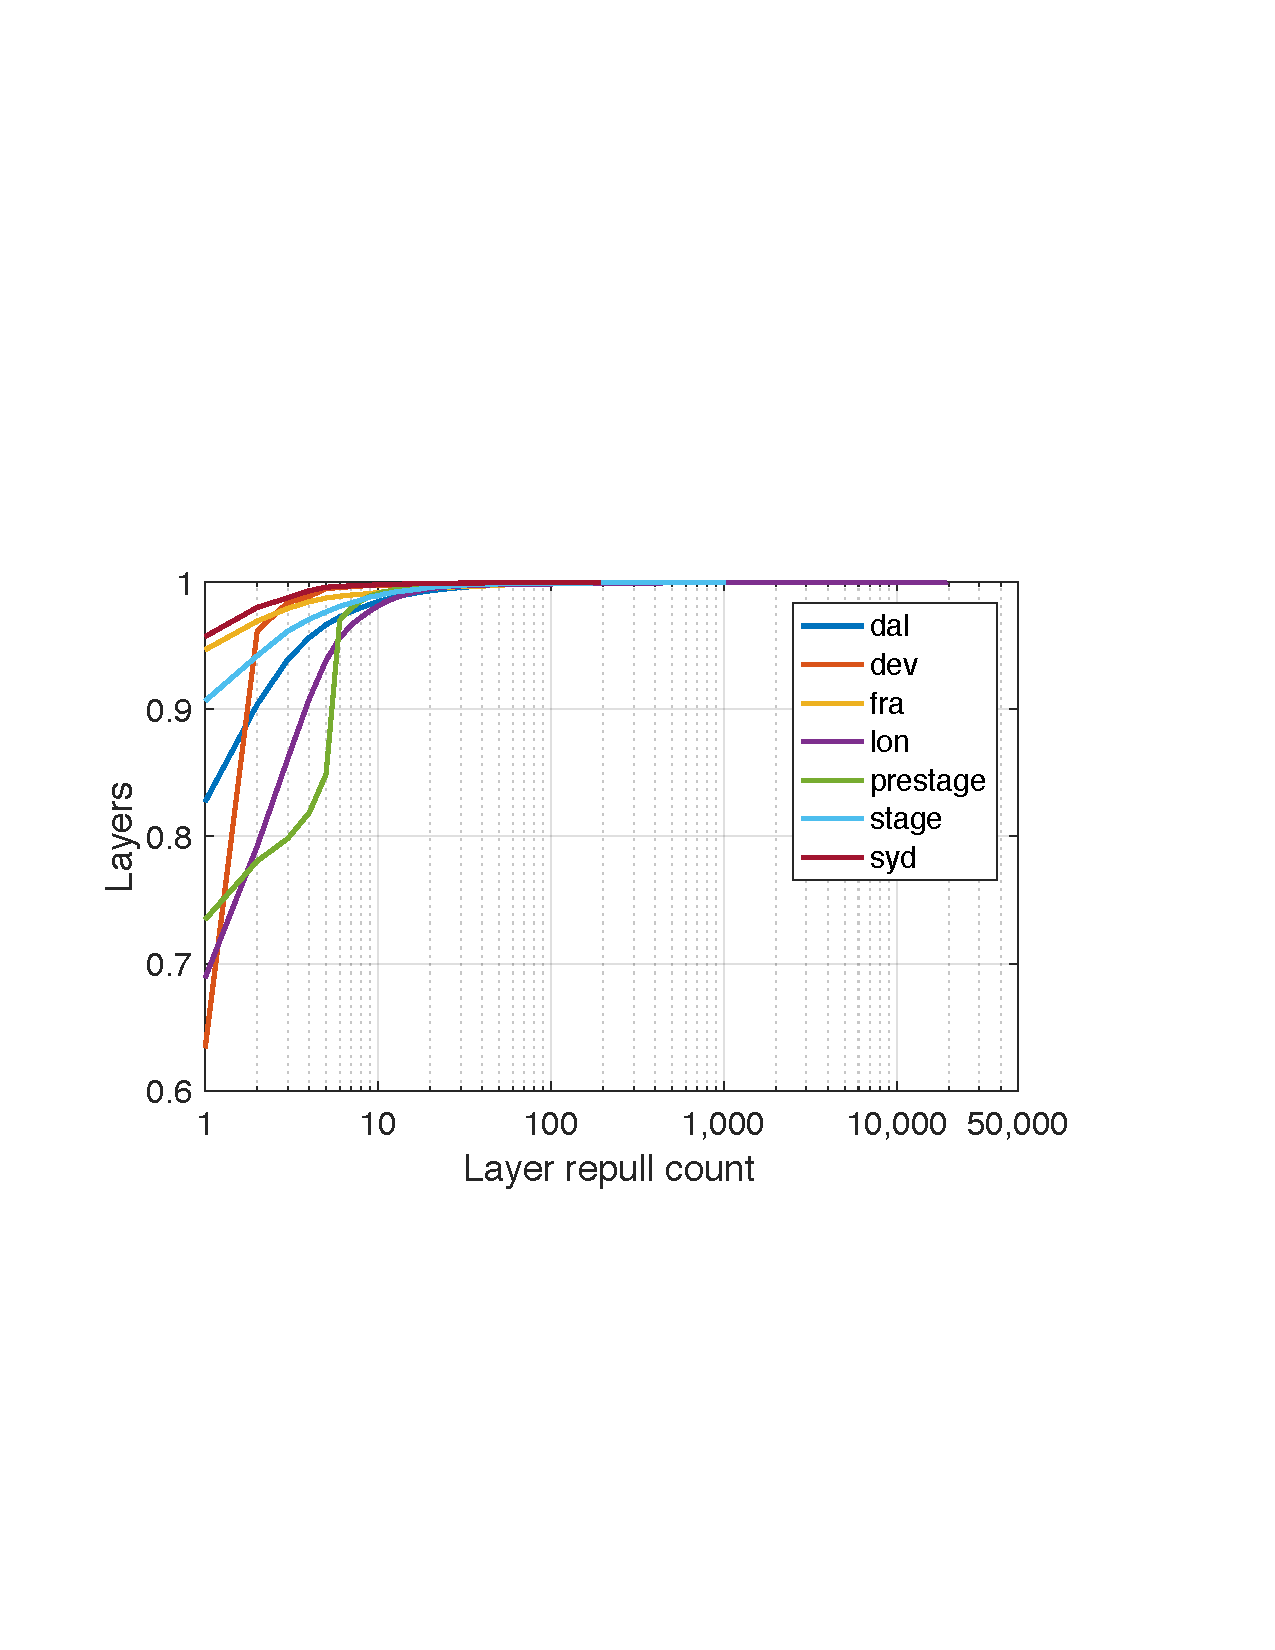
\includegraphics[width=1\textwidth]{graphs/cdf-layer-repull-by-same-client.pdf}
%			%\caption{CDF of layer repull count.}
%		%	\vspace{-3pt}
%			\label{fig:layer-repull-cdf}
%		\end{minipage}
%			\begin{minipage}{0.32\linewidth}
%				\centering
%				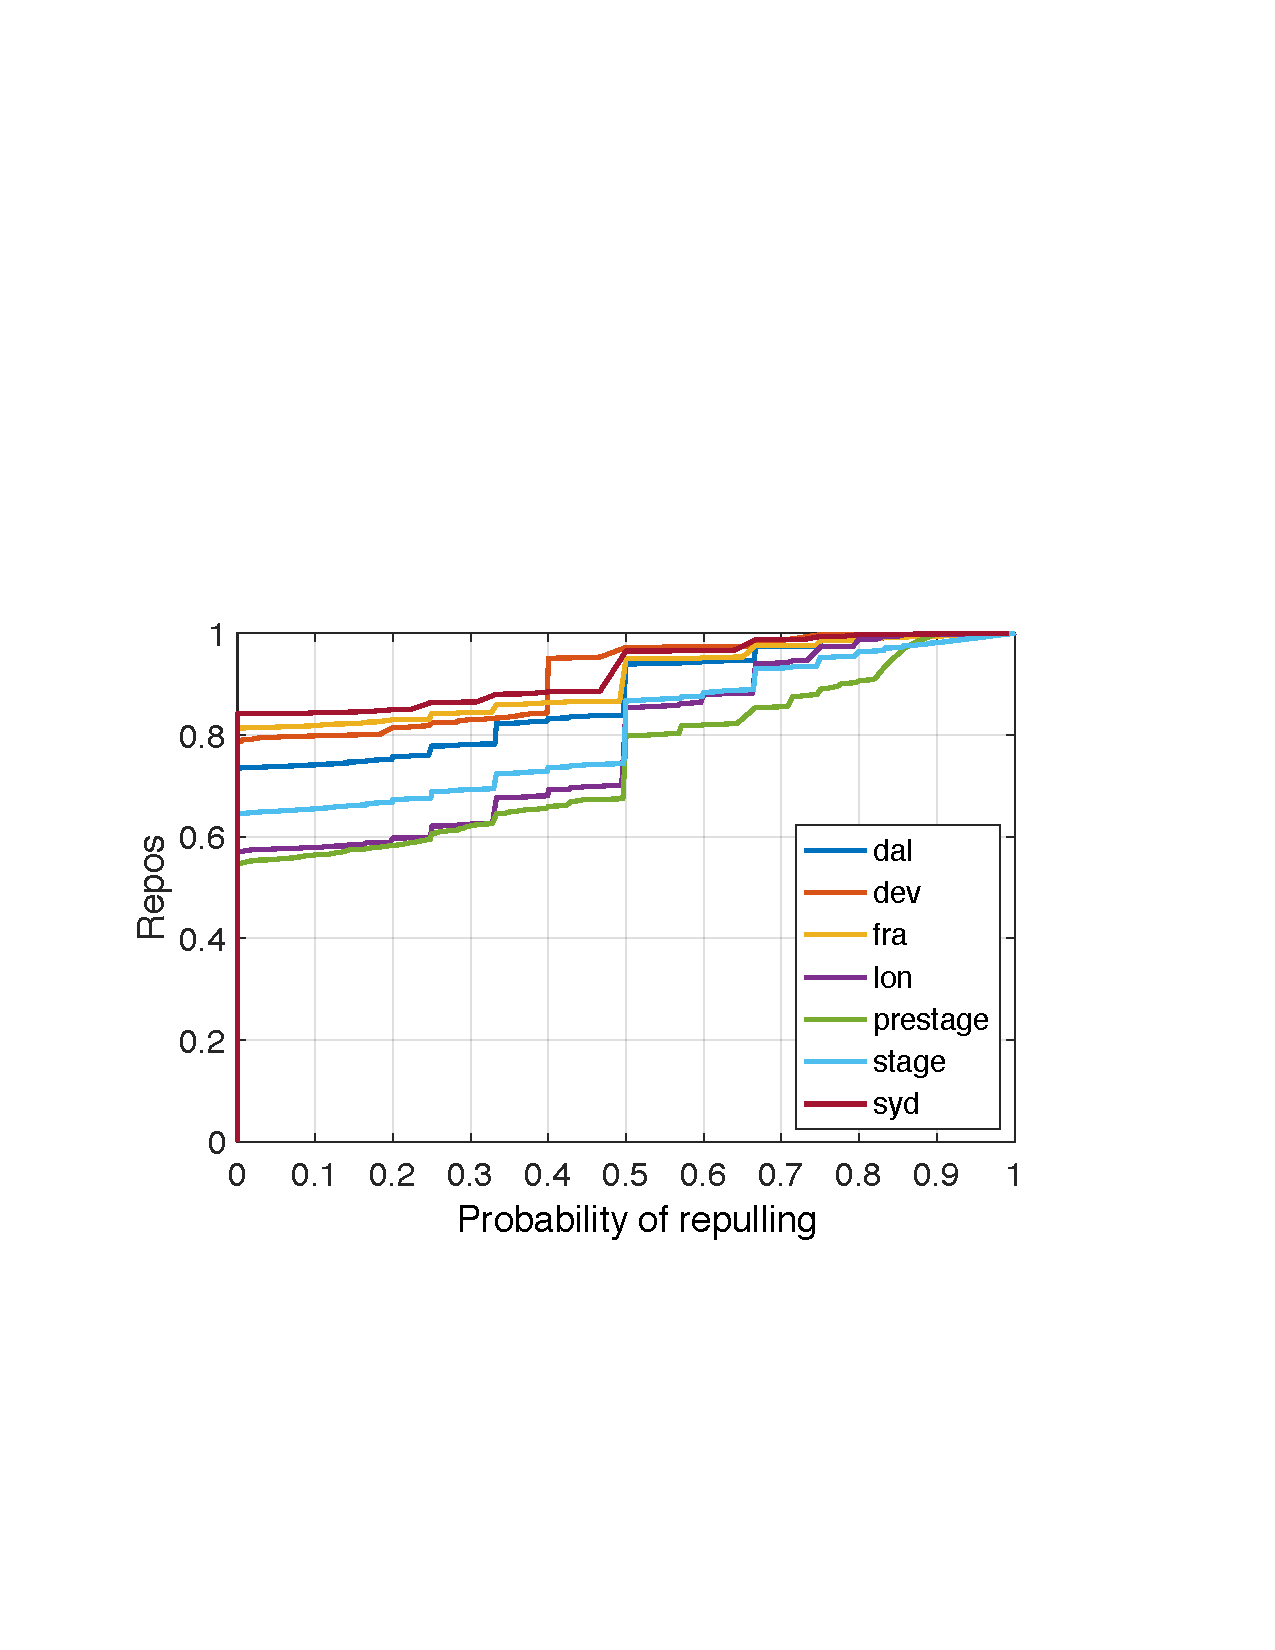
\includegraphics[width=1\textwidth]{graphs/cdf-repo-repull-ratio-by-same-client.pdf}
%				%\caption{PDF of repository repulling probability.}
%				%	\vspace{-3pt}
%				\label{fig:repo-repull-cdf}
%			\end{minipage}
%		\begin{minipage}{0.32\linewidth}
%			\centering
%			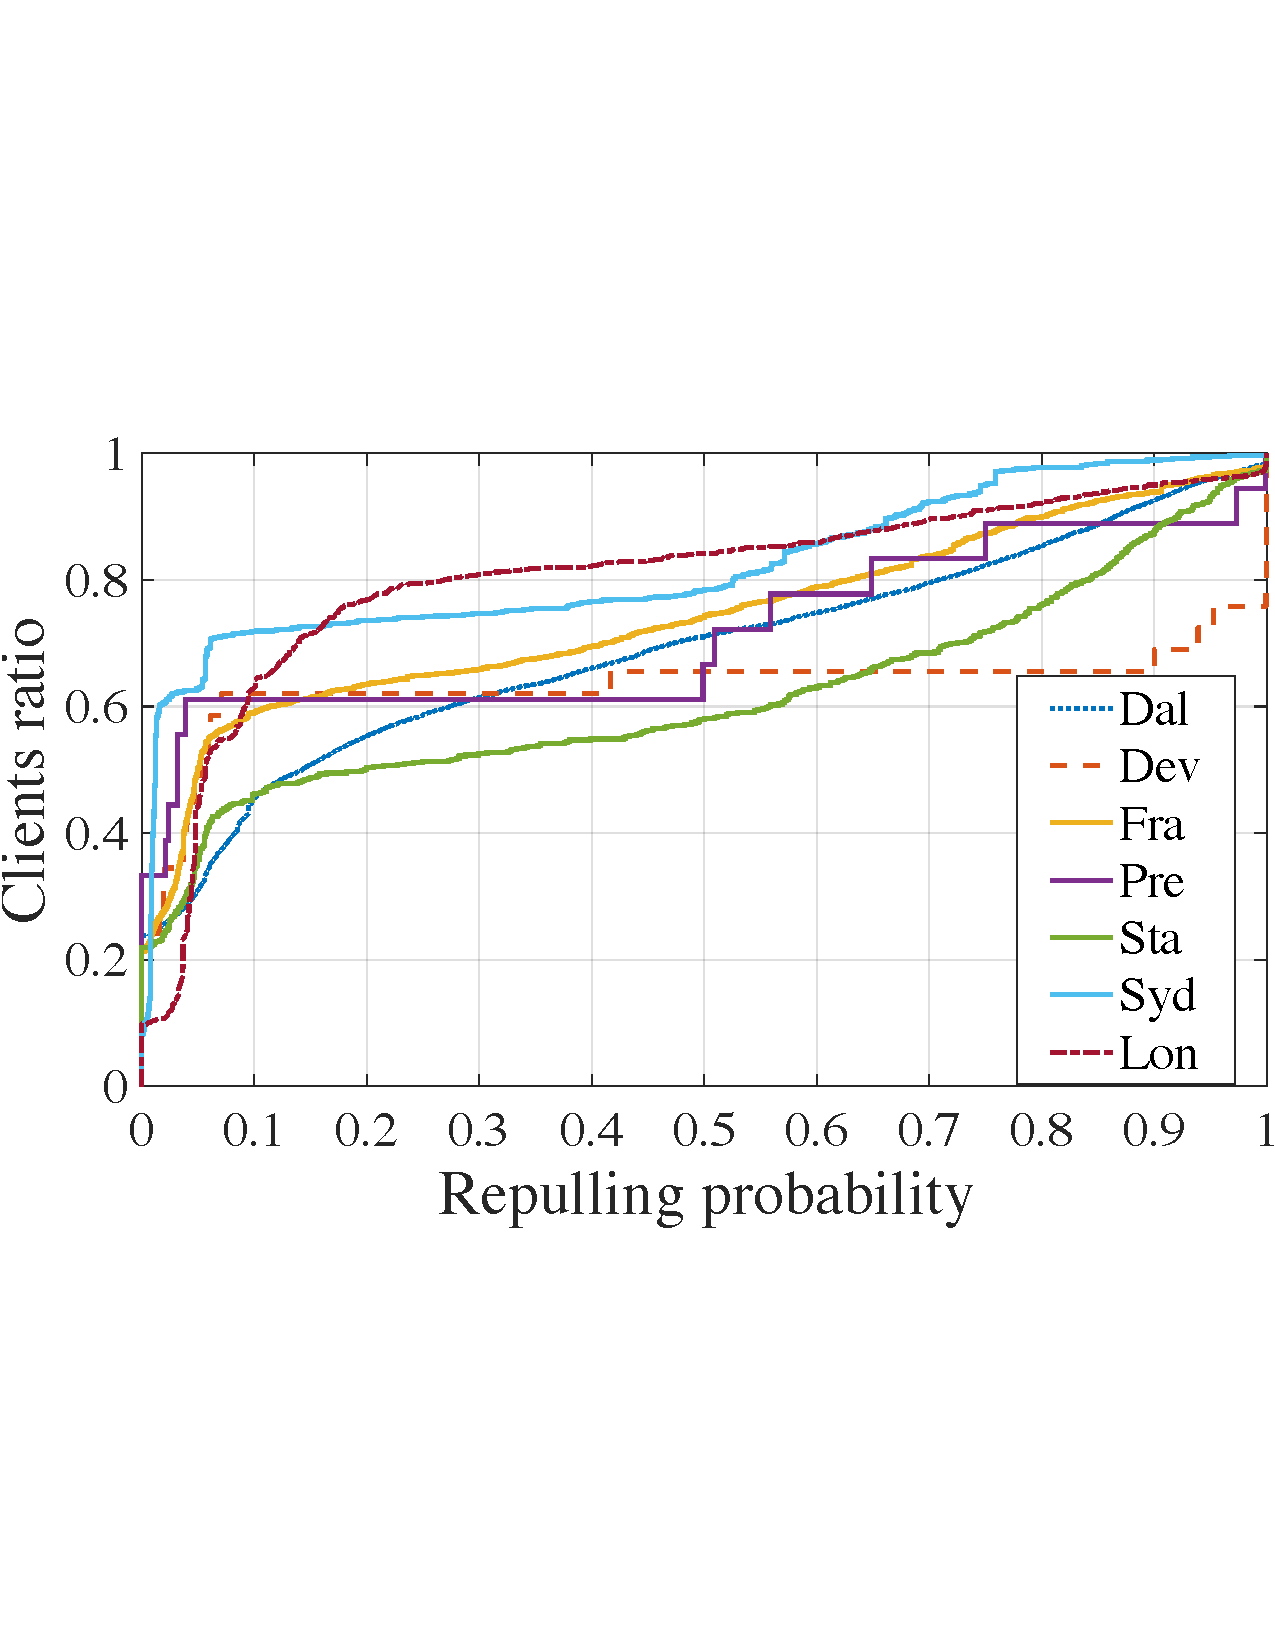
\includegraphics[width=1\textwidth]{graphs/cdf-client-repull-layer-request-ratio.pdf}
%			%
%			%	\vspace{-3pt}
%			\label{fig:client-repull-cdf}
%		\end{minipage}
%	\caption{PDF of client repull count, repository repulling probability, and client repulling probability..}
%\end{figure*}

%\begin{figure}[!t]
%	\centering
%	\subfigure[\texttt{GET} layer request count]{
%		\includegraphics[width=0.22\textwidth]{graphs/cdf-layer-repull-ratio-by-same-client.pdf}
%		\label{fig:layer-repull-cdf}
%	}
%%	\subfigure[Repository repulling probability]{
%%		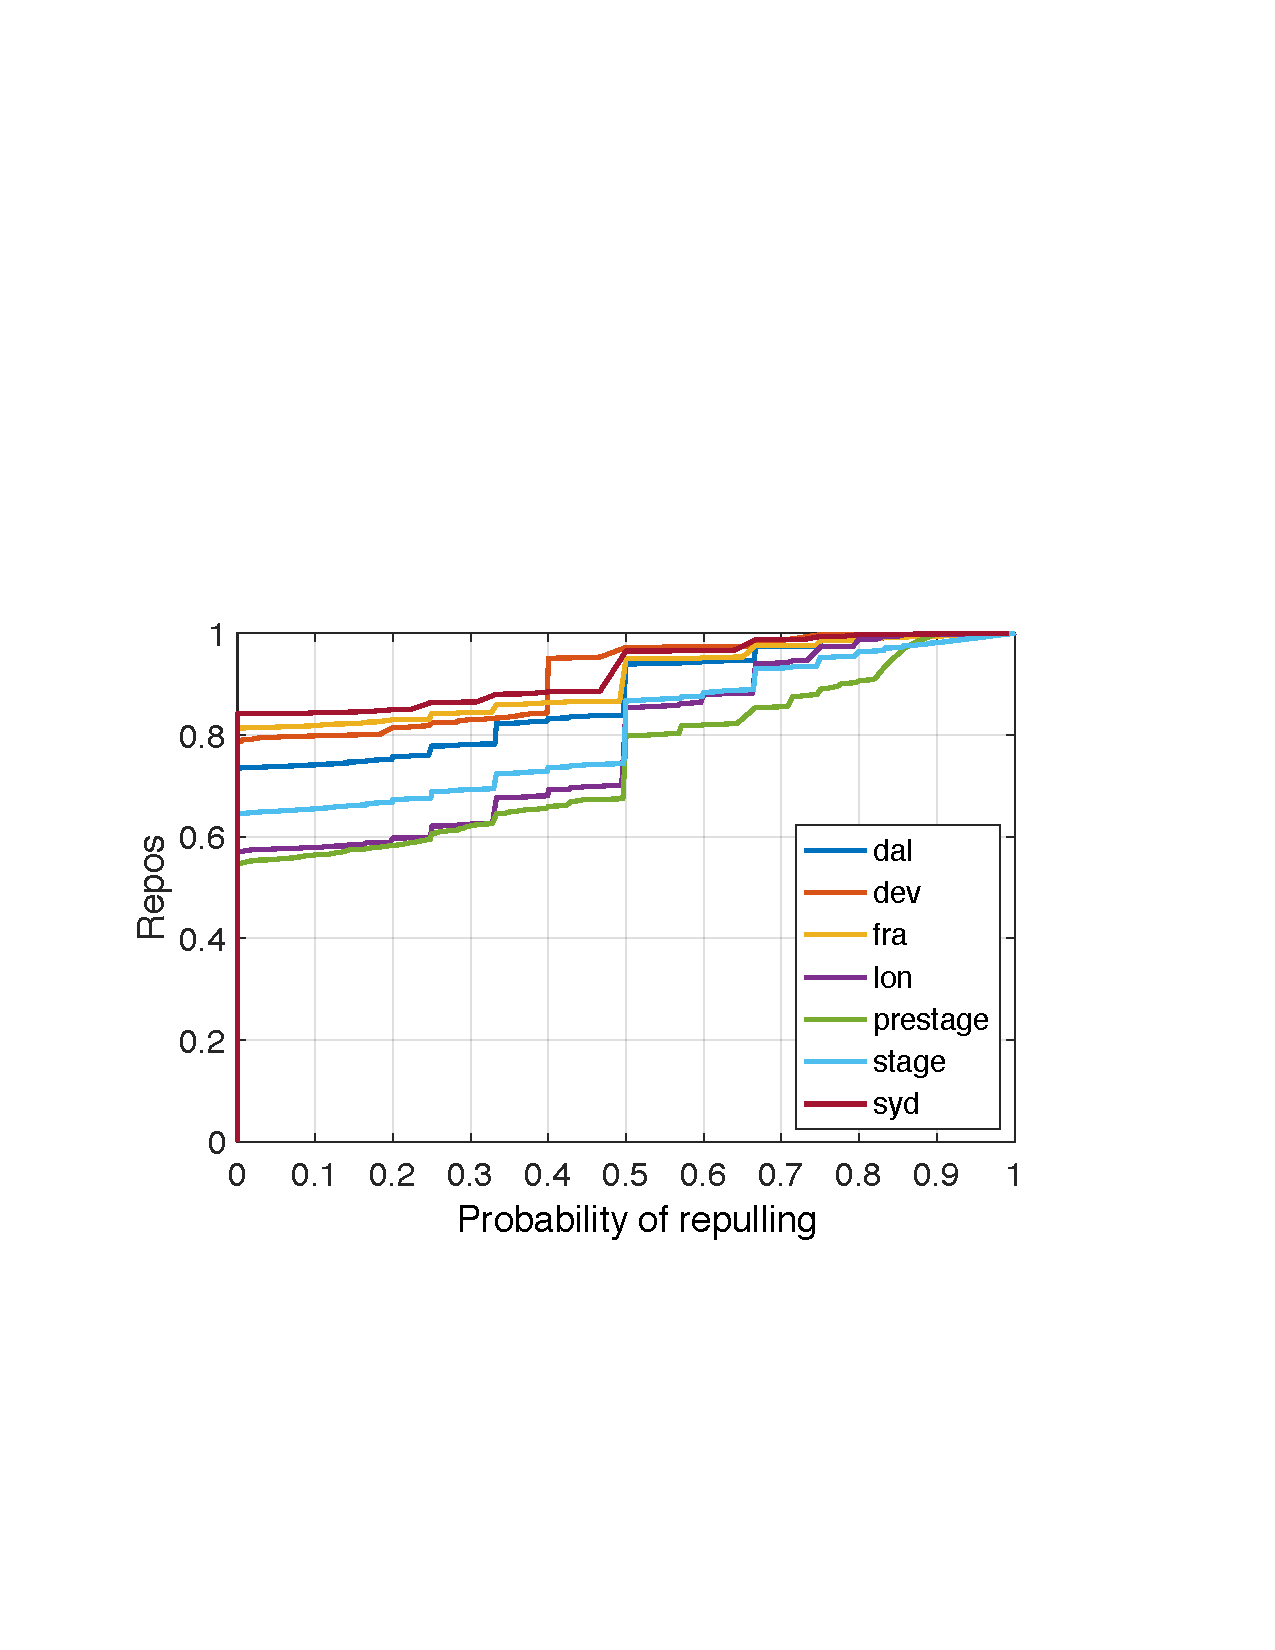
\includegraphics[width=0.2\linewidth]{graphs/cdf-repo-repull-ratio-by-same-client.pdf}
%%		\label{fig:repo-repull-cdf}
%%	}
%	\subfigure[Client repulling probability]{
%	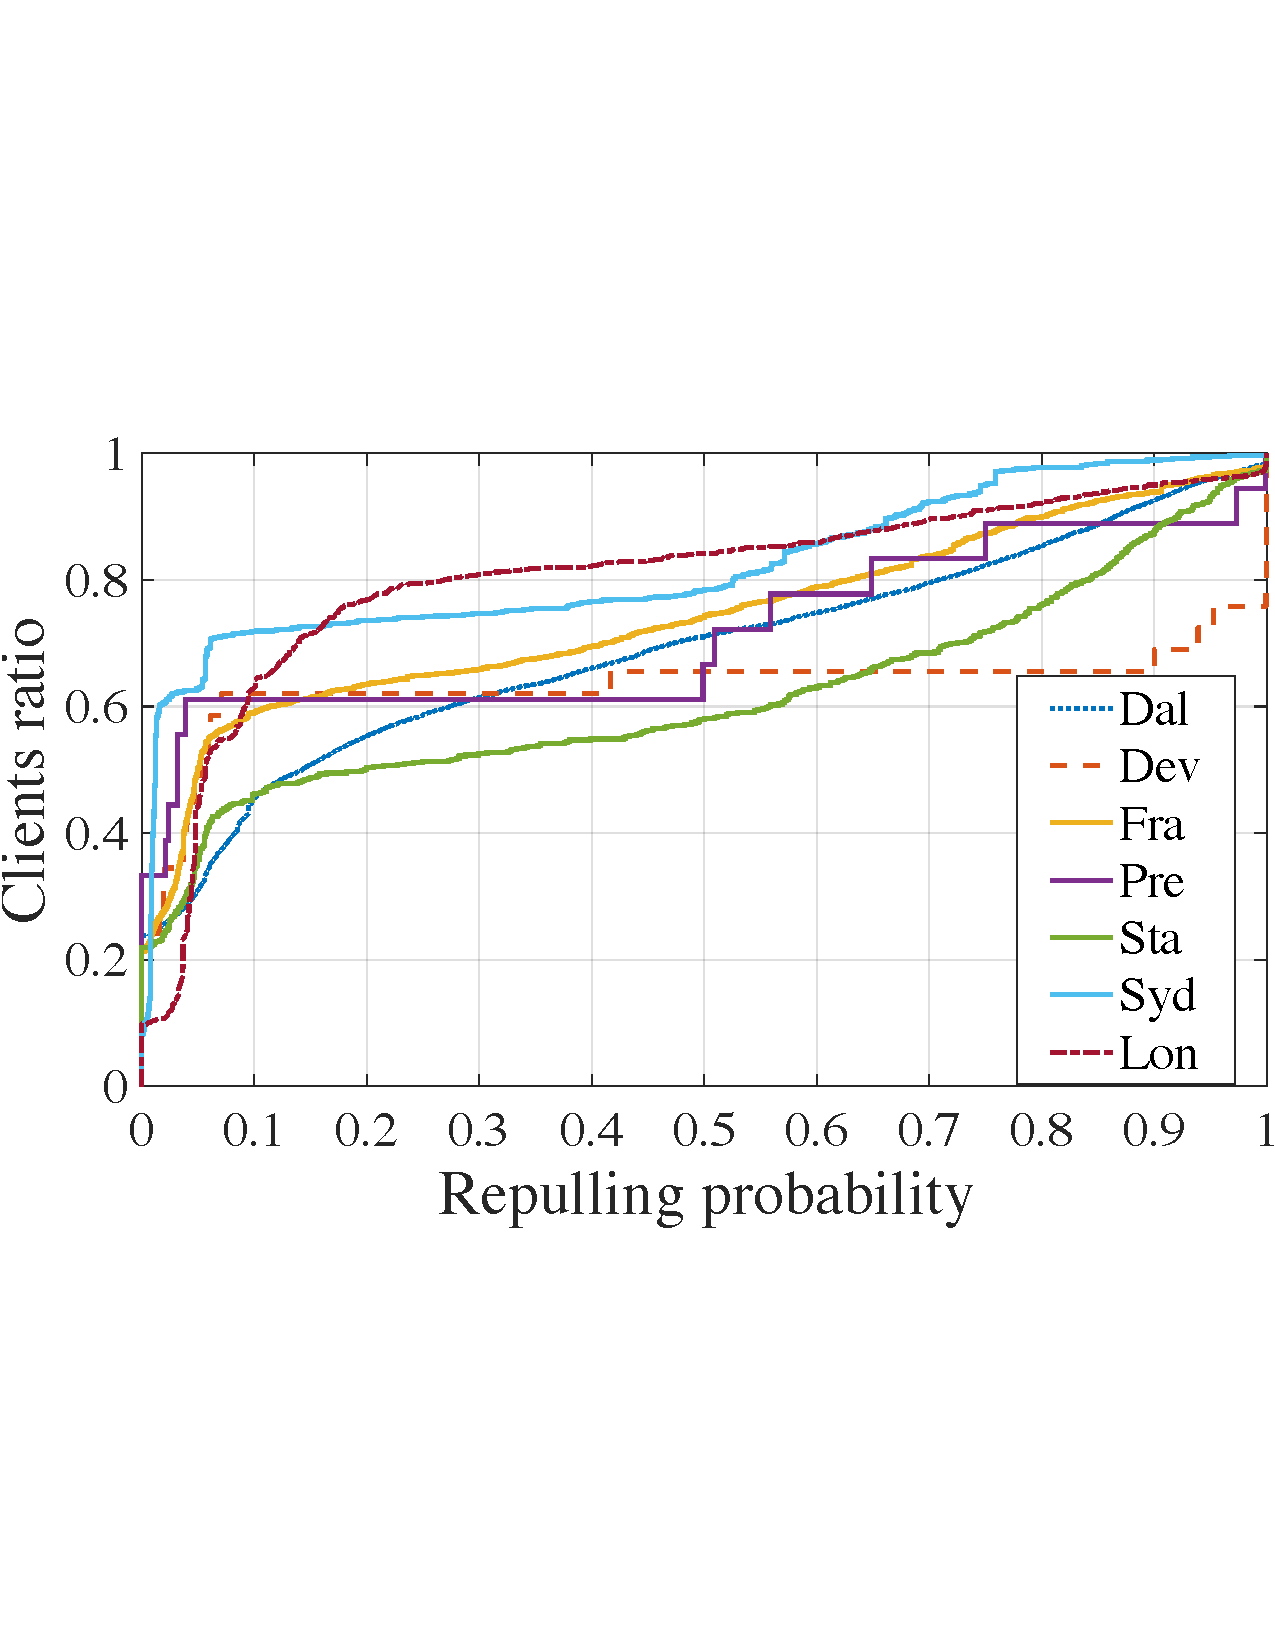
\includegraphics[width=0.2\textwidth]{graphs/cdf-client-repull-layer-request-ratio.pdf}
%   \label{fig:client-repull-cdf}
%}
%	\caption{CDF of \texttt{GET} layer request count and client repulling probability.}
%	\label{fig-repull}
%\end{figure}
%






\begin{figure*}[t]
        \centering
        \begin{minipage}{0.3\textwidth}
                \centering
                \includegraphics[width=0.9\textwidth]{{graphs/cdf-layer-repull-ratio-by-same-client.pdf}
                \caption{CDF of \texttt{GET} layer request count}
                \label{fig:layer-repull-cdf}
        \end{minipage}%
        \begin{minipage}{0.3\textwidth}
                \centering
                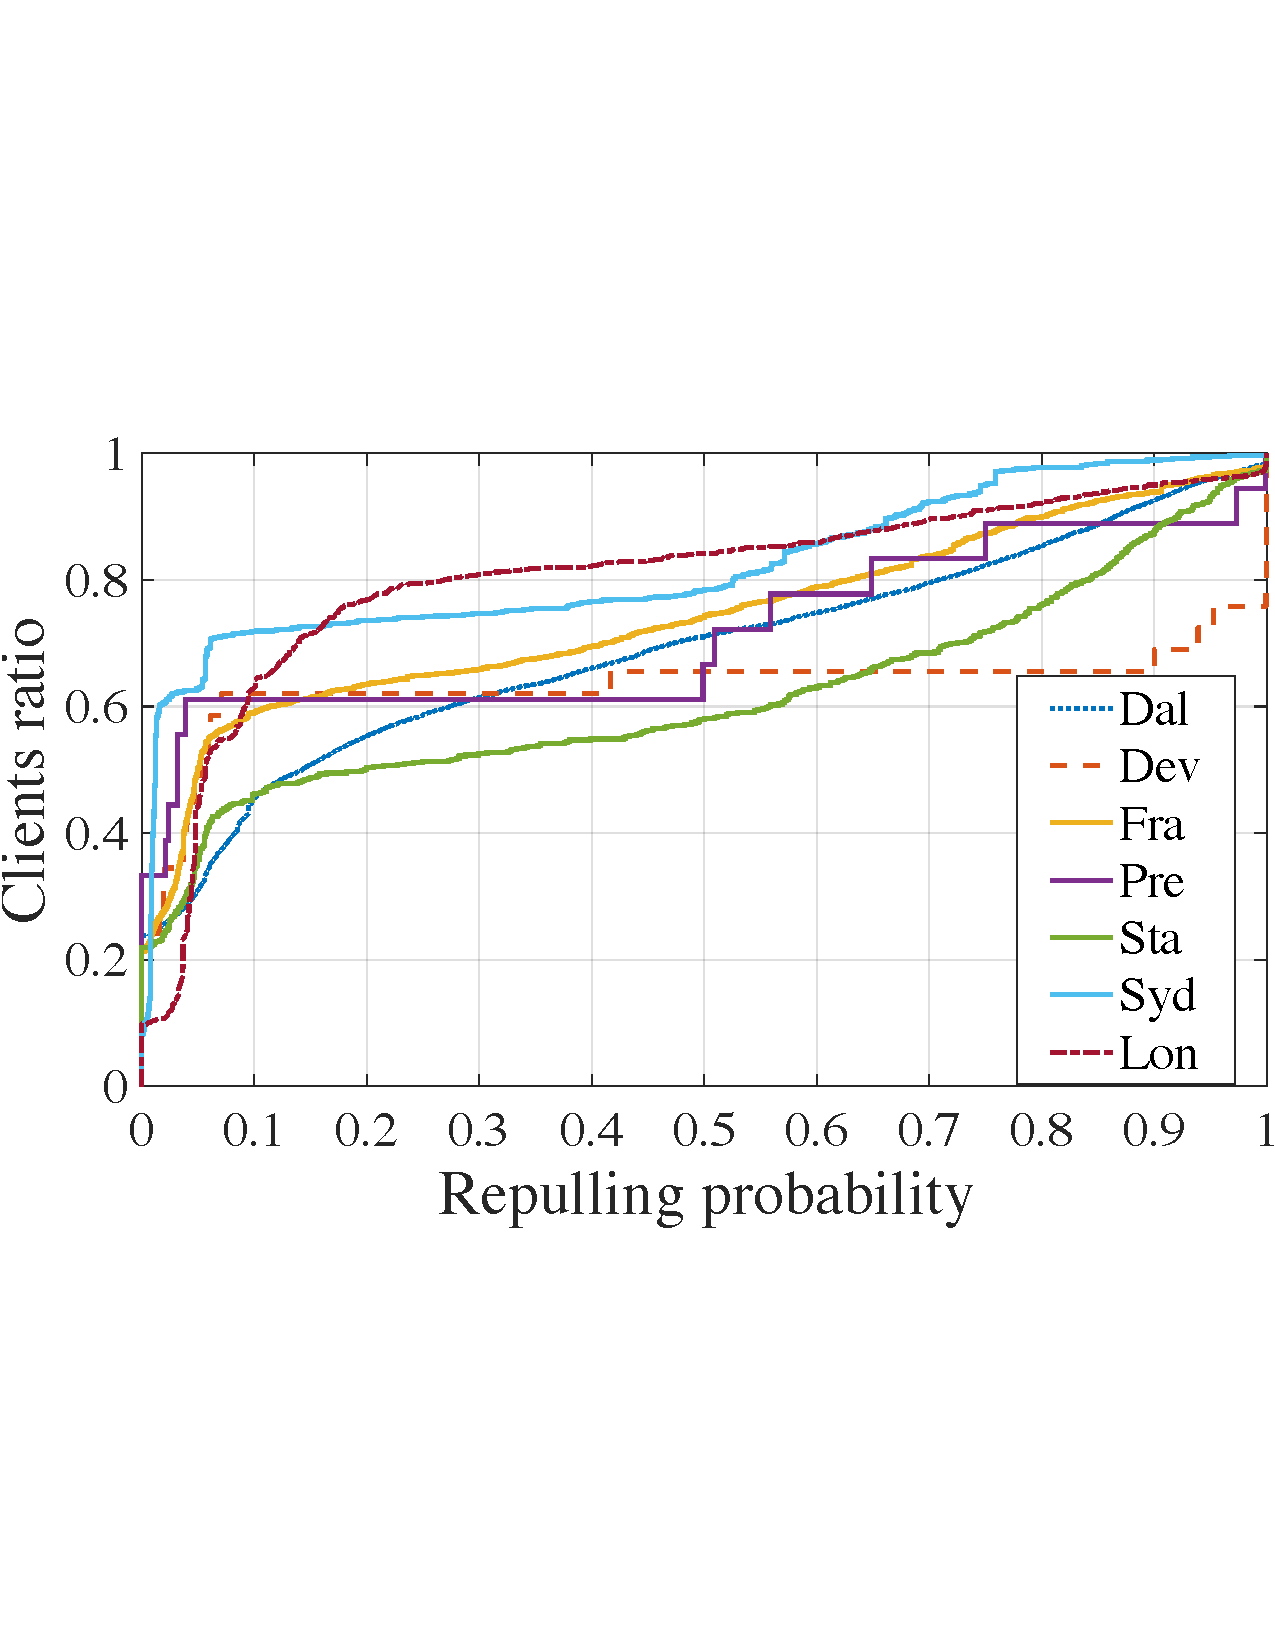
\includegraphics[width=0.9\textwidth]{graphs/cdf-client-repull-layer-request-ratio.pdf}
                \caption{CDF of Client repulling probability}% of LRU cache and preconstruct cache.}
                \label{fig:client-repull-cdf}
        \end{minipage}%
        \begin{minipage}{0.3\textwidth}
        \centering
        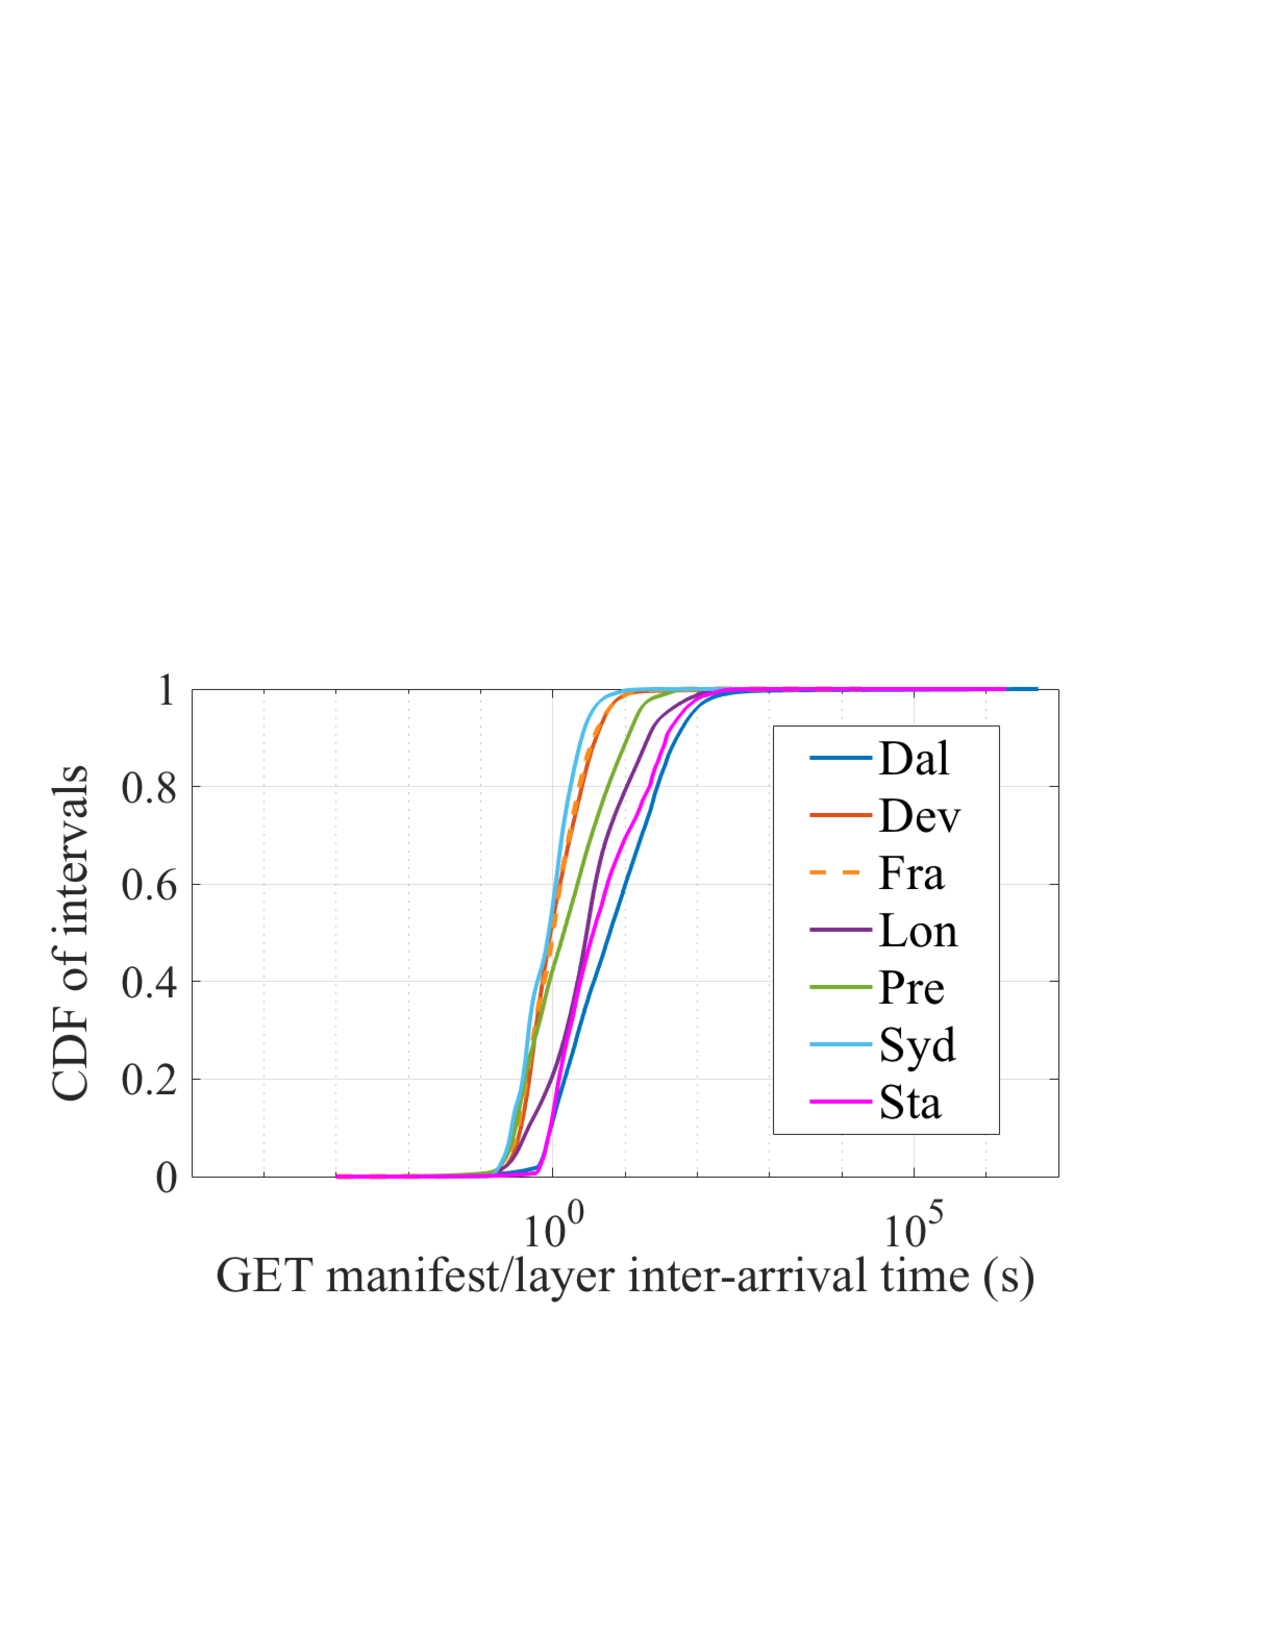
\includegraphics[width=0.9\textwidth]{graphs/GML-intervals.pdf}
        \caption{Intervals between \texttt{GET} manifest request and \texttt{GET} layer request}
        \label{fig:intervals}
   \end{minipage}
\end{figure*}





%\begin{figure}[!t]
%	\centering
%	\subfigure[CDF of compression ratio]{\label{fig_cdf_compression_ratio}
%		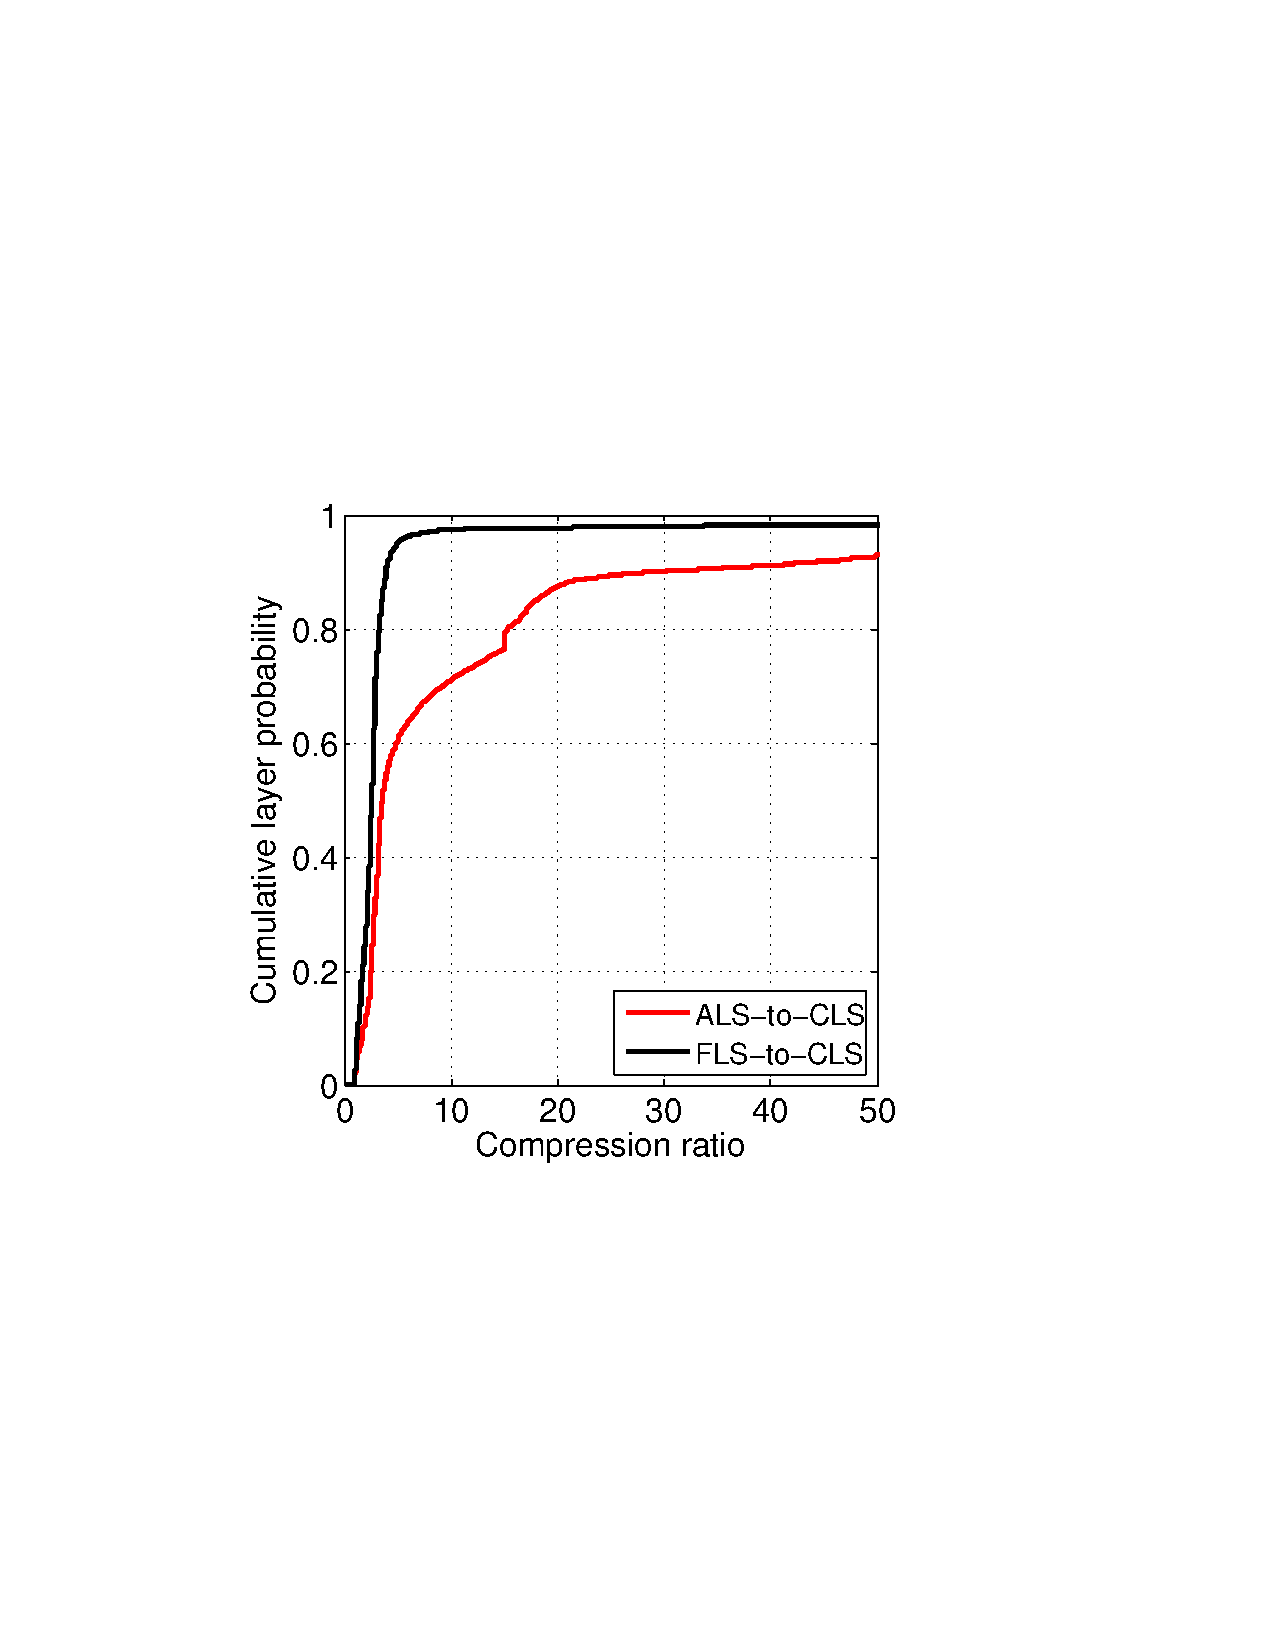
\includegraphics[width=0.23\textwidth]{graphs/cdf_compression_ratio.pdf}
%	}
%	\subfigure[Histogram of comp. ratios]{\label{fig_his_compression_ratio}
%		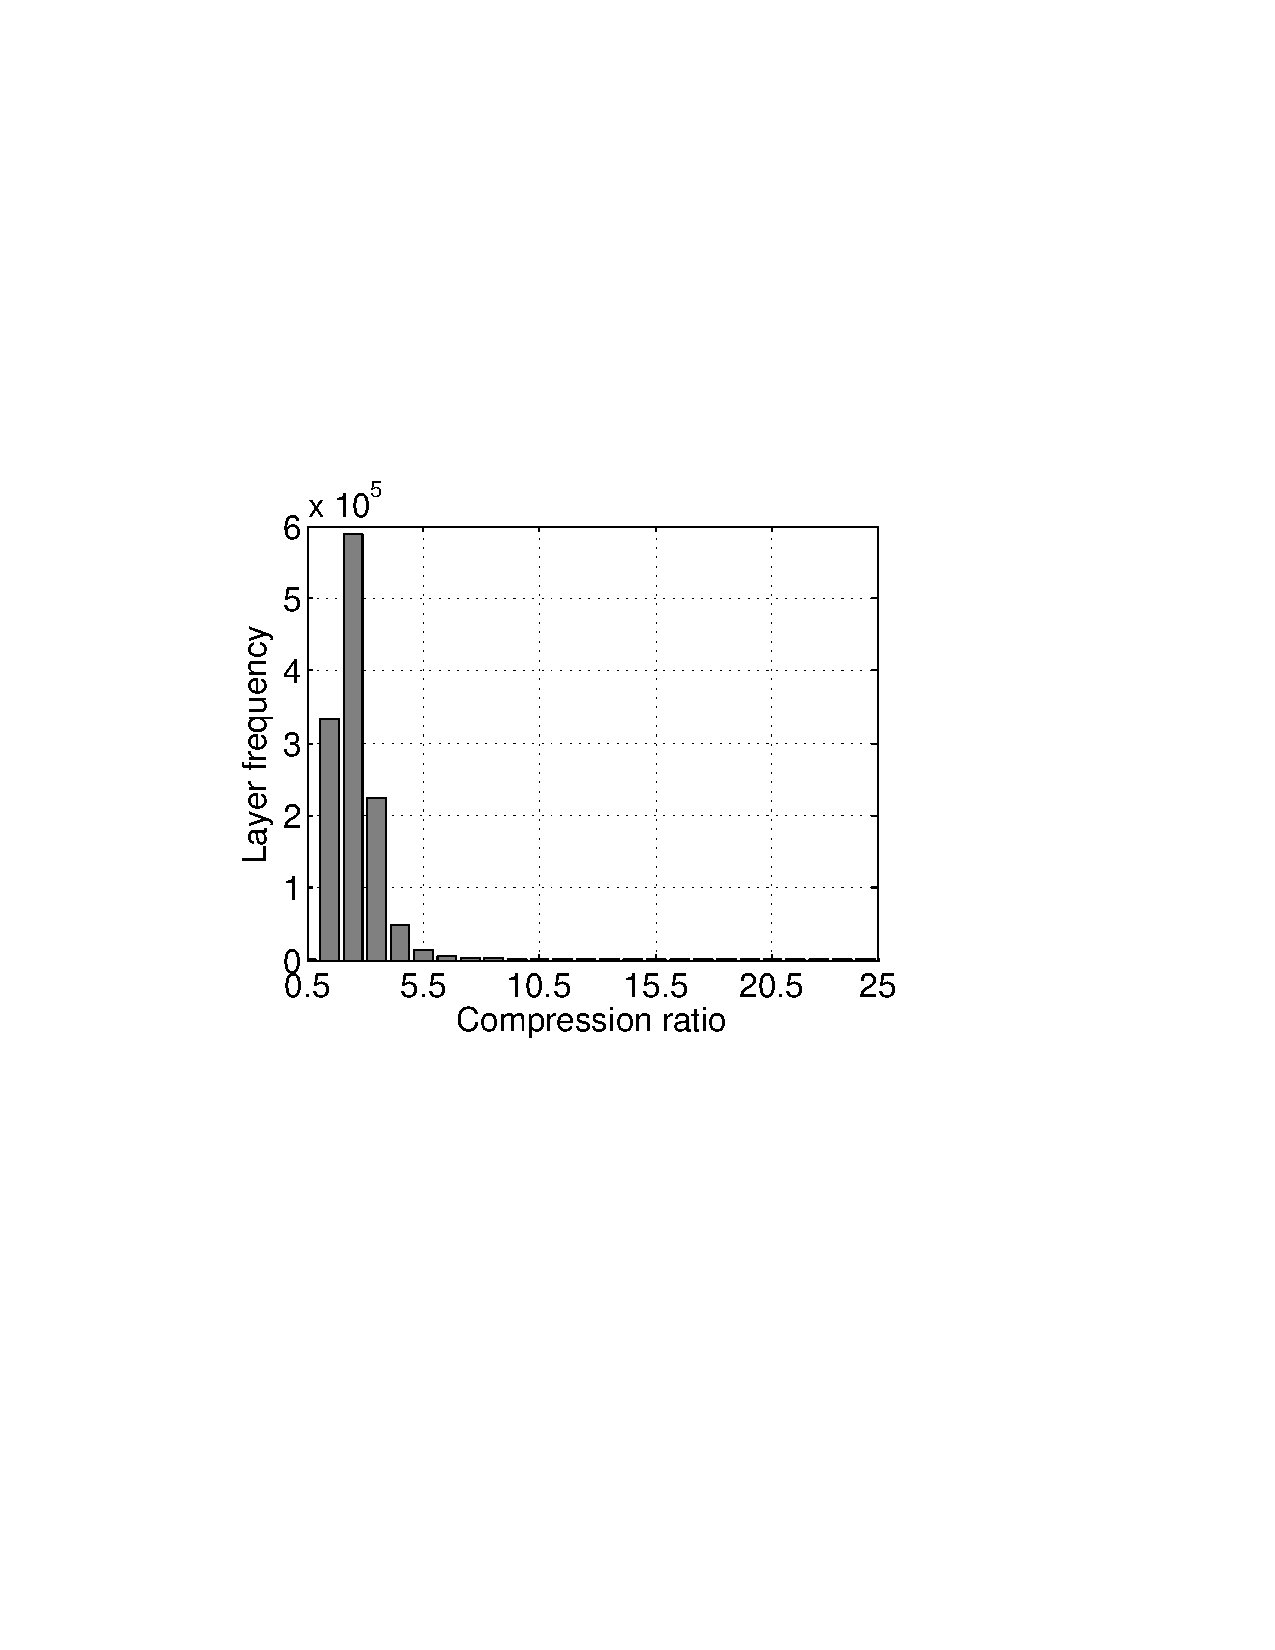
\includegraphics[width=0.223\textwidth]{graphs/his_compression_ratio.pdf}
%	}
%	\caption{Layer compression ratio distribution
%		%\vcomment{Different colors are used in figure (a) and (b) FLS/CLS\nancomment{will address later}}
%	}
%	\label{fig-compression-ratio}
%\end{figure}


%\begin{figure}[t]
%	\centering
%	\begin{minipage}{0.26\textwidth}
%		\centering
%		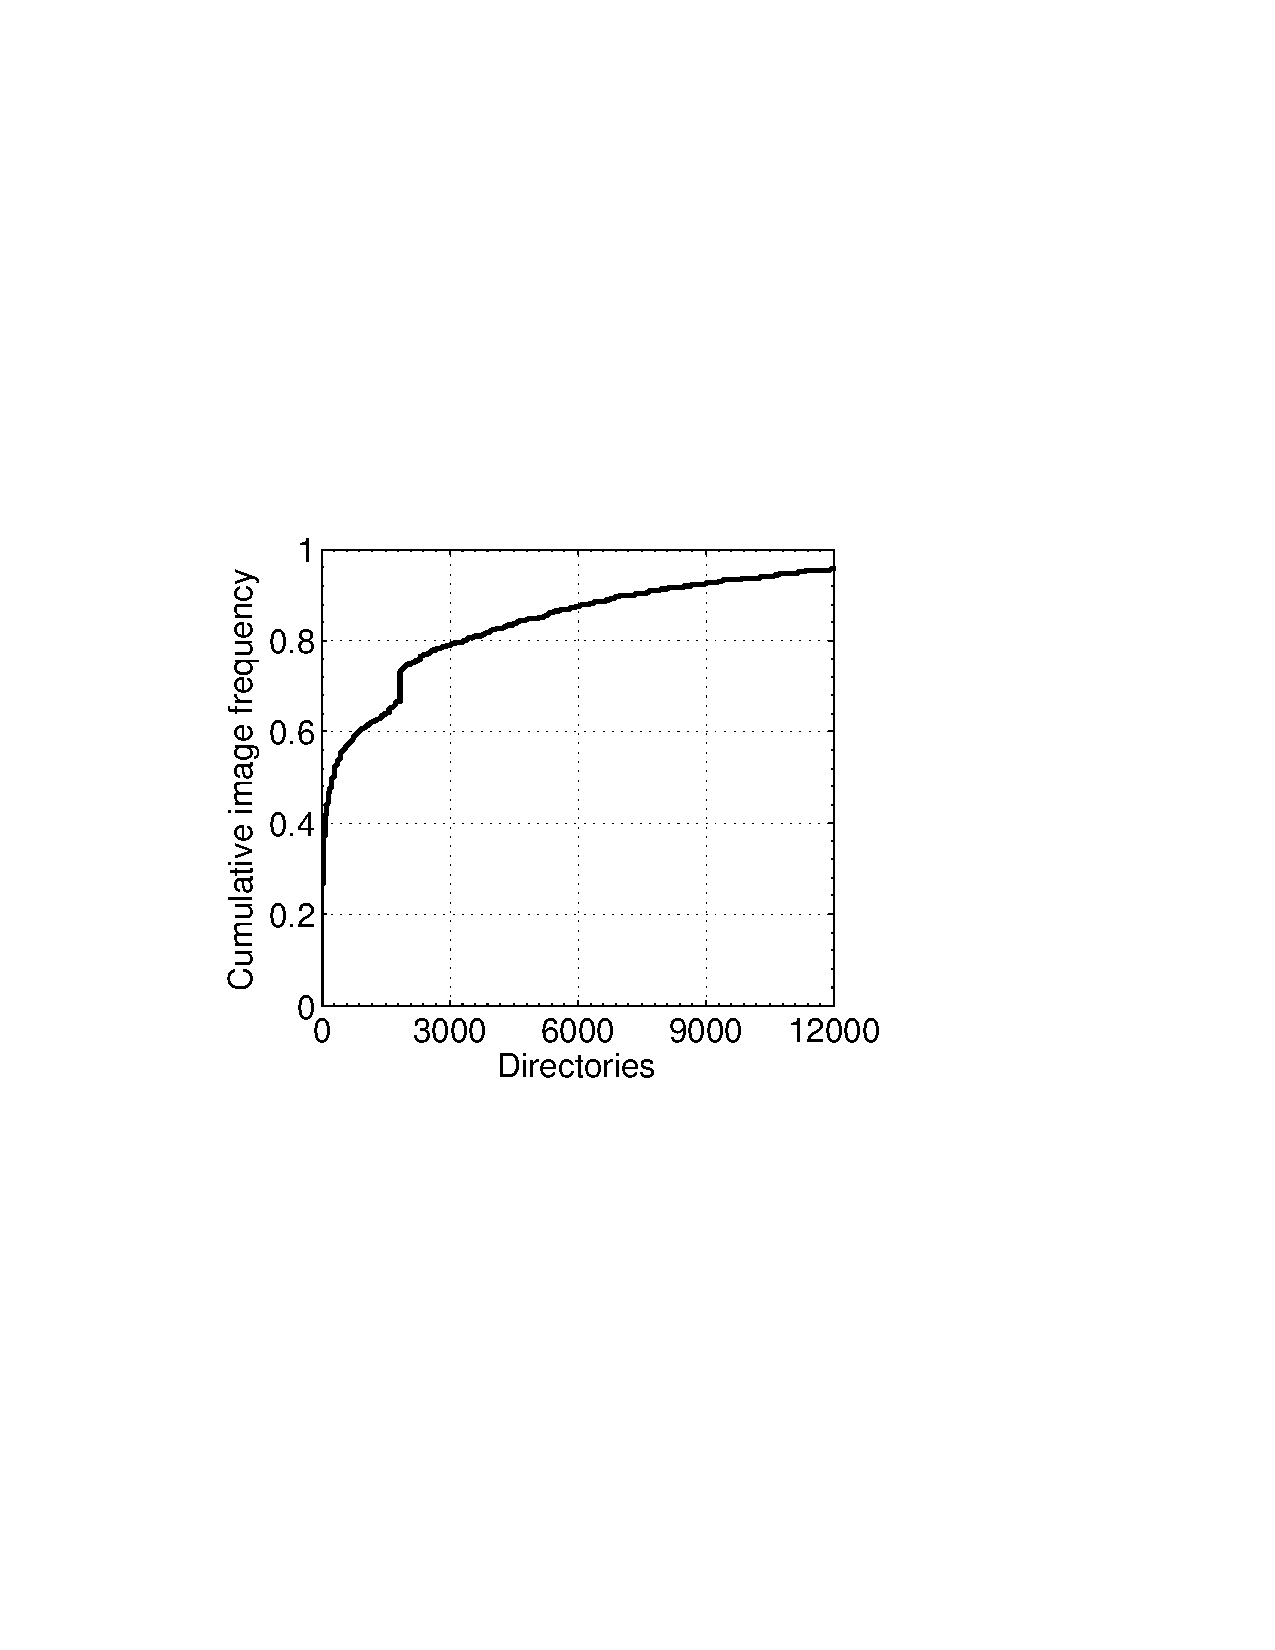
\includegraphics[width=1\textwidth]{graphs/dir.pdf}
%		\caption{CDF of images by\newline directories}
%		\label{fig-dir}
%	\end{minipage}%
%	\begin{minipage}{0.24\textwidth}
%		\centering
%		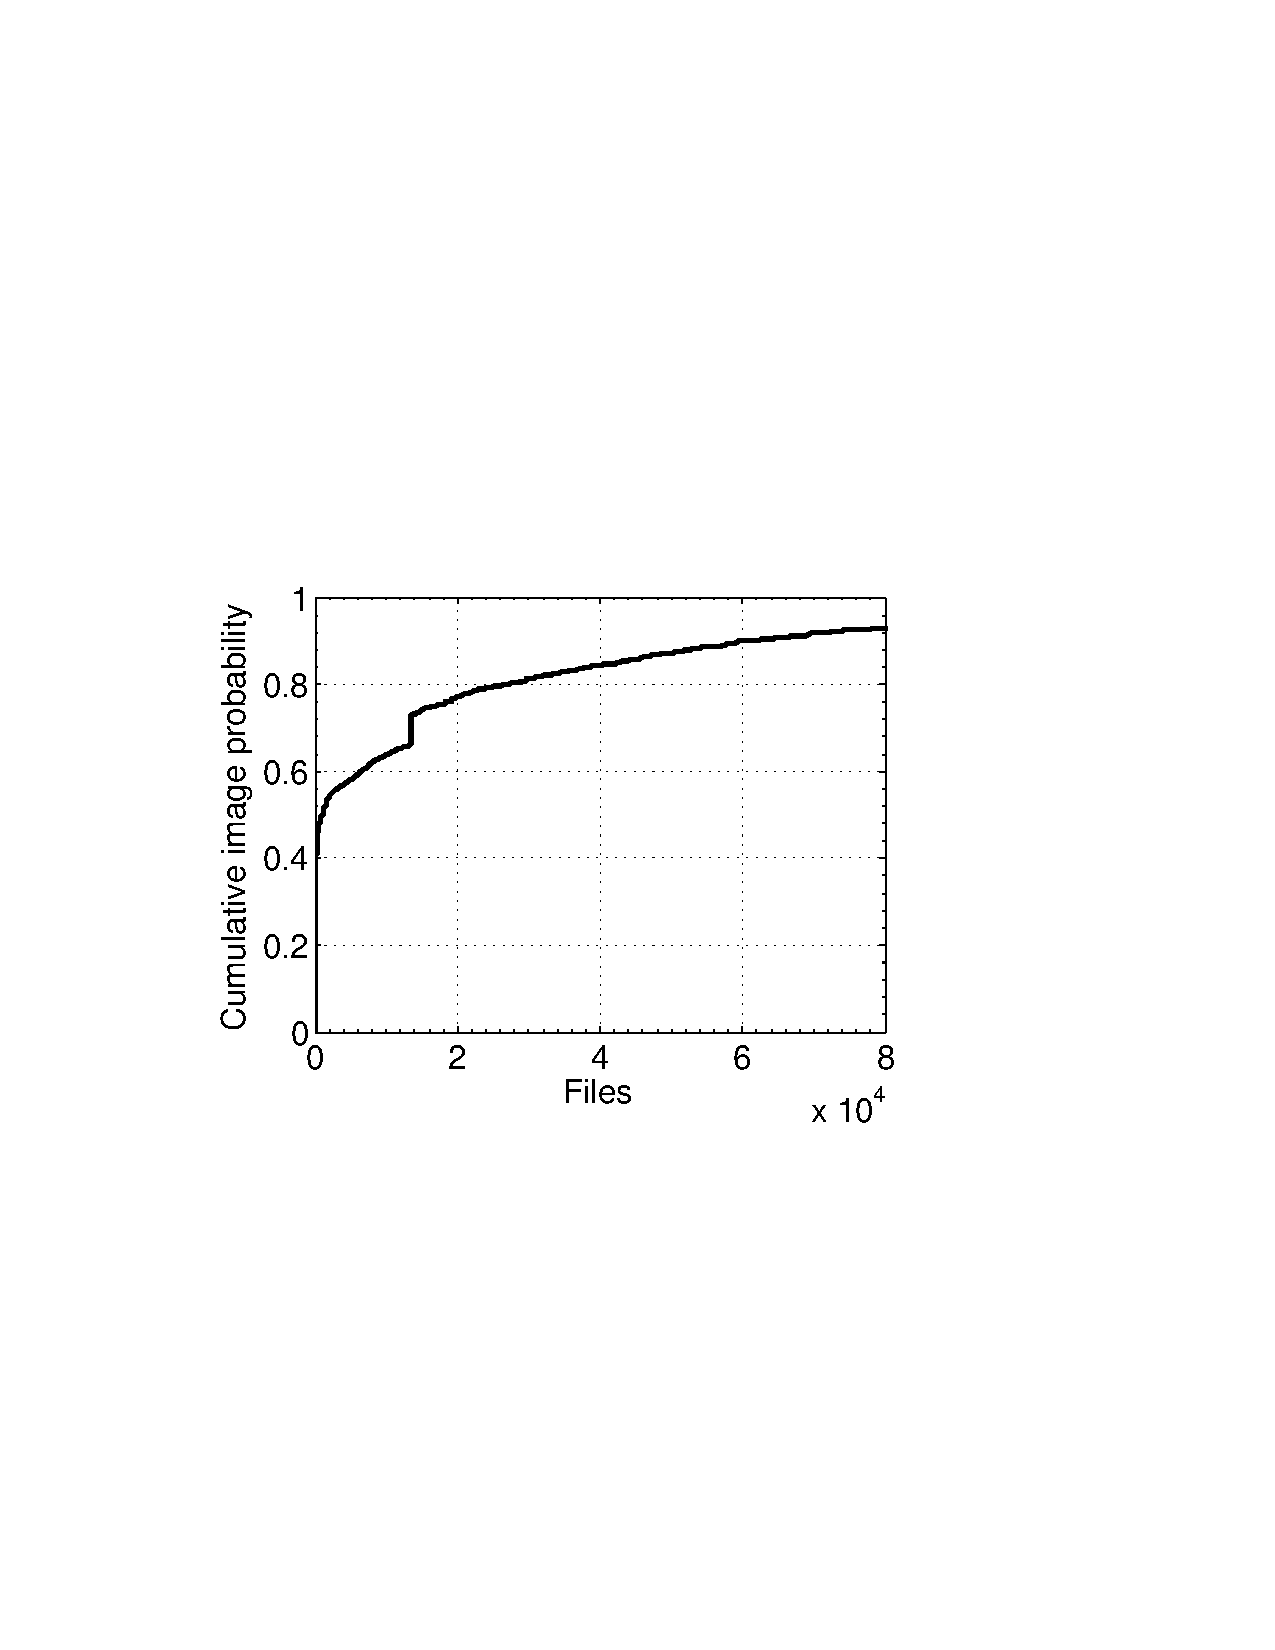
\includegraphics[width=1\textwidth]{graphs/file.pdf}
%		\caption{CDF of images by files}
%		\label{fig-file}
%	\end{minipage}
%\end{figure}

%\begin{figure}[htbp] 
%	\begin{minipage}{0.5\linewidth} 
%		\centering 
%		\includegraphics{circle} 
%		\caption{A Circle} 
%		\label{fig:circle} 
%	\end{minipage}% 
%	\begin{minipage}{0.5\linewidth} 
%		\centering 
%		\includegraphics{rectangle} 
%		\caption{A Rectangle} 
%		\label{fig:rectangle} 
%	\end{minipage} 
%\end{figure}


%<<<<<<< HEAD
\paragraph{User access patterns} 
When a Docker client \texttt{pulles} an image from Docker registry,
it will first \texttt{pull} the \textbf{manifest} of the image, 
which is metadata file of the image and contains a list of layers' digests.
After that, the client parses the manifest, gets a list of layers referenced by the image,
and compares against a \emph{local layer index}.
If a layer doesn't exist in the local layer index,
 the client will \texttt{pull} this layer.
 Thus, we can maintain a \emph{user local layer index} on registry side to keep track of user access history
 and predict which layer will be \texttt{pulled} by the user when the user issues a \texttt{pulling} manifest request.

Typically, if a layer is already stored locally,
then the client will not \texttt{pull} this layer again.
However, for Kubernetes,
users can configure different \emph{pull policies}, 
such as \emph{IfNotPresent (i.e, pulling if not present)} or \emph{Always pulling}.
We observe these two kinds of user behaviors in the real world workloads~\cite{xxx} as follows:
%we observe that few clients pull the same layers multiple time

\paragraph{Pull once VS. Always pull}
Figure~\ref{fig:layer-repull-cdf} shows the CDF of layer \texttt{pull} count by the same clients. 
%Here, \emph{repulling} indicates the act of pulling layers that have been pulled by the user before because they are no longer present on the user side.
Majority of layers are only pulled once by the same clients.
%83\% of the layers are only pulled twice.
For example, only 97\% of layers from \texttt{Syd} are only pulled once by the same clients.
We also observe that few clients \emph{pull} the same layers continuously.
For example, a client from \texttt{Lon} pulls the same layer 19,300 times.
%When different clients \texttt{pull} the same repository, 
%they will fetch different amount of layers from the repository based on the contents of their local layer dataset. 
%The local layers can vary with time due to clearing of the data so the same clients can fetch different amounts of layers at different times.
%Therefore, a \texttt{pull manifest} request doesn't usually result in repulling all the layers in the repository. 
%Here, we define \emph{repulling a repository} as repulling the layers in the repository for the same client.
%Figure~\ref{fig:repo-repull-cdf} shows the CDF of the probability of repository repulling, calculated 
%as the number of \texttt{pull manifest} resulting in repository repulling divided by 
%the total number of \texttt{pull manifest} requests issued for the same repository.
%We see that majority of repositories aren't repulled.
%The percentage of repositories whose repull probability is zero (i.e. are pulled only once by a client) ranges from 57\% for \texttt{Prestage} to 85\% for \texttt{Syd}.
%Only 20\% of repositories from  \texttt{Prestage}, \texttt{Stage}, and 
%\texttt{Syd} have a repulling probability higher than 0.5.
%We also observe that few repositories' repulling probability is 1, indicating repulls everytime by the clients.

We define \emph{repulling} as the act of pulling the same layer more than once by the same user.
% before because they are no longer present on the user side.
Figure~\ref{fig:client-repull-cdf} shows the client repulling probability, calculated as the number of \emph{repulling} layer requests divided by
the number of total \texttt{pull} layer requests issued by the same client.
We see that a significant amount of clients have a low repulling proability.
For example,
71\% of clients from \texttt{syd} have a repulling probability lower than 0.1.
Very few clients have a high repulling probability.
For instance,
only 2\% clients have a repulling probability higher than 0.9 from 
\texttt{Dal}.

We also observe that the slope is steep at both lower and higher probabilities.
But the slope becomes gentle in the middle.
For example, 
the slope at probabilities between 0.1 and 0.9 for \texttt{dev} almost equals to zero.
In this case,
the high repulling probability clients can be classified as always-pull clients, 
and the low repulling probability clients as pull-once clients. 
The few clients in the middle are considered as \emph{erratic}.
%
Thus,
to determine whether a client will \texttt{repull} a layer or not,
we consider the client repulling probability and the layer repull count.
%From the probability distribution of the clients repulling, we can observe that a significant chunk of the clients have very low repulling probability and another chunk of the clients have a very high repulling probability, with few clients in the middle. For simplicity of implementation, the high probability clients can be classified as always repulling clients, and the low probability clients as never repulling (i.e. they pull only once). The few clients in the middle are considered as \emph{erratic} and no classification is made for them.



\subsection{Layer preconstruction}
%%%\begin{figure*}[t]
%		\begin{minipage}{0.32\linewidth}
%			\centering
%			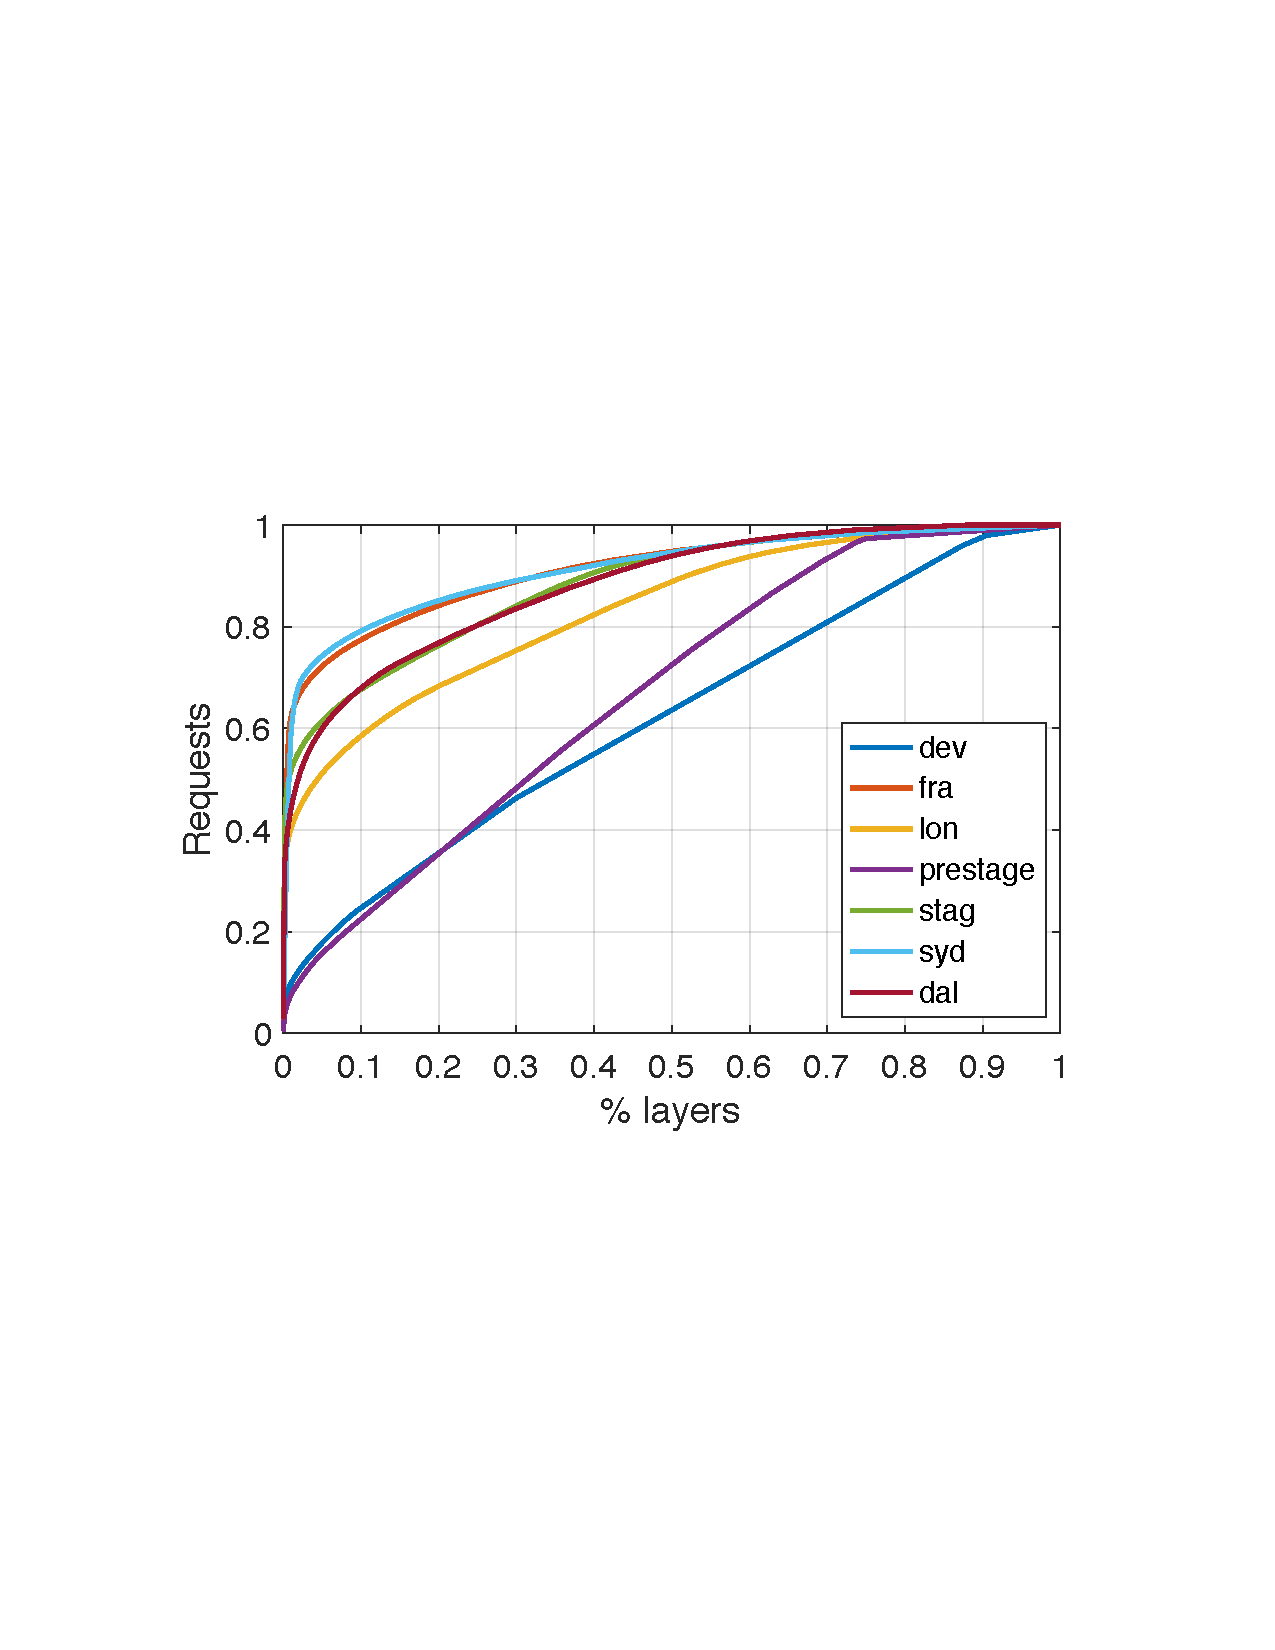
\includegraphics[width=1\textwidth]{graphs/layer_skewness.pdf}
%			%\caption{CDF of layer  count.}
%		%	\vspace{-3pt}
%			\label{fig:layer-skenwess}
%		\end{minipage}
%			\begin{minipage}{0.32\linewidth}
%				\centering
%				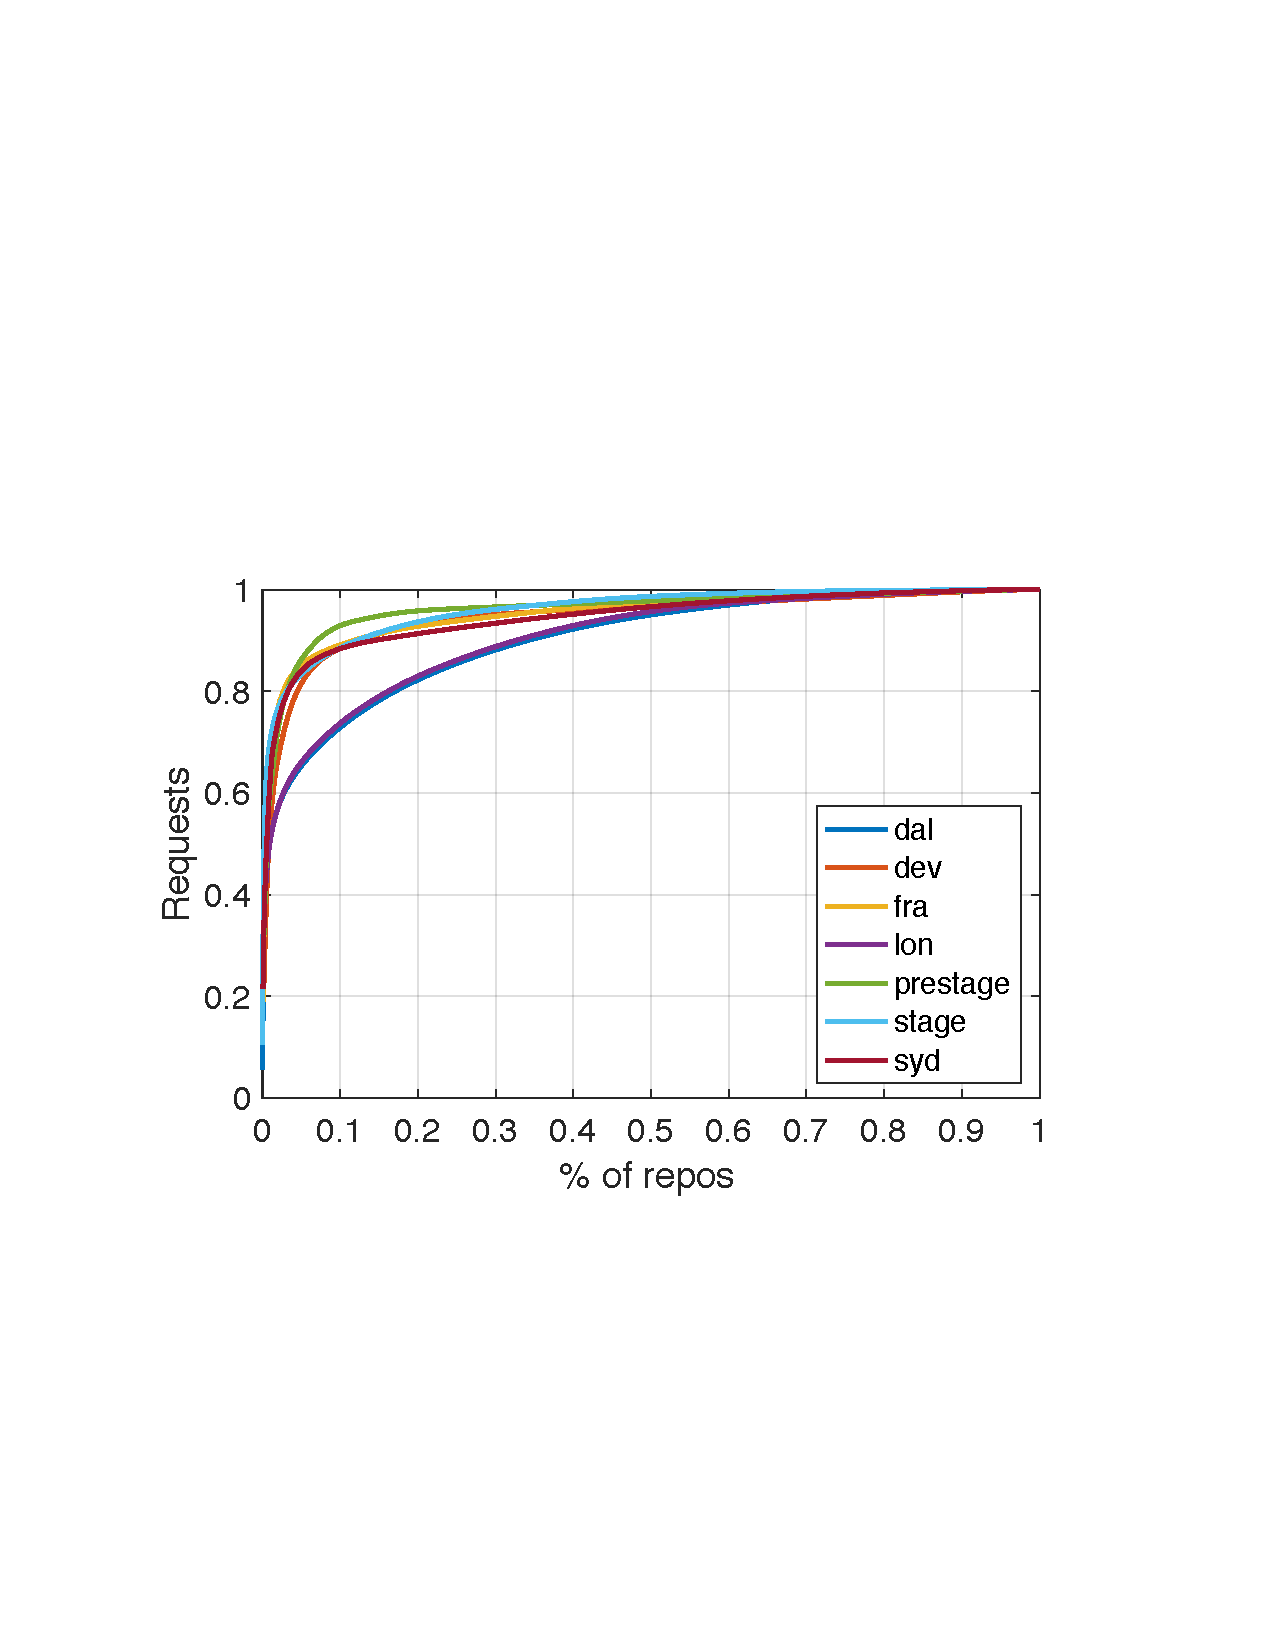
\includegraphics[width=1\textwidth]{graphs/repo-skewness.pdf}
%				%\caption{PDF of repository repulling probability.}
%				%	\vspace{-3pt}
%				\label{fig:repo-skewness}
%			\end{minipage}
%		\hfill
%		\begin{minipage}{0.32\linewidth}
%			\centering
%			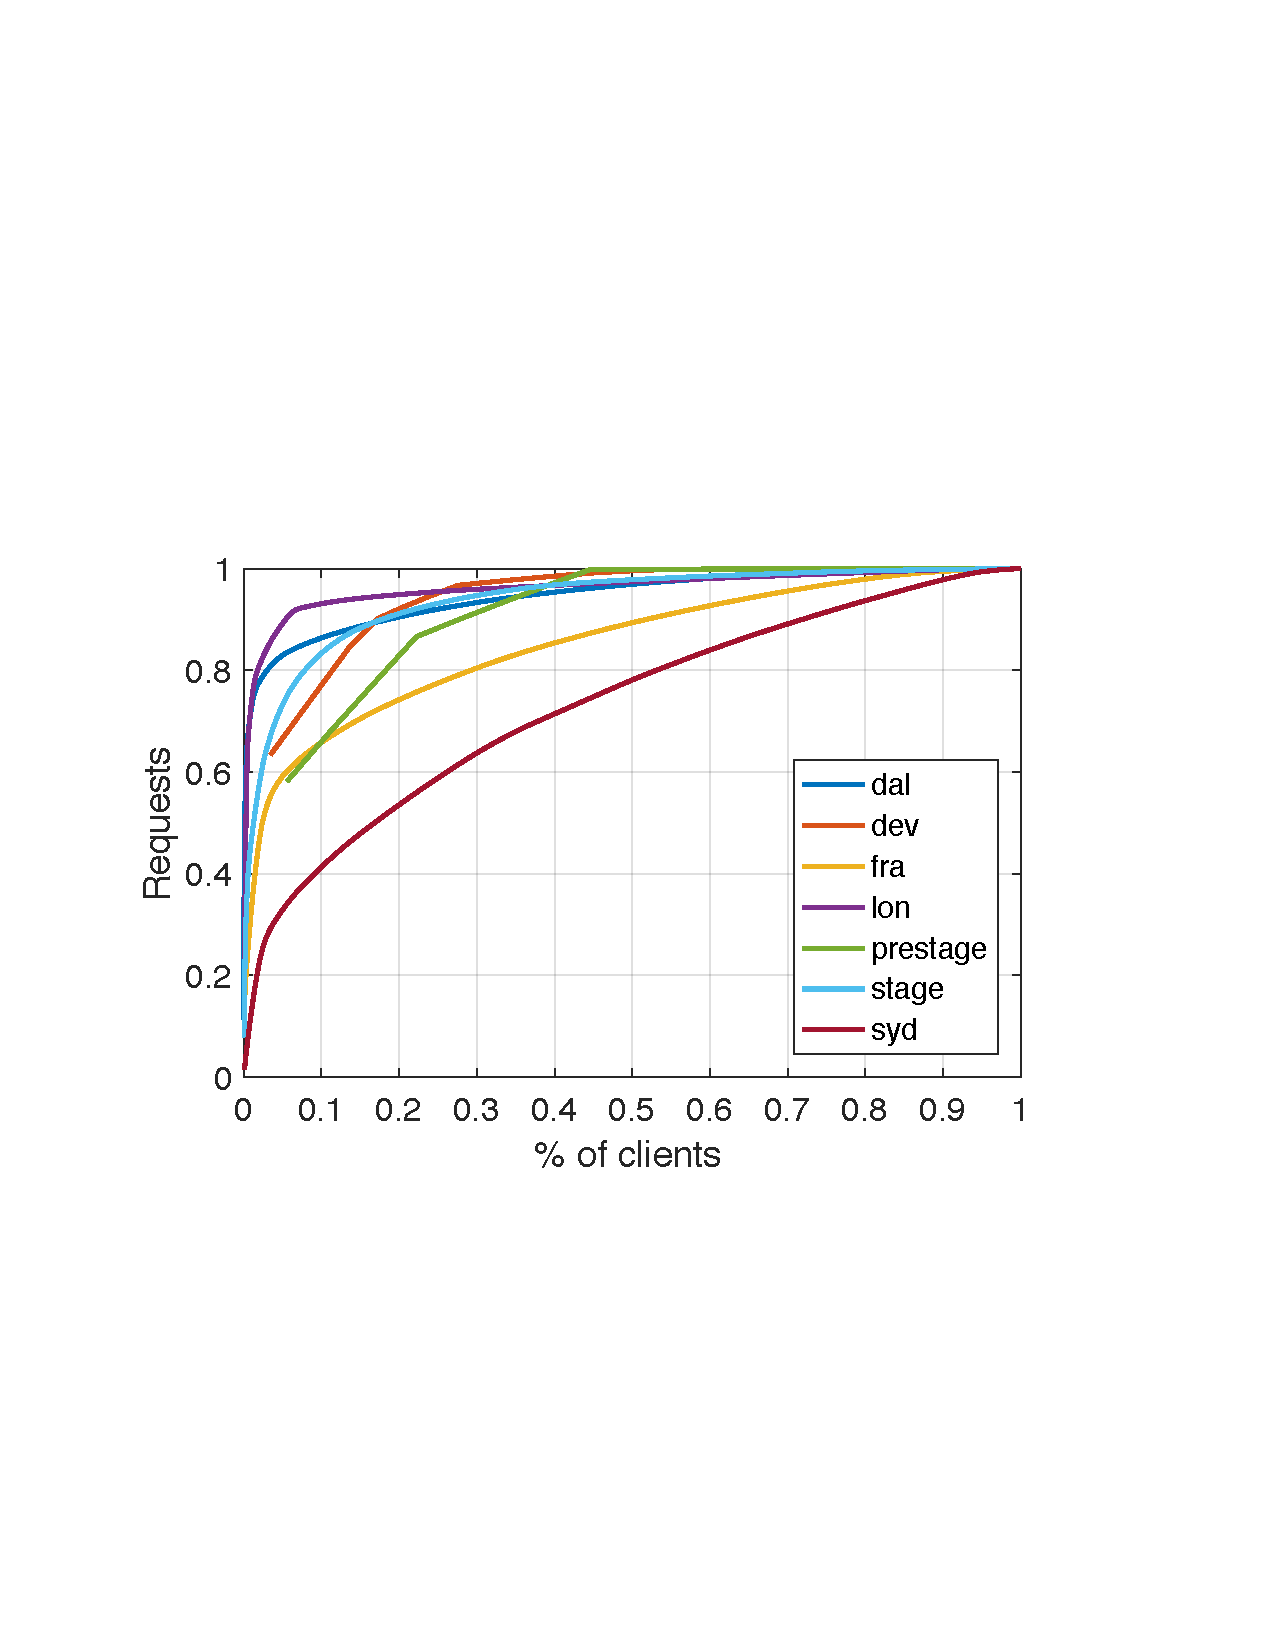
\includegraphics[width=1\textwidth]{graphs/client-skewness.pdf}
%			%\caption{PDF of client repulling probability.}
%			%	\vspace{-3pt}
%			\label{fig:client-skewness}
%			
%		\end{minipage}
%\caption{PDF of probability for layers, repositories, and clients.}
%%	\label{}
%\end{figure*}

\begin{figure*}[!t]
	\centering
	\subfigure[Layer repull count]{
		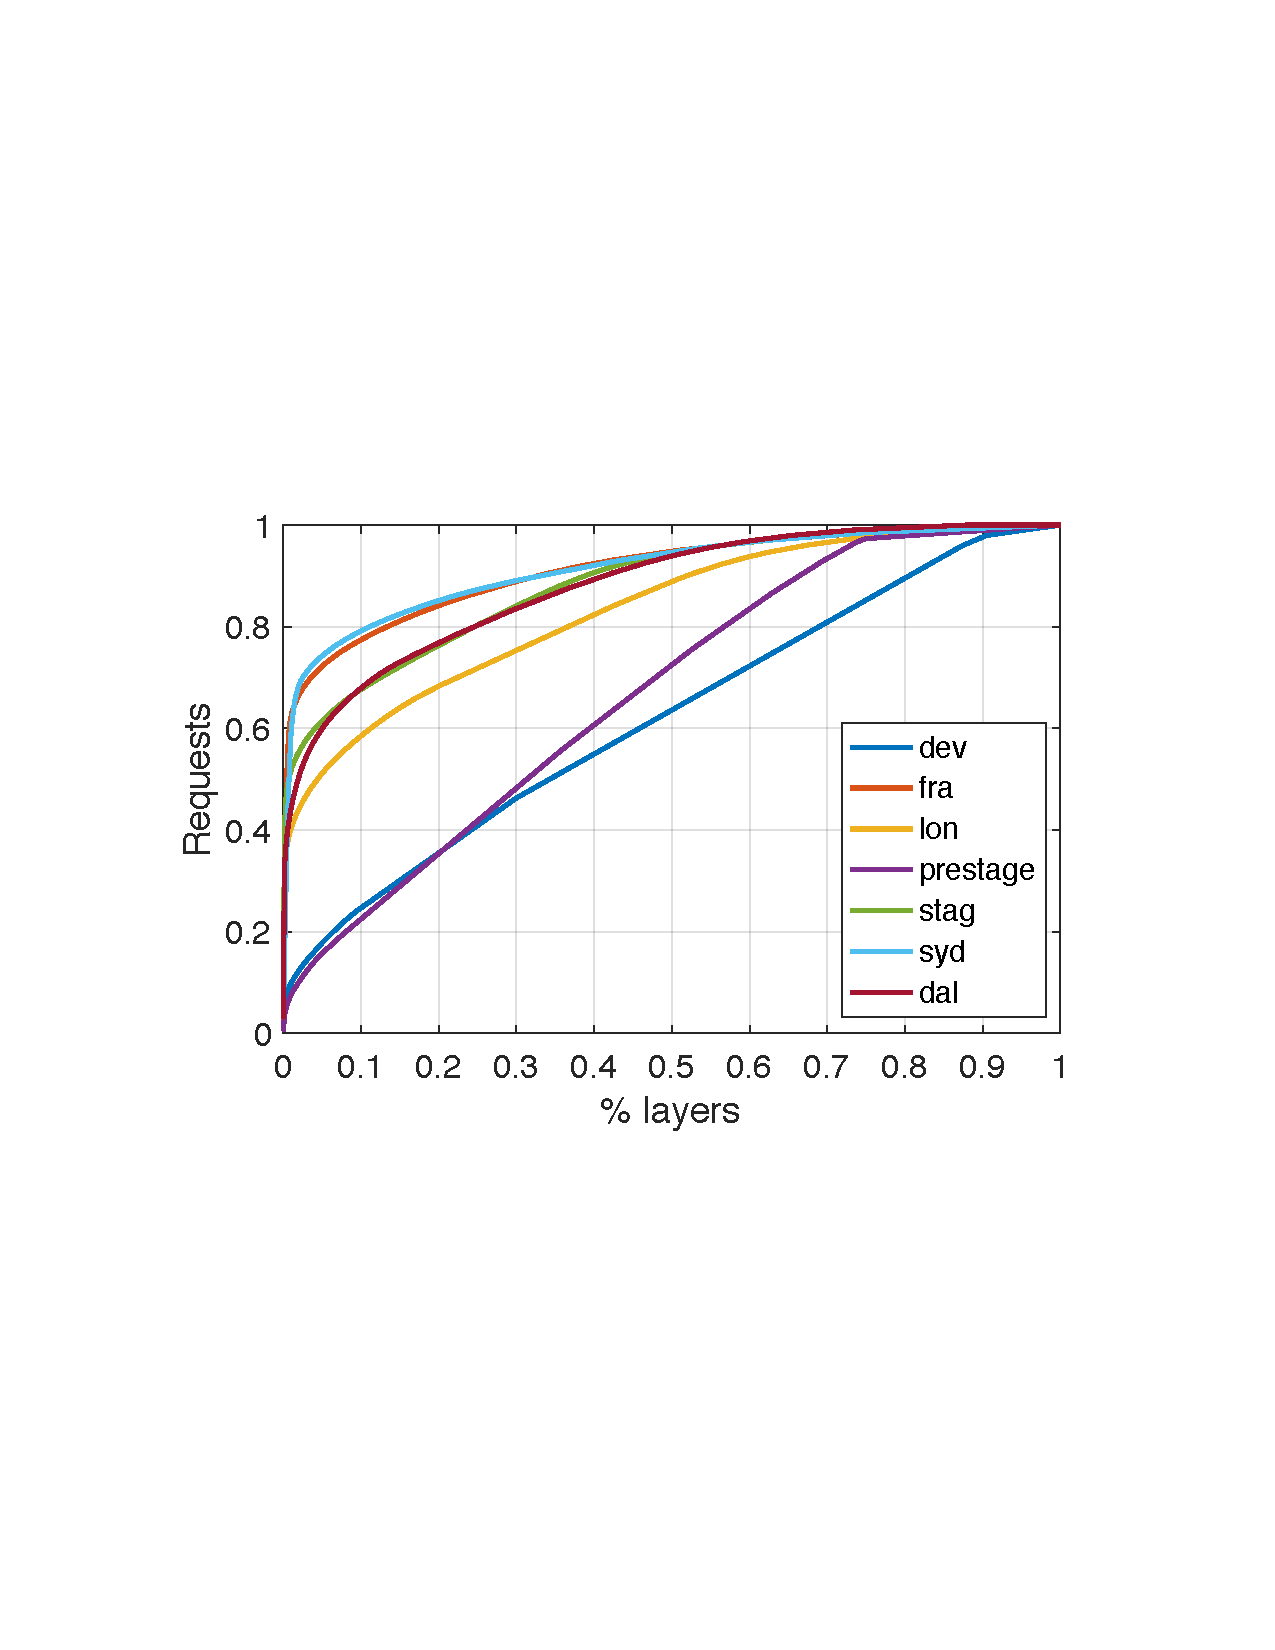
\includegraphics[width=0.2\linewidth]{graphs/layer_skewness.pdf}
		\label{fig:layer-skenwess}
	}
	\subfigure[Repository repulling probability]{
		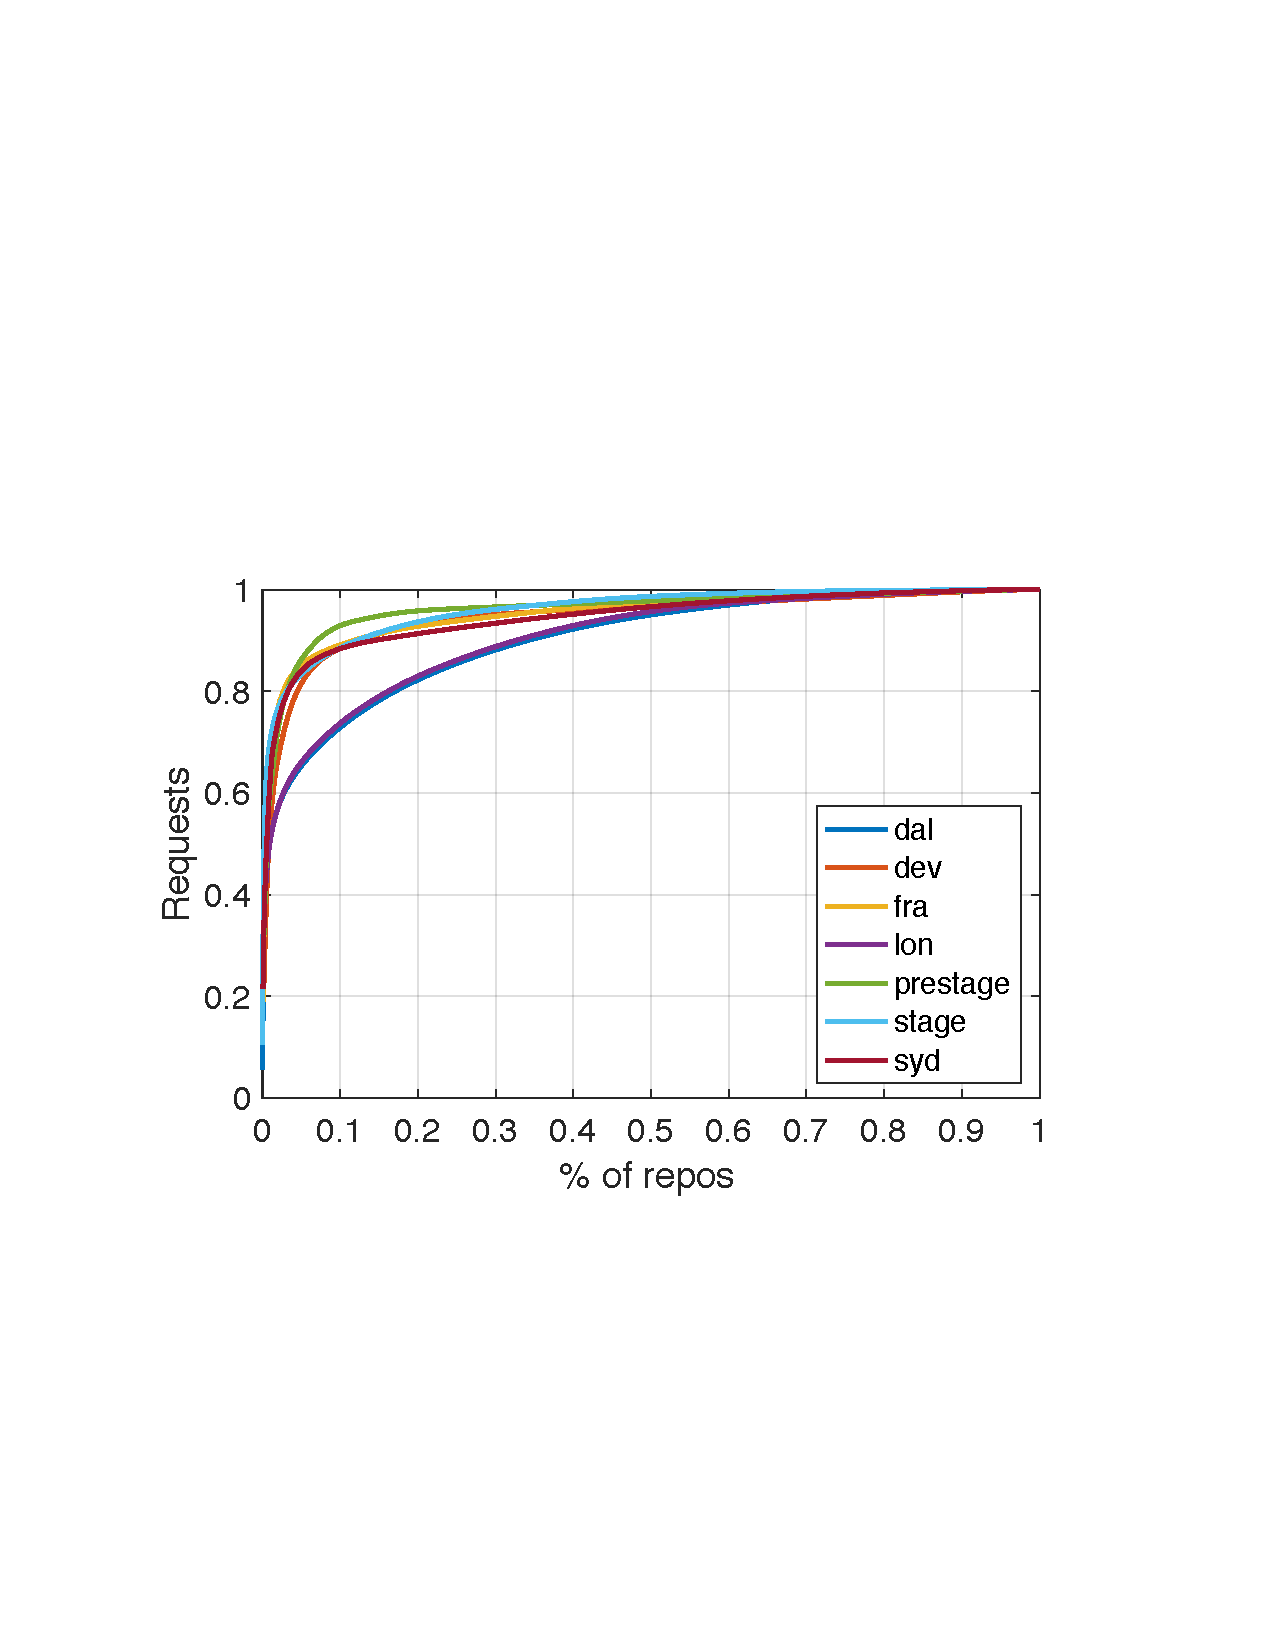
\includegraphics[width=0.2\linewidth]{graphs/repo-skewness.pdf}
		\label{fig:repo-skewness}
	}
	\subfigure[Client repulling probability]{
		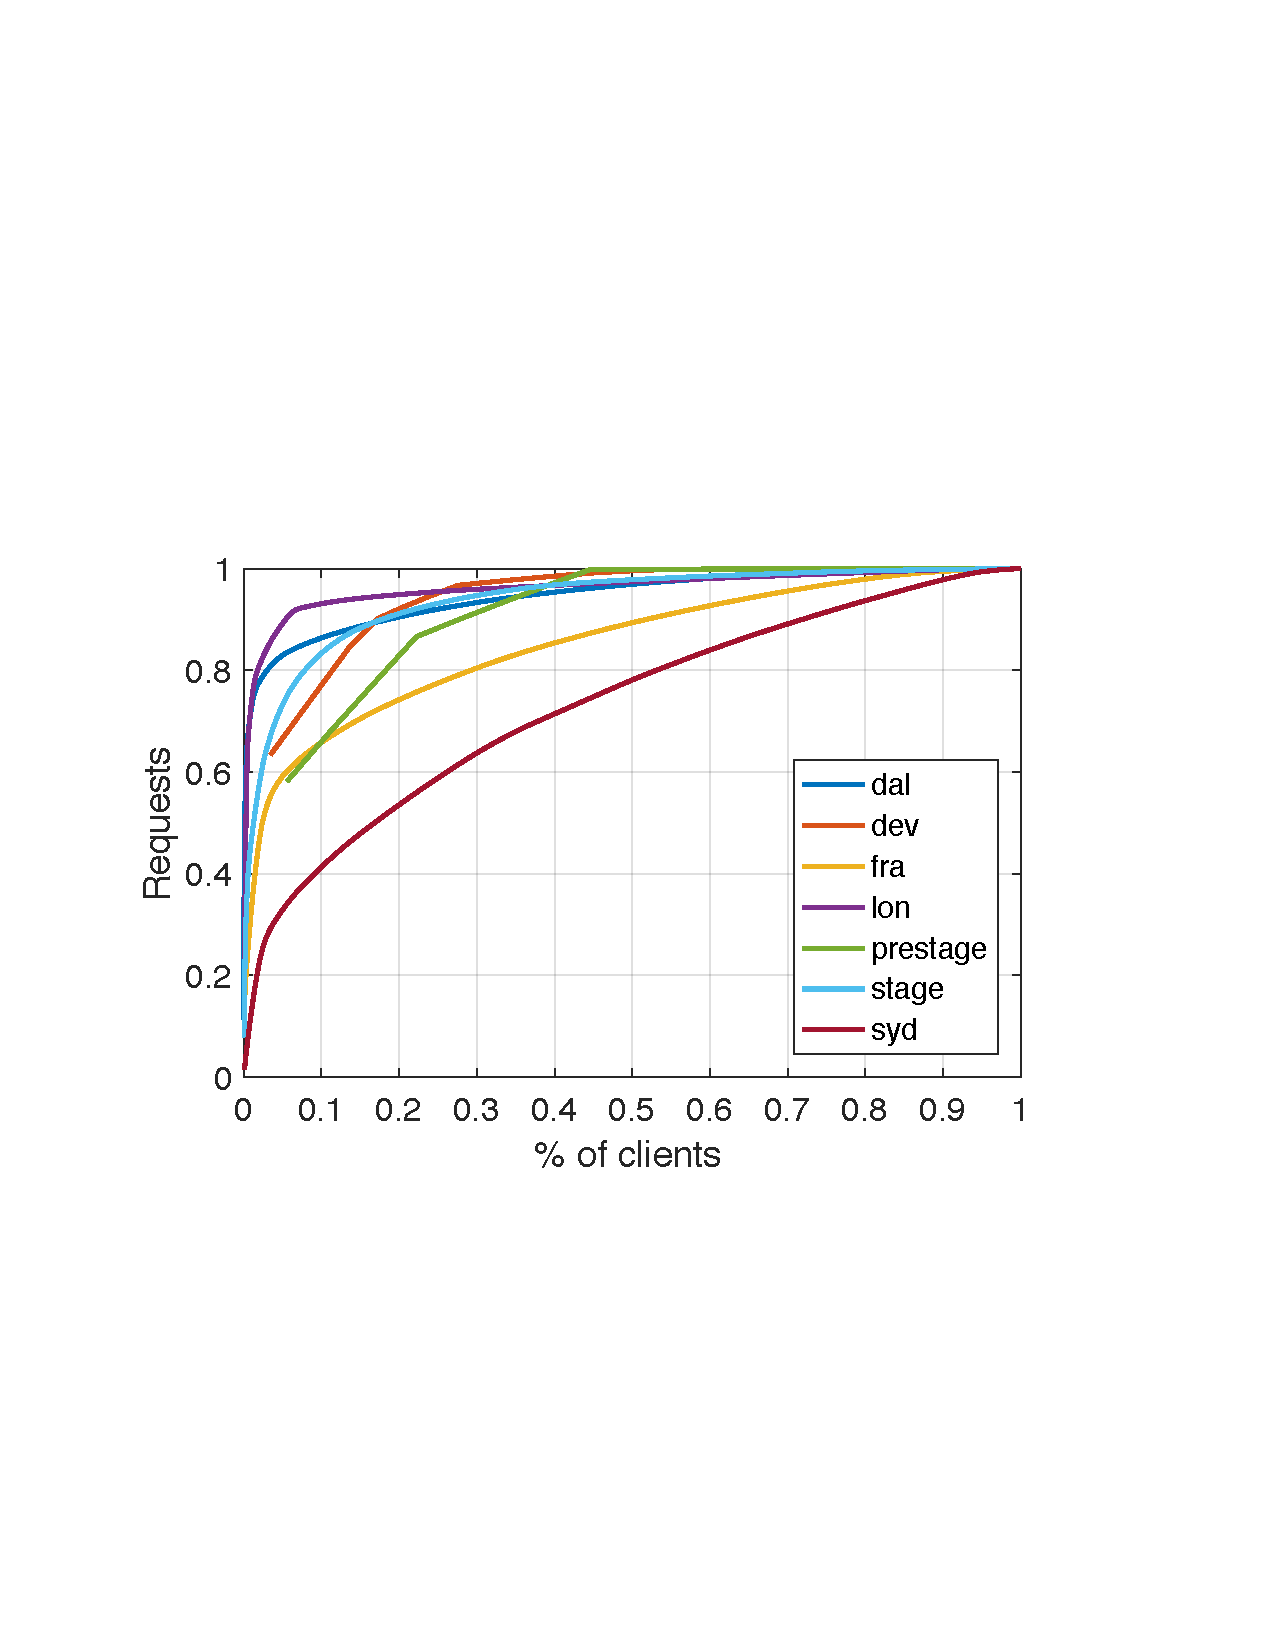
\includegraphics[width=0.2\linewidth]{graphs/client-skewness.pdf}
 	\label{fig:client-skewness}
	}
\caption{PDF of probability for layers, repositories, and clients.}
	\label{fig-skewness}
\end{figure*}
%=======
%\paragraph{User access patterns.} 
%
%\paragraph{Pull once VS. Always pull.}
%\HA{I think we should start the paragraph by stating that we are profiling users based on their behavior in repulling a repository and why}
%Figure~\ref{fig:layer-repull-cdf} shows the CDF of layer repull count. Here, \emph{repulling} indicates the act of pulling a layer that was previously pulled by the user because it is no longer present on the user's side.
%The majority of repulled layers are infrequently repulled.
%$83$\% of the repulled layers are only repulled twice.
%For example, only $3$\% of the layers from \texttt{Syd} are repulled more than twice.
%
%When different clients \texttt{pull} the same repository, 
%each client will only fetch, from the repository, the layers that are not present in their local layer dataset. Layers present locally on each client side vary with time as clients clear layer data. This makes clients pull different layers at different times.
%%they will fetch different amount of layers from the repository based on the contents of their local layer dataset. The local layers can vary with time due to clearing of the data so the same clients can fetch different amounts of layers at different times.
%Hence, a \texttt{pull manifest} request doesn't usually result in repulling all the layers in the repository. 
%Here, we define \emph{repulling a repository} as repulling the layers in the repository by the same client.
%Figure~\ref{fig:repo-repull-cdf} shows the CDF of the probability of repulling a repository, calculated by dividing the number of \texttt{pull manifest} requests resulting in repository repulls, by 
%the total number of \texttt{pull manifest} requests issued for the same repository.
%We see that the majority of repositories are not repulled.
%The percentage of repositories whose repull probability is zero (\ie are pulled only once by a client) ranges from $57$\% for \texttt{Prestage} to $85$\% for \texttt{Syd}.
%Only $20$\% of repositories from  \texttt{Prestage}, \texttt{Stage}, and 
%\texttt{Syd} have a repulling probability higher than $0.5$.
%We also observe that few repositories' repulling probability is $1$, indicating repulls everytime by the clients.
%
%Figure~\ref{fig:client-repull-cdf} shows the client repulling probability, calculated by dividing the number of \emph{repull} layer requests from a client, by
%the total number of \texttt{pull} layer requests issued by the same client.
%$60$\% of clients from \texttt{Prestage}, \texttt{Dev}, \texttt{Lon}, and \texttt{Fra} have a repulling probability lower than $0.1$.
%$2$\%-$12$\% of clients have a repulling probability higher than $0.9$ from workloads:
%\texttt{Dal}, \texttt{Dev}, \texttt{Fra}, \texttt{Prestage},
%\texttt{Stage}, \texttt{Syd}, and \texttt{Lon}.
%
%From the probability distribution of the clients repulling, we can observe that a significant chunk of the clients %are rarely repulling a repository
% have a very low repulling probability and another chunk of the clients have a very high repulling probability, with few clients in the middle. For simplicity of implementation, the high probability clients can be classified as always repulling clients, and the low probability clients as never repulling (i.e. they pull only once). The few clients in the middle are considered erratic  and no classification is made for them.
%
%
%
%\subsection{Temporal Access Patterns}
%%\begin{figure*}[t]
%		\begin{minipage}{0.32\linewidth}
%			\centering
%			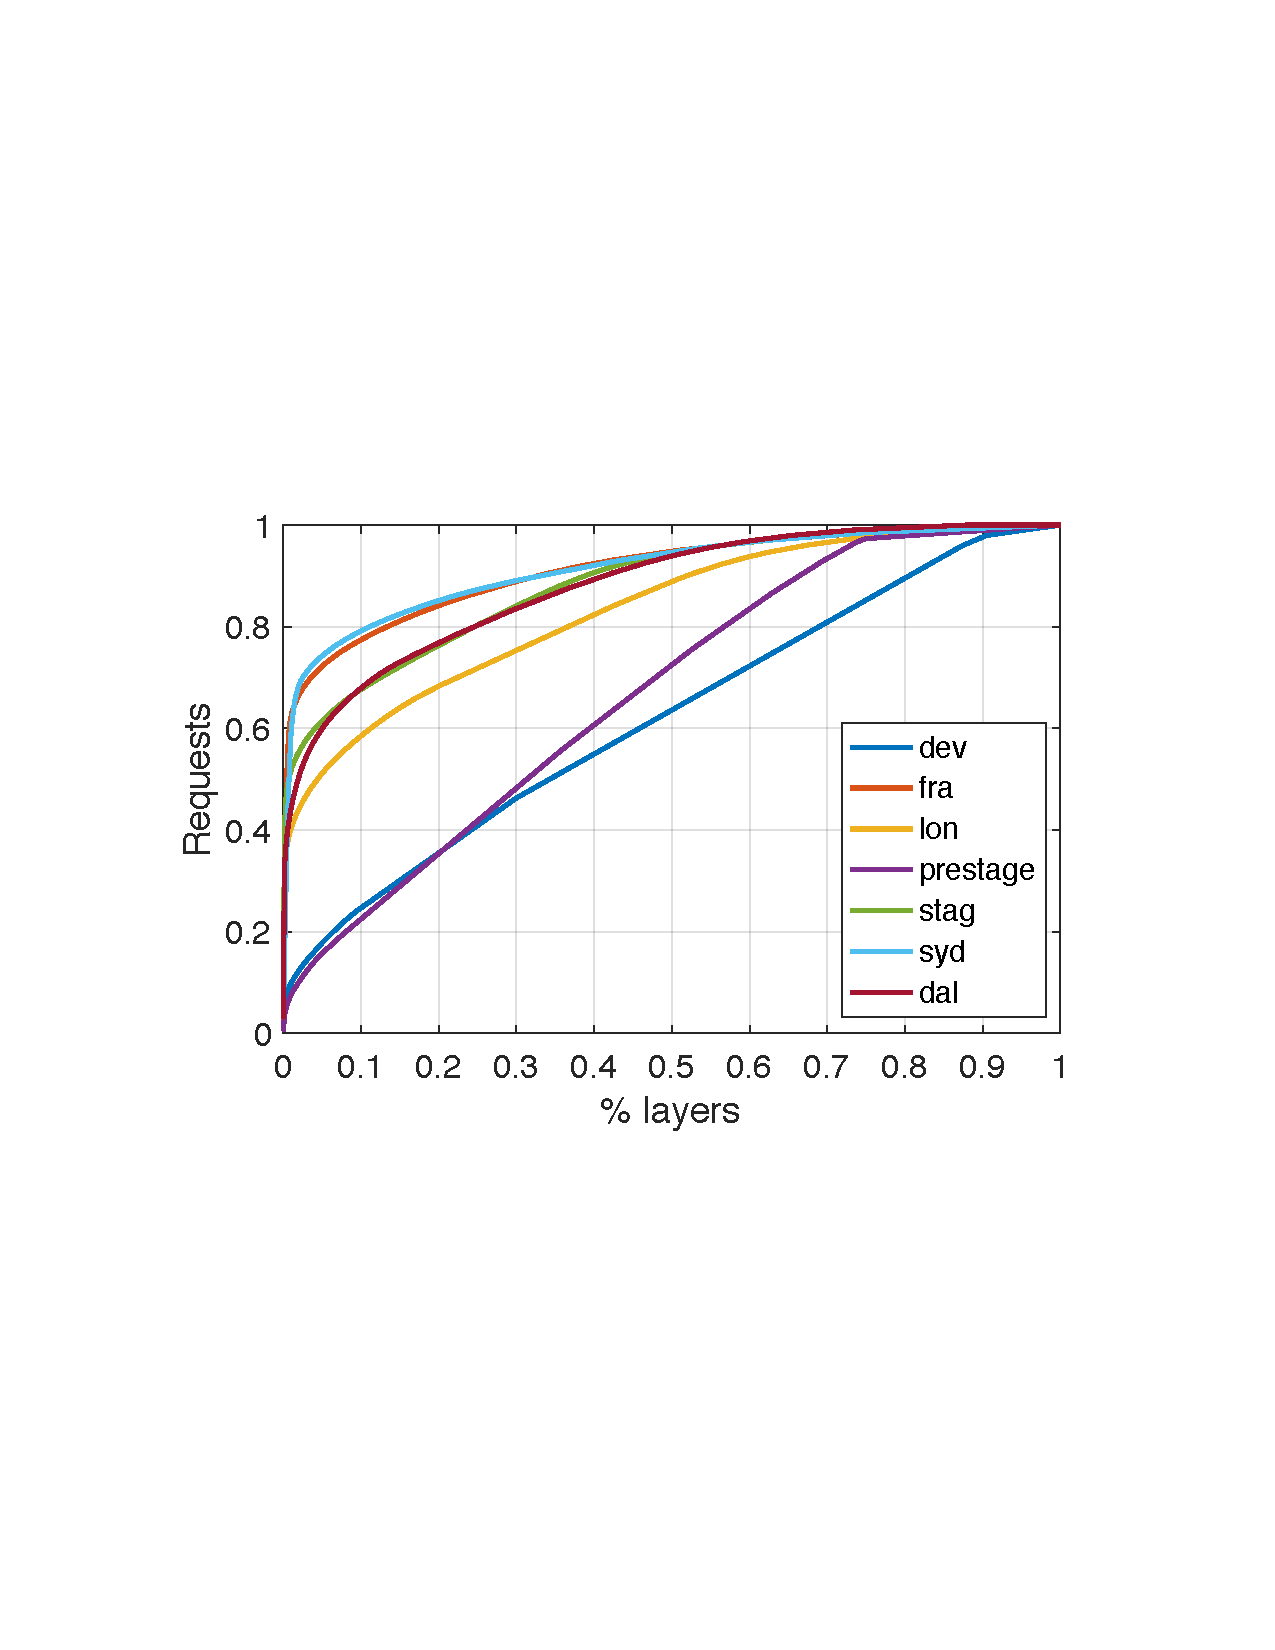
\includegraphics[width=1\textwidth]{graphs/layer_skewness.pdf}
%			%\caption{CDF of layer  count.}
%		%	\vspace{-3pt}
%			\label{fig:layer-skenwess}
%		\end{minipage}
%			\begin{minipage}{0.32\linewidth}
%				\centering
%				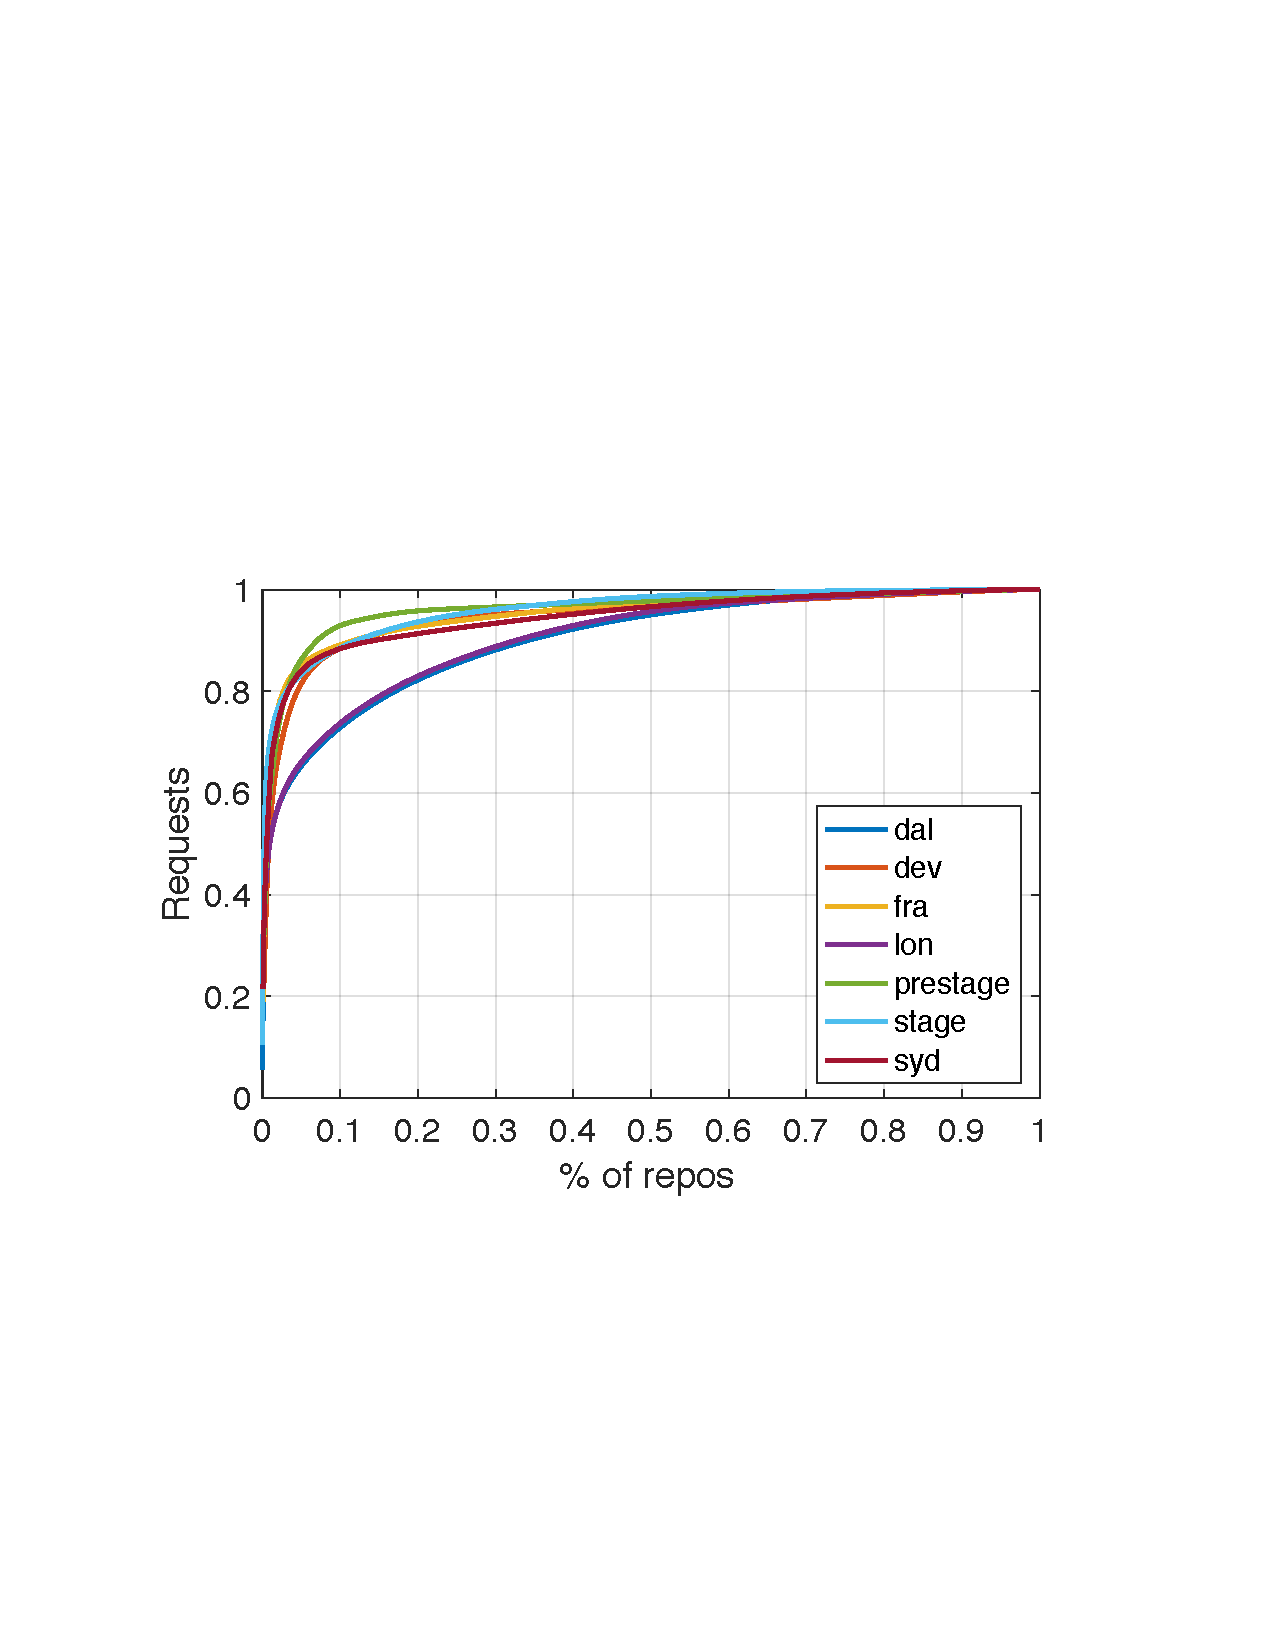
\includegraphics[width=1\textwidth]{graphs/repo-skewness.pdf}
%				%\caption{PDF of repository repulling probability.}
%				%	\vspace{-3pt}
%				\label{fig:repo-skewness}
%			\end{minipage}
%		\hfill
%		\begin{minipage}{0.32\linewidth}
%			\centering
%			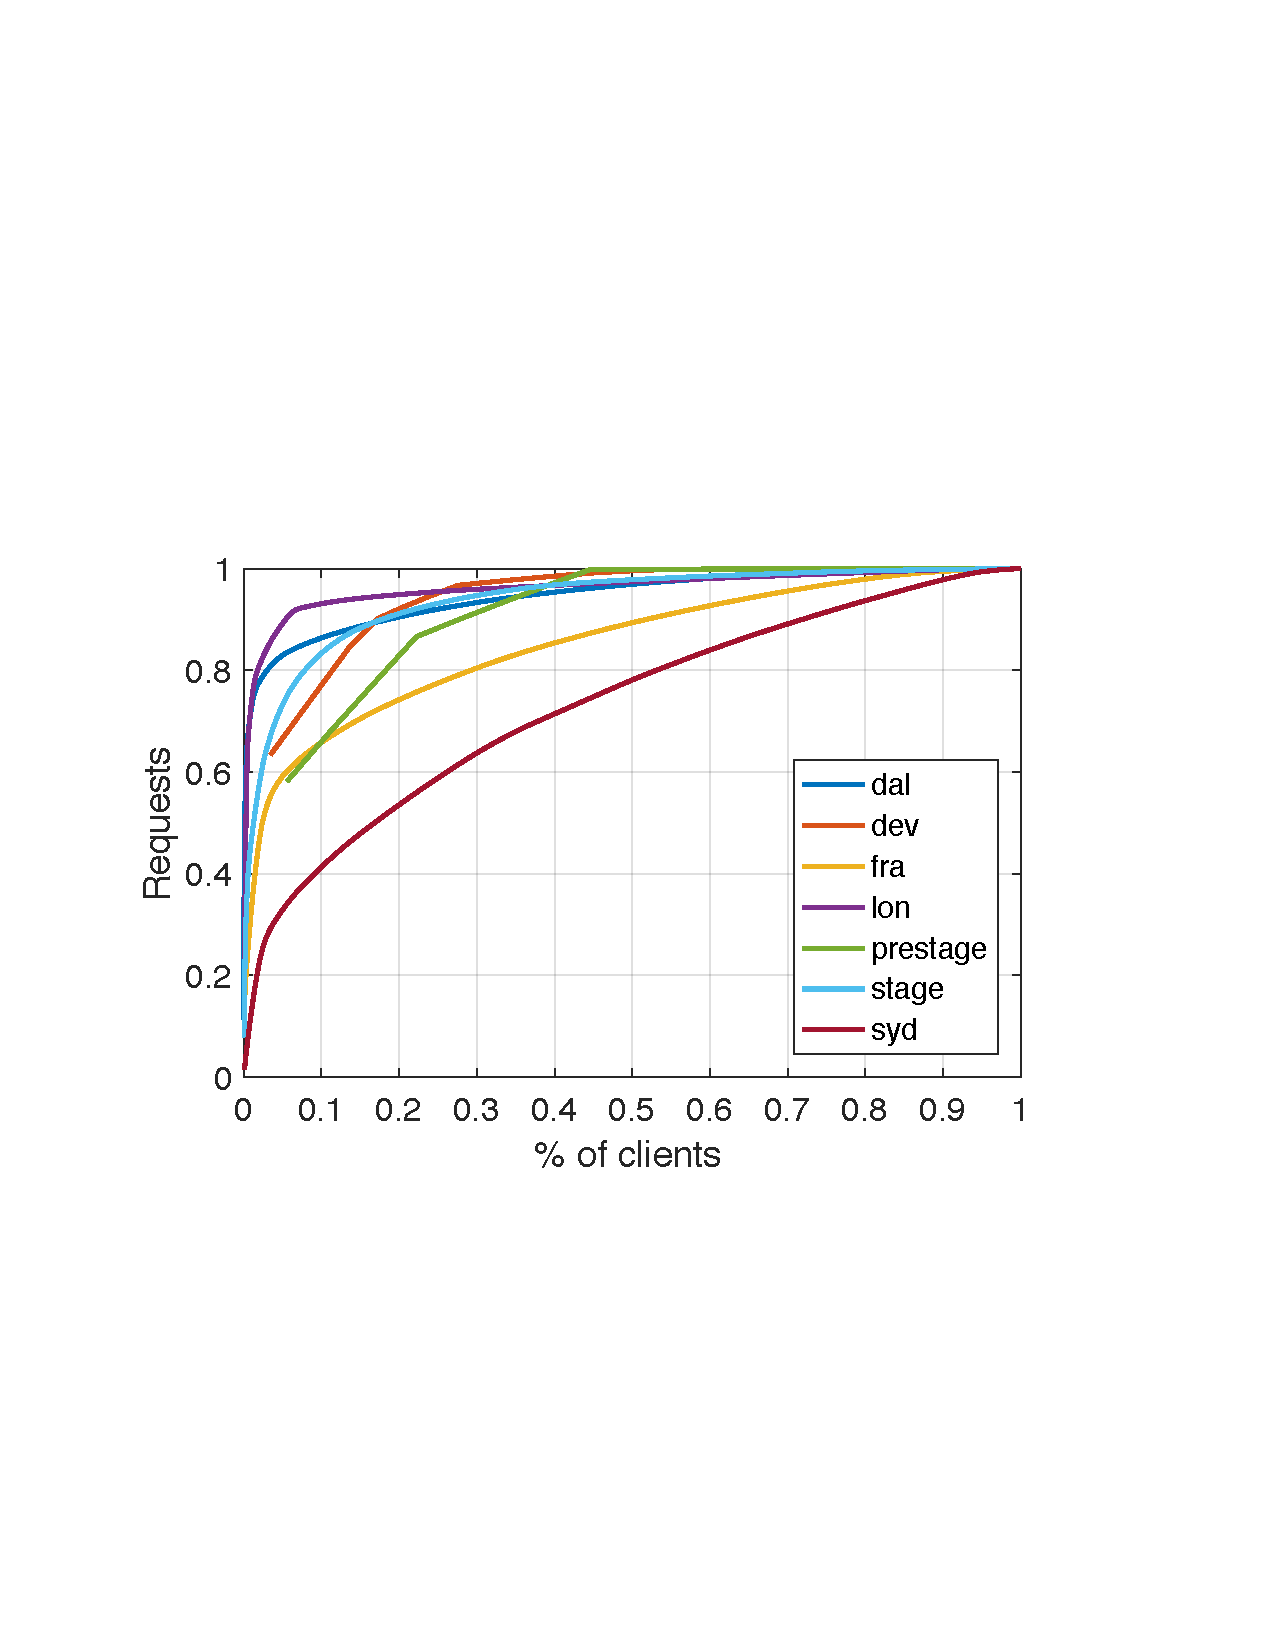
\includegraphics[width=1\textwidth]{graphs/client-skewness.pdf}
%			%\caption{PDF of client repulling probability.}
%			%	\vspace{-3pt}
%			\label{fig:client-skewness}
%			
%		\end{minipage}
%\caption{PDF of probability for layers, repositories, and clients.}
%%	\label{}
%\end{figure*}

\begin{figure*}[!t]
	\centering
	\subfigure[Layer repull count]{
		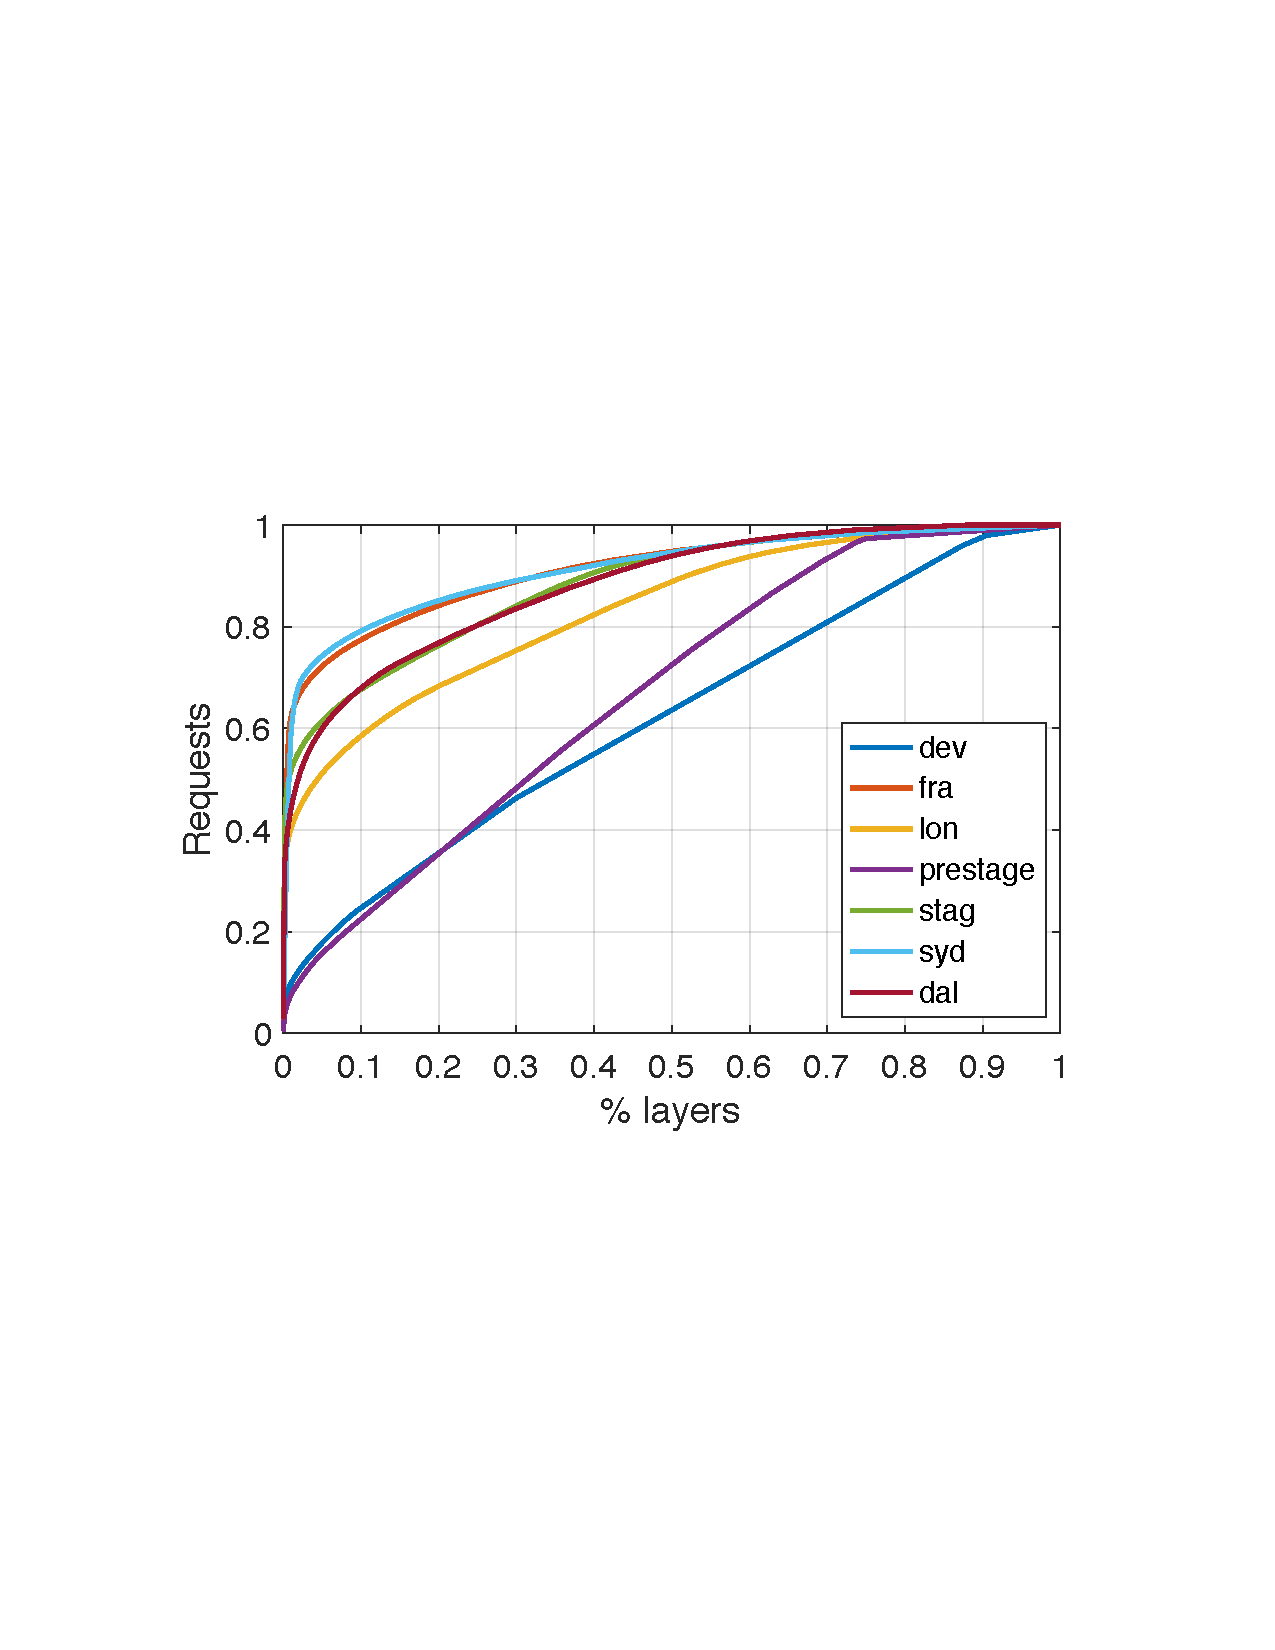
\includegraphics[width=0.2\linewidth]{graphs/layer_skewness.pdf}
		\label{fig:layer-skenwess}
	}
	\subfigure[Repository repulling probability]{
		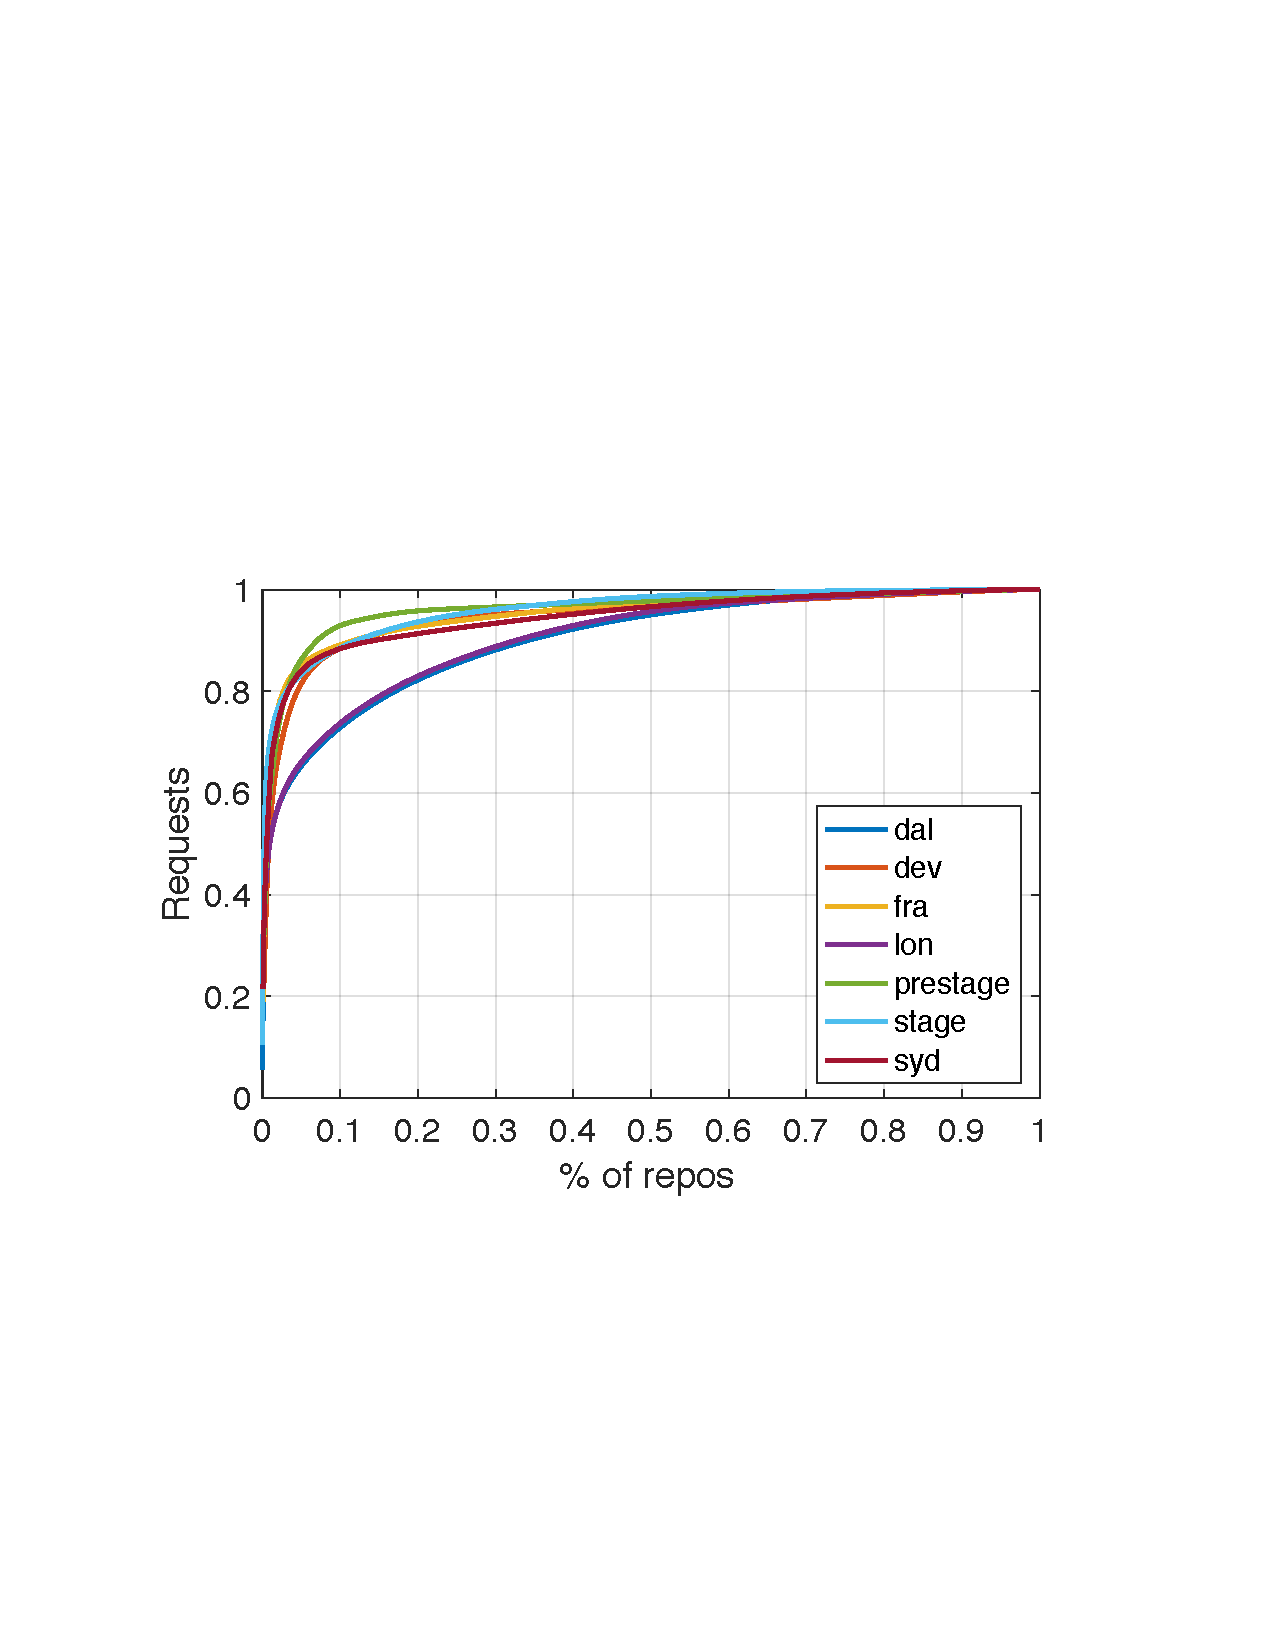
\includegraphics[width=0.2\linewidth]{graphs/repo-skewness.pdf}
		\label{fig:repo-skewness}
	}
	\subfigure[Client repulling probability]{
		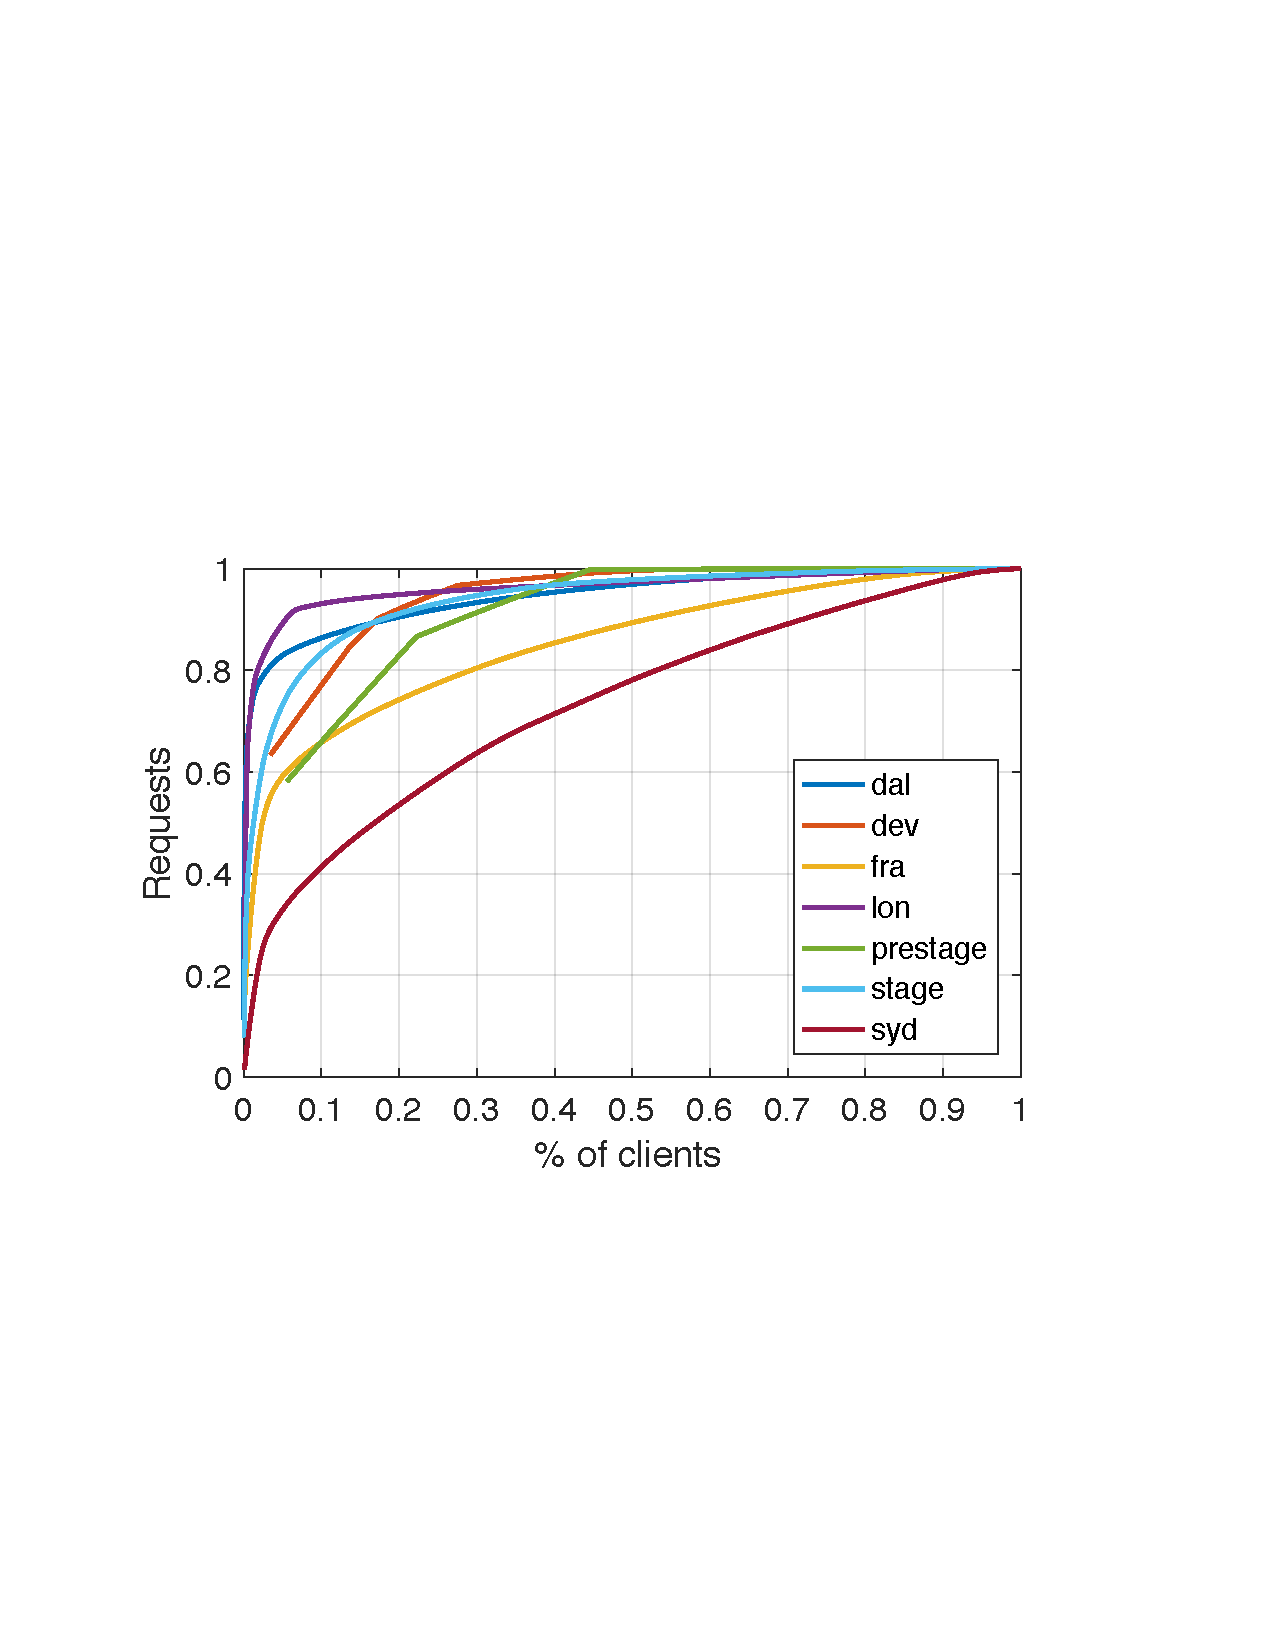
\includegraphics[width=0.2\linewidth]{graphs/client-skewness.pdf}
 	\label{fig:client-skewness}
	}
\caption{PDF of probability for layers, repositories, and clients.}
	\label{fig-skewness}
\end{figure*}
%>>>>>>> 94daa3df1d5d977ac11fd9da2aea7b4eed340be2
%\begin{figure*}[t]
%		\begin{minipage}{0.32\linewidth}
%			\centering
%			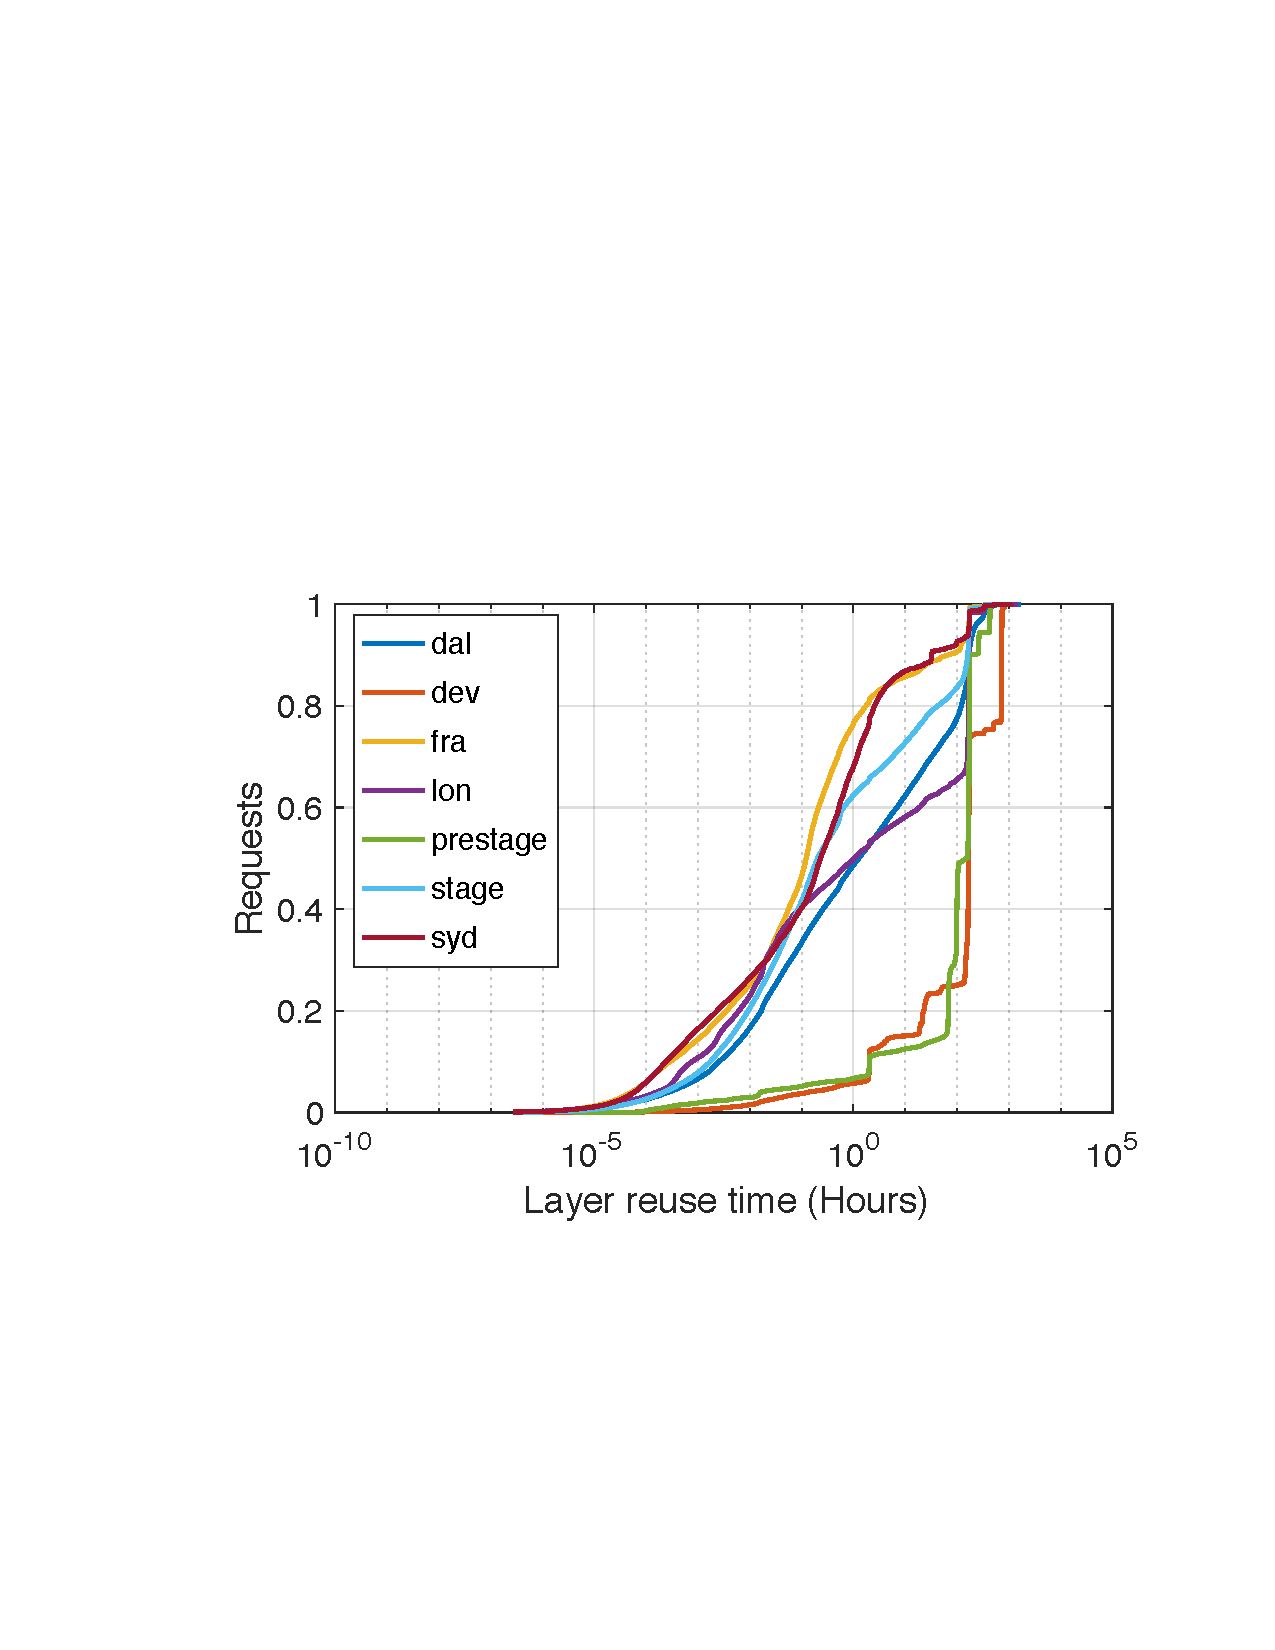
\includegraphics[width=1\textwidth]{graphs/layer-reusetime.pdf}
%		%	\caption{CDF of layer reuse time.}
%		%	\vspace{-3pt}
%			\label{fig:layer-reuse}
%		\end{minipage}
%			\begin{minipage}{0.32\linewidth}
%				\centering
%				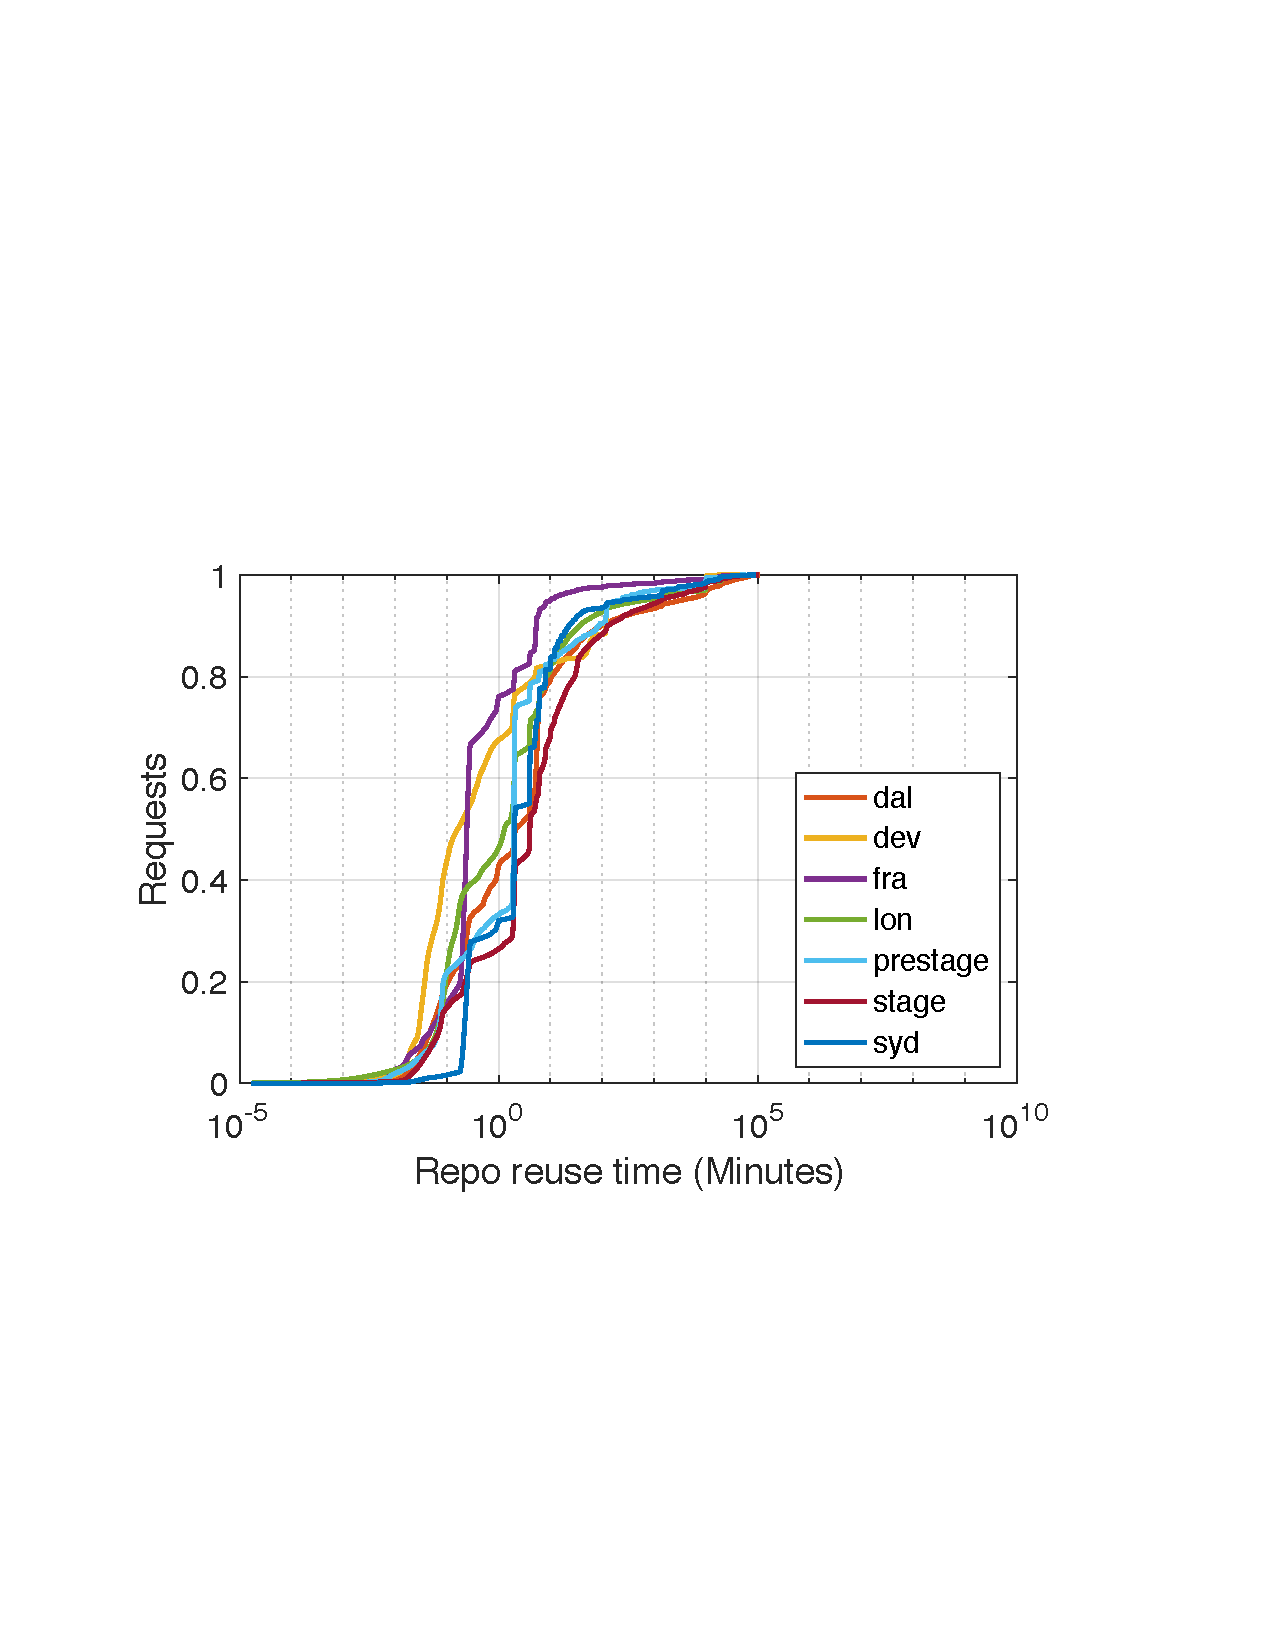
\includegraphics[width=1\textwidth]{graphs/repo-reusetime.pdf}
%			%	\caption{PDF of repository reuse time.}
%				%	\vspace{-3pt}
%				\label{fig:repo-reuse}
%			\end{minipage}
%		\begin{minipage}{0.32\linewidth}
%			\centering
%			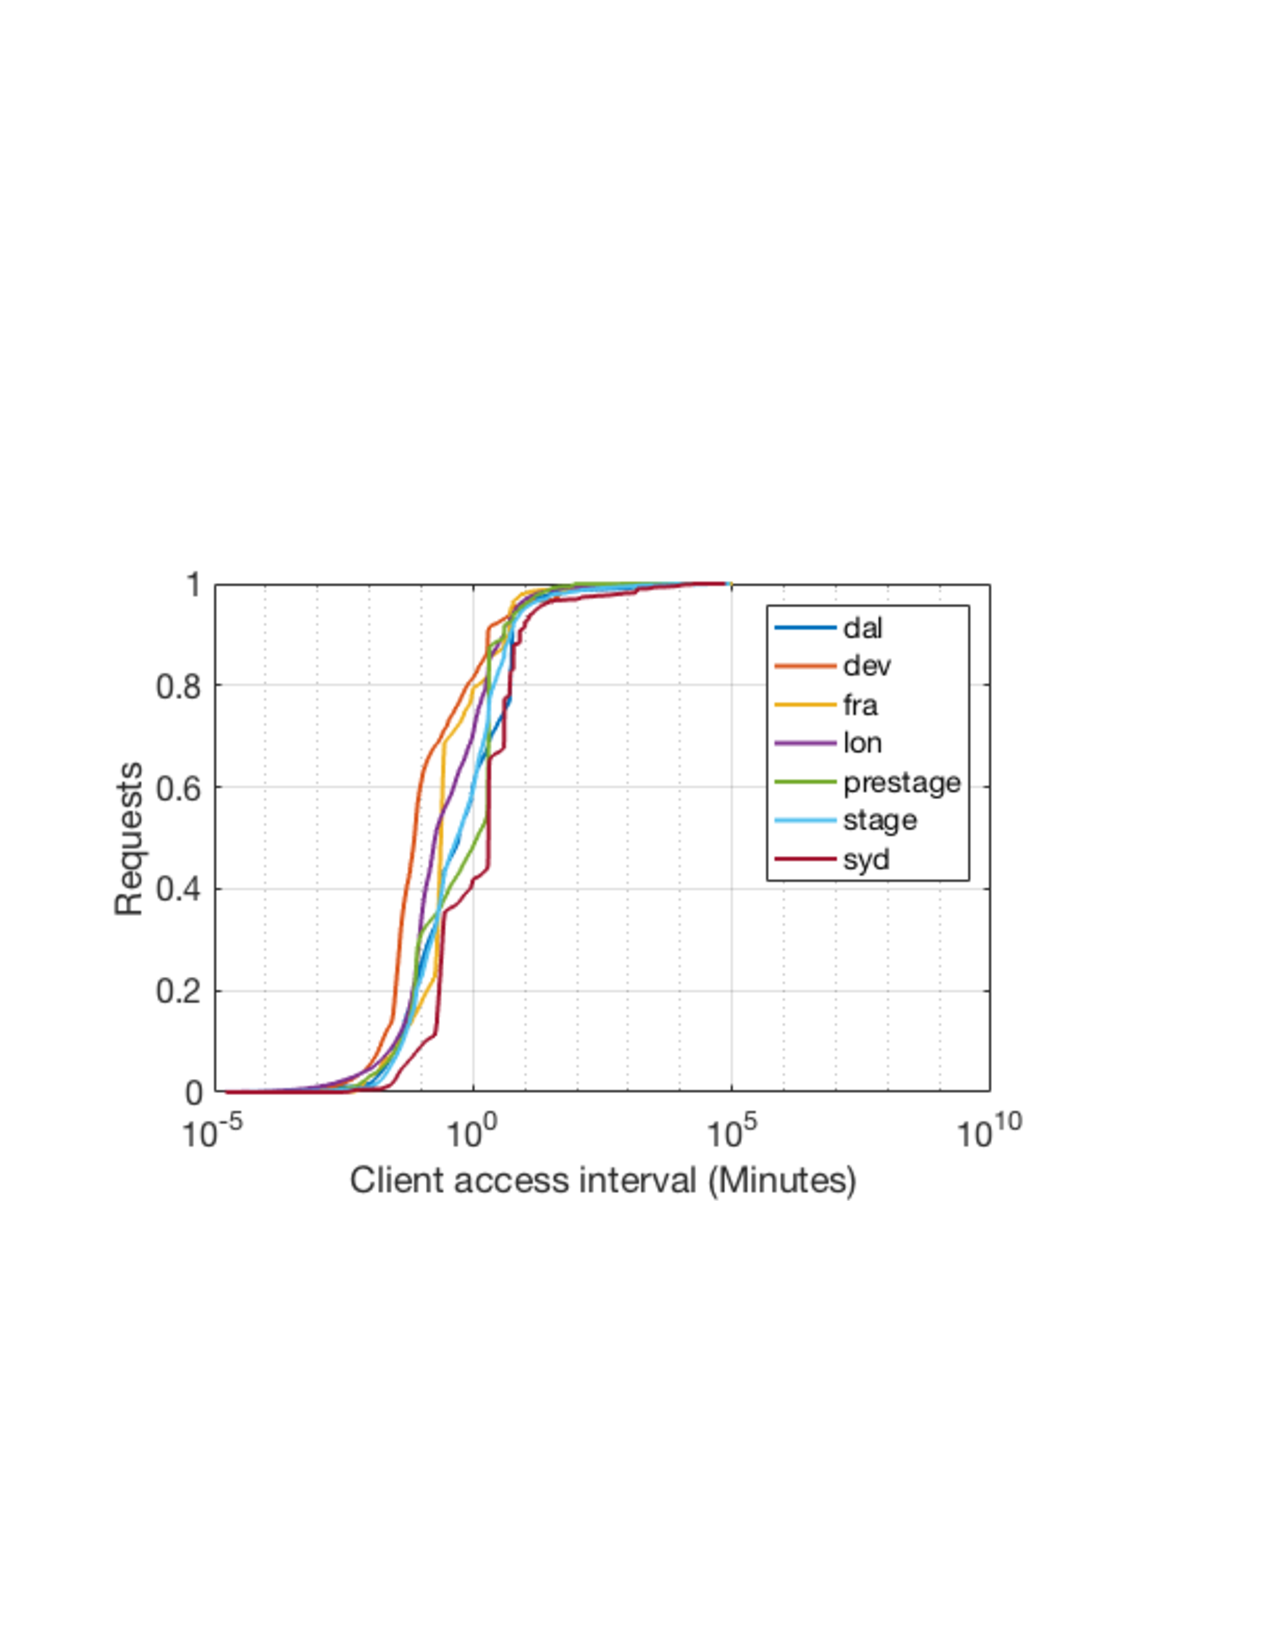
\includegraphics[width=1\textwidth]{graphs/user-intervals.pdf}
%			%\caption{PDF of client access intervals.}
%			%	\vspace{-3pt}
%			\label{fig:user-interval}
%		\end{minipage}
%	\caption{CDF of reusetime for layers, repositories and clients' access intervals.}
%	\label{fig:layer-reuse}
%\end{figure*}
\begin{figure}[t]
	\centering
	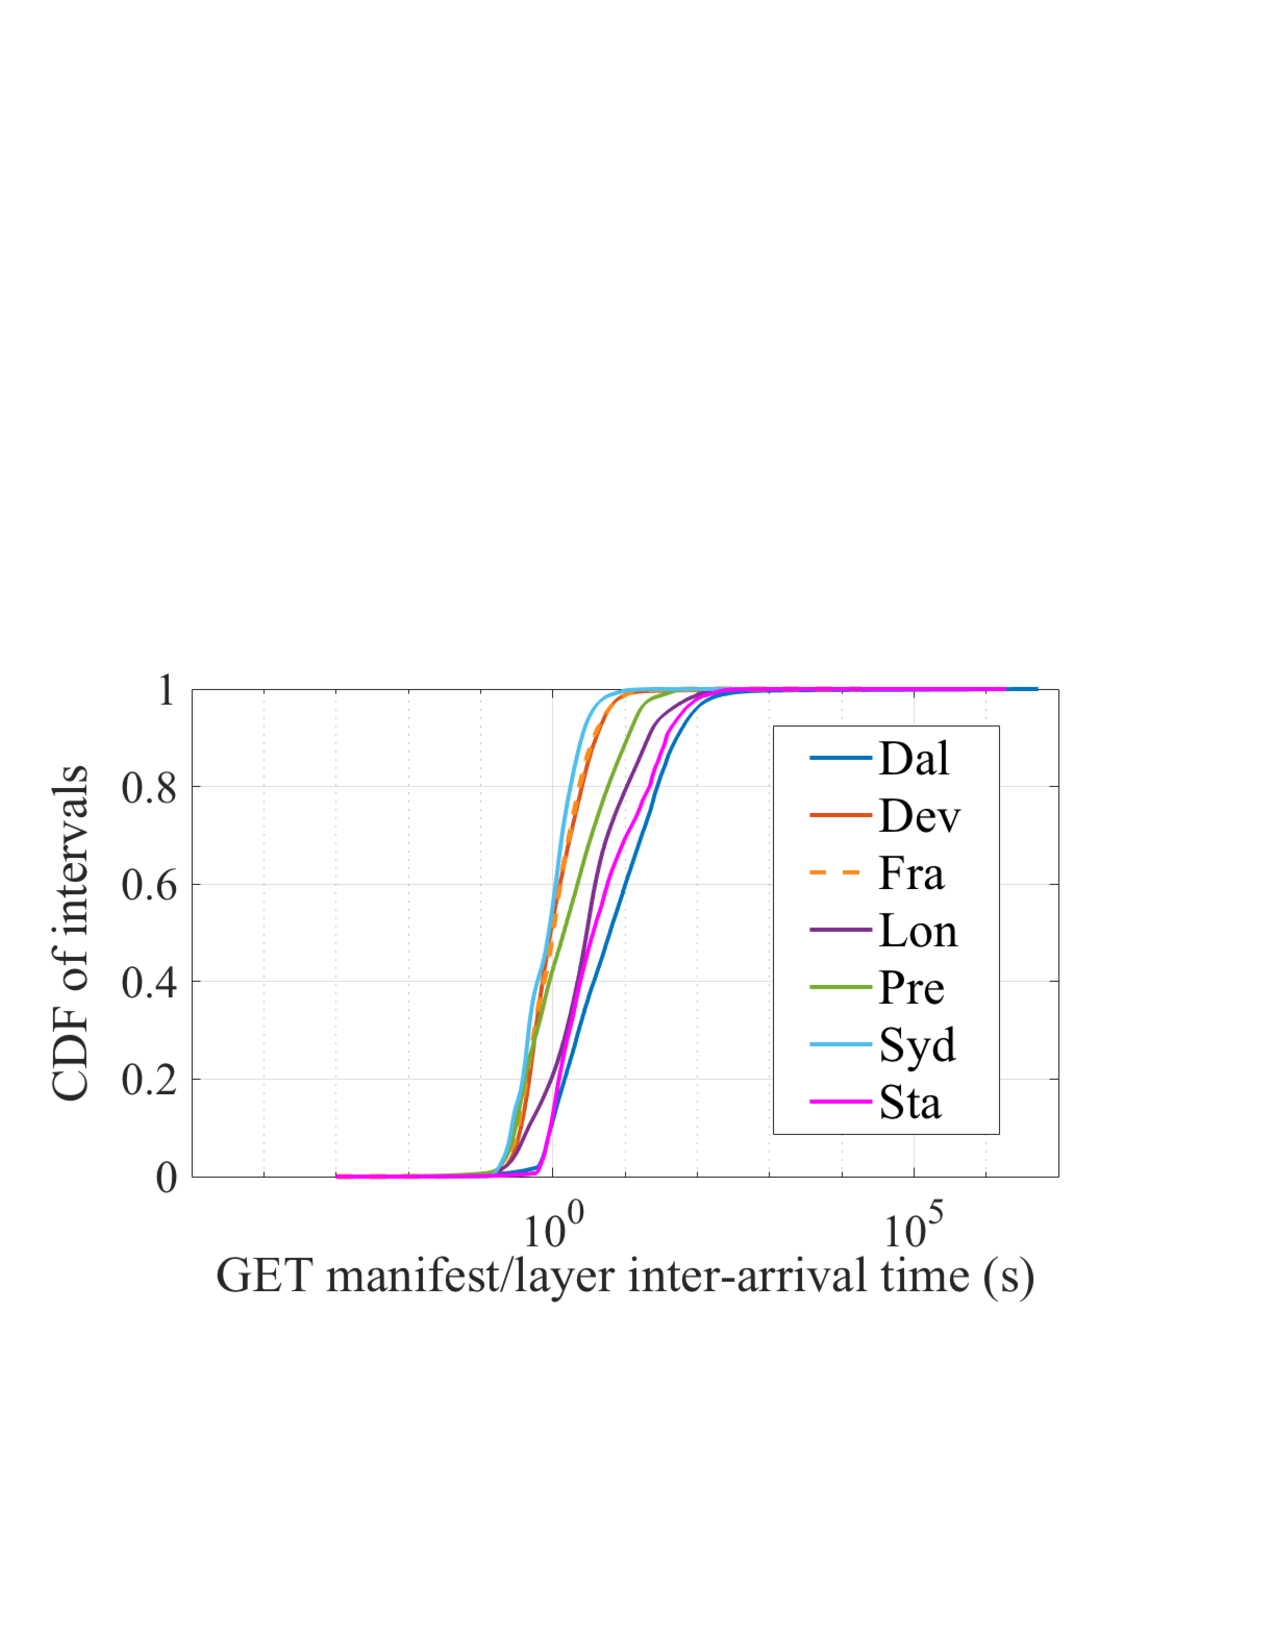
\includegraphics[width=0.3\textwidth]{graphs/GML-intervals.pdf}
	\caption{Intervals between \texttt{pull} manifest request and \texttt{pull} layer request}
	%	\vspace{-3pt}
	\label{fig:intervals}
	
\end{figure}
%\begin{figure*}[!t]
%	\centering
%	\subfigure[Layer repull count]{
%		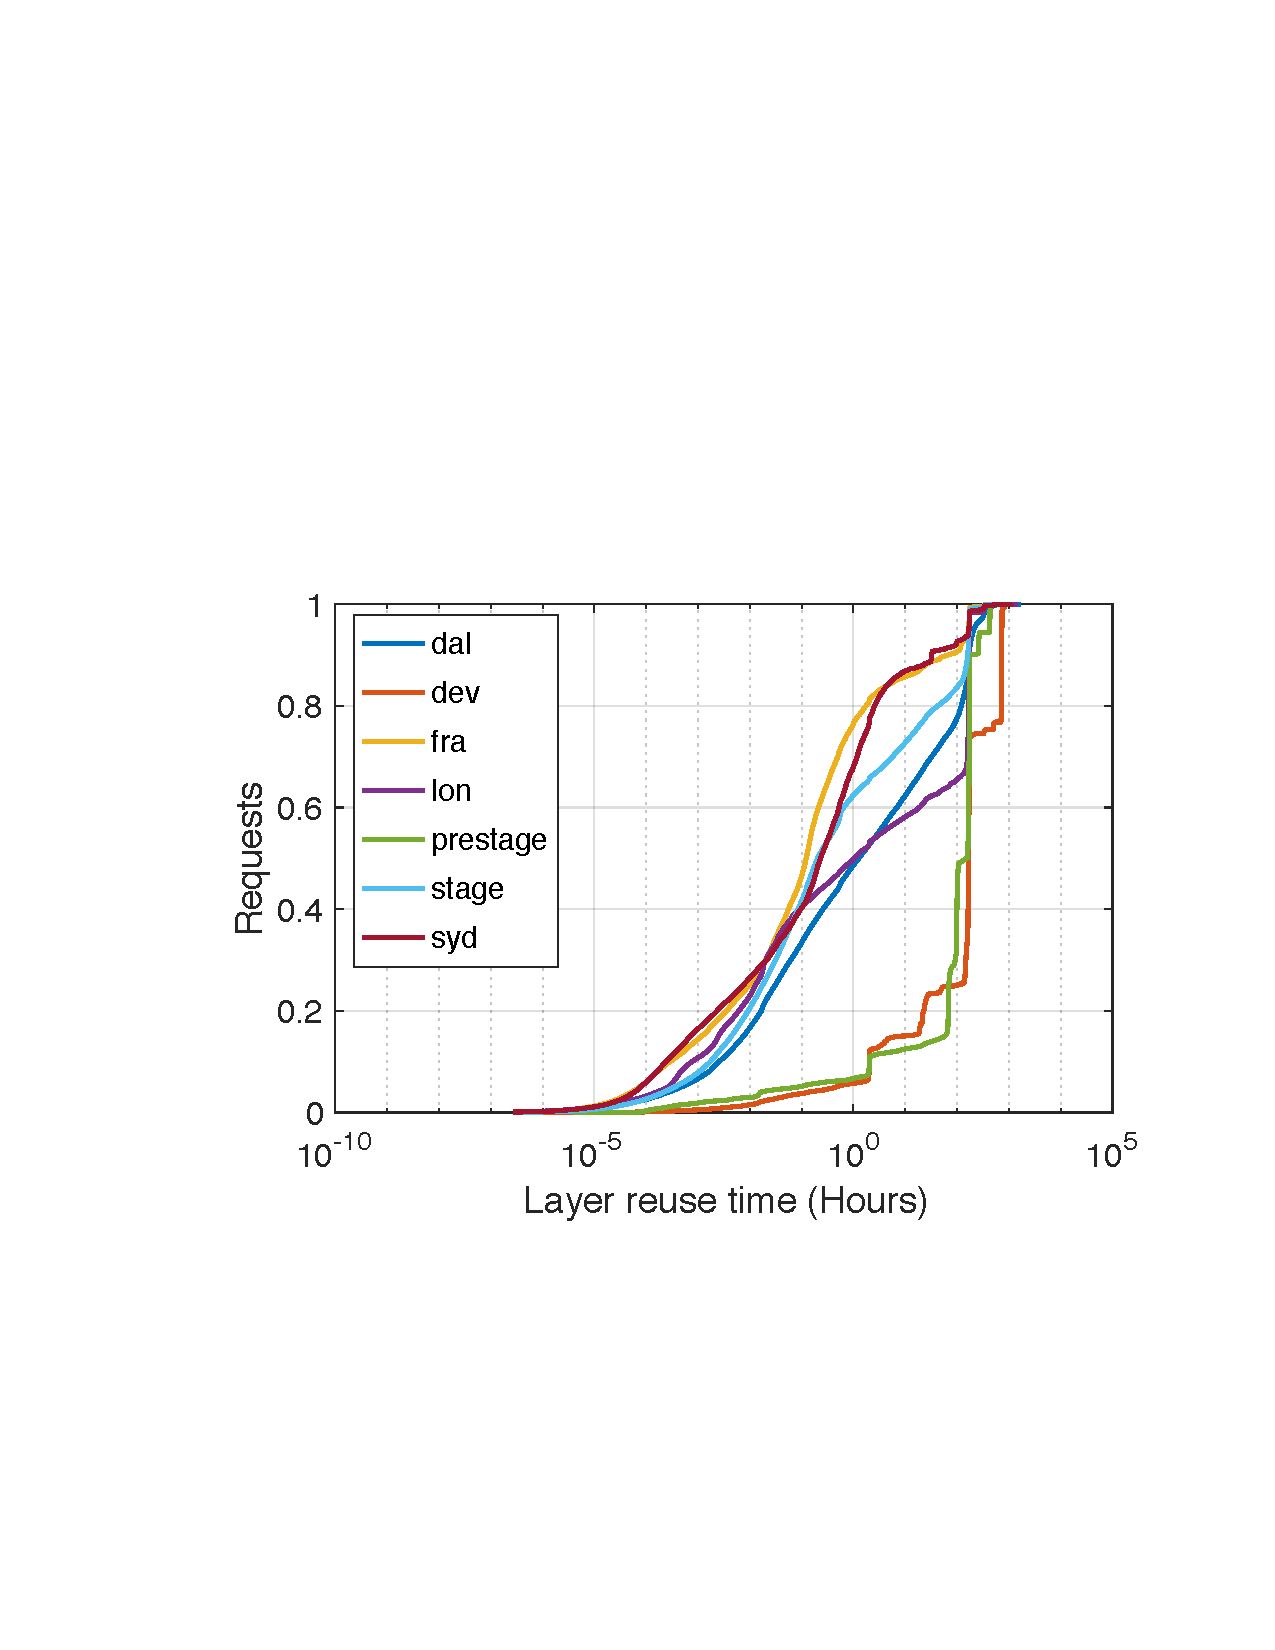
\includegraphics[width=0.2\linewidth]{graphs/layer-reusetime.pdf}
%			\label{fig:layer-reuse}
%	}
%	\subfigure[Repository repulling probability]{
%		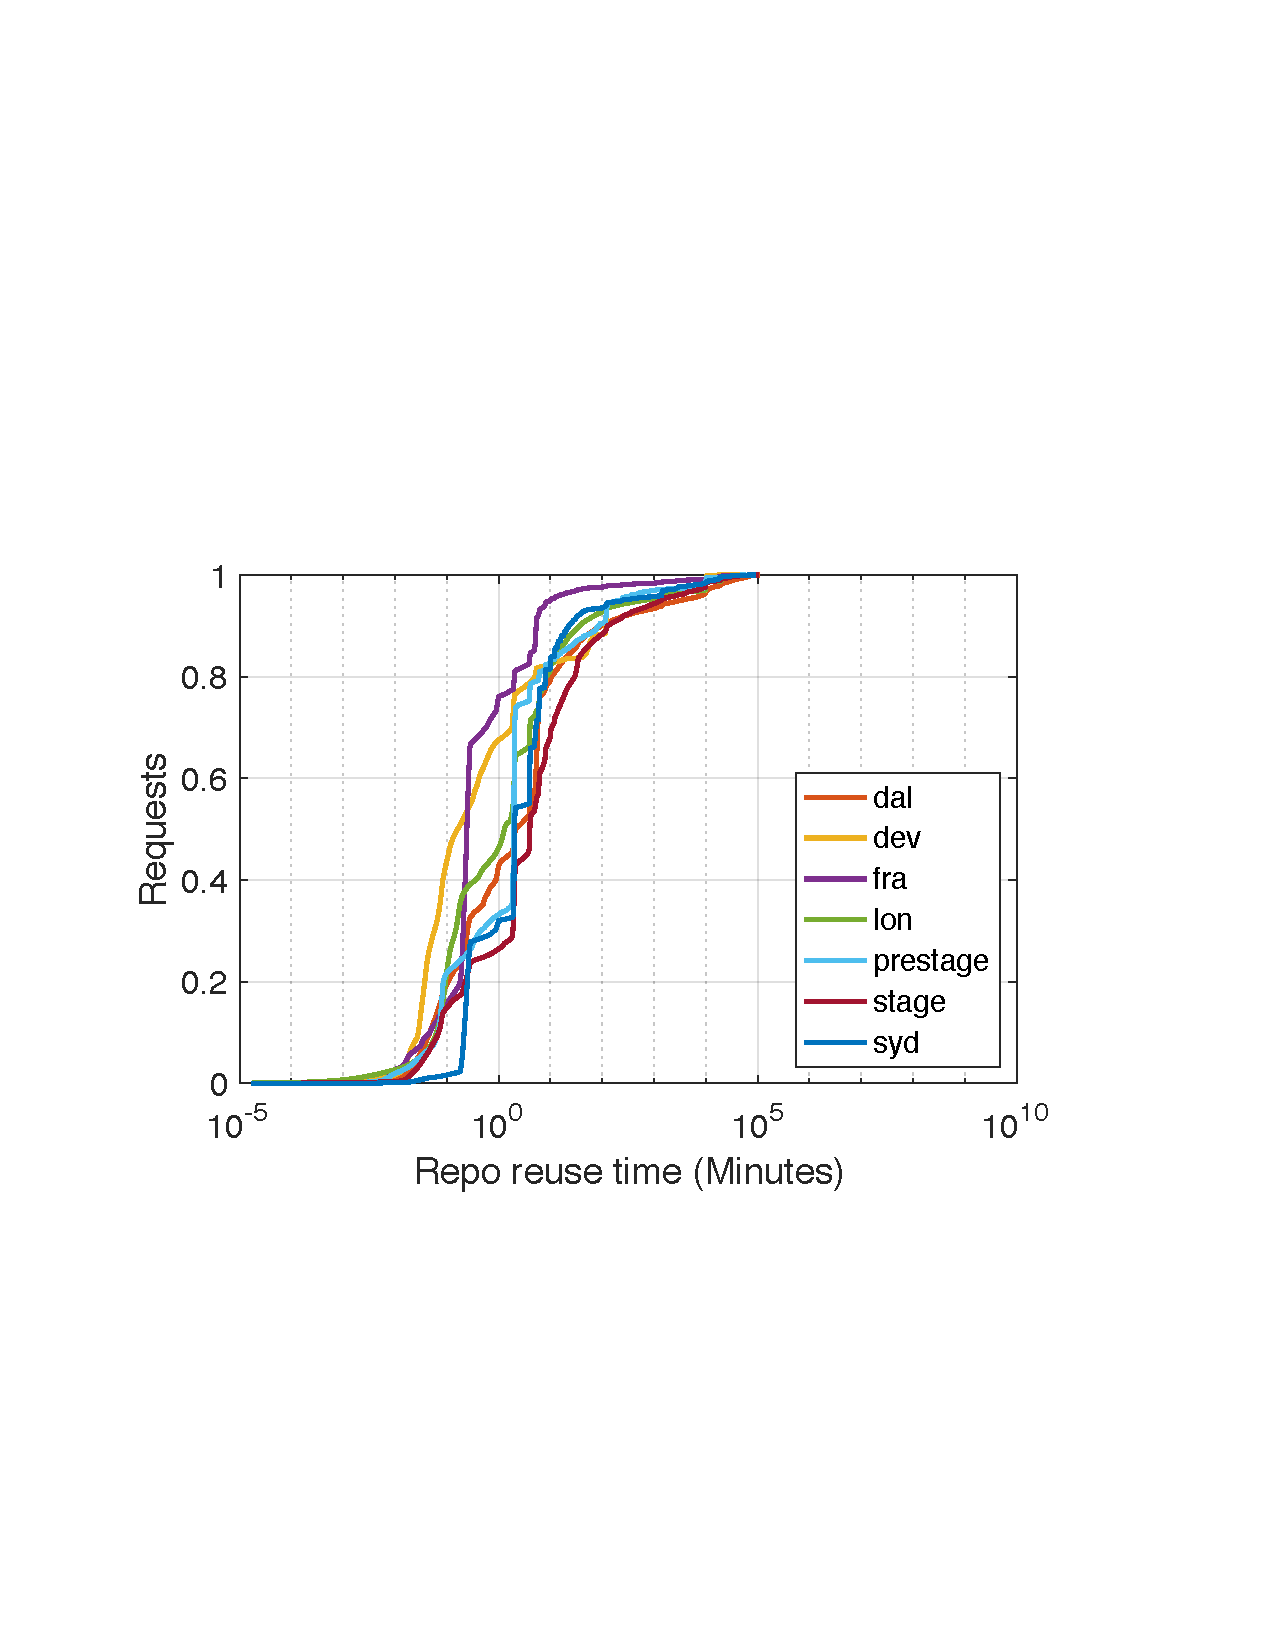
\includegraphics[width=0.2\linewidth]{graphs/repo-reusetime.pdf}
%				\label{fig:repo-reuse}
%	}
%	\subfigure[Client repulling probability]{
%		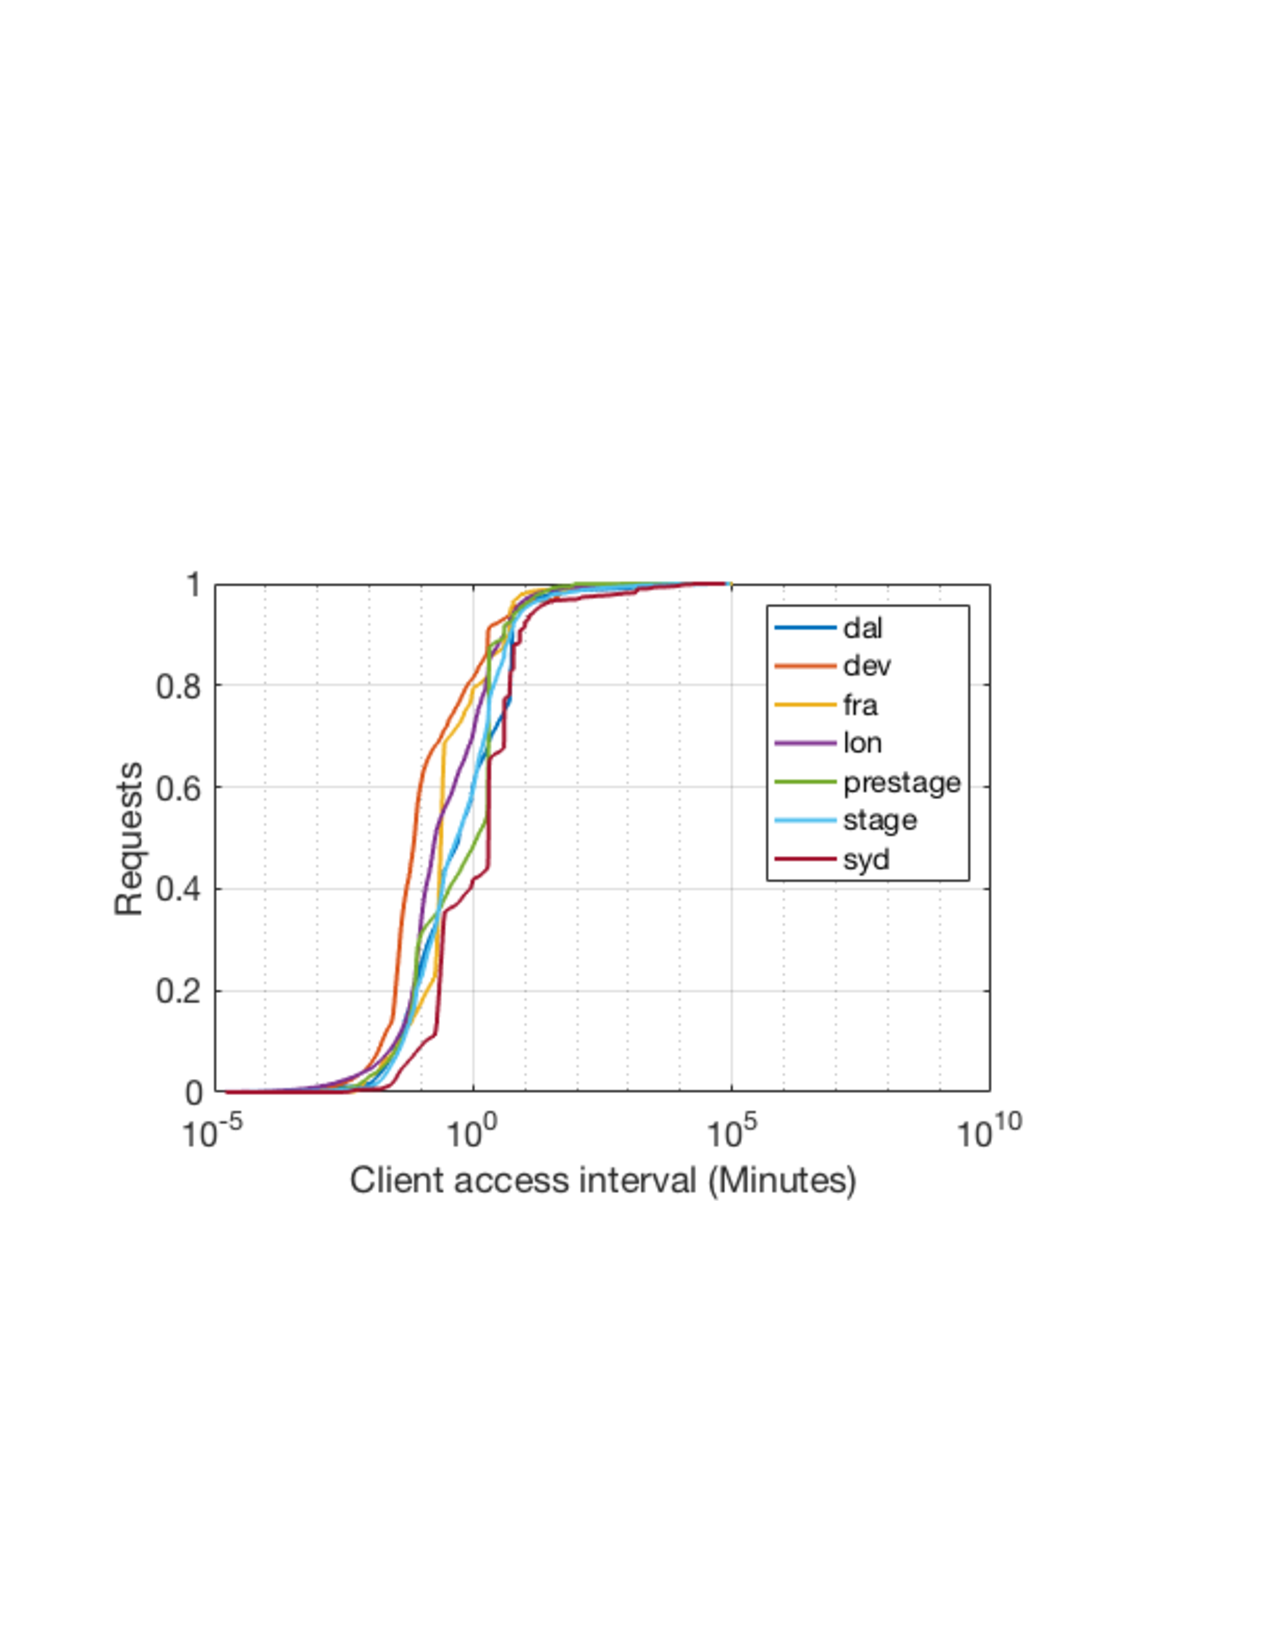
\includegraphics[width=0.2\linewidth]{graphs/user-intervals.pdf}
%			\label{fig:user-interval}
%	}
%	\caption{CDF of reusetime for layers, repositories and clients' access intervals.}
%	\label{fig:fig-reuse}
%\end{figure*}

%\begin{figure}[t]
%	\centering
%	\begin{minipage}{0.26\textwidth}
%		\centering
%		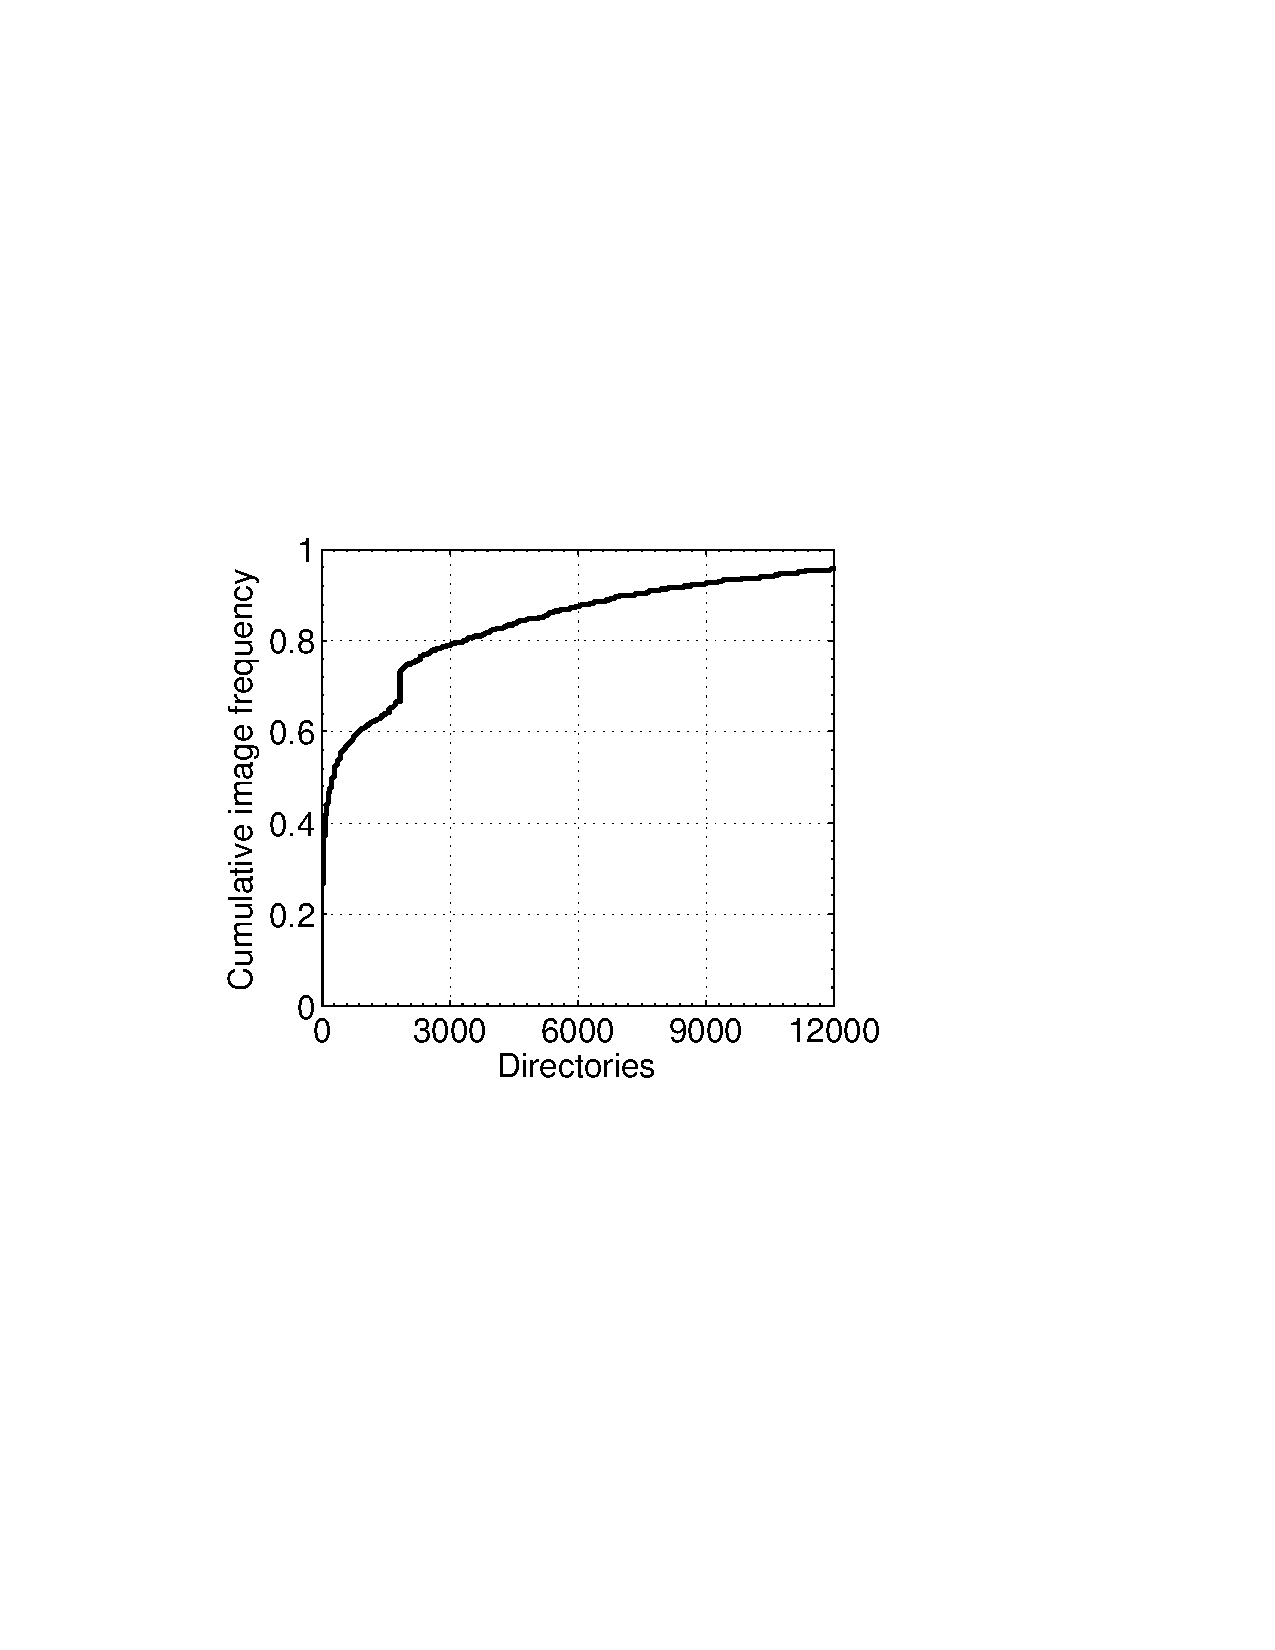
\includegraphics[width=1\textwidth]{graphs/dir.pdf}
%		\caption{CDF of images by\newline directories}
%		\label{fig-dir}
%	\end{minipage}%
%	\begin{minipage}{0.24\textwidth}
%		\centering
%		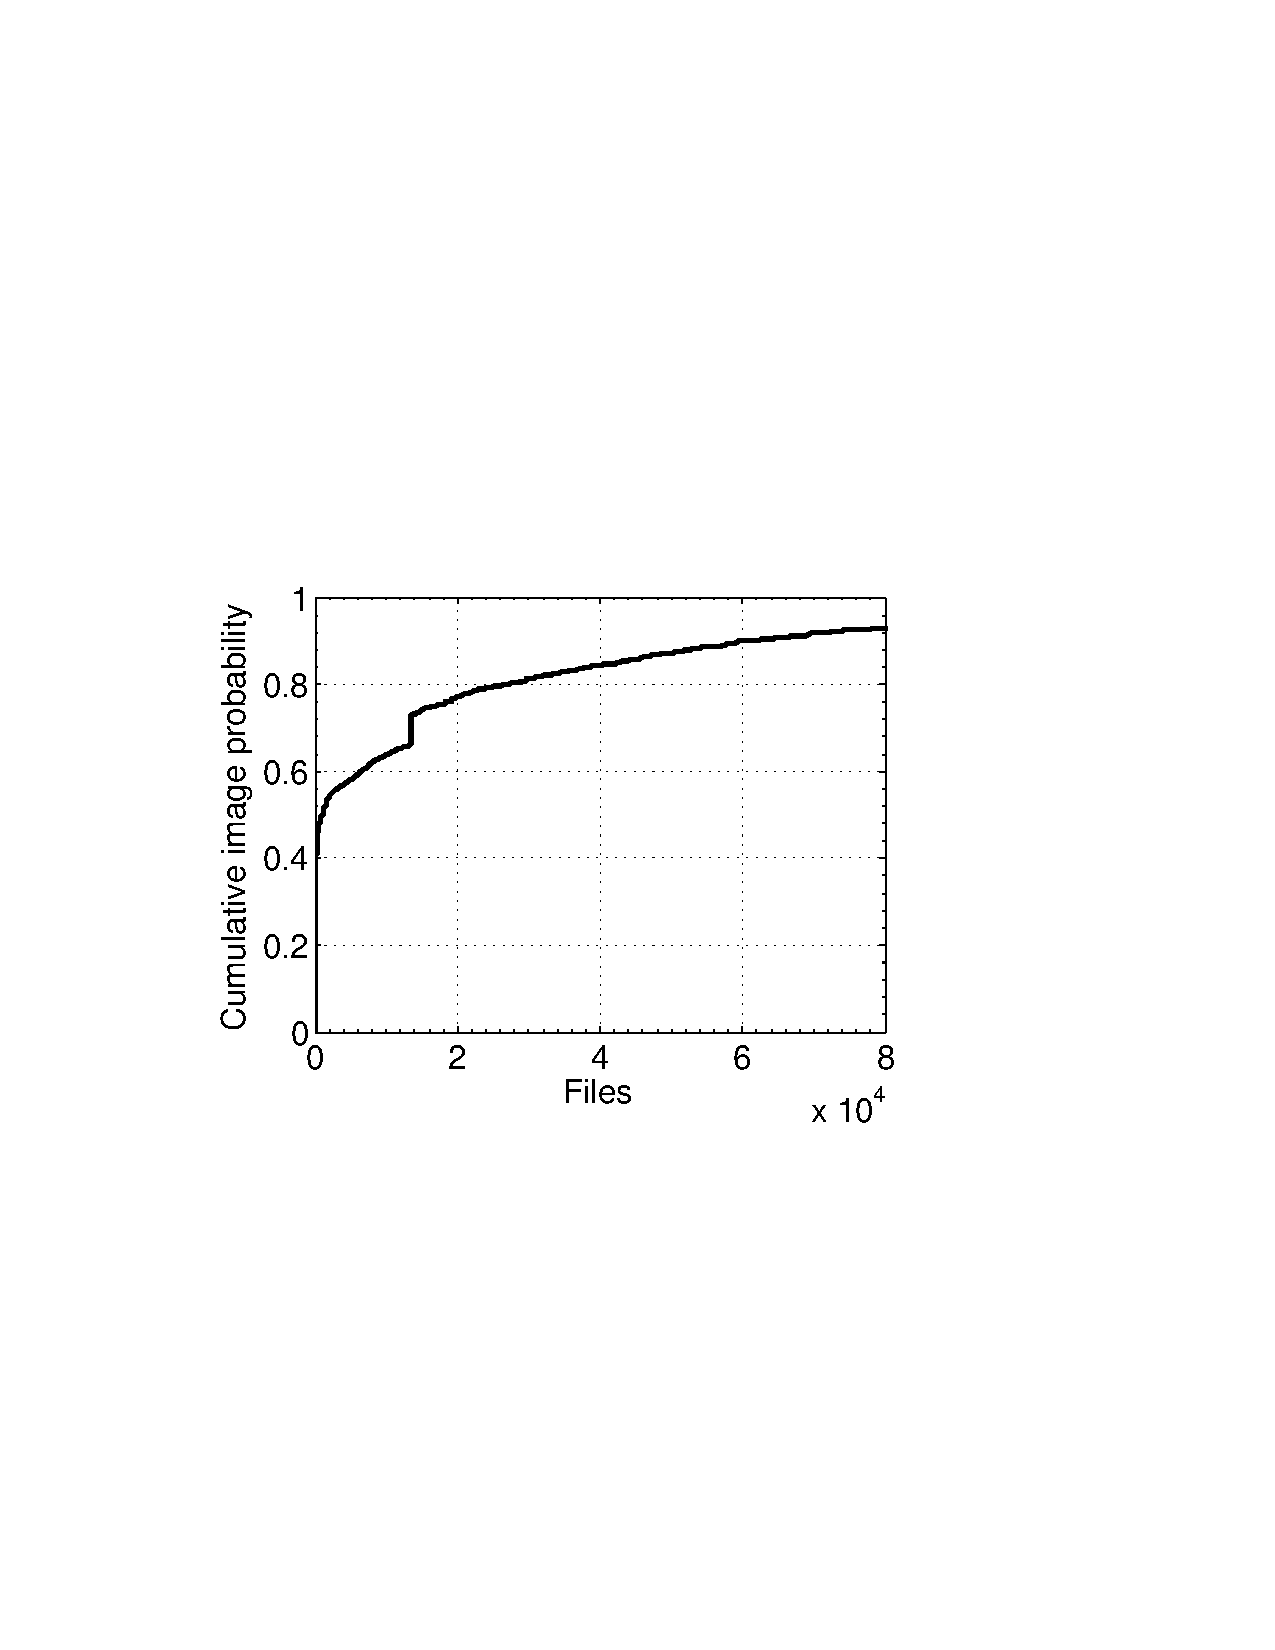
\includegraphics[width=1\textwidth]{graphs/file.pdf}
%		\caption{CDF of images by files}
%		\label{fig-file}
%	\end{minipage}
%\end{figure}

%\begin{figure}[htbp] 
%	\begin{minipage}{0.5\linewidth} 
%		\centering 
%		\includegraphics{circle} 
%		\caption{A Circle} 
%		\label{fig:circle} 
%	\end{minipage}% 
%	\begin{minipage}{0.5\linewidth} 
%		\centering 
%		\includegraphics{rectangle} 
%		\caption{A Rectangle} 
%		\label{fig:rectangle} 
%	\end{minipage} 
%\end{figure}
%
%As shown in~\cite{xxx},
%layer accesses are heavy skewed.
%There are hot layers that account for majority of layer accesses. 
%Hence, we can cache hot layers to improve performance.
Is it possible to 
preconstruct a layer before users pull a layer to save layer restoring latency?
We analyze the duration between a \texttt{pulling} manifest request and the subsequent \texttt{pulling} layer requests
and show in Figure~\ref{fig:intervals}.
We see that 
majority of intervals are greater than 1 s.
For example, 80\% of intervals from \texttt{lon} are greater than 1 s.
60\% of intervals from \texttt{syd} are greater than 5 s.
Hence,
there is a relatively long gap between a \texttt{pulling} manifest request and the subsequent \texttt{pulling} layer requests.
This is because, first,
when fetching an image from registry,
Docker client \emph{downloads} a certain number layers in parallel (3 by default)
starting from the lowest or base layers.
In this case, if the image contains more than 3 layers, then the \emph{upper} layers have to 
wait til the \emph{lower} layers are downloaded, which varies
\texttt{pulling} layer request arrive time on registry.
Second, network delay between clients and registries 
often accounts for a greater proportion of pulling latency in Cloud environment, especially for
large layers.
Consequently,
we can use this long gap to predict which layers will be pulled by the user
when a \texttt{pulling} manifest request is received,
 and then 
rebuild a layer for the user before \texttt{pulling} layer requests arrive.

%majority of \texttt{pull} layer requests access only few layers.
%\paragraph{Skewness}
%Figure~\ref{fig:layer-skewness} shows the CDF of layer popularity.
%We observe a heavy layer access skewness for \texttt{Fra}, \texttt{Syd}, \texttt{Dal}, \texttt{Stage}, and \texttt{Lon} with 60-80\%  of the \texttt{pull} layer requests accessing only 10\% of layers.
%Figure~\ref{fig:repo-skewness} shows the CDF of repository popularity.
%Compare to layer popularity, 
%repository access skewness is heavier across 7 workloads.
%Almost 90\% of \texttt{pull} layer requests access only 10\% of repositories for 
%\texttt{Dev}, \texttt{Fra}, \texttt{Prestage}, \texttt{Syd}, and \texttt{Stage}.
%Figure~\ref{fig:client-skewness} shows the CDF of client popularity.
%\texttt{Dal}, \texttt{Dev}, \texttt{Fra}, \texttt{Lon}, \texttt{Prestage}, and \texttt{Stage} shows a heavy client access skewness with
%10\% of clients send 95\% \texttt{pull} layer requests for \texttt{Lon}.
%Overall, caching a layer with higher pull count will improve the hit ratio, 
%especially for popular repositories and targeting active clients with higher repulling probability.
%
%\paragraph{Reuse time}
%Next, we analyze the layer and repository reuse time.
%Layer reuse time means the duration between two consecutive requests to the same layer
%while repository reuse time means the duration between two consecutive \emph{pull} manifest requests to the same repository.
%Figure~\ref{fig:layer-reuse} shows the CDF of layer reuse time. 
%%Layer reuse time means the duration between two consecutive \texttt{pull} requests to the same layer.
%We see that layer reuse time distribution varies among different workloads.
%For \texttt{Fra}, \texttt{Syd}, and \texttt{Stage},
%half of the layers' reuse time is shorter than 6 minutes.
%Half of layers from \texttt{Dal} and \texttt{Lon} have a reuse time higher than 1 hour and is higher than 100 hours for \texttt{Prestage} and \texttt{Dev}.
%Consequently, for \texttt{Dal}, \texttt{Lon}, \texttt{Prestage}, and \texttt{Dev}, 
%it may take longer than 1 hour for at least half newly requested layer to get a hit. 
%These layers shouldn't be cached since their reuse time is too long and may cause other useful layers or slices to be evicted, called \emph{cache pollution}.
%%Consider popular skewness, 
%Figure~\ref{fig:repo-reuse} shows the CDF of repository reuse time.
%%Repository reuse time means the duration between two consecutive \texttt{pull manifest} requests to the same repository.
%We see that repository reuse time is much shorter than layer reuse time.
%80\% of repositories are requested within 2-12 minutes across the 7 workloads.
%Figure~\ref{fig:user-interval} shows the CDF of client access intervals.
%client access interval means the duration between two consective requests issued by the same client.
%Client access intervals are much shorter than repository reuse time.
%80\% of client are active within 1 - 3 minutes for the 7 workloads. 
%Hence, to eliminate \emph{cache pollution},
%we consider the reuse time of layer and repository as well as client access intervals during cache eviction.

%<<<<<<< HEAD
%=======
%\paragraph{Skewness.}
%Figure~\ref{fig:layer-skewness} shows the CDF of layer popularity.
%We observe a heavy layer access skewness for \texttt{Fra}, \texttt{Syd}, \texttt{Dal}, \texttt{Stage}, and \texttt{Lon} workloads with $60$-$80$\%  of the \texttt{pull} layer requests accessing only $10$\% of the layers.
%Figure~\ref{fig:repo-skewness} shows the CDF of repository popularity.
%Compared to layer popularity, 
%repository access skewness is heavier across all the 7 workloads.
%Almost $9$\% of \texttt{pull} layer requests access only $10$\% of repositories for 
%\texttt{Dev}, \texttt{Fra}, \texttt{Prestage}, \texttt{Syd}, and \texttt{Stage}.
%Figure~\ref{fig:client-skewness} shows the CDF of client popularity.
%\texttt{Dal}, \texttt{Dev}, \texttt{Fra}, \texttt{Lon}, \texttt{Prestage}, and \texttt{Stage} show a heavy client access skewness. 
%For example, only $10$\% of clients issue $95$\% of the \texttt{pull} layer requests in the \texttt{Lon} workload.
%Therefore, caching a layer with a high pull count will improve the hit ratio, 
%especially for popular repositories and targeting active clients with high repulling probability.
%
%\paragraph{Reuse time.}
%Next, we analyze the layer and repository reuse time.
%Layer reuse time means the duration between two consecutive requests to the same layer
%while repository reuse time means the duration between two consecutive \emph{pull} manifest requests to the same repository.
%Figure~\ref{fig:layer-reuse} shows the CDF of layer reuse time. 
%%Layer reuse time means the duration between two consecutive \texttt{pull} requests to the same layer.
%We see that layer reuse time distribution varies among different workloads.
%For \texttt{Fra}, \texttt{Syd}, and \texttt{Stage},
%half of the layers' reuse time is shorter than $6$ minutes.
%Half of layers from \texttt{Dal} and \texttt{Lon} have a reuse time higher than $1$ hour and it is higher than $100$ hours for \texttt{Prestage} and \texttt{Dev}.
%Consequently, for \texttt{Dal}, \texttt{Lon}, \texttt{Prestage}, and \texttt{Dev}, 
%it may take longer than $1$ hour for at least half newly requested layers to get a hit. 
%These layers should not be cached since their reuse time is too long and may cause other useful layers or slices to be evicted, \ie causing \emph{cache pollution}.
%%Consider popular skewness, 
%Figure~\ref{fig:repo-reuse} shows the CDF of repository reuse time.
%%Repository reuse time means the duration between two consecutive \texttt{pull manifest} requests to the same repository.
%We see that repository reuse time is much shorter than layer reuse time.
%$80$\% of repositories are requested within $2$-$12$ minutes across all the 7 workloads.
%Figure~\ref{fig:user-interval} shows the CDF of client access intervals.
%client access interval refers to the duration between two consecutive requests issued by the same client.
%Client access intervals are much shorter than repository reuse time.
%$80$\% of client are active within $1$-$3$ minutes for the 7 workloads. 
%Hence, to eliminate cache pollution,
%we consider both the reuse time of layer and repository as well as client access intervals during cache eviction.
%
%\subsection{Layer Deduplication}
%
%\paragraph{Redundant files shared among layers.}
%Consider that deduplication incurs a performance overhead and the current Docker registry already stores layers in compressed format to save space and network transfer overhead. We first analyze the space efficiency of a registry that performs decompression and file-level deduplication and compare it to a registry that naively stores compressed layers.
%
%In Figure~\ref{fig:cacheefficiency}, the x-axis values correspond to the sizes of 5 samples of registry data of varying sizes with traditional layer compression. For a traditional registry, the compressed layer tarballs will be kept as is.
%While a registry with file-level deduplication will store \emph{deduplicated} layers (i.e., unique files). 
%The y-axis shows how much space a registry with file-level deduplication can save over compressed layer tarballs.
%For the first two samples of the dataset, with size less than $20$~GB, 
%there is no benefit to \emph{deduplicate} layers because the deduplication ratio is very low.
%However, when the dataset size is $200$~GB and over, we can save over $40$\% of space. Saved space increases almost linearly with the size of the layer dataset.
%This affirms the benefit of deduplicating layers as the registry size increases.
%
%\paragraph{Layer preconstruction.}
%>>>>>>> 94daa3df1d5d977ac11fd9da2aea7b4eed340be2
%\subsubsection{User access pattern based preconstruction}
%
%Docker client stores images as lists of layers and layers are shared among different repositories, 
%which is similar to Docker registry.
%When a client pulls an image from a repository, 
%it will first \texttt{pull} the manifest of the image~\cite{docker}~\cite{dockerworkload} and 
%parse the manifest to get the layer digests,
%then lookup each layer digest against a \emph{local layer index}.
%After that it only pulls the layers that have \emph{not been stored locally}.
%Theoretically, clients only pull layer once. 
%However, some clients may delete several local images and \emph{repull} layers for these images.
%%Moreover, kubernetes allows users always \emph{repull} layers no matter these layers locally available or not~\cite{docker}.  
%Here, a \emph{repull layer} indicates a layer a user pulls multiple times,
%and a \emph{non-repull layer} means users only pull this layer once.
%
%\preconstructcachename~starts parallel slice restoring for layers 
%when a \texttt{pull manifest} request is received, 
%which is called layer preconstruction.
%These preconstructed layer slices are temporally stored in the cache for later \texttt{pull slice} requests.
%In this case, slice restoring process and its overhead can be avoided if the requested slice is found in the cache.
%Next, we analyze user access patterns to identify which layers in the repository will be pulled by users after 
%\texttt{pull manifest} requests.



%\paragraph{Monitor user access patterns}
%To monitor user access patterns,
%\preconstructcachename~first uses a RLmap to record repository-layer relationship.
%If user~\emph{u} \emph{pushes} a  layer~\emph{l} to a repository~\emph{r},
%\preconstructcachename~will add an new entry (\emph{l}) in RLmap denoted as RLmap[\emph{r, l}]. 
%%Based on user access patterns,
%\preconstructcachename~ also maintains a URLmap for keeping track of user access patterns.
%To identify a user, 
%we extract \emph{user end host address} (\emph{r.client}) from each request (\emph{r}). 
%Each URLmap entry maintains a user profile for each user \emph{u} denoted as URLmap[\emph{u}]. %as shown in Figure~\ref{xxx}.
%User profile contains a list of repository profiles for each accessed repository \emph{repo} denoted as URLmap[\emph{u, repo}],
%and each repo profile contains a list of layer profiles for each accessed layer \emph{l}  denoted as URLmap[\emph{u, repo, l}].
%Note that layer profiles can be shared among different repo profiles for the same user.
%If user~\emph{u} \texttt{pull}s a layer~\emph{l} from a repository~\emph{repo},
%\preconstructcachename will update layer profile URLmap[\emph{u, repo, l}] with the corresponding layer repull count, and calculate
%repository repulling probability and user repulling probability for the corresponding repository profile and user profile.
%Each node records the following history information: (\emph{Get\_cnt}, \emph{Put\_cnt}, \emph{last\_access\_time}). a child node layer~\emph{L} to parent node~\emph{R}
%User profile records the user repulling probability $u.rp$ for client $u$.
%If $u.rp$ is greater than threshold $\theta_{crp}$, this user has a high probability of repulling layers.
%Repo profile records repository repulling probability $u.r.rp$ for repository $r$.
%If $u.r.rp$ is greater than threshold $\theta_{rrp}$, this repository is a popular repulling repository for this user.
%Layer profile records layer repull count $u.l.R$ for layer $l$.
%If $u.l.R$ is greater than threshold $\theta_{R}$, this layer is a popular repull layer for this user.



%\subsubsection{User access pattern  based cache replacement}

%
%\preconstructcachename~starts cache eviction when free space is low.
%To decide which layer or slices need to be evicted to make space for new requests,
%we analyze the temporal trend of user accesses as follows.



\section{\sysname~Design}
\label{sec:Sift}

%Our analysis in Section~\ref{sec:redundant_files} suggests that adding the
%support of file-level deduplication to Docker registry can significantly reduce
%its storage capacity requirements, especially in large-scale deployments.
%
%In this section, we first describe a high-level design of \emph{\sysname}---
%a Docker registry that supports file-level deduplication.
%We then proceed with a simulation-based evaluation of the expected performance
%implications.
%Integrated Caching and Deduplication
%Cache-assisted Inline deduplication system


%In this section, we first present the challenges brought by the unique characteristics of the Docker ecosystem.
%Next, we discuss our design goals and finally present the design of~\sysname. 
%Then we present the design of~\sysname. 
%O are to improve Docker registry performance and to decrease the backend storage requirements such as ???.

In this section, we present an overview of \sysname.
Then, we present how \sysname performs layer deduplication and layer restoring. 
Finally, we present our user-behavior based layer preconstruct cache (\preconstructcachename).
%a latency aware deduplication system (\dedupname system) and
\vspace{-4pt}
\subsection{Overview}
\label{sec:design}
\vspace{-4pt}

\begin{figure*}[t]
	\centering
		%\begin{minipage}{0.225\textwidth}
			\centering
			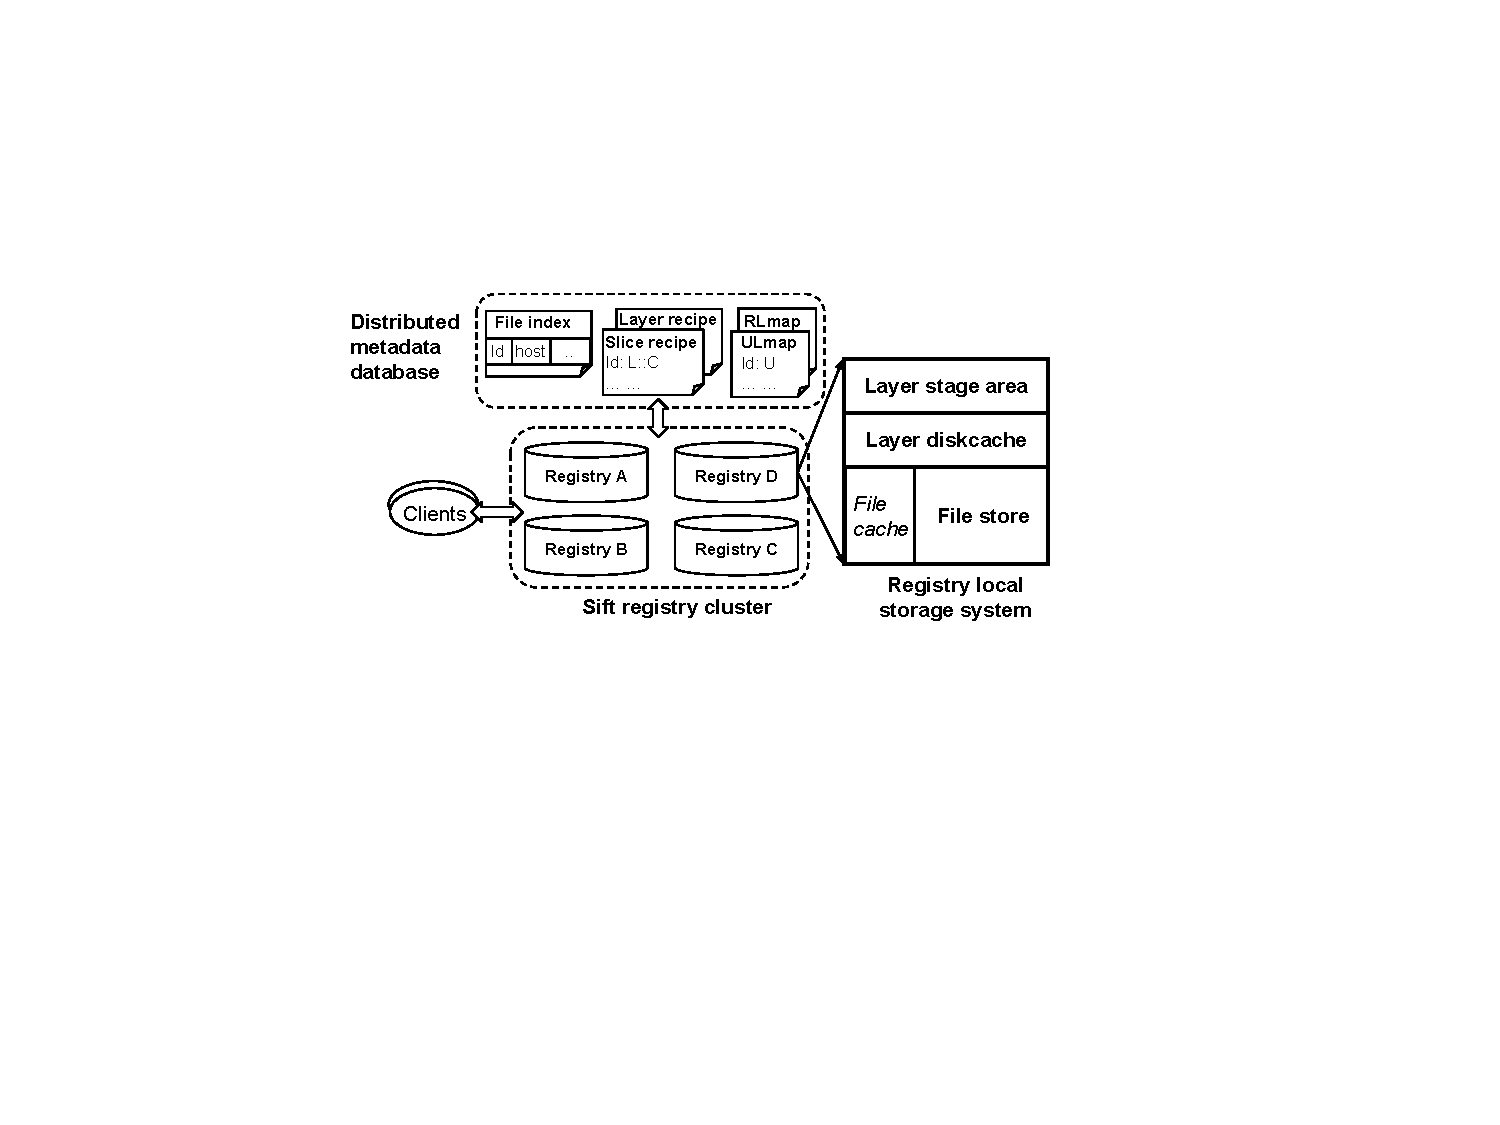
\includegraphics[width=0.9\textwidth]{graphs/sys-architecture.pdf}
%\vspace{-4pt}
			\caption{Architecture of \sysname.}
			%\label{fig:ref_count}
		%\end{minipage}
%	\begin{minipage}{0.225\textwidth}
%		\centering
%		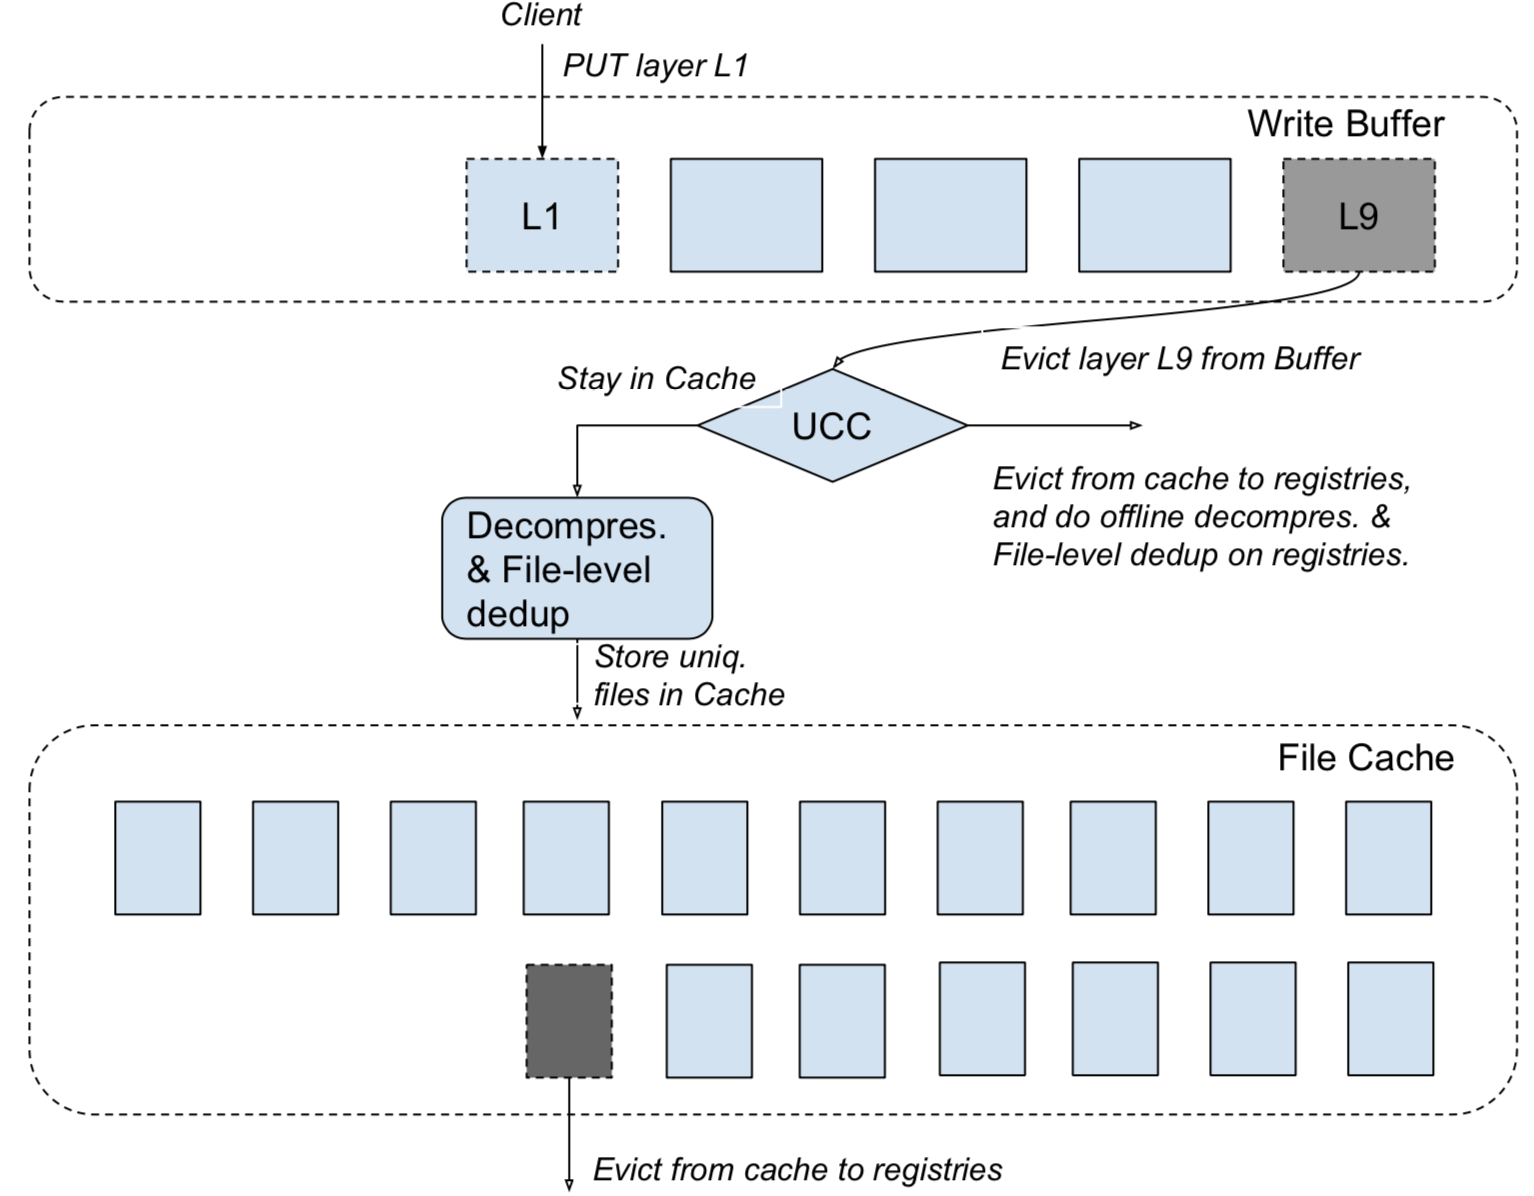
\includegraphics[width=1\textwidth]{graphs/slimmer-cache.png}
%		\caption{CDF of compress. and uncompress. layer size.}
%		\vspace{-3pt}
		\label{fig:sys-overview}
%\vspace{-4pt}
%	\end{minipage}
\end{figure*}


Figure~\ref{fig:sys-overview} shows the architecture of \sysname.
 \sysname is comprised of a distributed registry cluster and a distributed metadata database.
 Layers are stored on registry cluster and 
Metadata, such as Docker image manifests, are stored on distributed NoSQL databases for 
reliability, consistency, and fast accesses.
Each \sysname~registry consists of a user behavior based layer preconstruct cache (\preconstructcachename),
and a layer restoring latency aware deduplication (\dedupname) system.

In the following, we describe how Docker clients interact with \sysname.
\paragraph{Push}
As shown in Figure~\ref{fig:sys-overview}, client \textit{A} creates a new hello-world image
\texttt{hello-world:new}
from the official image which only contains a single layer \textit{L1}
by 
committing
the modifications over \textit{L1} as a new layer \textit{L2}.  
When client \textit{A} pushes \texttt{hello-world:new} to the registry,
it only pushes the new layer \textit{L2} to the registry since registry already stores \textit{L1}.
When \sysname~receives \textit{L2}, 
it first cache \textit{L2} in \preconstructcachename~for later accesses,
and at the same time, 
\sysname~will also submit \textit{L2} to the backend storage system as shown in Figure~\ref{fig:sys-overview}.
\preconstructcachename~ uses write through policies. 
Since there is no modification to the layer, 
there is no data consistency issue between the cache and the backend storage system.
Next, client \textit{A} pushes a new manifest \textit{M1:0} to the registry and finish image pushing.
As shown, \textit{L2} is added to the manifest \textit{M1:0} for image \texttt{hello-world:new}.


\dedupname~process runs periodically to deduplicate compressed layer tarballs (detailed in~\cref{sec:dedup-desgin})
into unique files to save storage space.
As shown in Figure~\ref{fig:sys-overview}, cold layer \textit{L2} is selected to be deduplicated.
\dedupname~process decompresses \texttt{L2} and removes the duplicated files from \emph{uncompressed} \texttt{L2}.
After that, \dedupname~process evenly distributes the unique files to the registry servers.
In this case, each server stores a \textbf{deduplicated slice} of \texttt{L2}, from which a layer \textbf{slice} of \texttt{L2}
can be constructed.
We define all the per-server files belonging to a layer as a {\em deduplicated slice}. 
A server stores deduplicated slices for many layers, 
and a layer is composed of \emph{slices} 
that can be restored from the deduplicated slices stored on multiple servers, 
which allows restoring a layer in parallel. 
To do that, 
\dedupname~process uses copy-on-write to update the old manifest \textit{M1:0} by adding slices' digests into it 
and generates new manifest \textit{M1:1} as shown in Figure~\ref{fig:sys-overview}.
Slice digest is calculated by hashing slice content~\cite{xxx}.

\paragraph{Pull}

As shown in Figure~\ref{fig:sys-overview},
when client \textit{C} pulls an official image \texttt{hello-world} from registry,
\sysname~first check if the requested layer \textit{L1} presents in~\preconstructcachename.
If so, the \texttt{pull} layer request will be served by cache.
Otherwise, \dedupname~process starts parallel slice restoring process.
For example, when client \textit{B} pulls image \texttt{hello-world:new} from registry,
\sysname~sends the latest manifest \textit{M1:1} to client.
After receiving the \textit{M1:1}, client \textit{B} first parses \textit{M1:1} and get a list of slice digests for \textit{L2}.
Instead of sending ``\texttt{pull layer L2}'' request, client will send multiple ``\texttt{pull slice of L2}'' requests to registry.
As shown, client \textit{B} sends ``\texttt{pull slice S1}'', ``\texttt{pull slice S2}'', and 
``\texttt{pull slice S3}'' to the registry 
since \textit{L2} is comprised of \textit{S1} , \textit{S2}, and \textit{S3}.
These requests are forwarded to the servers that stores corresponding deduplicated slice of \textit{L2}.
%On \sysname~side, \textit{L2} is stored as deduplicated slices distributed among different servers.
The servers will start to restore slices from local deduplicated slices and send individual slices back to client 
in parallel as shown in Figure~\ref{fig:sys-overview}. 
When client \textit{B} receives all the slices, it decompresses them together as an uncompressed layer.

\paragraph{Docker client modifications}
 
To interact with \sysname, Docker client is modified to 
parse \sysname~manifest with additional attributes -- slice digests.
If slice digests present in a layer object in the manifest JSON file, 
client will replace ``\texttt{pull layer} request with multiple ``\texttt{pull slice}'' requests.
Besides, when client receives slices back from registry, 
it decompresses these slices together into an uncompressed layer.  
%When a user requests a
%layer that is not present in the layer buffer, the request is forwarded to the
%file cache (detailed in~\cref{sec:design_operations}). 
%If a layer is also not found in the
%file cache, the request is forwarded to the backend dedup storage system.
%Note that after layer deduplication, unique files are
%scattered across multiple servers. 
%We define all the per-server files belonging to a layer as a {\em slice}. 
%A server stores slices for many layers, and a layer is composed of slices stored on multiple servers.
%To avoid the network latency caused by fetching slices from different servers and
%assembling them into a whole compressed layer, we split a \texttt{pull} request 
%into several~\texttt{pull slice}~requests. Those requests will then be
%forwarded to all the backend servers that store the requested
%layer's slices. 
%After a~\texttt{pull slice}~request is received, each backend server compresses the slice 
%and directly sends it back to the user.
%We modify the Docker client
%interface such that when it receives all the compressed slices, it can
%decompress them into a single layer. 
%Furthermore, compressing slices in parallel considerably lowers the layer compression latency,
%since compression time depends on the size of the
%uncompressed data.
%to cache layers and cache unique files after decompression and deduplication,
%respectively.  consists of a \emph{layer buffer} and a \emph{file cache}.  The
%layer buffer stores all the newly pushed layers in memory.  Although accessing
%memory is very fast, the size of main memory is limited. 
%All the slices for a layer are fetched in parallel for performance improvement.






%\sysname~seamlessly integrates 
%%the management of 
%caching and deduplication on the
%backend storage system (\emph{backend dedup storage}) with Docker registries.
%%
%We address a set of unique challenges to enable this integration.
%%
%First, for caching layers, \texttt{pull} layer requests are difficult to
%predict because layers are accessed infrequently.
%In~\cref{sec:background},
%%\arb{???}, 
%we have observed that about half of the layers are not
%accessed again for at least $1.3$~hours. Which means that if we
%cache a layer, we may need to wait a long time before we observe a hit on that layer.  %(as discussed in~\cref{sec:background}).  
%This is mainly 
%because when a user pulls an image from the registry, the Docker daemon on the
%requesting host will only pull the layers that are not locally stored.
%%\Ali{I do not understand the following sentence.}
%%Moreover, we have to consider that a user might deploy an applications on
%%multiple machines, so it's not easy to predict when a user will access which layers. 
%%%\Ali{The above statement is incorrect. You have to distinguish between GET layer requests
%%that are issued after a (PUSH layer + GET manifest) request and a normal GET layer request.
%%FAST paper only talk about case 1. Whereas you are generalizing that any GET layer request
%%should have a precedent GET layer request which is wrong. We can make a case
%%that not all GET layers requests have a precedent PUSH layer request but we can
%%not say that it takes a few days, weeks, or even months for a user to make a pull
%%layer request after a push layer request.}
%%\NZ{I mean the first case, push beyond your trace collection time.}
%%
%
%Second, we can not deduplicate compressed layers. For deduplication, each layer
%needs to be uncompressed, and only then can undergo file-level deduplication. Similarly,
%to restore a layer, we need to fetch files from multiple servers, and only then compress
%them in to a tar file to serve a \texttt{pull} layer request. 
%%\arb{that can service the ??? request}\NZ{addressed}. 
%This whole process can incur a 
%considerable performance overhead on \texttt{pull} layer requests.
%Deduplication also slows down
%\texttt{push} layer requests because of its high demand for CPU, memory, I/O, and network resources.
%%\Ali{Explain how push layer requests are not effected?}\NZ{fixed}
%
%%\subsection{Design}
%To address these issues, we propose a new registry design. The key feature of our design is a user-access-history-based prefetch algorithm that helps mitigate the performance degradation due to the 
%backend dedup storage system (Figure~\ref{fig:sys-overview}). Based
%on layer access pattern we observed in~\cref{sec:background} and user access history information,
%\sysname precisely prefetch the layers that may be pulled shortly.
%%has not been pulled in the requested repository
%%and the prefetched 
%%In this case, we can   
%%a user's active time is predictable. 
%%Thus, we leverage users' behavior, \ie
%%when a user is most likely to be active, to drive layer evictions from the cache.
%
%
%%\begin{figure}[t]
	\centering
		%\begin{minipage}{0.225\textwidth}
			\centering
			\includegraphics[width=0.4\textwidth]{graphs/fig-sift-manifest}
%\vspace{-4pt}
			\caption{\sysname~manifest.}
			%\label{fig:ref_count}
		%\end{minipage}
%	\begin{minipage}{0.225\textwidth}
%		\centering
%		\includegraphics[width=1\textwidth]{graphs/slimmer-cache.png}
%		\caption{CDF of compress. and uncompress. layer size.}
%		\vspace{-3pt}
		\label{fig:sys-overview}
%\vspace{-4pt}
%	\end{minipage}
\end{figure}
%
%Considering that layer sizes are typically about several MB~\cite{dockerworkload}, 
%a small main memory cache will be unable to accommodate
%all prefetched layers for all active users. 
%To address this issue, we 
%create separate caches for layers and \emph{unique} files, called {\em layer buffer} and {\em file cache}, respectively. 
%%Both caches comprise both
%%main memory and flash memory.
%%Layer buffer
%%\arb{are main memory for one type and flash for the other type, or both for both types. I assumed both types of memory are used, and there are two caches. check previous sentence for correctness.}\NZ{addressed}
%Note that, layers are  compressed tarballs and buffered in layer buffer, and 
%%sent by users
% \emph{unique} files are uncompressed files from which duplicates have been removed and stored on flash-based storage. 
%%We call compressed layer cache and \emph{deduped} files cache,
%%\emph{layer buffer} and \emph{file cache}, respectively.
%For 
%cache evictions, we first evict inactive users' layers from the layer buffer.
%Next, we \emph{dedup} the evicted layers, then store the \emph{unique} files
%into the file cache (detailed in~\cref{sec:design_operations}). 
%%the following operations: decompressing each evicted layer and comparing its
%%containing files with the files that are already stored in the file cache,
%%eliminating duplicate files, that is, only storing the unique files on flash
%%storage.



 


\subsection{Deduplicating layers}
\label{sec:dedup-desgin}

%Next, we explain in detail, how \sysname stores and deduplicates layers.
%
%\subsubsection{Layer replication, deduplication, and partitioning}
%
As in the traditional Docker registry, \sysname maintains a \emph{layer index}.
After receiving a \texttt{PUT} layer request,
\sysname first checks the layer fingerprint in the \emph{layer index} to ensure 
an identical layer is not already stored.
%The layer fingerprint is calculated by hashing the layer content 
%and serves as the layer ID.
If not, \sysname,
replicates the layer $r$ times across the P-servers
and submits the remaining $R-r$ layer replicas to the D-servers. Those replicas are
temporarily stored in the layer stage areas of the D-servers. \sysname uses
two consistent hashing rings to for each cluster to pick the target servers for
a layer. Once the replicas
have been stored successfully, \sysname notifies the client of the request completion.
%
%\LR{How are the target D- and P-servers selected? Through consistent hashing?} 
%\NZ{In our current implement, we distribute layers to D- and P-servers
%by using two CHT rings: a ring of D-server and a ring of P-servers.}

% and acknowledges back to the client.
%
%
%After the layer is deduplicated, it will be removed from stage area.
%\dedupname system~initiates layer deduplication process only if 
%layer deduplication will achieve significant space savings and 
%the process won't impact foreground requests. 
%Sepcially, layer deduplication process is triggered when
%the layer dataset $S$ is greater than a predefined threshold $\theta_{s}$ and 
%the registry traffic $RPS$ ( i.e., requests per second) is lower than $\theta_{RPS}$. Thus, layer deduplication process runs periodically.
%The process always stars with the cold layers that haven't been
%access for a long time.
%
% After D-servers receive the layer replicas,
% replicas will be temporally saved into layer stage areas as shown in Figure~\ref{fig:sift}.
%

%\sysname then initiates the deduplication process, which runs \emph{off-line} to not affect \texttt{push}
%latencies. Deduplication is only performed once by a single D-server for a single layer replica
%and the resulting unique files are then replicated to achieve the desired replica count.
%which collaborates with the metadata database
%to remove redundant files from layers. 
%Note that only one layer replica is selected from the submitted $R-r$ replicas on D-servers to do layer deduplication.
%After decompressing the layer, the deduplication process consists of three main steps: 
%layer decompression, 
%1)~file-level deduplication;
%2)~unique file replication; and
%3)~layer partitioning. 
%The first two steps are necessary for removing duplicate files from compressed layer tarballs
%and reliably store the remaining unique files.
%
%\LR{Need to make this more clear. Are we just deduplicating one layer but then copy the
%resulting unique files to $R-r$ D-servers?}
%The last step is needed
%to evenly distribute unique files for a layer across D-servers to balance the I/O and computational load
%during layer reconstruction while maintaining fault-tolerance.  

%After the layer replica is \emph{deduplicated}, all the backup layer replicas stored on D-servers in the layer stage area will be discarded.  

%The last two step -- file replication and layer partitioning is 
%to evenly distribute the I/O and computation load of layer restoring across multiple registry servers 
%while also maintaining a level of redundancy.  
%Note that only one layer replica is selected among $R-r$ layer replicas to do layer deduplication. % subil: NEED CLARIFICATION ON WHAT THIS MEANS
%After that, all the layer replicas will be discarded.  
%>>>>>>> ab86d0a4767bfcfcbb58baf9bd7b2e81e54d7e51
%This makes the process of layer restoring achieve the maximum parallelism for each layer to accelerate the restoring process. 
%(detailed in~\cref{subsubsec:slice-restoring}) 
%After layer deduplication, unique files are evenly distributed across multiple registry servers. 

%%\begin{figure*}[t]
%		\begin{minipage}{0.21\linewidth}
%			\centering
%			\includegraphics[width=1\textwidth]{graphs/dedup_vs_compression.pdf}
%			\caption{File-level deduplication vs. compression efficiency.}
%		%	\vspace{-3pt}
%			\label{fig:cacheefficiency}
%		\end{minipage}
%			\begin{minipage}{0.38\linewidth}
%				\centering
%				\includegraphics[width=1\textwidth]{graphs/sift-metadata.pdf}
%				\caption{Metadata for deduplication.}
%				%	\vspace{-3pt}
%				\label{fig:sift-metadata}
%			\end{minipage}
%		\begin{minipage}{0.38\linewidth}
%			\centering
%			\includegraphics[width=1\textwidth]{graphs/restoring-breakdowns.pdf}
%			\caption{Breakdown of slice restoring time.}
%			%	\vspace{-3pt}
%			\label{fig:slice-restoring-breakdown}
%		\end{minipage}
%\end{figure*}

\begin{figure}[t]
	\centering
	\centering
	\includegraphics[width=0.45\textwidth]{graphs/sys-architecture-put-layer.pdf}
	\caption{Layer deduplication. \LR{Typo: ``Hearder'' should be ``Header''}}
	\label{fig:dedup-partition}
\end{figure}



%\begin{figure}[t]
%	\centering
%	\begin{minipage}{0.26\textwidth}
%		\centering
%		\includegraphics[width=1\textwidth]{graphs/dir.pdf}
%		\caption{CDF of images by\newline directories}
%		\label{fig-dir}
%	\end{minipage}%
%	\begin{minipage}{0.24\textwidth}
%		\centering
%		\includegraphics[width=1\textwidth]{graphs/file.pdf}
%		\caption{CDF of images by files}
%		\label{fig-file}
%	\end{minipage}
%\end{figure}

%\begin{figure}[htbp] 
%	\begin{minipage}{0.5\linewidth} 
%		\centering 
%		\includegraphics{circle} 
%		\caption{A Circle} 
%		\label{fig:circle} 
%	\end{minipage}% 
%	\begin{minipage}{0.5\linewidth} 
%		\centering 
%		\includegraphics{rectangle} 
%		\caption{A Rectangle} 
%		\label{fig:rectangle} 
%	\end{minipage} 
%\end{figure}

%\begin{figure}[t]
	\centering
%		\begin{minipage}{0.23\textwidth}
%			\centering
%			\includegraphics[width=1\textwidth]{graphs/evaluation_hitratios.png}
%			\caption{Hit ratio.}
%			\label{fig:hitratio}
%		\end{minipage}
	%	\begin{minipage}{0.25\textwidth}
			\centering
			\includegraphics[width=0.4\textwidth]{graphs/sift-metadata.pdf}
			\caption{Metadata for deduplication.}
			%\vspace{-3pt}
			\label{fig:sift-metadata}
	%	\end{minipage}
\end{figure}
\paragraph{File-level deduplication}
%\LR{Is the following just how the .tar format is structured or are we doing anything
%additional to the headers and the content? If not, we should just mention that this is
%how tar is creating archives.}
%
%As shown in Figure~\ref{fig:dedup-partition},
Following the staging area, \sysname
uncompresses the layer and passes the decompressed tar file to the deduplication process.
%In this process, 
%the layer tarball is first decompressed into a \textbf{layer tar archive}~\cite{xxx}.
%Algorithm~\ref{alg:dedup-partition} details layer deduplication and partitioning. 
%After layer decompression, 
Each file entry in the archive is represented as a \emph{file header} and the associated
\emph{file content}~\cite{basictar}.
The file header contains metadata such as file name, path, size, mode, owner information, etc.
%
%and is needed to correctly rebuild the \emph{file header} for 
%the associated file entry in the restoring layer archive.
%
\sysname records every file header in slice recipes (described below)
to be able to correctly restore the complete layer archive later.
%
%
%##### need to record all files in the tar archive, not just unique files' header but also the deduplicated
%files'headers. otherwise, how do you restore a complete tar achieve?????
%
\sysname computes the file Id for each file by hashing the file content and 
checks, whether the file Id is already present in the file index.
If the file Id is already stored, the file content will be discarded. 
Otherwise, it will be saved physically in the D-server's file store and 
the file Id is recorded in the file index.%
% As shown in Figure~\ref{fig:replication-partition},
The file index maps different file Ids to the physical file replicas stored
on different D-servers.
%represented as a file location and a file size.
%File location is denoted as 
%Besides, each file Id in the file index is also mapped to its \emph{host address} with the associated \textbf{backup level}.
%Backup level denotes whether the host stores a primary backup file replica (i.e., \texttt{P}) or the $n^{th}$ backup replica (ie., \texttt{B}\emph{n}) detailed as follows.
%detailed as following.

%\LR{Here, we need to explain in more detail, what exactly a slice is (just a collection of headers?),
%how a header is linked to its file content, and how files/headers are linked to layers (through layer
%recipe? We should also talk a little bit about our metadata overhead here.}

\paragraph{Unique file replication}
%
%Note that, layer deduplication process only deduplicates regular files., 
%
Next,
\sysname replicates and distributes unique file replicas across D-servers.
%Hence, the layer partitions on D-servers can be used to restore a \emph{slice} of layer in parallel.
%To speedup layer restoring process,
%\sysname distributes file replicas and 
%in a way such that
%each server is able to rebuild an $\sim$equal-sized slice of the layer from its local file store.
%
%As mentioned earlier, \sysname records every file header from a layer tar archive.
%Sift will hold on to the file headers from tar archive to be included as part of the slice recipe.% \Subil{The previous sentence seems to indicate that the header-contentpointer pairs are stored in the D-server. But they are only stored in the metadata database as part of the slice recipe, right?}
%\NZ{yes}
The headers and content pointers of all the files, in a given D-server, that belong to a particular layer are included in that D-server's \emph{slice recipe} for that layer.
%(see Figure~\ref{fig:replication-partition}). 
%After unique file replication and layer partitioning,
After file replication, \sysname adds the new slice recipes to the metadata database.
%A slice recipe represents a layer slice and is used to construct a
%\emph{partial layer archive}.

\sysname also creates a \emph{layer recipe} for the uploaded layer and stores it in the metadata database.
%as shown in Figure~\ref{fig:replication-partition}.
The layer recipe records all the D-servers that store slices for that layer and which can act
as \emph{restoring workers}. When a layer needs to be reconstructed,
one worker is selected as the \emph{restoring master}, responsible 
for gathering all slices and rebuilding the layer~(see~\S\ref{sec:restore-desgin}).

Figure~\ref{fig:replication-partition} demonstrates how Sift pipeline operates.
The example assumes B-mode 1 with 3-way replication, i.e. each unique file has two replicas distributed
on two different D-servers.
The files $f1$, $f2$, and $f3$ are already stored in \sysname,
and $f1'$, $f2'$, and $f3'$ are their corresponding backup replicas.
Layer $L1$ is being pushed and contains files $f1$, $f2$, $f3$, $f4$, $f5$, and $f6$. 
%is decompressed and \emph{file-level deduplicated}.
$f1$, $f2$, and $f3$ are \emph{shared files} by $L1$ and other layers, and hence,
are discarded during file-level deduplication.
%\emph{f1, f2,} and \emph{f3} are shared by \emph{L1} and other layers, denoted as \textbf{shared files}.
The unique files $f4$, $f5$ and $f6$ are added to the system and
replicated to D-servers $A$, $B$, and $C$.
%We describe how the target servers are chosen later in this section.

After replication, server $B$ contains $f2$, $f5$, $f1'$, and $f4'$. Together
$f2$ and $f5$ form the \emph{primary slice} of $L1$, denoted as $L1::A::P$.
This slice Id contains the layer Id the slices belongs to ($L1$), the node, which
stores the slice ($A$) and the backup level ($P$ for primary).
%\todo{explain this notation}.
%\NZ{This slice Id contains the layer Id it belongs, the host server, and the backup level of this slice.
%This slice Id notation largely simplifies layer recipe and facilitate layer restoring.
%The restoring master only needs to fetch a small layer recipe, get the restoring workers,
% and decide which backup level slices are needed for layer restoring.
% After that, the master sends out simple layer restoring instructions to the workers.
% The layer restoring instruction only contains the layer Id and the backup level.
%The workers will generate a slice Id by using the layer Id and backup level
%along with its own address, which holds the slice stored locally.}
%
%shared file replica \emph{f2} and 
%unique file replica \emph{f5} stored on \emph{B} comprise a slice of \emph{L1},
%denoted as a \textbf{primary slice} of \emph{L1} (ie., \emph{L1::A::P}).
The two backup file replicas 
$f1'$ and $f4'$ on $B$ form the \emph{backup slice} $L1::B::B$.
During layer restoring, $L1$ can be restored by using any combination of primary and backup slices
to achieve maximum parallelism.
%
%\LR{Why are \emph{f4'} and \emph{f8'} only a backup slice?}
%\LR{Instead of putting the fX in emph environments, we should use math mode and put numbers in the index, e.g.
%$f_{4}'$.}

%=======
%After discarding duplicate files
%, the deduplication process distributes the layer's remaining files across different registry servers
%so that each server is able to build an $\sim$equal-sized % subil: is the \sim necessary?
% slice of the layer from its local file store when needed.
% We define the collection of files that belong to a layer as a \emph{slice} of that layer stored on the registry server. 
%A server stores slices for many layers, and a layer is composed of slices stored on multiple servers, which allows restoring a layer in parallel. 
%Finally, \sysname will add slice recipes and layer recipe to metadata database as shown in Figure~\ref{fig:dedup-partition}.
%
%Figure~\ref{fig:replication-partition} shows an example of file replication and layer partition.
%Each file has two replicas distributed on different servers,
%\emph{r1, r2, r3,} and \emph{r4} are four primary file replicas that were already stored in the system.
%and \emph{r1', r2', r3',} and \emph{r4'} are their associated backup file replicas. 
%A layer \emph{L} that contains files \emph{r1, r2, r3, r4, r5, r6, r7,} and \emph{r8} is pushed.
%Files \emph{r1, r2, r3,} and \emph{r4} are deduplicated
%while new files
%\emph{r5, r6, r7,} and \emph{r8} will be added to the system, 
%As shown, \emph{r5, r6, r7,} and \emph{r8} are replicated and distributed to registry \emph{A, B, C,} and \emph{D} 
%as primary file replicas and backup file replicas.
%Consequently,
%primary file replicas \emph{r1} and \emph{r5} stored on registry \emph{A} comprise one of layer \emph{L'}s slices, 
%denoted as \textbf{primary slice}:
%\emph{layerid:A}.
%The two backup file replicas \emph{r4'} and \emph{r8'} stored on registry \emph{A} comprise a \textbf{backup slice} for the primary slice stored 
%on registry \emph{D} (i.e., \emph{r4} and \emph{r8}).
%>>>>>>> ab86d0a4767bfcfcbb58baf9bd7b2e81e54d7e51

%primary file replicas
\begin{figure}[t]
	\centering
	\centering
	\includegraphics[width=\columnwidth]{graphs/replication.pdf}
	\caption{Layer dedup, replication, and partitioning.}
	\label{fig:replication-partition}
\end{figure}

%\begin{algorithm}
\scriptsize 
	\caption{Layer deduplication and partitioning}
	\label{alg:dedup-partition}
	\KwIn{\\	
			$FileIndex$: File index. \\
	}

	\KwOut{\\
			$LayerRecipe$: Layer recipe for layer $L$.\\
			$SliceRecipes$: Slice recipes for layer $L$' slices.\\
	}

	archive $\leftarrow$ \texttt{Decompress} layer $L$ \\

	\ForEach{header, content in archive} 
	{ 
		Id $\leftarrow$ \texttt{Hash} content \\
		%destHeader $\leftarrow$ header \\
		\eIf{ Id in FileIndex}{
			host  $\leftarrow$ $FileIndex$[Id].host \\
			src $\leftarrow$ $FileIndex$[Id].header \\
			{\tiny\texttt{/* SliceRecipe is identified by `layerid::host'}}
			SliceRecipe[$L::host$] $\leftarrow$  \texttt{Add} (header, src) \\
			{\tiny\texttt{/* Skip redundant file.  }}\\
		}{
			{\tiny\texttt{/* create file with content in file store.  }}\\
			file $\leftarrow$ \texttt{Create and write} content \\
			src $\leftarrow$ \texttt{Stat} file \\
			entries $\leftarrow$ (header, src)  \\
		}
	}
	
	\Do{entries}{
		{\tiny\texttt{/* get file entry with maximum file size. }}\\
		maxFile $\leftarrow$ \texttt{Max} entries \\
		{\tiny\texttt{/* get smallest slice. }}\\
		minSlice $\leftarrow$ \texttt{Min} SliceRecipes \\
		{\tiny\texttt{/* assign biggest file to smallest slice. }}\\
		minSlice $\leftarrow$ \texttt{Add} maxFile \\
		{\tiny\texttt{/* Set maxFile to FileIndex}}\\
		{\tiny\texttt{/* Remove maxFile from entries. }}\\
	}
	{\tiny\texttt{/* Send slices.}}\\
	{\tiny\texttt{/* Set SliceRecipes.}}\\
	{\tiny\texttt{/* Include all slices' hosts to workers.}}\\
	{\tiny\texttt{/* Select biggest slice' host as master.}}\\
	{\tiny\texttt{/* Set LayerRecipe.}}\\
	
	
		
\end{algorithm}




%<<<<<<< HEAD
%Then, the process sends slices to the corresponding registries.
%Slice is identified by a simple combination of the layer id and its host address 
%with the associated backup level,
%denoted as $layerid::host::backuplevel$. % as shown in Algorithm~\ref{alg:dedup-partition}.
%As shown in Figure~\ref{fig:replication-partition},
%the primary slice stored on \emph{A} is denoted as \emph{L::}\emph{A::}\texttt{P}
%while the rest backup slice is denoted as \emph{L::}\emph{A::}\texttt{B2}.

%=======
%Algorithm~\ref{alg:dedup-partition} details layer deduplication and partitioning algorithm.
%After layer decompression, 
%each file entry in the layer archive % subil: what is the layer archive referring to?
% is represented as a \textbf{file header} and a \textbf{file content}.
%The file header contains the file name, path, size, mode, owner information, etc. % subil: should elaborate on structure of the header, how is it constructed?
%The file header is needed to rebuild the \emph{file header} % subil: how are the two file headers different?
%for 
%the associated file entry in the layer archive.
%
%%During layer deduplication process,
%\sysname records each file entry's file header and 
%calculates the file id by hashing the file content.
%As mentioned earlier, the file index maps a \emph{file id} to its associated physical file that is stored in the file store.
%To address a physical file,
%each file id in the file index holds its 
%%denoted by a combination of its 
%\emph{host address} and \textbf{file status} of the physical file which mainly contains file name, path, and size.
%As shown in Algorithm~\ref{alg:dedup-partition}, 
%if a file's id already exists in file index (i.e. it's present in a registry server), 
%this file will be added to its host's corresponding slice for that layer. 
%Otherwise,
%\sysname stores the file content as a physical file in the file store
%and retrieves the file status of the physical file.
%The file index is updated accordingly.
%
%The slice recipe is identified by a simple combination of the layer id and its host registry address,
%denoted as $layerid::host$ as shown in Algorithm~\ref{alg:dedup-partition}.
%A slice recipe represents a layer partition and
%is used to construct a partial layer,
%>>>>>>> ab86d0a4767bfcfcbb58baf9bd7b2e81e54d7e51
%which
%records each file entry' $header$ in the layer archive partition and 
%its corresponding physical file's status . 
%In this case, 
%each file is represented as a $header$ in the layer archive and
%its corresponding physical file's status $src$. 
%
%During layer deduplication process,
%After unpacking the layer archive, 
%
%Note that destHeader can be used to rebuild the \textbf{file header} for 
%associated file entry in the layer archive.
%
 %its host' slice
%to get identical files' server addresses.

%\LR{The following needs to be reformulated to be more clear.}
%
\paragraph{Layer partitioning}
To improve reconstruction times, it is important that different layer slices
are equally sized and evenly distributed across D-servers.
%The example in Figure~\ref{fig:replication-partition}
%shows such a perfect scenario, in which the files of layer $L1$ are evenly partitioned across all D-servers.
%since its shared files and unique files are evenly distributed to D-servers. 
%However, in general, it is not straightforward to evenly distribute shared files for different
%layers as their placement is fixed by the first layer, which was pushed to the registry that
%contained these files.
%\LR{Provide more details. Why is that so? Is this assuming consistent hashing?}
%\NZ{Let's consider an empty storage system, the first layer can be easily evenly partitioned
% to servers because no shared files are stored.
%After the first layer is partitioned and stored,
%consider that the second layer is pushed,
%the second layer has some same files with the first layer and
%these shared files are already distributed to servers.
%These shared files are distributed in a way such that the first layer can be evenly partitioned.
%But they might not be evenly distributed for the second layer because
%when we distribute files for first layer we dont know the subsequent layers and
%we dont know which files will be shared with the subsequent layers.
%So the shared files' layout will affect the subsequent layers' partition.}
%
%To evenly distribute and partition a layer's unique and shared files
%, shared and unique files,
%
%To distribute the newly added unique files' primary replicas,
To achieve this, \sysname employs a greedy packing algorithm.
%, which is constrained by  with shared file constraints.
%distribute the newly added unique files in a way such that
%each D-server stores relatively equal-sized slice for the layer.
%\LR{What exactly is meant by `shared file constraints'. Can we explain a bit more?}
%\NZ{It means before partition the layer, some of its containing files (shared files)
%are already allocated to the servers.
%We dont want to migrate those files to make all its containing files evenly distributed.
%So I called it a constrain.
%It means when we partition layers, we maintain its containing shared files that are already allocated
%and stored on servers as it is. 
%Through only distribute the newly added unique files,
%we achieve a relatively even partition for a layer.}
%
Consider first the simpler case in which each file only has
a single replica. During layer partitioning, \sysname does not migrate shared files that already
have been stored on D-servers to reduce I/O overhead.
%
%\LR{The following is unclear, why does \sysname partition shared files for $L1$? Aren't they already there?}
%\NZ{I think it's allocating not partitioning.}
%
%\sysname first partitions $L1$ shared files to their host servers.
%\sysname first determines the location of $L1$'s shared files in the cluster.
%For example, in Figure~\ref{fig:replication-partition}, shared files $f1$, $f2$, and $f3$ are located
%on D-servers $A$, $B$ and $C$ respectively. It then computes the total size of the shared files
%for each affected D-servers.
\sysname first computes the total size of the layer's existing shared files for each D-server (this could
potentially be 0 if a D-server does not store any shared files for the layer).
Next, \sysname 
%starts to assign unique files to D-servers following a greedy packing strategy.
assigns the biggest unique file to the smallest partition until all the unique files are assigned.
%In the example, the shared files are evenly partitioned to all three D-servers,
%and hence, the three newly added unique files are also evenly assigned to the three servers.
%Otherwise, the biggest unique files will be assigned to the smallest partitions.
%\LR{As a general note, it seems like we generate quite a bit of metadata to keep track
%of the slices etc. Are we planning to evaluate how much metadata we generate?}
%\LR{Here, we need to talk about how we are planning to address the problem of metadata management as
%we are manually assigning files to servers and hence, have to store the location of each file in an index.
%How do we scale? What if we are dealing with billions of files?}
%\NZ{We just add a server address for each file Id in the file index.
%As shown in implementation section,
%we store the unique files as: ‘rootdir/docker/registry/v2/uniquefiles/sha256/
% <first two hex bytes of file digest> /<hex file diges>t’ so that given a file digest, 
% we can build the file path to save metadata information.}
%Finally, \sysname updates the file index with the newly added unique files.

%\LR{The following is unclear and needs a better explanation. Are the new primary replicas
%assigned to servers which do not yet store shared files for the new layer? What if all
%servers already store at least one shared file for the layer? How are the backup replica
%servers picked?
%}
%\NZ{The shared files also have primary replica and backup replicas.
%Simply, we distributed the primary replica of newly added unique files
%according to the distribution of primary replicas of shared files.
%And we distributed the secondary replicas of newly added unique files
%according to the distribution of secondary replicas of shared files to maintain a relatively even partition.
%Moreover, we also make sure that the secondary replicas of a newly added unique file
%is not stored on the same server with its primary replica.
%So when we distribute the secondary replicas, we need to consider the 
%secondary replicas of shared files and the previously allocated primary replicas.
%}
%
In the case where a file has more than one replica, \sysname performs the
above described partitioning \emph{per replica}. That means that it first assigns
the primary replicas of the new unique files to D-servers according
to the location of the primary replicas of the existing shared files. It then assigns the secondary
replicas according to the location of the existing secondary replicas and so on.
Additionally, \sysname also ensures that two replicas of the same file are never
placed on the same node.

%Next, we consider the case that each file has multiple replicas. The file
%index contains the location of the primary and backup replicas for each shared file.
%%For each shared file, its file Id points to multiple file replicas in the file index as
%%shown in Figure~\ref{fig:dedup-partition}.
%When adding new unique files, \sysname first distribute the files
%according to the shared files' primary file replicas' partitions. After that,
%\sysname assigns the replicas of unique files onto different servers with their primary
%replicas.

%After layer partition,.
%All the primary slices' hosts are denoted as layer restoring \textbf{primary workers}. 
%Next, \sysname stores slice recipes in metadata database after successfully
%sending slices to their corresponding workers.
%\sysname selects the biggest slice' host as layer restoring \textbf{primary master}.
%Layer recipe records the primary workers and master information for layer restoring.
%After that, \sysname~distributes primary slices' corresponding backup slices.
%Their hosts are denoted as \textbf{backup workers}.
%Finally, \sysname stores layer recipe in metadata database.
%Layer recipe 

%Here, we use the metadata database as a distributed lock for file index.
%File index sets a file id to hold  only if the file id does not exists.

%it uses a weighted round robin algorithm to distribute newly added 
%unique files to the registry cluster. These servers that already contains this layer's identical files
%are assigned a lower weight. 
%This is to ensue that different servers maintain same amount of files that are needed to restoring equal sized 
%slices for this layer.
%Deduplication process also 
%updates the \emph{file index} with the newly added unique files' fingerprints and host addresses.   
%Then, it calculates the slice fingerprints and creates a slice recipe for each slice.
%Slice recipe contains partial of the layer tarball's directory tree structure, file fingerprints, file name along with file path in the tarball, and file metadata information 
%(such as permissions and creation date), which are needed for restoring a slice for the layer. 

%After that
%After removing the duplicate files,
%Then, it
%distributes the \emph{deduplicated slices} evenly to the registry cluster by using round-robin, and,
%In the end, deduplication process creates a layer recipe which contains its slices' fingerprints and 
%based on layer recipe, it updates image manifests.
%The layer's tarball and file duplicates are removed after deduplication.

%<<<<<<< HEAD
%\subsection{Layer restoring}
%\label{sec:restore-design}
%%\paragraph{Parallel slice restoring}
%%\label{subsubsec:slice-restoring}
%
%

\begin{figure}[t]
	\centering
	\centering
	\includegraphics[width=\columnwidth]{graphs/sift-layer-construct-new.pdf}
	\caption{Parallel streaming layer construction.}
	\label{fig:construct}
\end{figure}


%
%When a~\texttt{pull} layer request is received and its associated 
%P-servers fail, 
%\sysname will first search layer diskcache on D-servers.
%If not found,
%\sysname will rebuild the layer from file store according to its layer recipe. 
%%the \dedupname~system 
%%first prepares a directory structure for the slice, based on the slice recipe.
%%Then, it copies the files into the directory tree.
%%Next, it compresses the slice's directory tree into a slice tarball,
%%and directly sends it back to the client.
%
%\paragraph{Parallel layer construction}
%
%When a~\texttt{pull} layer request is received, 
%\sysname will update \emph{ULmap}. 
%ULmap records user access status,
%which maps a \textbf{user id} to its accessed layers with its corresponding access count,
%where user id is defined as client request address.
%
%Upon a \texttt{pull} layer request fails on P-servers,
%\sysname initiates a layer restoring process on D-servers for it.
%The process has two parts: slice constructor and layer constructor.
%Figure~\ref{fig:restoring} shows an example of parallel layer restoring when a \texttt{pull} layer request failure happens.
%First, 
%layer constructor fetches the layer recipe from metadata database.
%As shown in $L1$'s layer recipe, 
%the primary restoring workers contains registry $A$, $B$, and $C$.
%Since registry $A$ is the primary restoring master,
%\emph{A} sends ``\texttt{Get primary slice}" requests to its peer workers: $B$ and $C$.
%After a \texttt{Get primary slice} request is received, 
%$B$ and $C$ start primary slice construction and return a primary slice back to $A$ respectively.
%Meanwhile $A$ instructs local slice constructor to rebuild a primary slice for $L1$.
%Slice constructor first gets its associate slice recipe (``$L1::P:A$") from metadata database 
%keyed by a combination of  layer id, slice type (i.e., primary $P$ or backup $B \#$) and registry address.
%Then, based on slice recipe,
%slice constructor fetches files pointed by $Srcs$
%and builds a slice archive.
%After receiving all slices, layer constructor concatenates them into a compressed layer
%and sends back the client. 
%
%\paragraph{Streaming layer construction}
%Figure~\ref{fig:construct} details the stateless streaming layer construction process.
%First, slice constructor loads file in parallel from file store based on the slice recipe.
%Each file is written to an archive buffer asynchronously.
%Before writing file content to the archive buffer, slice constructor first builds and writes its
%associated 
%file header into the archive buffer according to the slice recipe. 
%After archiving all the files in the slice,
%the archive buffer will be divided into few chunks and compressed in parallel,
%then concatenated into a single compressed slice stream.
%Through network transfer, multiple slice streams will be concatenated into a single layer.
%No intermediate file will be created or stored on disk. % subil: whoa!
%\sysname uses a small file inmemory cache to reduce file I/Os. 
%File cache uses Adaptive Replacement(ARC)~\cite{xxx}.
%
%%headers according to $Dests$,
%%after that it writes file contents into the archive
% 
%%Slice restoring process has four suboperations: 
%%slice recipe lookup,
%%slice file copying,
%%slice compression, and
%%slice network transfer. 
%%To measure the overhead for each suboperation, 
%%we implemented layer deduplication and parallel slice
%%restoring on a 4-node registry cluster. 
%%We first warmup the cluster by pushing 200 layers to the cluster
%%and initiating layer deduplication process.
%%The layers were randomly selected from our layer dataset detailed in xxx limited to 50MB.
%%After finishing layer deduplication,
%%we sent 400 \texttt{pull slice} requests to the cluster with 10 \texttt{pull slice} requests issued at a time.
%%Figure~\ref{fig:slice-restoring-breakdown} shows the CDFs of the latencies for each suboperation.
%%We see that across the four suboperations,
%%the duration for slice compress is the shortest.
%%Slice compression only took less than 0.001 s because a slice is a smaller unit. 
%%The next shortest suboperation is network transfer since we pulled layer slice through Ethernet.
%%90\% of slice recipe lookups took less than 0.1 s while 
%%the highest slice recipe lookup duration almost reaches 0.8 s,
%%which is caused by high concurrent lookup requests 
%%%(note that we use redis to store metadata \NZ{use mongodb instead}).
%%The most time consuming suboperation is slice file copying, which involves 
%%copying all 
%%the files that belong to the slice to their destination directory based on the slice recipe.
%%Note that we implemented a thread pool on each registry server to read files in parallel
%%and write data in RAMdisk to reduce disk IOs.
%%40\%of slice file copying duration is greater than 1 s and 
%%10\% of slice file copying duration is higher than 10 s.
%%This is because bigger slices contains more files and requires more disk IOs.
%%The overhead of slice copying can be largely mitigated for a large-scale registry cluster
%%since the size of slice roughly equals to $S_{l}/N$, where $S_{l}$ denotes the layer size and $N$ is size of registry cluster.
%%However, it could be a bottleneck for slice restoring on a small-scale registry cluster.
%%%and slice file copying duration depends on slice size.
%%
%%%\begin{algorithm}
\scriptsize 
	\caption{File cache assisted slice restoring}
	\label{alg:file-cache}
	\KwIn{\\
		$\theta_{rsfc}$: Slice restoring latency threshold. \\
		$s$: Slice to be restored. \\
	}

	\SetKwFunction{Fsub}{Restore}
	\SetKwProg{Fn}{Function}{:}{}

	\Fn{\Fsub{s}}{
		%{\tiny\texttt{/* Otherwise, it's a repull layer miss   /}}\\
		\eIf{files in s are cached in file cache}
		{
			slice $\gets$ \texttt{RestoreSlice} \emph{s} \texttt{From} \emph{file cache + disk} 
		}
		{
			slice, $D_{rs}$ $\gets$ \texttt{RestoreSlice} \emph{s} \texttt{From} \emph{disk} \\
			\If{ $D_{rs} > \theta_{rsfc}$} 
			{ 
				\emph{file cache} $\gets$ \texttt{Cache} \texttt{Subsetof} \emph{s.files}
			}		
		}
	}

\end{algorithm}



%%
%%To reduce slice file copying overhead,
%%\sysname~\filecachename~temporally cache a subset of unique files for bigger and popular slices that have a high slice restoring latency, ie., $D_{rs} > \theta_{rsfc}$, 
%%where $D_{rs}$ is the slice restoring latency and $\theta_{rsfc}$ is the restoring latency threshold for 
%%caching
%%a subset of files from the slice to help improve its restoring performance as shown in Algorithm~\ref{alg:file-cache}.
%%Upon a \texttt{pull slice} request for those slices, 
%%\dedupname~ system fetches a subset of its containing files from \filecachename~and
%%the remaining files from disk for slice restoring.
%%
%%To identify which slices have a high slice restoring latency,
%%\dedupname~system monitors slice restoring performance and 
%%maintains a restoring performance  profile for each slice that has been restored,
%%% as shown in Figure~\ref{fig:xxx},
%%which contains the latency breakdown of slice restoring
%%% (,and a decompression latency updated by layer decompression process) 
%%and its containing files' sizes.
%%All the slice restoring performance profiles are also stored in distributed  databases,
%% and addressed by slice digests. 
%%To estimate the restoring latency for a slice $i$ that hasn't been restored, 
%%\dedupname system~first lookups the slice restoring performance profiles by slice size,
%% then selects a slice $x$ that is most similar in size to $i$,
%% and estimates $i$'s restoring latency as: 
%% $D_{rs}(i) \approx D_{rs}(x) + \Phi_{rs}(\Delta_{S})$,
%% where $\Delta_{S}$ is the size different between two slices.
%% $\Phi_{rs}(\Delta_{S})$ denotes a slice restoring latency function of slice size variation.
%%  $\Phi_{rs}(\Delta_{S})$ is generated by using linear regression~\cite{xxx}.
%% %$\varepsilon_{rs}$ is the standard error of restoring latency estimation for the layers similar in size.
%%If the estimated slice restoring $D_{rs}(i) > \theta_{rs}$,
%%then, \dedupname~lookups the slice restoring performance profiles by slice size,
%%selects a slice $y$ that has a acceptable restoring latency and
%%most similar in size to $i$.
%%Next, \dedupname system~caches a subset of files $F$ for slice $i$, so that
%%$D_{rs}(i) - \Phi_{rs}(\Sigma_{S}(F)) \approx D_{rs}(y)$,
%%where $\Sigma_{S}(F)$ is the sum size of files in $F$.
%%
%%Note that \filecachename~size is limited so that \filecachename~only caches 
%%subsets of files for big slices that belongs to popular layers.
%%%that will be accessed later. 
%%\cref{sec:cache-design} will describe how to determine popular layers based on user access patterns.
%%Note that the slices for the same layer have similar sizes, restoring latencies, and popularity 
%%because of unique file
%%distribution. 
%%Thus, once a layer is determined as popular layer, 
%%\dedupname~will cache similar amount of files for its slices.
%%Note that all the files in file cache are unique and can be shared for restoring different slices.
%%
%%For on-premise or private registry cluster, the network transfer speed is usually faster than remote cloud.
%%Thus, slice compression is less important for medium to small size slices, 
%%especially for the slices that have a high decompression latency, 
%%i.e., $D_{stt} < \theta_{stt}$ and $D_{dc} > \theta_{dc}$, where $D_{stt}$ and $D_{dc}$ denote slice transfer duration
%%and decompression duration respectively; 
%%$\theta_{stt}$ and $\theta_{dc}$ denote thresholds for them respectively.
%%Consequently, \dedupname system~only archives these slices without compressing them and directly sends
%%these archival files back to the clients to eliminate clients' decompression latency.
%
%
%
%=======
%>>>>>>> bbd2a10a262cf8b3e024fa09e3b0f5ca8afb21c3



\subsection{User behavior based layer preconstruction cache}
\label{sec:cache-design}
\subsubsection{User access patterns}
%\label{sec:design_cache_algori}
To improve our cache hit ratio for \texttt{pull} layer request, we propose a user-access-history-based prefetch algorithm. The algorithm
exploits the uniqueness of the registry's 
%image %structure
dataset hierarchy: repositories comprise a list of layers.
%or organization
%Users create repositories in the registry, \texttt{push} layers to their own repositories,
%and \texttt{pull} layers from their own repositories or other public repositories. 
When a user \emph{pulls} an image from a repository, it will first \texttt{pull} the manifest of the image~\cite{docker}~\cite{dockerworkload} and 
parse the manifest to get the layer digests,
then lookup each layer digest against a \emph{local layer digest index}.
After that it only \emph{pulls} the layers that has \emph{not been stored locally}.
%

\paragraph{User profiles}
Based on the above 
%behavior 
pattern and hierarchy, we can record the users' repository and layer access history. 
Theoretically, once a user issues a \texttt{pull} manifest from a repository, all the layers that belong to this repository but have not been \emph{pulled} by this user should be prefetched into the cache.
%when a new use connects to registry, we can prefetch all the layers that have been accessed by this user into cache ideally.
In this case, the cache hit ratio will reach 1.
%However, because there is a limit to the cache size, %we won't be able to fit all the active users' layers into cache.
%not all active user's layers will fit into the cache.
%%But we can prefetch active users' popular layers in the cache based on the historical access information.
%To mitigate this, we can only prefetch the active user's top requested layers based on the historical access information.

As shown in algorithm~\ref{alg:prefetch}, \sysname maintains two maps: a RLMap for recording layer-repository
relationship, and 
a URLMap for recording 
users' repository and layer access history information. 
For example, if a user~\emph{U} \emph{pulls} a layer~\emph{L} from a repository~\emph{R},
\sysname will add an new entry (\emph{U,L}) in URLMap.
%Each node records the following history information: (\emph{Get\_cnt}, \emph{Put\_cnt}, \emph{last\_access\_time}). a child node layer~\emph{L} to parent node~\emph{R}
While if a user~\emph{U} \emph{pushes} a  layer~\emph{L} to a repository~\emph{R},
\sysname~will add an new entry (\emph{R,L}) in RLMap. 
Note that to identify which layers are locally available for a user, 
we extract \emph{user end host address} (\emph{r.client}) 
%as shown in Algorithm~\ref{alg:prefetch}
from each request and define the user end host address as user,
and keep track of all layers that have been downloaded by \emph{r.client}. 
%Note that for a layer node, \emph{Put\_cnt} $=$ 1 or $=$ 0.
%When a GET or PUT layer request is received, \sysname~will update the URLMap of the associating user, repository, and layer. 
When either a GET manifest request is received or 
%a GET layer request is miss,
%a requested layer is not cached or prefetched  (
a miss on a GET layer request happens,
\sysname will lookup RLMap and get the requested repository's containing layers,
and compare against the layers that are already \emph{pulled} by the user by looking up URLMap,
%select a certain number of \emph{popular} layers from the client's 
%previously accessed layers by lookup 
%URLMap
then prefetch the layers that have not been \emph{pulled}. 
We set a timer for each cached layer and evict it when its timer is $>U_{thresh}$.
To incorporate the algorithm with \sysname,
we prefetch \texttt{slices} in parallel from backend servers,  
%dedup storage system,
buffer them in the layer buffer first, then evict them into the file cache after they \emph{cool down}.
%    for the user later accesses.
%To determine if a layer is a popular layer and need to be prefetched into cache,
%we only consider the layers that was recently accessed with a time period 
%We consider popular layers to be the layers accessed during the most recent~\emph{T\_thresh} 
%seconds?
%time period. In other words, the layers that satisfy the condition:
%\emph{current\_time} $-$ \emph{last\_access\_time} $<$ \emph{T\_thresh}.
%Then we calculate the layer popularity as: 
%$\omega_{pull} \times Pull\_cnt + \omega_{push} \times Push\_cnt$.
%Since recently \emph{pushed} layer has a higher chance to get \emph{pulled} in the future,
%we give a higher weight ($\omega_{push} > \omega_{pull}$) for the layer if it has a \emph{Push\_cnt} equal to 1. 

 
%We assume that users are independent with each other.

\paragraph{User "Pull manifest" request as an indicator}
\begin{algorithm}
\scriptsize 
	\caption{User access history based prefetch}
	\label{alg:prefetch}
	%\SetAlgoLined
	\KwIn{\\
		$L_{thresh}$: Threshold for duration to keep a prefetched layer. \\
		{\tiny\texttt{/*when $L\_timer[layer] > L\_thresh$, layer is evicted or demoted to Flashcache */}}\\
		$RLMap$: Repository to layers map.\\
		$URLMap$: User to layers map. \\
	}
	\While{true}{
		\emph{r} $\leftarrow$ \texttt{request received}\\
		\uIf{r = GET manifest}
		{
%			layerlst $\leftarrow$ URLMap[(r.client, r.repo)]
			\emph{layers} $\gets$ \emph{RLMap[r.repo]} $-$ \emph{URLMap[r.client]} \\
			\emph{OnTimelayers}, \emph{NotOnTimelayers} $\gets$ \emph{OnTimeCalculation(layers)} \\
			\emph{MEMcache} $\gets$ \emph{Prefetch(OnTimelayers)} \\
			\emph{FLASHcache} $\gets$ \emph{Prefetch(NotOnTimelayers)} \\
			\texttt{set} \emph{L\_timer[layer] for each layer in layers} \\
			%{\tiny\texttt{/*when $L\_timer[layer] > L\_thresh$, layer is evicted/}}
			}
		\uElseIf{r = PUT layer }
		{
				\texttt{update} \emph{URLMap[(r.client, r.layer)]} \\
				\texttt{update} \emph{RLMap[(r.repo, r.layer, put)]} \\
				\emph{MEMcache} $\leftarrow$ \texttt{buffer} \emph{r.layer} \\
				\texttt{set} \emph{L\_PUT\_timer[r.layer]} \\
				%{\tiny\texttt{/*when $L\_timer[layer] > L\_thresh$, layer is evicted/}}	 \\
			}
		\ElseIf{r = GET layer}
		{
				\eIf{r.layer in MEMcache or r.layer in FLASHcache}
				{
					\emph{serve from MEMcache or FLASHcache} \\
					\texttt{update} \emph{URLMap[(r.client, r.layer)]} \\
					\texttt{Reset} \emph{L\_timer[r.layer]}\\
					\emph{hit++} \\
					{\tiny\texttt{/* if r.layer in FLASHcache, layer is promoted to MEMcache/}}	 \\
				}
			   {
					\emph{serve from backend storage system} \\
					\texttt{update} \emph{URLMap[(r.client, r.repo, repulled)]} \\
					\emph{RepulledLayers} $\gets$ \emph{RLMap[r.repo]} \\
					\emph{FLASHcache} $\gets$ \emph{Prefetch(RepulledLayers)} \\
					\texttt{set} \emph{L\_timer[layer] for each layer in RepulledLayers} \\
					%{\tiny\texttt{/*when $L\_timer[layer] > L\_thresh$, layer is evicted/}}
			}
		}
	}
\end{algorithm}

\input{eviction_algori}

%U_thresh
%
%while true do
%	r <- request received
%		if r = Get manifest then
%			layerlst <- UrlMap[(r.client, r.repo)]
%			layers <- choose_popular(layerlst) 
%			PrefetchedLayers <- Prefetch(layers) 
%			set L_timer[layer] for each layer in layers
%			/when L_timer[layer] > L_thresh, layer is evicted/
%		if r = Put layer then
%			update UrlMap[(r.client, r.repo, r.layer)]
%			Layerbuffer <- buffer r.layer
%			set L_timer[r.layer] for r.layer
%			/when L_timer[layer] > L_thresh, layer is evicted/		
%		if r = Get layer then
%			if r.layer in PrefetchedLayers then
%				serve from PrefetchedLayers[r.layer]
%				update UrlMap[(r.client, r.repo, r.layer)]
%				prefetch_hit++
%			else
%				server from backend storage system
%				update UrlMap[(r.client, r.repo, r.layer)]
%				layerlst <- UrlMap[(r.client, r.repo)]
%				layers <- choose_popular(layerlst) 
%				PrefetchedLayers <- Prefetch(layers) and 
%				set L_timer[layer] for each layer in layers
%				/when L_timer[layer] > L_thresh, layer is evicted/


\subsubsection{Layer preconstruction}

\subsubsection{Temporal trend}

\begin{algorithm}
	\scriptsize 
	\caption{User access history based eviction.}
	\label{alg:eviction}
	\SetAlgoLined
	\KwIn{\\
		$T_{mem}$: Capacity threshold for MEM cache to trigger demotion. \\
		$T_{flash}$: Capacity threshold for FLASH cache to trigger eviction. \\
		$UsrLRU$: LRU of users.  \\
		$LayerLRU[Usr]$: LRU of layers that are accessed by user $Usr$. \\
		$RepoLRU$: LRU of repostiories. \\
		$LayerLRU[Repo]$: LRU of layers that are associated with repository $Repo$.
	}
	\While{free\_MEM $<$ $T_{mem}$}{
		\emph{last\_usr} $\gets$ \emph{UsrLRU.last\_item()}\\
		\For{last\_layer $\gets$ \emph{LayerLRU[last\_usr].last\_item()}}{
			\If{layer exclusively belongs to last\_usr}{
				%{\scriptsize $/*$\textit{If layer is not shared with other users, layer is deleted}}\\
			%	last\_layer $\gets$ \emph{LayerLRU[last\_usr]}\\			
				FLASHcache $\gets$ \emph{Demote(last\_layer)} \\
				\emph{free\_MEM} $+=$ \emph{sizeof(last\_layer)} \\
			}
		}
	}

	\While{free\_FLASH $<$ $T_{flash}$}{
	\emph{last\_repo} $\gets$ \emph{RepoLRU.last\_item()}\\
	\For{last\_layer $\gets$ \emph{LayerLRU[last\_repo].last\_item()}}{
		\If{layer exclusively belongs to last\_repo}{
			%{\scriptsize $/*$\textit{If layer is not shared with other users, layer is deleted}}\\
			%	last\_layer $\gets$ \emph{LayerLRU[last\_usr]}\\			
			\emph{Discard(last\_layer)} \\
			\emph{free\_FLASH} $+=$ \emph{sizeof(last\_layer)} \\
		}
	}
}

\end{algorithm}


%\begin{algorithm}
%    \tiny 
%	\caption{User access history based eviction}
%	\label{alg:prefetch}
%	%\SetAlgoLined
%	\KwIn{\\
%		$L_{thresh}$: Threshold for duration to keep a prefetched layer. \\
%		$RLMap$: Repository to layers map.\\
%		$URLMap$: User to layers map. \\
%	}
%	\While{true}{
%		\emph{r} $\leftarrow$ \texttt{request received}\\
%		\uIf{r = GET manifest}
%		{
%%			layerlst $\leftarrow$ URLMap[(r.client, r.repo)]
%			\emph{layers} $\gets$ \emph{RLMap[r.repo]} $-$ \emph{URLMap[r.client]} \\
%			\emph{OnTimelayers}, \emph{NotOnTimelayers} $\gets$ \emph{OnTimeCalculation(layers)} \\
%			\emph{MEMcache} $\gets$ \emph{Prefetch(OnTimelayers)} \\
%			\emph{FLASHcache} $\gets$ \emph{Prefetch(NotOnTimelayers)} \\
%			\texttt{set} \emph{L\_timer[layer] for each layer in layer} \\
%			{\tiny\texttt{/*when $L\_timer[layer] > L\_thresh$, layer is evicted/}}
%			}
%		\uElseIf{r = PUT layer }
%		{
%				\texttt{update} \emph{URLMap[(r.client, r.layer)]} \\
%				\texttt{update} \emph{RLMap[(r.repo, r.layer, put)]} \\
%				\emph{MEMcache} $\leftarrow$ \texttt{buffer} \emph{r.layer} \\
%				\texttt{set} \emph{L\_PUT\_timer[r.layer]} \\
%				{\tiny\texttt{/*when $L\_timer[layer] > L\_thresh$, layer is evicted/}}	 \\
%			}
%		\ElseIf{r = GET layer}
%		{
%				\eIf{r.layer in MEMcache or r.layer in FLASHcache}
%				{
%					\emph{serve from MEMcache or FLASHcache} \\
%					\texttt{update} \emph{URLMap[(r.client, r.layer)]} \\
%					\texttt{Reset} \emph{L\_timer[r.layer]}\\
%					\emph{hit++} 
%				}
%			   {
%					\emph{serve from backend storage system} \\
%					\texttt{update} \emph{URLMap[(r.client, r.layer, repulled)]} \\
%					\emph{RepulledLayers} $\gets$ \emph{RLMap[r.repo]} \\
%					\emph{FLASHcache} $\gets$ \emph{Prefetch(RepulledLayers)} \\
%					\texttt{set} \emph{L\_timer[layer] for each layer in layers} \\
%					{\tiny\texttt{/*when $L\_timer[layer] > L\_thresh$, layer is evicted/}}
%			}
%		}
%	}
%\end{algorithm}

\paragraph{LRU of (user+repo) based cache eviction}



\section{Implementation}
\label{sec:impl}

We implement \sysname in Go on top of the existing Docker registry implementation. In our implementation,
we address a set of challenges regarding distributed, reliable handling of
metadata~(\S\ref{sec:handling-metadata}), dealing with non-regular files~(\S\ref{sec:deduplication-details}),
and generating a suitable workload~(\S\ref{sec:workload}).

\subsection{Handling metadata}
\label{sec:handling-metadata}

\sysname{}'s metadata database needs to be reliable and fault tolerant to always be
able to correctly restore deduplicated layers in case of a failure.
%
\sysname uses Redis~\cite{redis} to store its metadata, i.e.
the slice and layer recipes, the file and layer indices, and ULmap and RLmap.
%
We enable \emph{append-only file (AOF)} to log all changes for durability purposes.
This allows us to rebuild the dataset and prevent data loss after a Redis restart.
%Thus when Redis server stops, we can restart Redis and re-play the AOF to rebuild the dataset to prevent data loss.
%
Moreover, we configure Redis to save RDB (Redis Database File) snapshots every few minutes for additional
reliability. To improve availability, we configure Redis to use 3-way replication.

%The cluster membership is managed by Apache Zookeeper.
%It is used to detect failures in P-servers and handle failover to D-servers, 
%which are used to restore and serve layers when P-servers are down.
%In this case, Redis will not become a performance bottleneck.

%\paragraph{Distributed deduplication}
%
To ensure that the metadata is in a consistent state, \sysname uses Redis as a distributed
lock to make sure that no file duplicates are stored in registry cluster.
%
For the file and layer indices and the slice and layer recipes,
each key can be set to hold its value only if
the key does not yet exist in Redis (i.e, using \texttt{SETNX}~\cite{SETNX}).
%
When a key already holds a value, a file duplicate or
layer duplicate is identified and is removed from the registry cluster.

Additionally, \sysname maintains a synchronization map to ensure that multiple layer
restoring processes don't attempt to restore the same layer simultaneously.
%
If a layer is currently being restored, subsequent
\texttt{GET} layer requests to this layer wait until the layer is restored.
%
Other layers, however, can be constructed in parallel.
%
In this case, redundant layer restoring is avoided, saving I/O, network, and
computation resources.
 %Slice restoring is the same.
%  Another synchronization technique present is a lock acquirable on a layer recipe 
%  that forces incoming requests to a D-server to wait 
%  if it is requesting a layer which has not fully deduplicated. 
%  Deduplication must complete before the restoring request can be served.
 
 
\subsection{Deduplication details}
\label{sec:deduplication-details}

%\paragraph{Non-regular files}
%
While deduplicating layers, \sysname needs to be able to deal with
non-regular files such as symlinks, device files, or directories.
%
%During layer deduplication, only \emph{regular} file duplicates~\cite{xxx} are removed.
%\sysname does not deduplicate \emph{irregular} files, such as symlinks, hard links, or directories.
%
Therefore, \sysname only considers regular files for deduplication.
%
After removing regular file duplicates, any remaining unique files are saved in a local file store.
%
%The file store is implemented by modifying the Docker registry's file system driver~\cite{dockerfs},
%which is a local storage driver that uses a directory tree in the local file system.

\emph{/var/lib/registry/docker/registry/v2} is the default root directory in the local file system, 
where all
registry-related data is stored (denoted as \emph{rootdir}).
%
On the deduplication cluster,
each uploaded layer is stored in directory \emph{rootdir/blobs/sha256/ld.2/ld/}
as a file named \texttt{data} where ld is the layer's hex
digest and ld.2 are the first two digits of the hex digest.
%
When deduplication has finished, \texttt{data} is deleted.

During deduplication, all \emph{regular} unique files are distributed to their
corresponding D-servers and stored there locally under
\emph{rootdir/uniquefiles/sha256/fd.2/fd/}, where fd is the file's hex
digest and fd.2 its first two digits.
%
Every \emph{non-regular} file will be stored on the D-server which initially
received the layer for deduplication, under \emph{rootdir/blobs/sha256/ld.2/ld/tmp}.
%
When a layer is reconstructed, the restoring master can check for non-regular files through
the layer digest under that location.
%so that given a file digest, we can build the file path to save metadata information.
%

%\paragraph{Parallel (de)compression}
%
%\LR{A bit out of context, not sure where to put the following to integrate it better.}
%\Subil{Would a subsection work or is that too much?}
%To speedup layer restoring,
%To speed up (de)compression, we use the parallel gzip library (pgzip)~\cite{pgzip}
%for layer and slice compression/decompression.
%%
%Unlike Go's single-threaded standard gzip compression library~\cite{gogzip},
%pgzip splits the compression stream into blocks so that data can be compressed in
%parallel. pgzip is compatible with the standard gzip library.

%\paragraph{Dealing with big layers}
%%
%\LR{Can we elaborate a bit more on this? What exactly are the scale constraints and why
%do they prevent us from dealing with large layers?}
%%
%Due to the scale constraint of our testbed cluster, we limit the layer size
%to 250 MB, to reduce their restoring overhead.
%%
%\DIM{Does that constraint prevent us from seeing any Sift disadvantages in the evaluation?}
%%
%If  a layer that exceeds the size limitation is received,
%\sysname will first divide the big layer into sub-layers and update its associated manifests.
%%
%\LR{This only holds for deduplicated layers, correct? So we first decompress them and then split
%them in sub-layers? How are we doing the split?}
%%
%After that, the sub-layers are deduplicated and restored as normal layers.
%%
%Once a client receives the sub-layers it decompresses them into a single (big) layer.
%%
%To do so, the big layer manifest is modified to reflect the relation
%between the big layer and its sub-layers.
%%
%\DIM{Is this part of the Sift design, would it still be there in a real cluster, can it be disabled/enabled without negative consequences?}

%\paragraph{Cache implementation}
%%
%\LR{We could remove the entire paragraph.}
%%
%We implement both the preconstruct and superfetch cache by using Diskv~\cite{diskv},
%a disk-backed key-value store.
%%
%\LR{If we remove file cache from Design, we have to remove it here also.}
%%
%The file cache for file store is implemented on BigCache~\cite{bigcache},
%which provides fast, concurrent cache access.
%%
%%However, both BigCache and Diskv do not provide any cache evication algorithm.
%%Specifically, BigCache evicts the oldest entries from cache without considering the entries' popularity.
%%
%To support the ARC evication policy, we implemented two
%ARC lists for BigCache and Diskv respectively by using a golang cache library~\cite{xxx}.
%%
%The library provides expirable cache with various cache algorithms, such as LFU, LRU and
%ARC~\cite{megiddo2003arc}.
%
%In our implementation, we use ARC with expiration as our cache algorithm
%for both BigCache and Diskv.
%%and combine ARC cache algorithm with BigCache as our file cache
%%and ARC cache algorithm with Diskv as our preconstruct and superfetch cache.
%%
%Note that the preconstruct cache is an on-disk cache while the superfetch cache is an in-memory
%cache.
%%
%We mount a \texttt{tmpfs} disk for the superfetch cache to act as an in-memory cache.

%\paragraph{Cluster Management}

\subsection{Workload generation}
\label{sec:workload}

%\paragraph{Client implementation}
%For simply implementation,

To test \sysname{}'s ability to deduplicate, we need a representative, production
registry workload.
%
We base our workload generator on the IBM cloud registry trace replayer~\cite{dockerworkload}.
%
%Client is comprised of a trace replayer and a proxy emulator.
%The trace replayer is implemented by modifying the IBM cloud registry trace replayer~\cite{dockerworkload}.
However, as the traces do not contain specific image data and the trace
replayer only generates random layers, we modify the replayer
to match requested layers in the IBM cloud registry trace with
real layers, downloaded from Docker Hub.
%~\cite{dedupanalysis}.
%
Specifically, we split the downloaded layers into different groups of similar size.
We then extract layer digests from layer requests recorded in the IBM trace
and randomly match each digest to a layer in a specific group. This allows us
to replay a workload and control the layer size.
%. 
Consequently, each layer request pulls or pushes a real layer.
%
For manifest only requests, we generate a random file to emulate the
manifest file.
%\Ali{we need to explain how we match layers in detail.}
%\NZ{
%	We split the layers into different groups based on their sizes.
%	We randomly match the requests to a group of layers with similar sizes.
%	For each experiment,
%	we replay the workload multiple times, varying
%	the layer size.}
%This is because Sift does not deduplicate manifest file.
%The trace replayer uses Docker registry client emulator Python-dxf~\cite{pydxf} to 
%\texttt{pull} or \texttt{push} layers or manifests to registry.
%In this case, each layer request 
%will \texttt{pull} or \texttt{push} a real layer.

In addition, our workload generator uses a proxy emulator to decide
%the destination among the P-servers for each request.
the server for each request.
%
The proxy emulator uses
consistent hashing ~\cite{kargercons} to distribute layers and manifests.
%
It maintains a ring of registry servers
and calculates a destination registry server for each \texttt{push} layer or manifest request
by hashing its digest.
%
For \texttt{pull} manifest requests, the proxy emulator maintains two consistent hashing rings,
one for the P-servers, and one for the D-servers.
%
By default, it first queries the P-servers but if the requested P-server is not available,
it pulls from the D-servers.

%We implemented our preconstruction cache and \filecachename file cache on Redis cluster
%deployed by using Docker swarm, denoted as cache service.
%
%We decoupled our \sysname~implementation into cache implementation and backend dedup storage implementation. 
%We first modify the Docker registry source code -- local file system driver part by implementing decompression/compression, file-level deduplication, and 
%unique file distribution modules to the local file system driver so that the driver decompresses the layers and removing the duplicate files once the registry receives a layer tarfile, and fetching and compress the files into layer slices once the registry receives a get layer request. 
%We also implemented a simple round-robin based distributed key-value object store by modifying the local file system driver. 
%Once the file-level deduplication is done, the driver will re-distributed the newly added unique files to different destination servers based on round-robin. 
%Besides, we uses Zookeeper as the cluster coordinator, and MongoDB to store dedup metadata.
%
%Our \sysname~cache is also implemented by modifying Docker registry source code -- cache part. 
%The original Docker registry only caches local layer digests to identify if a requested layer is stored locally or not. 
%We first deploy our cache cluster by using Redis cluster. 
%We add our \sysname~cache into Docker registry source code as a new cache module which makes prefetch decisions when a GET/PUT request is received and talks to Redis cache. The metadata tables used by cache is also stored in MongoDB. For cache demotion/eviction and monitoring cache space utilization/backend dedup storage system performance, we elect a master registry node to do that by using Zookeeper as the cluster coordinator. 
%
%Therefore, by modifying Docker registry source code, we can configure Docker registry to provide two different kinds of functionalities. It can be either used as a distributed backend layer dedup storage system with the same Docker registry APIs or used as a distributed user-oriented cache with the same Docker registry APIs.

%\paragraph{Gzip compression}

\section{ Evaluation}
\label{sec:Evaluation}

%Our two-tier heterogeneous cache in the registry can improve the performance of the entire system
%by hiding the long latency imposed by the backend dedup system.
%Next, we present the preliminary evaluation of our user access history-based cache algorithm
%and the space efficiency of file cache.

%We conduct a performance evaluation of \sysname, and compare it with the modern registry setup~\cite{dockerworkload}.
%We start with describing the testbed and workloads then follow that with the evaluation results.
\subsection{Testbed, workloads and dataset}

Our testbed includes 
%two clusters: 
%8-node client cluster and
%8-node registry cluster (Hulks), and
a 15-node cluster.
%Each client server is equipped with 32 cores, 64 GB RAM, 500 GB SSD, and 10,000Mb/s NIC. 
%Each client server is equipped with 8 cores, 64 GB RAM, 1 TB HDD, and 1000Mb/s NIC.
%During evaluation,
Each node is equipped with 8 cores, 16 GB RAM, 500 GB SSD, and 10,000 Mb/s NIC. 
%We deploy Docker's registry container on each server and deploy a distributed Redis cluster on these 22 registry servers as our database.
%During our evaluation,
%we select different number of servers as our registry cluster
%and use the rest as client server.
%Note that each server only runs a single registry container
%while multiple clients can run on the same server.
%Besides,

%We instantiate multiple clients on each client server.
%backend registry storage cluster and frontend registry cache cluster. 
%Backend storage cluster includes 8 servers. 
%Each registry Hulk server is equipped with 32 cores, 64 GB RAM, 500 GB SSD, 1 TB HDD, and 10,000Mb/s NIC. 

%We implemented \sysname~cache on frontend cache cluster and installed \sysname~dedup on backend storage cluster. 
%We use extra 5 machines and each machine launches different number of clients to emulate client requests.
%Hulks and new hulks are used as backend.
%Thors are used as frontend.
%\subsection{}
Recent work \cite{analysisdockergithub} conducts a comprehensive analysis of 47~TB Docker Hub images and reports that the popularity distribution of the images is heavily skewed.
To evaluate how \sysname works for frequently accessed images, we download 74,000 popular images (i.e., images with a pull count greater than 100) from Docker Hub~\cite{docker-hub} as our evaluation dataset. 
The size of this dataset is 12.5~TB and contains 507,023 layers. 
After decompressing the layers, the total size of the dataset is 27.7~TB.
We apply file-level deduplication on the decompressed dataset, 
the total size of the resulting dataset of unique files is only 7.2~TB, making the deduplication ratio 0.5.
The size distribution of our popular layer dataset is the same with the size distribution of~\cite{analysisdockergithub}.
87.5\% of layers are smaller than 50 MB.
%12.3\% of layers fall between 50 MB and 1 GB.
%0.2\% of layers are bigger than 1 GB.
%Due to our testbed cluster's scaling restriction, 
%we set a limit to the layer size %\emph{layer size limitation} 
%at 250 MB. 
%Layers that are bigger than 250 MB are split into sub-layers.
%Based on our dataset analysis~\cite{xxx} and workload analysis~\cite{xxx},
%more than 90\% of layers are smaller than 50MB. 
%Therefore, we divided our sample dataset into two groups:
%smaller layers (layer size $\leq$ 50 MB) and big layers ( 50MB $\leq$ layer size $\leq$ 1 GB).
  
To evaluate how \sysname performs for production registry workloads, we leverage IBM's cloud registry workload traces\cite{dockerworkload}. 
The traces span $\sim$80 days from three private registry clusters and four production registry clusters. 
We randomly match the four anonymized production traces (i.e., \texttt{Dal, Fra, Lon, Syd}) 
with our dataset to form four real-world production workloads (detailed in Section~\ref{sec:impl}). 
We replay the first 5000 requests from each workload.
Tables~\ref{tab:eval-overall} detail the 5000 requests for each workload.
Before we replay each workload, 
we first warmup P-servers and D-servers with a certain amount of layers 
as shown in Table~\ref{tab:eval-overall}, which roughly takes 10 minutes.
%Note that we use a 3-way replication
%which triples the amount of data written during evaluation.
%We speedup trace replaying by using different speedup factors so that each trace finishes within 30 minutes.
%During all experiments,
%we set \emph{replication level} equal to 3.


\begin{table}[h!]
	%\centering
	%\tiny 
	\scriptsize
	\caption{Workload parameters.}
	\begin{tabular}{| c | c | c | c | c | c | c| c |} 
		\hline
	Trace    &   \#GET L & \#GET M & \#PUT L & \#PUT M & \#Uniq L & \#Uniq M \\ 
		\hline\hline
		Dal    &  2867  & 2000   & 124  & 9     & 1278 & 88      \\ 
		\hline
		Fra     &  1602  & 3278   & 111  & 9     & 420 & 43     \\
		\hline
		Lon    &  924    & 3972   & 98  & 6      & 698 & 88    \\
		\hline 
		Syd      &  1310   & 3653   & 35 & 2     & 154 & 18      \\  
		\hline
	\end{tabular}

\label{tab:eval-overall}
\end{table}


%\begin{table}[h!]
%	%\centering
%	\scriptsize 
%	\caption{Testing Dataset.}
%	\begin{tabular}{| c | c | c | c | c | } 
%		\hline
%		Trace  (GB)  &   Dataset  & Data transferred  & GET L size  & PUT L size  \\ 
%		\hline\hline
%		Dal   & 20  & 37 & 35 & 2    \\ 
%		\hline
%		Fra     & 6  & 16 & 14 & 2   \\
%		\hline
%		Lon    &10   &  14 &12  & 2      \\
%		\hline 
%		Syd      &  2  &  9 & 8 & 1      \\  
%		\hline
%	\end{tabular}
%	
%	\label{tab:eval-dataset}
%\end{table}


%\begin{figure}[t]
%	\centering
%	\includegraphics[width=0.45\textwidth]{graphs/get-layer-latency.pdf}
%	\caption{GET layer latency across different workloads from different schemes.}
%	%	\vspace{-3pt}
%	\label{fig:getlayerlatency}
%	
%\end{figure}



%In the following, we first present the performance comparison between original registry and \sysname.
%Next, we present the layer restoring performance.

\subsection{Deduplication Performance}
\label{sec:eval-dedup}

%We map the traces with two different layer groups: 
%small layers (layer size $\leq$ 50 MB)

\begin{figure*}[t]
	\centering
	\begin{minipage}{0.3\textwidth}
		\centering
		\includegraphics[width=\textwidth]{graphs/1nodegetlayerlatency.pdf}
		\caption{GET layer latency}
		\label{fig:eval-1nodegetlayerlatency}
	\end{minipage}%
\hspace{1mm}
	\begin{minipage}{0.29\textwidth}
		\centering
		\includegraphics[width=\textwidth]{graphs/cachehitratio.pdf}
		\caption{Cache hit ratio}% of LRU cache and preconstruct cache.}
		\label{fig:eval-cachehitratios}
	\end{minipage}%
\hspace{1mm}
	\begin{minipage}{0.28\textwidth}
	\centering
	\includegraphics[width=\textwidth]{graphs/durationML.pdf}
	\caption{\texttt{GET} manifest/layer IAT}
	\label{fig:eval-durationML}
   \end{minipage}
\end{figure*}

In this section, we evaluate the layer restoring latency of \sysname's deduplication cluster 
and its impact on \texttt{GET} layer request latency.
%
We first measure a single D-server's layer restoring capability and compare it with 
a \emph{no deduplication} scheme, i.e.  a plain registry server with a local file system backend
that performs no deduplication.
%
Then we scale out to a deduplication cluster with multiple D-servers and compare
\sysname to BOLT~\cite{littley2019bolt}, a recently published, state-of-the-art registry design.
%
%a consistent hashing based distributed docker registry cluster 
%that utilizes the local file systems on the nodes for storage.
%
%
% (denoted as
%\sysname-dedup)
% and 
%overhead of layer deduplication on .
%To measure the  
%We compare the \texttt{GET} layer latency of D-servers
%with 
%by running \sysname with \text{only deduplication} on a single D-server.
%We launch a client on another server and \texttt{pulls} 3 layers in parallel.
%We configure \sysname as
%registry without deduplication,
%deduplication registry,
%deduplication registry with LRU cache~\cite{xxx},
%and
%deduplication registry with a preconstruct cache.
%We set the cache size as 20\% of ingress data.

\paragraph{Restoring latency}
%
%\LR{Why are we only looking at layers between 1 and 9\,MB?}
%\NZ{We start from small layers to big layers like 70 MB.
%small layers can be restored by using just a single node.}
%\LR{Is the ARC cache the layer stage area cache or what does it refer to in Figure 3a?}
%\NZ{No. ARC cache is a layer cache which stores the constructed hot layers
%to save restoring time. ARC cache does not preconstruct layers.}
%
To evaluate \sysname{}'s restoring latency, we launch a single node registry on a server
and use one client on a separate machine.
%
We compare four different configurations:
(1)~no deduplication;
(2)~\sysname without caching;
(3)~\sysname with ARC caching but no preconstruction; and
(4)~\sysname with preconstruct cache.
%
For each setup, we use the local file system as the storage backend and replay the
\dal workload with layer size groups from 1\,MB to 9\,MB. For this experiment, we focus
only on smaller layers as our registry setup is single-node.
%
%\LR{Above we say we match layers randomly?}
%\NZ{yes}
%
%The client matches requests from \dal to layers with similar sizes 
%from the evaluation dataset and replays them to the D-server.
%We compare four backends: 

%\LR{Do we also have percentiles/errorbars or just averages?}
%\NZ{we have 90th percentile.}
%
As shown in Figure~\ref{fig:eval-1nodegetlayerlatency}, 
layer restoring increases the average \texttt{GET} layer request latency by 189\% for layers 
with size 1\,MB for \sysname without caching compared to \emph{no deduplication}.
%
Moreover, the layer restoring latency increases almost linearly as the layer size increases.
%
While a 1\,MB layer takes 0.13\,s to restore and download, 
it takes 0.22\,s for a 9\,MB layer for \sysname without caching.

%\paragraph{Preconstruct cache VS. ARC cache}
%\paragraph{Cache}
%
The results show that
%As shown in Figure~\ref{fig:eval-1nodegetlayerlatency}, 
%the average \texttt{GET} layer request latency increase with the layer size.
leveraging a cache can largely reduce layer restoring latency.
%
When using an ARC cache, the layer restoring overhead decreases by 40\% for layers with
a size of 1\,MB compared to \sysname without cache.
%
However, as the layer size increases,  the improvement drops.
%
For 9\,MB layers, the presence of the ARC cache reduces the average layer restoring overhead by only 16\%
from the overhead of using Sift without caching.
%
%\LR{Do we have a reason for that?}
%\NZ{This is because it takes longer to restore a bigger layer upon a cache miss.}
%
%\Subil{there is no 10-MB value in Fig~\ref{fig:eval-1nodegetlayerlatency}.}
%ARC cache can only improve 10\% of 
%Restoring a layer puts 150\% overhead on \texttt{GET} layer latency.
%By adding a ARC cache,
%he average \texttt{GET} layer latency decreases by 39\%.
With the preconstruct cache, \sysname is able to improve \texttt{GET} layer latencies even further.
%
For 1\,MB layers, the average latency decreases by an additional 24\% compared to the ARC cache.
%
Overall, \sysname with preconstruct incurs the lowest overhead and only increases latencies by
19\% for layers with a 9\,MB size. 

\paragraph{Cache hit ratio}
%
Figure~\ref{fig:eval-cachehitratios} shows the cache hit ratios for the ARC and
preconstruct caches.
%
Note that the cache size is set to 20\% of \dal{}'s ingress data, i.e., 20\% of the total size of
all unique layers, which are pushed to the registry as part of our workload.
%
%\NZ{Here, the cache size = unique layer count x layer size x 0.2.
%Cache size depends on the layer size we chose.
%we replay the workload five times, varying
%the layer size (from 1~MB to 9~MB)
%For example, if layer size is 1 M,
%then the cache size = unique layer count x I MB x 0.2
%= 1278*0.2MB.}
%
%\Subil{approximately how much is Dal's ingress data?}.
%
The cache hit ratio for ARC is stable at 0.77 for all layer sizes while
the preconstruct cache achieves a hit ratio of 0.95 for 1\,MB.

As the layer size increases to 9\,MB, the preconstruct cache hit ratio decreases to 79\%.
%
This is because the layer restoring latency increases with layer size as shown in
Figure~\ref{fig:eval-1nodegetlayerlatency} and therefore, some layers can not be preconstructed
on time.
%
%\LR{We should introduce waiting ratio here.}
%\NZ{The waiting ratio is calculated by the number of \texttt{GET} layer requests that are waiting for
%layer preconstruction process to finish divided by the total number of \texttt{GET} layer requests.}
%
This is indicated by the increasing number of waiting \texttt{GET} layer requests for larger layer
sizes, depicted by the preconstruct cache waiting ratio in Figure~\ref{fig:eval-cachehitratios}.
%
The waiting ratio is the number of \texttt{GET} requests that were blocked on reconstruction
divided by the total number of \texttt{GET} requests.
%
%Since layer construction already starts before these requests arrive, the restoring overhead can
%be reduced.
%
%\LR{The below is confusing, why is it the sum of the two?}
%\NZ{Its because prediction accuracy is calculated by the number of correct predictions divided by 
%total \texttt{GET} layer requests.
%The \texttt{GET} layer requests that are waiting for preconstruction to finish are also correct predictions.}
%
The user-behavior based request prediction accuracy is calculated by summing the preconstruct
cache hit ratio and the waiting ratio, i.e. all requests that successfully retrieved layers from the cache,
which results to 0.95.
%
%As shown in Figure~\ref{fig:eval-cachehitratios}, the prediction accuracy is 0.95.

\begin{figure*}[t]
	\centering
	\begin{minipage}{0.3\textwidth}
		\centering
		\includegraphics[width=\textwidth]{graphs/clusterscale.pdf}
		\caption{GET layer latency with different cluster size}
		\label{fig:eval-clusterscale}
	\end{minipage}%
	\hspace{1mm}
		\begin{minipage}{0.3\textwidth}
		\centering
		\includegraphics[width=\textwidth]{graphs/clientscale.pdf}
		\caption{GET layer latency with different client concurrency}
		\label{fig:eval-clientscale}
	\end{minipage}%
	\hspace{1mm}
	\begin{minipage}{0.3\textwidth}
	\centering
	\includegraphics[width=\textwidth]{graphs/restoringbreakdown.pdf}
	\caption{Restoring latency breakdown}
	\label{fig:eval-restoringbreakdown}
	\end{minipage}
\end{figure*}

\begin{figure*}[t]
	\centering
	\begin{minipage}{0.3\textwidth}
		\centering
		\includegraphics[width=\textwidth]{graphs/dedupbreakdown.pdf}
		\caption{Deduplication latency breakdown}
		\label{fig:eval-dedupbreakdown}
	\end{minipage}%
	\hspace{1mm}
	\begin{minipage}{0.3\textwidth}
		\centering
		\includegraphics[width=\textwidth]{graphs/dalprimary.pdf}
		\caption{\texttt{GET} layer latency for different layer sizes}
		\label{fig:eval-dalprimary}
	\end{minipage}%
	\hspace{1mm}
	\begin{minipage}{0.3\textwidth}
		\centering
		\includegraphics[width=\textwidth]{graphs/total-traces.pdf}
		\caption{\texttt{GET} layer latency for different workloads} %\Subil{"Blot" in figure should be "BOLT".}}
		\label{fig:eval-total-traces}
	\end{minipage}
\end{figure*}
 
\paragraph{Inter-arrival time of manifest and layer requests}
%
Next, we vary the inter-arrival time (IAT) between a \texttt{GET} manifest request and its
subsequent \texttt{GET} layer requests.
%
The layer size used here is 9~MB.
%
Figure~\ref{fig:eval-durationML} compares the average \texttt{GET} layer latency for
\sysname with preconstruct cache versus no deduplication.

When the IAT is 1\,s, \sysname with preconstruct cache only imposes a 19\% overhead.
%
However, as the IAT decreases, the average \texttt{GET} layer latency increases because
layers are not preconstructed in time.
%
When the client replays requests as fast as possible, the overhead of restoring layers on
\texttt{GET} layer requests increases by 30\%.
%
%\LR{How did we replay them in the previous experiment? As fast as possible or downsampled or in
%real-time?}
%\NZ{
%	First, there is an interval or delay between every two subsequent requests.
%	For \texttt{GET} manifest requests, we replay as fast as possible without delay.
%For \texttt{GET} layer requests,
%we use their real intervals if the intervals are smaller than 1 s. Otherwise,
%we use 1 s as the interval.
%We use the above method to replay traces for other tests (not for this different IAT test),
%This is for finishing all evaluations in a reasonable time.}

%the cache hit ratio of the ARC cache and the preconstruct cache.

\paragraph{Cluster scale out}
%
We analyze the impact of larger clusters and layers by increasing the number of registry servers from
7 to 14, and the layer sizes from 30 to 70\,MB and compare \sysname to the BOLT registry.
%
%(1) \sysname deduplication cluster (denoted as \sysname-dedup),
%and
%(2) BOLT \cite{littley2019bolt}.
Each registry server uses the local file system to store, and in the case of \sysname, deduplicate layers.
%
Similarly to BOLT, the consistent hashing logic is implemented at the client
side (see~\S\ref{sec:impl}) to route requests to the correct registry server.
 %Besides, 
 %that the client distributes layers to 
%Therefore,
%we also use our client to cluster the non-dededuplication registry servers and setup BOLT for evaluation.
We launch 20 clients on 2 servers to replay requests to the registries.

As shown in Figure~\ref{fig:eval-clusterscale}, BOLT achieves stable request latencies when
the number of registry servers increases.
%
While \sysname performs worse than BOLT, its performance improves with a larger cluster size.
%
This is because with a bigger deduplication cluster, layers can be restored faster due to higher
parallelism.
%
For example, for a layer size of 30\,MB, doubling the cluster size reduces the restoring
overhead by 35\%.

\paragraph{Workload scale up}
%
Next, we evaluate \sysname{}'s performance for an increasing workload.
%
We vary the number of concurrent client requests and measure the average \texttt{GET} layer
request latency on a 14-node cluster for \sysname and BOLT.
%
The results are shown in Figure~\ref{fig:eval-clientscale}.

BOLT only experiences a slight increase in \texttt{GET} layer latency as the number of clients increase.
%
On the other hand, latencies for \sysname increase linearly with the number of concurrent client requests.
%
For example, for 20 concurrent requests, the average \texttt{GET} layer latency is 0.37\,s which
increases to 0.47\,s for 60 concurrent requests.
%
This is because layer restoring is computationally intensive, i.e. for more concurrent requests, the CPU
becomes a bottleneck.

\paragraph{Restoring latency breakdown}
%
To analyze \sysname{}'s performance in more detail, we measure the time it takes
to reconstruct a layer and break the process down into its individual steps.
%
The steps in layer reconstruction include looking up the layer recipe, fetching and merging 
slices, and transferring the layer. Fetching and merging slices in itself involves slice recipe 
lookup, slice construction, and slice transfer.
%
%\LR{This is unclear, we've never talked about complete or waiting restoring processes before.
%What exactly are we doing here?}
%\NZ{We can delete "complete or waiting restoring processes" if it's confusing.
%"complete restoring processes" means the \texttt{GET} layer request misses on cache without
%layer preconstruction to wait.
%So this layer restoring process will have all the steps shown in  Figure~\ref{fig:eval-restoringbreakdown}.
%We count them in the figure.
%"waiting restoring processes" means the \texttt{GET} layer request misses cache but the request waits because
%layer preconstruction hasn't finished yet.
%So this layer restoring process will not have layer construct step. Instead it has a waiting step.
%We don't count them in the figure.
%Except for the above \texttt{GET} layer requests,
%we have \texttt{PRECONSTRUCT} layer requests.
%Those requests also initiate layer restoring processes, which contains all steps shown in
%Figure~\ref{fig:eval-restoringbreakdown}.
%We count them in the figure.}
%
%We only include complete layer restoring processes and eliminate the layer restoring processes
%that are waiting for others to construct layers.
%
%\LR{Again, the following is confusing. What does it mean?}
%\NZ{we count the layer restoring processes for both \texttt{GET} layer requests and
%\texttt{PRECONSTRUCT} layer requests.}
%
%Note that the layer restoring latencies measured also include layer restoring processes for preconstruction.
%
The latencies are measured on the 7-node cluster and the breakdown is shown in
Figure~\ref{fig:eval-restoringbreakdown}.

We can see that slice reconstruction accounts for the largest portion of layer construction time.
%
Slice construction involves file archiving and compression, which are the main bottlenecks.
%. 
Layer construction time increases with layer size because layer slices become bigger and
take longer to archive and compress.
%
For example, for layers of size 30\,MB, fetching and merging slices takes 1.3\,s on average while
for 70\,MB layers, it takes 3.6\,s.

\paragraph{Deduplication latency breakdown}
%
Finally, we study the deduplication process in more detail.
%
Note that to reduce the impact of layer deduplication on the \texttt{GET} layer request,
the layer deduplication process runs in off-line mode.
%
Figure~\ref{fig:eval-dedupbreakdown} shows the breakdown of the deduplication latency.

We observe that decompression and file-level deduplication account for the largest portions of
the layer deduplication duration.
%
%\LR{Why does the following reduce the overhead? Do we want to reduce the impact on the
%restoring processes?}
%\NZ{Because there are \texttt{GET} and \texttt{PUT} requests.
%We configure deduplication process to use a single thread to 
%minimize its computation and I/O resource consumption
%so it wont compete for resources with layer restoring process. }
%
This is because \sysname uses single-threaded decompression and file-level deduplication in
order to reduce interference with the critical layer restoration processes.
%
%\Subil{This conflicts with our description of pgzip in the Implementation section where we
% talk about using parallelism in both compression ad decompression}.
%\NZ{pgzip is for layer restoring. We use standard gzip for deduplication.}
%\Subil{Since we are only using pgzip for compression for layer restoring for pulls and standard
%gzip for decompression during a push, we should remove the implication that pgzip is used
%for both compression and decompression at the end of section 5.2}
%
Moreover, the duration of decompression and file-level deduplication increases with layer sizes.
%
For example, when the layer size increases from 30\,MB to 70\,MB, 
the decompression duration increases from 1.6\,s to 3.8\,s on average and the file-level deduplication duration increases from 2.5\,s to 8.8\,s on average.
%
This is expected as more data needs to be processed.
%\paragraph{Metadata size} 
%Figure~\ref{xxx} shows the average metadata size on each registry server measured by using the size of the used memory in Redis~\cite{redis} when in \emph{B-mode 0}.
%Note that the replication level for the Redis cluster is also set to three.
%As shown, for all traces, the total size of the metadata generated by \sysname such as \emph{recipes} for layers or slices, \emph{indexes} of layers or files, and RLmap or ULmap is less than 100 MB.
%With the 16 GB memory on each registry server, such metadata size is negligible.




%\begin{figure}[t]
%	\centering
%	\begin{minipage}{0.28\textwidth}
%		\centering
%		\includegraphics[width=0.9\textwidth]{graphs/dalprimaryperformance.pdf}
%		\caption{GET layer latency.\todo{add grid in background to match the other figures}}% across different schemes.}
%		\label{fig:eval-1nodegetlayerlatency}
%	\end{minipage}%
%	\begin{minipage}{0.28\textwidth}
%		\centering
%		\includegraphics[width=0.9\textwidth]{graphs/total-traces.pdf}
%		\caption{Cache hit ratio.}% of LRU cache and preconstruct cache.}
%		\label{fig:eval-cachehitratios}
%	\end{minipage}%
%%	\begin{minipage}{0.3\textwidth}
%%	\centering
%%	\includegraphics[width=0.9\textwidth]{graphs/durationML.pdf}
%%	\caption{The impact of durationML.}
%%	\label{fig:eval-durationML}
%%   \end{minipage}
%
%\end{figure}


\begin{figure}[t]
	\centering
	\includegraphics[width=0.4\textwidth]{graphs/dalprimary.pdf}
	\caption{Average \texttt{GET} layer latency.}
	%	\vspace{-3pt}
	\label{fig:eval-dalprimary}
	
\end{figure}

\begin{figure}[t]
	\centering
	\includegraphics[width=0.4\textwidth]{graphs/total-traces.pdf}
	\caption{Average \texttt{GET} layer latency.} %\Subil{"Blot" in figure should be "BOLT".}}
	%	\vspace{-3pt}
	\label{fig:eval-total-traces}
	
\end{figure}

\subsection{Performance of primary cluster }
%\paragraph{}
In this experiment,
we test five modes of \sysname:
\textbf{B-mode 0},
\textbf{B-mode 1},
\textbf{B-mode 2},
\textbf{B-mode 3}, and
\textbf{S-mode}.
Note that B-mode 3 does not deduplicate layer replicas.
While B-mode 0 \emph{deduplicates} all layer replicas. 
%\sysname is evaluated by configuring different deduplication modes.
Therefore, B-mode 3 doesn't have P-servers while
B-mode 0 doesn't have P-servers.
For the remaining modes,
the number of P-servers and D-servers are set to 14 and 7 respectively.
%In addition, 
%we speedup trace replaying by using different speedup factors
%so that each trace can be finished within 30 minutes.
Before we replay each workload, we first warmup P-servers and D-servers with a certain amount of layers as shown in Table~\ref{tab:eval-overall}, which roughly takes 10 minutes.
Then, we use 32 clients spread between four client servers distributed on client cluster to replay traces to P-servers and D-servers.
We also evaluate the \emph{original registry} with 3-way replication on 21 servers. 

Figure~\ref{label} shows the average response time for \texttt{GET} layer, \texttt{PUT} layer, \texttt{GET} manifest, and \texttt{PUT} manifest requests for \sysname with different deduplication modes and original registry across different workloads.
Note that for \emph{B-mode 0}, the \texttt{GET} layer latency is the \emph{layer restoring latency}.

Overall, \texttt{PUT} requests have much higher average response time than \texttt{GET} requests.
For example, the average response time of 
\texttt{PUT} layer requests is almost twice higher than that of \texttt{GET} layer requests.
Note that registry servers use SSDs as secondary storage devices.
The difference in response time for \texttt{PUT} and \texttt{GET} requests are mainly caused by the different writes and reads throughput of SSDs. 

Comparing the \emph{original} with \emph{B-mode 3},
we see that \emph{B-mode 3} improves the overall performance by using a \emph{superfetch cache}.
\emph{B-mode 3}.
\emph{B-mode 3} reduces 5\% of average \texttt{GET} layer latency
and 32\% of average \texttt{PUT} layer latency compared with \emph{original} for workload \texttt{Dal}.
Next we compare \emph{B-mode 0} with \emph{original}.
Although \emph{B-mode 0} saves half of the storage space
by \emph{deduplicates} all layer replicas,
it slightly reduce \texttt{GET} layer latency by 6\%.
This is because of the high preconstruct cache hit ratio (detailed in Figure~\cite{xxx}), 
which reduces the layer restoring latency.

For the remaining basic modes: \emph{B-mode 2} and \emph{B-mode 1},
we see that \emph{B-mode 1} has a similar average response time to \emph{original}
although the primary cluster of \emph{B-mode 1} only has 14 nodes while 
\emph{original} contains 21 nodes.
This is because only a one-third of the %less data (1/3) 
data is \texttt{pushed} onto the primary cluster in \emph{B-mode 1}.
\texttt{Push} requests also affect the performance of \texttt{pull} requests
in terms of more network traffic and more writes to SSDs.
While \emph{B-mode 2} degrades \emph{GET} layer performance by 11\%.
This is because in \emph{B-mode 2},
more data (2/3) is \texttt{pushed} onto the 14-node primary cluster compared to \emph{B-mode 1},
which causes a lot of overhead.
\emph{S-mode} also has a similar \texttt{GET} layer performance with both \emph{original} and \emph{B-mode 1}.
This is because in \emph{S-mode}, only a few of the hot layers have 3 replicas while the remaining cold layers only have a single layer replica on the primary cluster. 

We find that
\emph{B-mode 1}, \emph{B-mode 2}, \emph{B-mode 0}, and \emph{S-mode}
 also improve the \texttt{PUT} layer performance by $\sim$ 30\% as \emph{B-mode 3}.
This is because
all 4 modes reduce the amount of \emph{pushed} layers to primary cluster results in
less network traffic and uses in-memory superfetch cache to reduce disk I/Os.
Similarly,
all modes improve \texttt{GET} and \texttt{PUT} manifest performance.
For example, \emph{B-mode 1} reduces \texttt{GET} and \texttt{PUT}
manifest latency by 17\% and 24\% respectively.

\paragraph{Cache hit ratio}

Figure~\ref{xxx},
shows superfetch cache hit ratio and preconstruct cache hit ratio.
Note that the superfetch cache is used by the primary cluster while the preconstruct cache is used by the deduplication cluster.
The superfetch cache hit ratio shown in Figure~\ref{xxx} is the average superfetch cache hit ratio across \emph{B-mode 3}, \emph{B-mode 2}, \emph{B-mode 1}, and \emph{S-mode} because they show the similar cache hit ratios.
Preconstruct cache hit ratio is measured in \emph{B-mode 0}.
Note that the big difference between a superfetch cache and a preconstruct cache is that the superfetch cache can prefetch layers \emph{on time} while the preconstruct cache cannot guarantee the preconstruction of layers \emph{on time} which makes a certain amount of \texttt{pull} layer requests \emph{wait} (detailed in~\ref{xxx}).
The cache size is set to 20\% of ingress data.

We see that the superfetch cache has a higher hit ratio than the preconstruct cache
because of the large amount of waiting layers on the preconstruct cache.
For example, for the preconstruct cache, 
the hit ratio is only 79\% excluding 20\% waiting layers requests for workload \texttt{Syd}.
while the hit ratio of the superfetch cache is 98\%.
The number of waiting layers vary across different workloads.
There are 4\% and 22\% of layer waits on the preconstruct cache for \texttt{Dal} and \texttt{Lon} respectively. 
Note that we speedup trace replaying
and the speedup factor for \texttt{Lon} is the biggest.
Trace replay speedup does not only decreases the idle time between \texttt{pull} image requests, it also reduces the duration between a \texttt{GET} manifest request and the subsequent \texttt{GET} layer requests.
Therefore, with the biggest speedup factor,
lots of layer preconstruction cannot be finished on time.
Moreover, for most of the workloads, the superfetch cache hit ratio is higher than 81\%. 
The \texttt{Dal} workload has the lowest hit ratio (0.77) because of the low prediction accuracy for \emph{users' repull behaviors} 
and the heaviness of the workload.

Figure~\ref{xxx} shows file cache hit ratio during layer restoring in \emph{B-mode 0}.
The file cache size is also set to 20\% of ingress data.
Overall, we see that file cache hit ratio is fair.
The hit ratio is lower than 60\% across all workloads, which means less files are shared among layers during a \emph{pull} image request.
It also means that the amount of shared/deduplicate files among layers is less when the accessed layer dataset is smaller.
Consequently, to get a higher deduplication ratio, deploying layer deduplication on a big layer dataset is a better choice, which aligns with~\cite{dedupanalysis}.




\paragraph{Client concurrency impact}
Figure~\ref{label} shows the average response time for different deduplication modes and for the original registry with 8 clients and 64 clients, respectively.

\paragraph{Primary cluster size  impact}
Figure~\ref{label} shows the average response time for different deduplication modes and for the original registry with a 7-node cluster and a 14-node cluster, respectively.
The number of concurrent clients are set to 32.
%\paragraph{Layer size impact}



%\subsubsection{Performance Vs. Space}

%\subsubsection{Performance }
%\section{Deduplication performance}
%\label{sec:Evaluation}
%
%%Our two-tier heterogeneous cache in the registry can improve the performance of the entire system
%%by hiding the long latency imposed by the backend dedup system.
%%Next, we present the preliminary evaluation of our user access history-based cache algorithm
%%and the space efficiency of file cache.
%
%\vspace{-6pt}
%\paragraph{Cache hit ratio.}
%
%We simulate our user-access-history-based cache and 
%replay the \texttt{dal} workload~\cite{dockerworkload} to measure the hit ratio. We set the cache size to be $20$\% of the data ingress for \texttt{dal}. We set $10$\% of the cache for buffering incoming \texttt{put} layer requests, and 
%the rest for caching prefetched layer slices from backend servers. 
%Note that in this evaluation, the cache only contains the layer buffer without the file cache.
%%as shown in Figure~\ref{fig:hitratio}.
%%Our algorithm exhibits an enhanced cache performance, with a high hit ratio
%%up to 0.96.
%Figure~\ref{fig:hitratio} shows the results. We observe a significant increase in the hit ratio, $74$\% to $95$\% as the duration threshold grows from $1$ to $10$ minutes. This is because prefetched layers are kept in the cache for more time.
%The hit ratio stablizes at $96$\% as the duration threshold increases from $15$ to $20$ minutes.
%%Therefore,
%%the highest hit ratio of our algorithm is around 0.96,
%%and there are 0.4 of layers that are miss because 
%%some users \emph{re-pull} the layers after they pull the same layers.
%The layers responsible for the $4$\% miss rate are the ones being
%\emph{re-pulled} by the same user.
%%We also see that 74\% of users can finish their \texttt{pull} layer request
%%within a minute and 
%%around 89\% of users can finished their \texttt{pull} layer request with less than 5 min. 
%%We also see that the response time to \texttt{pull} layer requests is within $1$ minute for 74\% of users, and it is less than $5$ minutes for 89\% of users.
%%Since we buffer layers upon a \texttt{push} layer request and prefetch layer {\em slices} from the backend servers, 
%%we compare the hits on prefetched layer {\em slices} and the hits on buffered layers.
%We see that, across different duration thresholds, 
%the hits upon buffering newly put requests (denoted as buffering hit ratio) is very low,
%confirming that it takes a long time for a recently \emph{pushed} layer to be pulled.
%We also observe a $22$\% average cache utilization. 
%That is because our algorithm is based on users demand 
%so it adapts to workload changes.
%%This trend is perfectly fit in our two-tier heterogeneous cache
%%and the evaluation results can guide us to carefully choose 
%%layer buffer size and file cache size.
%%
%%In terms of file count, it increases from \textbf{3.6$\times$} to \textbf{31.5$\times$} while
%%in terms of capacity, it increases from \textbf{1.9$\times$} to
%%\textbf{6.9$\times$} as the layer dataset grows from 1000 to 1.7 million layers.
%%%
%%This confirms the high potential for file-level deduplication in large-scale
%%Docker registry deployments.
%
%\vspace{-6pt}
%\paragraph{Space efficiency.}
%%As shown in Figure~\ref{xxx},
%%we compare the cache hit ratio of LRU, Prefetch~\cite{xxxx}, and our 
%%user-based cache replacement algorithm by replaying three IBM container registry workloads~\cite{dockerworkload}.
%%Our user-based cache exhibits an enhanced cache performance, with hit ratio improvements ranging from 
%%0.2 to 0.3 for all the three workloads compared to LRU.
%We analyze the space efficiency of the file cache compared to a cache that naively stores
%compressed layers.
%%for an increasing number of files stored in the file cache 
%%(see Figure~\ref{fig:dedup-ratio-growth}).
%%
%%Figure~\ref{fig:dedup-ratio-growth} shows the deduplication ratio growth over the layer dataset size.
%%
%In Figure~\ref{fig:cacheefficiency}, the x-axis values correspond to the sizes of $4$ random samples drawn from the whole dataset and the size of the dataset in terms of capacity and layer count.
%For a traditional cache, the compressed layer tarballs will be kept as is.
%While \sysname will store \emph{deduped} layers. 
%%unique files in the file cache.
%The y-axis shows how many more \emph{deduped} layers can fit in our file cache compared to naively storing compressed layer tarballs.
%For the first two samples of the dataset, with size less than $20$~GB, 
%there is no benefit to \emph{dedup} layers 
%because the deduplication ratio is very low.
%However, when the dataset size is $3$~TB, we can store $56\%$ more \emph{deduped} layers' unique files in file cache.
%The number of extra \emph{deduped} layers that can fit in the file cache increases almost linearly with the size of the layer dataset.
%%the bigger the dataset, the more deduped layers that can fit in the file cache.
%%The number of extra layers increases almost linearly with the layer dataset size.
%%In this case, there is a high potential for file cache when the cache size is big.
%This verifies the benefit of the file cache when the cache size is large, which should be carefully selected to realize significant space savings.


%In this experiment, we show how many more layers can be stored in the file cache 
%after decompression and file-level deduplication.
%Figure~\ref{xxxx} shows the growth of deduplication ratio with different dataset sizes.


%We evaluated \sysname's performance improvement over traditional 

%%While \sysname\ can effectively eliminate redundant files in the
%%Docker registry, it introduces overhead which can reduce the
%%registry's performance.
%%
%%The overheads can be classified in two categories: 1)~\emph{background
%%overhead} caused by the computation and I/O that is performed during layer
%%deduplication; and 2)~\emph{foreground overhead} from extra processing on the
%%critical path of a pull request.
%%\begin{figure}
	\centering
	\includegraphics[width=0.5\textwidth]{graphs/res-time.pdf}
	\caption{Off-line file-level deduplication run time.}
	\label{fig:dedup-res}
\end{figure}

%
%
%%\paragraph{Hit ratios}
%%
%%\paragraph{Hit ratios with prefetching}
%%
%%%\subsection{} % what are the cost for a naive file-level deduplication
%%
%%\paragraph{Restoring performance breakdown}
%%
%%\paragraph{Simulation}
%%
%%To analyze the impact of file-level deduplication on the registry performance,
%%we conduct a preliminary simulation-based study of \sysname.
%%
%%Based on the simulation results, we estimated the overhead of \sysname\ on
%%\texttt{push} and \texttt{pull} layer request latencies.
%%
%%We then provide different suggestions on how the Docker registry can mitigate
%%the deduplication overhead.
%%
%%%%%%%%%%%%%%%%%%%%%%%%%%%%%%%%%%%%%%%%%%%%%%%%%%%%%%%%%%%%%%%%%%%%%%%%%%%%%
%%
%%
%Our simulation
%approximates several of \sysname's steps as described in Section~\ref{sec:design}.
%%
%First, a layer from our dataset is copied to a RAM disk. 
%%
%%
%%Note that there is no foreground pull or push requests since the simulation is \emph{off-line}.
%%
%The layer is then decompressed, unpacked, and the fingerprints of all files
%are computed using the MD5 hash function~\cite{MD5}.
%%
%The simulation searches the fingerprint index for duplicates,
%and, if the file has not been stored previously, it records the
%file's fingerprint in the index.
%%
%%To map a layer to its containing files, we create the layer recipe and add it
%%to a \emph{layer-to-file table}.
%%
%%The simulator then creates a file recipe.
%%
%%For each file in a layer, a layer digest
%%to its containing file content digest mapping record is also created 
%%
%%The \emph{layer-to-file table} also
%%records the file path within each layer associated with each file.
%%
%At this point our simulation does not include
%the latency of storing unique files.
%%
%To simulate the layer reconstruction during a \texttt{pull} request,
%we archive and compress the corresponding files.
%%
%%Only unique files are maintained in RAM
%%disk while the redundant copies are removed.
%%
%
%The simulator is implemented in 600 lines of Python code
%and our setup is a one-node Docker registry on a machine with 32~cores and 64\,GB of RAM.
%%
%To speed up the experiments and fit the required data in RAM
%we use 50\% of all layers and exclude the ones larger than 50\,MB.
%%
%We process 60 layers in parallel using 60 threads.
%%
%The entire simulation took 3.5 days to finish.
%%
%%The overall runtime is about 3.5 days.
%
%Figure~\ref{fig:dedup-res} shows the CDF for each sub-operation of
%\sysname.
%%
%Unpacking, Decompression, Digest Calculation, and Searching 
%are part of
%the deduplication process and together make up the Dedup time.
%%
%%\VT{@Nannan, in Figure ~\ref{fig:dedup-res} can you reorder the lines in the
%%legend so that the Searching goes after Digest calculation?}\NZ{addressed}
%%
%Searching, Archiving, and Compression
%simulate the processing for a \texttt{pull}
%request and form the Pulling time.
%%
%
%%\LR{What was the overall runtime for processing 0.9 million layers?}\NZ{addressed}
%%
%%\alicomment{How are we saving the location
%%of each file in the layer? It is not clear from the following sentences.}
%%\NZ{addressed}
%%
%%To improve searching performance, the
%%mapping table is stored in Hive database~\cite{xxx}. 
%%
%%\lrcomment{Why are we using Hive for this? It seems overkill to me, especially
%%for such small data. Even at scale, a KeyValue store would probably provide
%%better performance than clunky MapReduce-based DB.}
%%
%
%\paragraph{Push}
%
%\sysname\ does not directly impact the latency of \texttt{push} requests because
%deduplication is performed asynchronously.
%%ie the registry reliably stores a
%%copy of the layer as-is and then sends a response to the client.
%%
%The appropriate performance metric for \texttt{push} is the time it takes to deduplicate
%a single layer.
%%
%%Next, we look at the effects on \texttt{push} and \texttt{pull} latencies in
%%more detail.
%%
%%However, if there are intensive push requests while the registry is performing
%%deduplication, \sysname\ can still impact push latencies because it incurs
%%CPU, memory, and I/O overhead. %(similar to pull requests).
%%
%Looking at the breakdown of the deduplication time in
%Figure~\ref{fig:dedup-res}, we make several observations.
%
%First, the searching time is the smallest among all operations with 90\% of the
%searches completing in less than 4\,ms and a median of 3.9\,ms.
%%
%%The mapping table maintains 0.98 million layer-to-file digest mapping records. 
%%
%%\LR{Remove the following sentence? 1.7 million records is actually quite small
%%so even a single-node DB with one index is enough.}\NZ{addressed} Consider
%%that more than 1.7 million layers are stored in Docker hub and the number is
%%still increasing, it's better to choose a fast distributed database to provide
%%high searching performance and scalability.
%%
%Second, the calculation of digests spans a wide range from 5\,$\mu$s to almost
%125\,s.
%%
%%This is because the time mainly depends on the layer size, \ie the fewer and
%%smaller files a layer contains, the faster it is to compute all digests for
%%the layer.
%%
%%Typically, smaller layers contain a smaller number of smaller files, which
%%takes much less time to calculate their digests.
%%
%%While if the layer is bigger, the digest calculation overhead will be higher. 
%%
%90\% of digest calculation times are less than 27\,s while 50\% are
%less than 0.05\,s.
%%
%The diversity in the timing is caused by a high variety of layer sizes both in
%terms of storage space and file counts.
%%
%%Thus, we suggest that multiple-threading is needed to calculate the files'
%%digests simultaneously; 
%%
%%Fast CPUs as well as more powerful computing nodes are required to speed up
%%digest calculation.
%%
%Third, the run time for decompression and unpacking follows an identical
%distribution for around 60\% of the layers and is less than 150\,ms.
%%
%%Around 60\% of decompression and unpacking time are less than 0.15\,s. 
%%
%However, after that, the times diverge and decompression times increase faster
%compared to unpacking times.
%%
%%\VT{do we have some theory why?}
%%\NZ{decompressing the layers with bigger uncompressed size takes longer time.}
%%
%90\% of decompressions take less than 950\,ms while 90\% of packing time is less
%than 350ms.
%
%%Overall, we see that file digest calculation contributes a lot to the
%%overall deduplication latency especially when the layer size is big.  Moreover,
%%we see that the deduplication latency increases as the layer size grows.
%%
%Overall, we see that 90\% of file-level deduplication time is less than 35\,s
%per layer, while the average processing time for a single layer is 13.5\,s.
%%
%This means that our single-node deployment can process about 4.4\,layers/s on average
%(using 60 threads).
%%
%In the future we will work on further improving \sysname's deduplication throughput.
%%
%%In a large-scale registry deployment, this throughput can be improved
%%as more node are available to perform deduplication.
%%
%
%\paragraph{Pull} 
%
%From Figure~\ref{fig:dedup-res}
%we can see that 55\% of the layers have close compression and archiving
%times ranging from from 40\,ms to 150\,ms and both operations contribute equally
%to pulling latency.
%%
%%60\% of compression and archiving time are less than 0.15 s.
%%
%%While compression has the highest run time 80\% of compression time is less than 2.82~s. 
%%
%%\LR{Again, better to show the 90th percentile.}
%%\NZ{90\% of the compression time is less than 8\,s.}
%After that, the times diverge and compression times increase faster with an
%90\textsuperscript{th} percentile of 8\,s.
%%
%This is because compression times increase for larger layers and follow the distribution
%of layer sizes (see Figure~\ref{fig:layer-size-cdf}).
%%
%%80\textsuperscript{th} percentile of 2.82\,s.
%%
%Compression time makes up the major portion of the pull latency and is a
%bottleneck.
%%
%Overall, the average pull time is 2.3\,s.
%
%%
%%We see that archiving time and compression contributes equally to pulling
%%latency when their run time are lower than 0.15 s while compression time almost
%%equals to pulling latency when the compression time is greater than 0.15 s. 

%\subsection{Restoring performance breakdown}

We breakdown \sysname's layer restoring performance in \emph{B-mode 0}
with 32 clients on 21-node cluster as shown in Figure~\ref{xxx}.% by using different number of D-servers.
%Before we replay traces on the D-server cluster, 
%We first warmup D-servers with a certain amount of layers for each workload as shown in Table~\ref{tab:eval-overall}.
%After that,
%and save each unique file with three file replicas.
%After all warmup layers are deduplicated and discarded,
%we use 32 clients to replay the workloads on D-server cluster 
%and measure the \texttt{GET layer} performance as layer restoring performance.
%We use 32 clients.
%Figure~\ref{xxx} shows layer restoring performance changes with different number of D-servers.
%the layer restoring performance compared with the layer \texttt{pulling} performance of original registry

%\paragraph{Cluster scale impact}

%\paragraph{Deduplication cluster size impact}

%\paragraph{Client concurrency impact}

%\paragraph{Cache impact}

%\paragraph{Preconstruct cache hit ratio}

%\paragraph{Breakdown performance}

%\paragraph{Client concurrency impact}

\paragraph{Waiting layer latency}

\paragraph{Layer size impact}


%\subsection{Deduplication performance}

We measure \sysname's deduplication performance in \emph{B-mode 0}
with 32 clients on a 21-node cluster.
%We use 32 clients to warmup D-servers with a certain amount of 
%layers as shown in Table~\ref{tab:eval-overall},
%After receiving the layers, D-server cluster performs layer deduplication and 
%save each unique file with three file replicas. 
%and measure the layer deduplication performance.

%\paragraph{Deduplication performance}

\paragraph{Breakdown performance}




\section{Related Work}
\label{sec:related}

%?: ~\cite{7158965}.
%?: ~\cite{dockerbook}.
%?: ~\cite{5655241} - dedup of containers?
%Due to its increasing popularity, Docker has recently received increased
%attention from the research community.

A number of studies investigated various dimensions of Docker storage
performance ranging from graph driver performance~\cite{slacker,docker-driver-eval,improve-cow-container-drivers}, to registry workload and image analysis~\cite{dockerworkload,dedupanalysis}
and better image management~\cite{shifter,exoclones}. However, none
of them provide deduplication capabilities for the registry.

Skourtis \etal~\cite{skourtis2019carving} proposed to reduce registry storage utilization by
restructuring layers to maximize their overlap. However, they change
the existing structure of images whereas \sysname leaves images unchanged.
%
%Many studies focus on reducing the size of Docker
%images~\cite{rastogi2017cimplifier,gschwind2017optimizing} to reduce image pulling time.
%
%DockerSlim~\cite{dockerslim} is an effective tool to minify a single image.

There is one community proposal to add file-level deduplication to container
images~\cite{Krohmer-proposal}, but doesn't provide a detailed design or performance
analysis.
%https://gist.github.com/devkid/5249ea4c88aab4c7bff1b34c955c1980#file-readme-md
%However, neither of these approaches provide a performance evaluation.
%\Ali{Slacker does provide performanve evaluation. Perhaps, we can say that none of these papers
%provide registry level deduplication and performance evaluation to quantify deduplication
%overhead.}
%
There is other work aimed at reducing image sizes to improve pulling time and 
storage use~\cite{cntr,rastogi2017cimplifier,gschwind2017optimizing,dockerslim}. 
%
These methods are orthogonal to our approach and can be used  with \sysname.
%
%Harter \etal~\cite{slacker} studied 57 images from Docker Hub for a variety of metrics
%but not for data redundancy.
%The authors used the results from their study to derive a benchmark to evaluate
%the push, pull, and run performance of Docker graph drivers based on the studied
%images. Compared to Slacker, our analysis focuses on the entire Docker Hub dataset.
%
%Cito \etal~\cite{cito2017empirical} studied 70,000
%Dockerfiles and focused on the image build process not its contents.
%of Docker ecosystem with a focus on prevalent quality issues, and the evolution of Docker 
%files based on a data set of 70,000 Docker files.
%However, their study did not focus on actual image data.
%
%Shu \etal~\cite{dockervulnerabile} studied the security vulnerabilities in Docker Hub
%for 356,218 images.
%
%Anwar \etal~\cite{dockerworkload} performed a detailed analysis
%of an IBM Docker registry workload but not the dataset.
%
% and found there is a strong need for more
%automated and systematic methods of applying security updates to Docker images. While
%the amount of images is similar compared to our study, Shu \etal focused on a subset
%of 100,000 repositories and different image tags in these repositories.
%
%Dockerfinder~\cite{dockerfinder} is a microservice-based prototype that allows searching
%for images based on  multiple attributes, e.g., image name, image size, or supported software 
%distributions. It also crawls images from remote Docker registry but the authors do
%not provide a detailed description of their crawling mechanism.
%
%Bhimani~\cite{dockerssd} \etal characterized the performance of persistent storage options
%for I/O intensive containerized applications with NVMe SSDs.
%
%Data deduplication is a well
%explored and widely applied technique~\cite{2009-sparse_indexing_inline_dedup_using_sampling-fast,
%2001-low_bandwidth_network_fs-sosp,
%2012-idedup-fast,
%tarasov2014dmdedup,
%2008-avoid_disk_bottleneck_data_domain_dedupfs-fast}.
%
%A number of studies which focus on
%real-world datasets~\cite{2009-dedup_effectiveness_on_vm_disk_images-systor,
%2012-data_reduction_in_primary_storage-systor,
%2012-hpc_practical_dedup_study-sc,
%2013-charact_increment_changes_data_protect-atc,
%msst16dedup-study,
%2012-charact_backup_workloads-fast,
%2013-charact_dedup_effic_big_data-iiswc}
% can be complementary to our approach.
%but to the best of our knowledge, we are the first to analyze a large-scale Docker
%registry dataset for its deduplication potential.
%and propose to apply deduplication to it.

Deduplication in cloud storage has been investigated for decades, particularly for virtual machine
images~\cite{zhou2013characterizing,srinivasan2012idedup,jin2009effectiveness}.
%
For instance, Jayaram~\etal~\cite{jayaram2011empirical} studied 525 images
from a production IaaS cloud and detected similarities. 
 %...because current hypervisor-based virtualization techniques do not support
 %block sharing between virtual disk images, instead relying on techniques such
 %as overlays to build multiple VMs from a single "base" image, similar with
 %Docker images.
 \sysname is different as it focuses on container images and hence, can exploit
 knowledge about files inside the image to optimize the deduplication ratio.
 
Beside virtual machine images, many studies also focused on primary and backup data
deduplication~\cite{tarasov2014dmdedup,muthitacharoen2001low,lu2012insights,2009-sparse_indexing_inline_dedup_using_sampling-fast,2013-charact_increment_changes_data_protect-atc,wallace2012characteristics,zhu2008avoiding}
and show the effectiveness of file- and sub-file-level
deduplication~\cite{2012-hpc_practical_dedup_study-sc,msst16dedup-study}.
%
\sysname utilizes file-level deduplication but is specifically designed for Docker registries,
which allows it leverage image and workload information to reduce deduplication overhead.
%
%\Ali{Id whole-file deduplication a term? If not we should stick with file-level deduplication.}


The performance of restoring the original data post-deduplication is as important as the deduplication ratio  even for backup systems~\cite{lillibridge2013improving}.
%\Ali{What is restoring performance?}
%\Subil{reworded. is this better?}
%
To improve the restoring latency, multiple optimizations are such as caching, prefetching, exploiting
historical information and temporal trends, data locality etc. are evaluated~\cite{fu2014accelerating,fu2015design,fu2011aa}. 
%
\sysname combines several of these optimizations in its design to provide efficient
image deduplication.
%
%All these optimization techniques inspire our design.
%\Ali{Related work needs to be expanded.}
%Most existing cloud storage providers employ data
%deduplication techniques to eliminate redundant data, same data stored more
%than once.

%Deduplication techniques significantly reduce storage needs and therefore
%reduce storage costs and improve storage efficiency.

%Data deduplication works by storing duplicate data chunks only once, keeping
%only the unique data chunks. 
%
%Current cloud providers deploy a cross-user client-side fixed-size-chunk-level
%data deduplication that delivers the highest deduplication
%gain~\cite{pooranian2018rare}.
%
%These approaches maximize the benefit of deduplication: The cross-user data
%deduplication treats cloud storage as a pool shared by all the cloud users,
%because the potential for data deduplication is the highest as the probability
%for redundancies and duplicates is higher the more inclusive the shared pool.
%
%The fixed-size-chunk-level specifies that a fixed-size chunk is the unit for
%checking for duplicates on cloud storage.
%
%Google cloud and AWS employ StorReduce, a deduplication software that performs
%in-line data deduplication transparently and resides between the client's
%application and the hosting cloud storage.
%
%StorReduce provide 80-97\% storage and bandwidth reduction to the cloud
%providers~\cite{StorReduce_google}.


%Unlike our study, their analysis
%is focused on the execution of containers rather than on their storage at the registry side.

%\textbf{Analysis on file systems}:
%File system contents have been widely studied in different operating system environments.
%Douceur and Bolosky collected and analyzed over ten-thousand Windows file
%systems~\cite{largefscontent}. They found that the size of file and directory are fairly
%consistent across file systems, but file lifetimes and file-name extensions vary based on
%the job function of the users. 
%Agrawal, Bolosky, Douceur, and Lorch collected and analyzed a five-year file-system metadata
%over 60,000 Windows file systems, and presented the temporal trends relating to file size,
%file type, and directory size~\cite{fiveyearfsmetadata}.
%Sienknecht, Friedrich, Martinka, Friedenbach collected file system data from UNIX systems
%based on a dataset of 46 systems, 267 file systems, 151,000 directories and 2,300,000 files
%and found small files dominate in count~\cite{distributedatainfs}.
%%Traeger, Zadok, Joukov, and Wright surveyed 415 file system and storage benchmarks from
%106 recent papers~\cite{xxx}.  

\section{Conclusion}
\label{sec:conclusion}
%\NZ{put in background or intro, conclusion, discussion?}
This paper presents \sysname~that integrates caching and deduplication with the Docker registry to
improve its performance and to decrease the backend storage capacity requirement. 
%The layer buffer holds hot layers that belong to active users.
%To improve the capacity limitation of the main memory cache, we utilize flash memory to store unique files since it offers fast random read access.
%The utilization of flash memory to store unique files not only mitigates the capacity limitation of the main memory cache, it also offers fast random read accesses.
% a on a distributed flash-based store.  \\
Moreover, we proposed a two-tier heterogeneous cache architecture to efficiently improve cache space 
utilization. We utilize the user behavior for the cache replacement algorithm to improve cache hit ratio.


\section{Discussion}
\label{sec:discussion}
In this section, we present some issues or concerns about~\sysname~and additional optimizations to help speed up~\sysname:
\paragraph{Further utilize user behavior pattern to accurately predict layer access pattern}
We observed that although half of the users have only one repository with a few layers, there are some users who own many layers. 
For future work, we will focus on precisely predicting which layers will be accessed by active users and prefetch them in the cache for later accesses.
We also observed that 

%\paragraph{How many more "layers" can fit in file cache compared with naively storing layers in file cache}
%\paragraph{Can we do client-side deduplication to remove duplicates}
\paragraph{Docker client-side deduplication: viability and implications}
Client-side deduplication affects the container runtime. 
Because performing inline file-level deduplication on the Docker client side requires intensive file 
fingerprint calculations and file fingerprint lookup, which will slow down container runtime performance.
For future work, we will offload client-side deduplication to server-side, meaning that the 
Docker client doesn't need to do deduplication because
it can push all its created images to the registry and the registry eliminates duplicate files for the client. 
In this case, Docker clients use the registry as a washing machine to launder duplicate files in their local file systems without performance overhead.


%
%Data deduplication has proven itself as a highly effective technique for
%eliminating data redundancy.
%%
%In spite of being successfully applied to numerous real datasets, deduplication
%bypassed the promising area of Docker images.
%%
%In this paper, we propose to fix this striking omission.
%%
%We analyzed over 1.7 million real-world Docker image layers and identified that
%file-level deduplication can eliminate 96.8\% of the files resulting in
%a capacity-wise deduplication ratio of 6.9$\times$.
%%
%We proceeded with a simulation-based evaluation of the impact of deduplication
%on the Docker registry performance.
%%
%We found that restoring large layers from registry can slow down \texttt{pull}
%performance due to compression overhead. To speed up \sysname, we suggested several
%optimizations.
%%
%%\VT{After Section 4 is ready, we might add here one interesting finding from
%%simulation.}\NZ{addressed}
%%
%Our findings justify and lay way for integrating deduplication in the Docker registry.
%
%\paragraph{Future work}
%%
%In the future, we plan to investigate the effectiveness of sub-file deduplication for
%Docker images and to extend our analysis to more image tags rather than just the \texttt{latest} tag.
%%
%We also plan to proceed with a complete implementation of \sysname.
%

%
\newpage
\section{Discussion}
\label{sec:discussion}
While the performance aspects of Docker containers on client side have been studied extensively,
we believe the current registry design is inefficient and will become 
a bottleneck when handling the expected 
 massive amount of images.
In this work, we have attempted to solve the registry redundant data issue  
using an integrated caching and deduplication approach that is guided by user access patterns. Our approach
showcases the benefits for both the Docker registry service providers as well as the clients.

We believe that our paper will lead to discussion on the following points of interest:
(1) The need for a deduplication approach tailored for Docker registry.
Since deduplication is a well-studied area, we believe that the paper will lead to 
hot discussion on how the extant approaches can be applied/adapted
to diverse data formats such as compressed files.
(2) Issues of how to effectively manage a layer/file cache by exploiting user access patterns, 
and where to place the cache (e.g., at registry side, remote cloud storage side, or Docker client side)
to benefit overall container performance. 
(3) The role of layer and image.
The redundant data issue stems from containers' storage virtualization technique that use
union file systems to pack everything inside different layers (that are used as a plugin OS image).
An open aspect of our work is improving 
the efficiency of current union file systems and container storage virtualization technique.
%the incompatible issue between current deduplication techniques
%and registry with  
%without mitigating overall performance. 
%In this section, we discuss issues and concerns 
%and additional optimizations to help speed up \sysname.

An unexplored issue is redundant data on the Docker client side, which differs
greatly from registry storage. This is
because the registry stores compressed layers,
while client-end host-storage system stores uncompressed layers.
Therefore, the client-side redundancy issue under limited local storage space is
 just as bad or worse as the redundancy in the registry storage system.
 However, applying current deduplication methods---that are usually deployed on backup storage systems---on
 the client side would greatly impact the container runtime performance. 
 This is because performing file-level deduplication on the Docker client side
 requires intensive file fingerprint calculations, and file fingerprint lookup, 
 which will slowdown performance.
 Furthermore, we believe that our work can help  synchronize deduplication for both
 client side deduplication and registry side deduplication
 to yield desirable win-win solutions.
 
% For future work, we will offload client-side deduplication to server-side, meaning that the 
% Docker client doesn't need to do deduplication because
% it can push all its created images to the registry and the registry eliminates duplicate files for the client. 
% In this case, Docker clients use the registry as a duplicate file washing machine to 
% remove duplicate files in their local file systems without a performance overhead.
%1. File cache and layer buffer management 
%We observed that although half of the users have only one repository with a few layers, there are some users who own many layers. 
%For future work, we will focus on precisely predicting which layers will be accessed by active users and prefetch them in the cache for later accesses.
%We also observed that 
%\paragraph{How many more "layers" can fit in file cache compared with naively storing layers in file cache}
%\paragraph{Can we do client-side deduplication to remove duplicates}
%In the future work, we will focus on how to efficiently manage file cache and layer buffer
%so that we can facilitate more active user requests.
%For example, where to store prefetch layers?
%Our algorithm requires to 
%fetch a certain amount of layers for all connected users to maintain a higher hit ratio.
%If we store prefetched layers into layer buffer,  it requires a big cache to accommodate these layers.
%So during layer prefetching, if the layer buffer is full, 
%we will put the prefetched
%Our algorithm can efficiently improve the cache hit ratio. 
%However, it requires to fetch a certain amount of layers for all connected users.
%And its hit ratio largely depends on duration threshold.
%If we set a higher duration threshold, we can keep more layers in cache 
%but
%\paragraph{Seamlessly integrating backend dedup process with the prefetching algorithm}
%
%In future work, we will analyze the time it takes to fetch a layer from the backend storage system.
%A high latency for prefetching a layer may affect the response time of subsquent incoming \texttt{pull} layer requests.
%We will also analyze the cost-benefit of prefetching a layer.
%Prefetching a layer from cold repositories can serve an immediate pull request. 
%However, this layer will be evicted from the cache after a short period of time because it won't be accessed again by other users. 
%Prefetching is benefitial, but it is associated with the consumption of a lot of resources such as CPU, network bandwidth, and I/Os. 
%Moreover, prefetching a layer into the cache may trigger the eviction of layers from hot repositories.
%We will also quantify the performance gain by using a file cache.
%Although the file cache can increase space efficiency, a hit in the file cache,
%entails subsquent parallel compression operations that may cause considerable latency.

%Our first question is if we prefetch layers from backend dedup storage system,
%there will a latency added to our prefetch requests, 

%\paragraph{Another approach to reduce redudant data in Docker registry: Docker client-side deduplication}
%
%Client-side deduplication affects the container runtime. 
%This is because performing inline file-level deduplication on the Docker client %side
%requires intensive file fingerprint calculations, and file fingerprint lookup, 
%which will slow down container runtime performance.
%For future work, we will offload client-side deduplication to server-side, meaning that the 
%Docker client doesn't need to do deduplication because
%it can push all its created images to the registry and the registry eliminates duplicate files for the client. 
%In this case, Docker clients use the registry as a duplicate file washing machine to 
%remove duplicate files in their local file systems without a performance overhead.


%
%Data deduplication has proven itself as a highly effective technique for
%eliminating data redundancy.
%%
%In spite of being successfully applied to numerous real datasets, deduplication
%bypassed the promising area of Docker images.
%%
%In this paper, we propose to fix this striking omission.
%%
%We analyzed over 1.7 million real-world Docker image layers and identified that
%file-level deduplication can eliminate 96.8\% of the files resulting in
%a capacity-wise deduplication ratio of 6.9$\times$.
%%
%We proceeded with a simulation-based evaluation of the impact of deduplication
%on the Docker registry performance.
%%
%We found that restoring large layers from registry can slow down \texttt{pull}
%performance due to compression overhead. To speed up \sysname, we suggested several
%optimizations.
%%
%%\VT{After Section 4 is ready, we might add here one interesting finding from
%%simulation.}\NZ{addressed}
%%
%Our findings justify and lay way for integrating deduplication in the Docker registry.
%
%\paragraph{Future work}
%%
%In the future, we plan to investigate the effectiveness of sub-file deduplication for
%Docker images and to extend our analysis to more image tags rather than just the \texttt{latest} tag.
%%
%We also plan to proceed with a complete implementation of \sysname.
%


%\paragraph{Further utilize user behavior pattern to accurately predict layer access pattern}
%%\HA{my thoughts}
%%maybe reserve 5\% or 10\% of cache space to cache the top most requested layers of all time. I assume some OS images like Alpine are used as OS of many Docker images as its the choice OS for Docker instead of ubuntu because ubuntu is much larger in size.
%%We observed that there are some active users but do not access layers, instead, they issued a lot \texttt{get}
%%manifest requests. In our cache algorithm, we already identified and ruled out these users from our cache.
%%However, there are users who issues  
%We observed that although half of the users have only one repository with a few layers, there are some users who own many layers. 
%For future work, we will focus on precisely predicting which layers will be accessed by active users and prefetch them in the cache for later accesses.
%We also observed that 
%
%%\paragraph{How many more "layers" can fit in file cache compared with naively storing layers in file cache}
%%\paragraph{Can we do client-side deduplication to remove duplicates}
%\paragraph{Docker client-side deduplication: viability and implications}
%Client-side deduplication affects the container runtime. 
%Because performing inline file-level deduplication on the Docker client side requires intensive file 
%fingerprint calculations and file fingerprint lookup, which will slow down container runtime performance.
%For future work, we will offload client-side deduplication to server-side, meaning that the 
%Docker client doesn't need to do deduplication because
%it can push all its created images to the registry and the registry eliminates duplicate files for the client. 
%In this case, Docker clients use the registry as a washing machine to launder duplicate files in their local file systems without performance overhead.

%\HA{my thoughts:} 
%There are two things,
%First, client-side deduplication: meaning the client assisting registry deduplication. That is, the client only sends the files that the registry does not have, saving bandwidth, less compute cycles at the registry, making it more available for other requests, eventually improving performance. For this, a server or registry would maintain a list of stored files, the client first sends a check request, then only sends the files not stored at the registry.
%
%Second, client-storage deduplication. For its viability, we need to know how big a Docker client can be, and how much can deduplication benefit and affect client/host performance. 
%
%Maybe, a registry deployed as a cache (a pull through cache) can benefit from deduplication, if its serving a large corporation and employees pull lots of different images.
%\HA{end of my thoughts}



%\begin{compactenumerate}
%%
%\item
%%
%As the majority of the pull time is caused by compression, we propose to cache
%hot layers as precompressed tar files in the staging area.
%
%We observe that only a small proportion of images and layers are frequently
%requested and majority of images and layers are \textit{cold}.
%
%Figure~\ref{fig:pull-cnt} shows the total number of pulls from the time an
%image/layer has been stored in Docker Hub until May 30, 2017.
%
%According to our statistics, only 10\% of all images were pulled
%from Docker Hub more than 360 times from the time the image was first pushed to Docker Hub
%until May 30, 2017. Moreover, we found that 90\% of pulls
%went to only 0.25\% of images based on image pull counts.
%%
%This suggests the existence of both cold and hot images and layers.
%
%\VT{Nannan, can we instead compute that 90\% of pulls
%wen to 0.25\% of images?}
%
%
%translates to only 10\% of layers being pulled more than 660 times (at most).
%
%Note that we calculate the layer pull count shown in Figure~\ref{fig:pull-cnt}
%by aggregating the pull count of all images, which refer to this layer.
%
%Note that the image pull counts are crawled from Docker Hub website.
%
%Actual layer pull counts should be less because pulling an image does not
%necessarily pull all its containing layers if some layer have been previously
%downloaded and are already available locally.
%

%\item
%%
%As deduplication provides significant storage savings, \sysname\ can use faster
%but less effective local compression methods than gzip~\cite{lz4}.
%%
%%\VT{cite a few}
%
%\item
%
%Deduplicating when workload is light As shown above, file-level deduplication
%comes with some performance overhead.
%
%The registries often experience fluctuation in load with peaks and
%troughs~\cite{dockerworkload}.
%%
%Thus, file-level deduplication can be triggered
%when the load is low to prevent interference with 
%client \texttt{pull} and \texttt{push} requests.
%%
%%To further improve the performance of \sysname\, we also suggest to use main
%%memory for temporarily storing and processing \textit{small} layers.
%%
%%According to our findings (see~\S\ref{sec:dedup_ratio}), the majority of
%%layers~(87.3\%) are smaller than 50\,MB and hence can be stored and processed
%%in RAM to speed up deduplication. 
%%
%\end{compactenumerate}

%\begin{figure}
	\centering
	\includegraphics[width=0.4\textwidth]{graphs/pull-cnt.pdf}
	\caption{CDF of layer \& image pull count.
	}
	\label{fig:pull-cnt}
\end{figure}

%=======================================
%|             OLD VERSION              |
%=======================================

%\paragraph{Latency distribution for each operation}
%\subsubsection{When to start file-level dedup?} 

%\paragraph{Latency distribution for each operation}

%\paragraph{Small compression ratio and small layer size}
%
%\begin{figure}[!t]
	\centering
	\subfigure[CDF of compression ratio]{\label{fig_cdf_compression_ratio}
		\includegraphics[width=0.23\textwidth]{graphs/cdf_compression_ratio.pdf}
	}
	\subfigure[Histogram of comp. ratios]{\label{fig_his_compression_ratio}
		\includegraphics[width=0.223\textwidth]{graphs/his_compression_ratio.pdf}
	}
	\caption{Layer compression ratio distribution
	%\vcomment{Different colors are used in figure (a) and (b) FLS/CLS\nancomment{will address later}}
	}
	\label{fig-compression-ratio}
\end{figure}

%
%\begin{figure}[!t]
	\centering
	\subfigure[CDF of layer sizes]{\label{fig_layer_size_cdf}
		\includegraphics[width=0.234\textwidth]{graphs/layer_size_mb.pdf}
	}
	\subfigure[Histogram of layer sizes]{\label{fig_hist_layer_size}
		\includegraphics[width=0.213\textwidth]{graphs/hist_layer_size.pdf}
	}
	\caption{Layer size distribution
	\vcomment{Let's use CLS, ALS, and FLS abreviations\nancomment{addressed}}.
	\vcomment{CLS size should go first}.
	\vcomment{We need to use different types of lines (solid, dotted, etc.)
		or markers (round, triangular)}.
	\vcomment{In figure B it is not clear to which bar group corresponds
		  to which layer size. I suggest to try to rotate the graph
		  by 90 grads to fit all layer size labels.\nancomment{aligned label with bar}}
	}
	\label{fig-layer-size}
\end{figure}

%
%We found that most layers'compression ratio is really lower (?) while most of layers have a smaller size. 
%So how about we use archiving instead of compression if the network speed is higher (?GB/s)?

%\paragraph{Network transfer speed is high!}

%\subsubsection{File-level content addressable storage for cold layers}

%\begin{figure}
%	\centering
%	\includegraphics [width=0.45\textwidth]{plots/exp-total-stev-erase.eps}
%	\subfigure[]{\label{fig:per_layer_ratio_fcnt_cdf}
%		\includegraphics [width=0.23\textwidth]{graphs/}
%	}
%	\subfigure[Similar layer dedup]{\label{fig:per_layer_ratio_fcnt_pdf}
%		\includegraphics [width=0.22\textwidth]{graphs/graph_reconstruct_layers.pdf}
%	}
%	\caption{File-level content addressable storage model}
%	\label{fig:eval-stdev-erasure-cnt}
%\end{figure}

%\subsection{Hints for performance improvement and storage saving}

%\begin{table} 
%	\centering 
%	\scriptsize  
%	%\begin{minipage}{.5\linewidth}
%	\caption{Latency breakdown} \label{tbl:latency_breakdown} 
%	\begin{tabular}{|l|l|l|l|l|}%p{0.14\textwidth} 
%		\hline 
%		% after \\: \hline or \cline{col1-col2} \cline{col3-col4} ... 
%		% after \\: \hline or \cline{col1-col2} \cline{col3-col4} ... 
%		Operations/latency (S) & max & min & median & avg.\\
%		\hline
%		 gunzip decompression (RAM) & 257.16  & 0.04  & 0.15  & 0.39 \\
% 		\hline
% 		tar extraction (RAM) & 43.41  & 0.04  &  0.14  & 0.18 \\
%		\hline
%		Digest calculation (RAM) & 3455.01  & $<$0.00  & 0.05 & 10.65 \\
%		\hline
%		tar archiving (RAM)  & 53.44 & 0.04 & 0.14 & 0.19\\
%		\hline
%		gzip compression (RAM) & 496.04 & 0.04 & 0.15 & 2.10 \\
%%		\hline
%%		Total time (RAM) (with compression) & & & & \\
%%		\hline
%%		Total time (RAM) (without compression) & & & & \\
%		\hline
% 		\hline
% 		gunzip decompression (SSD) &   &   &    &  \\
% 		\hline
% 		tar extraction (SSD) &   &   &    &  \\
%		\hline
%		Digest calculation (SSD) &  &  & & \\
%		\hline
%		tar archiving (SSD) &  &  & & \\
%		\hline
%		gzip compression (SSD) & &  &  & \\
%%		\hline		 
%%		Total time (SSD) (with compression) & & & & \\
%%		\hline
%%		Total time (SSD) (without compression) & & & & \\
%		\hline
%		\hline
%		Network transfer & 20587.94 & $<$ 0.00 & $<$ 0.00 & 1.20 \\
%		\hline 	
%	\end{tabular} 
%\end{table}


%\begin{table} 
%	\centering 
%	\scriptsize  
%	%\begin{minipage}{.5\linewidth}
%	\caption{Summary of layer \& image characterization} \label{tbl:redundant_ratio} 
%	\begin{tabular}{|l|l|l|l|l|}%p{0.14\textwidth} 
%		\hline 
%		% after \\: \hline or \cline{col1-col2} \cline{col3-col4} ... 
%		% after \\: \hline or \cline{col1-col2} \cline{col3-col4} ... 
%		Metrics & max & min & median & avg.\\
%		\hline
%		Compressed layer size &   &   &   &  \\
%		\hline
%		Uncompressed layer size &   &   &    &  \\
%		\hline
%		Archival size &  &  & & \\
%		\hline
%		Compression ratio &   &   &    &  \\
%		\hline
%		Layer pull cnt. &  &  & & \\
%		\hline
%		File cnt. per layer &  &  & & \\
%		\hline
%		Dir. cnt. per layer &  &  & & \\
%		\hline
%		Layer depth &  &  & & \\
%		\hline
%		\hline
%		Compressed image size &  &  & & \\
%		\hline
%		Uncompressed image size & &  &  & \\
%		\hline
%		Archival image size & &  &  & \\
%		\hline
%		Compression ratio &   &   &    &  \\
%		\hline
%		Image pull cnt.  &  &  & & \\
%		\hline
%		Layer cnt. per image  &  &  & & \\
%		\hline
%		Shared layer cnt. per image  &  &  & & \\
%		\hline
%		File cnt. per layer &  &  & & \\
%		\hline
%		Dir. cnt. per layer &  &  & & \\
%		\hline	
%	\end{tabular} 
%\end{table} 

%\subsection{Constructing shared layers for redundant directories/files}
%
%\paragraph{Smaller number of layers are shared among different images}
%\begin{figure}[!t]
	\centering
	\subfigure[CDF of layer reference count]{\label{fig_repeate_layer}
		\includegraphics[width=0.23\textwidth]{graphs/repeate_layer.pdf}
	}
	\subfigure[Histogram of layer reference count]{\label{fig_hist_repeate_layer}
		\includegraphics[width=0.223\textwidth]{graphs/hist_repeate_layer.pdf}
	}
	\caption{Layer reference counts across all images}
	\label{fig-repeat-layer-cnt}
\end{figure}
%
%\paragraph{Smaller pull latency than recompression model} the registry can prepare the reconstructed layers before users issue a pull request. But this model requires users to rebuild two layers.

%\subsubsection{Summary of Suggestions/trade-offs between dedup ratio and recompression overhead}
%
%\paragraph{1. using archiving instead of compression}
%\paragraph{2. using file-level dedup for cold images/layers}
%\paragraph{3. using file-level dedup economically}
%When to trigger file-level dedup?
%\paragraph{4. constructing shared layers for redundant dirs/files, for example,}
%%\subsection{Layer reconstruction model}
%%\subsubsection{Reconstruction overhead}
%%\subsubsection{Trade-offs between dedup ratio and reconstruction overhead}
%%\paragraph{Dedup ratio VS. Rebuild overhead}
%%\subsection{Evaluation results}




{\bibliographystyle{abbrv}
\bibliography{paper}}


\end{document}
